\documentclass{jarticle}
\usepackage{musixdoc}
\usepackage[dvips]{graphicx}
\startmuflex\makeindex
\setlength{\textheight}{26.7cm}
\setlength{\topmargin}{0cm}
\setlength{\marginparwidth}{0cm}
\pagestyle{plain}
%\textheight = 720pt
\textwidth = 440pt
\oddsidemargin = 0pt
\evensidemargin = 0pt
\headheight = -15pt
\headsep = 0pt
\footskip = 0pt

\newcommand{\ruby}[2]{${\displaystyle \mathop{\mbox{#1}}^{\mbox{\tiny #2}}}$}
\newcommand{\flag}[2]{\zchar{#2}{$\circ$}\zchar{#1}{\tiny +}}
\newcommand{\press}[2]{\zchar{#2}{$\circ$}\zchar{#1}{\small \|}}

\begin{document}
\begin{titlepage}
\centerline{\large \bigskip}
\par\vspace{50mm}
\centerline{\Huge\bf アマチュア楽団のためのコントラバス教本}\par\vspace{15mm}
\centerline{\Large\bf 〜入門1年目〜}\par\vspace{80mm}

\centerline{\LARGE \ruby{柚}{ゆ}\ruby{木}{ぎ}克之}
\end{titlepage}

\clearpage

\renewcommand{\thepage}{\roman{page}}
\section*{まえがき}
本書はアマチュア楽団での初心者育成に役立つことを第一の目的にしています。\\
\indent 今日、各地の市民楽団にコントラバス演奏を楽しむアマチュア奏者の
方々がいらっしゃいます。私が接した限りでは、その大半は学校の吹奏楽部、
オーケストラ、室内合奏団で先輩から習うことで弾き方を覚えたという方々で
占められているようです。こうした学生の楽団はアマチュアベーシストのゆりかごと言えましょう。\\
\indent かく言う私もこのゆりかごで育てられた一人です。私がコントラバス
を覚えた学生オケ\footnote{「オーケストラ」の略。}も他の多くの団体と同
様にベーシストの人数が不足がちなオケでしたので、新入生にも年度末の定期
演奏会のメインプログラム\footnote {その演奏会で最大規模の曲のこと。オー
ケストラの場合は交響曲であることが多い。} に乗る
\footnote{「舞台上での合奏に参加する」という意味の隠語。}こ
とが期待されていました。新人育成方針もこうした事情を反映して、まずは指
づかいを早期に習得させ、あとは合奏練習に参加させて実地で鍛える、という
ものでした。そして実際、左手の指づかいを一通りマスターしたところで合奏
練習に加わることが許され、演奏会本番ではメインプログラムの交響曲を含めて2
曲に乗ることができました。\\
\indent このとき先輩から指定されて勉強したのがフランツ・シマンドル
(Frantz Simandl)の教則本です。アマチュア楽団において、初心者育成に使わ
れている教則本としてはこのシマンドルやルートヴィヒ・シュトライヒャー
(Ludwig Streicher)によるものに定評があります。これらのテキストは左手の
指づかいの習得について整った教育体系を提供しており、プロフェッショナル
の演奏家を目指す学生の要求にも応え得るだけの豊富な分量と詳細な記述とを
誇る名著です。\\
\indent しかし、さしもの名著もアマチュア、特に1年目でメインプログラム
に乗ることが求められているような中・小規模の楽団の初心者新人には分量が
多すぎるきらいがあります。また、含まれている練習曲の多くは音楽的な魅力に乏し
く、プロを目指すつもりのない初心者にはかなりの忍耐を強いるものと言わざ
るを得ません。忍耐しかねた貴重な新人がやめてしまったら、ベーシストの少
ないアマチュア楽団にとっては打撃です。このように、専門家養成に定評ある
名著もアマチュアのニーズには必ずしも合致しているとは言えない、というの
が私の実感です。\\
\indent こうした点を踏まえて、本書はこれらの教則本の特長である左手指づ
かいの教育体系を継承しつつも、アマチュア楽団の実情に合った内容・分
量となるよう以下の3原則に基づいて執筆されています。

\begin{center}
\begin{tabular}{ll}
\multicolumn{2}{l}{\bf 1. コンパクト}\\
 ----- & 左手指づかいの習得に特化することで分量を最小限に抑える。\\
       & その代わりに少ない曲を暗譜するまでさらう。\\
       & 分量が少ないので消化不良感がない。初年度のうちにメインプログラムに乗ることを想定。\\
\multicolumn{2}{l}{\bf 2. 楽しく}\\
 ----- & 習熟段階ごとに大作曲家の名曲を教材にして楽しく深く学ぶ。\\
       & 特定の楽派に偏ることなく、様々な作曲家の曲を採用する。\\
       & 単調な練習曲に飽きた初心者が楽団をやめたくなるのを防止する。\\
\multicolumn{2}{l}{\bf 3. 練習曲のリサイクル}\\
 ----- & 弾き捨ての練習曲では報われない。\\
       & 練習曲を集合させると「一生ものの基礎練習(第\ref{scales}章)」になるよう構成。\\
\end{tabular}
\end{center}

結果として、「こんな教本で育てたい」「こんな教本で教わりたかった」と私
自身が魅力を感じられるだけのものが出来上がったと思います。本書によって、
一生ものの趣味としてコントラバスを楽しむ仲間が増えることを心より願って
やみません。\\

\begin{small}
\begin{flushright}
\begin{minipage}{100pt}
\begin{flushleft}
平成15年8月\\
多摩の自宅にて\\
\end{flushleft}
\center{柚木克之}
\end{minipage}
\end{flushright}
\end{small}

%やって見せ  言って聞かせてやらせてみ  ほめてやらねば人は動かぬ(山本五十六)
%g\"{o}tterfunken の飛び散る瞬間を一つでも多く曲中に(小林研一郎)


\clearpage

\tableofcontents

\clearpage

\renewcommand{\thepage}{\arabic{page}}
\setcounter{page}{1}

\section{予備知識}
\subsection{音名}

通常、日本のオーケストラや吹奏楽団ではプロアマを問わずドイツ式の音名を使って意思疎通を図ります。この慣習にスムーズに適応できるよう、本書ではドイツ式の音名を用います。\\

\subsubsection*{音名の対応表}

\begin{center}
\begin{small}
\begin{tabular}{l|llllllll}
         & \multicolumn{8}{c}{音名}\\
\hline
日本     & ハ & ニ & ホ & ヘ & ト & イ & ロ & ハ\\
イタリア & Do (ド) & Re (レ) & Mi (ミ) & Fa (ファ) & Sol (ソ) & La (ラ) & Si (シ) & Do (ド)\\
英語圏   & C & D & E & F & G & A & B & C \\ 
ドイツ   & C (ツェー)  & D (デー)  & E (エー)   & F (エフ)   & G (ゲー) & A (アー) & H (ハー) & C (ツェー) \\ 
\end{tabular}
\end{small}
\end{center}

\subsubsection*{音名と読み方}
ほぼアルファベット順ですが、「シ」の音のみ「H (ハー)」になります。

\begin{music}
\nostartrule
\parindent 0pt
\setclef1{\bass}  
\startextract
\NOTEs\zchar{-7}{\ \ \ C}\zchar{-10}{\mbox{ツェー}}\wh{'C}\enotes
\doublebar
\NOTEs\zchar{-7}{\ \ \ D}\zchar{-10}{\mbox{デー}}\wh{'D}\enotes
\doublebar
\NOTEs\zchar{-7}{\ \ \ E}\zchar{-10}{\mbox{エー}}\wh{'E}\enotes
\doublebar
\NOTEs\zchar{-7}{\ \ \ F}\zchar{-10}{\mbox{エフ}}\wh{'F}\enotes
\doublebar
\NOTEs\zchar{-7}{\ \ \ G}\zchar{-10}{\mbox{ゲー}}\wh{'G}\enotes
\doublebar
\NOTEs\zchar{-7}{\ \ \ A}\zchar{-10}{\mbox{アー}}\wh{a}\enotes
\doublebar
\NOTEs\zchar{-7}{\ \ \ H}\zchar{-10}{\mbox{ハー}}\wh{b}\enotes
\doublebar
\NOTEs\zchar{-7}{\ \ \ C}\zchar{-10}{\mbox{ツェー}}\wh{c}\enotes
\setdoublebar
\endextract
\end{music}

\subsubsection*{\(\flat\) が付いた音}
もとの音に"es"を付けます。ただし、フラットの付いたHの音だけは「B (ベー)」と呼びます。

\begin{music}
\nostartrule
\parindent 0pt
\setclef1{\bass}  
\startextract
\NOTEs\zchar{-7}{\ \ Ces}\zchar{-10}{\mbox{ツェス}}\wh{'_C}\enotes
\doublebar
\NOTEs\zchar{-7}{\ \ Des}\zchar{-10}{\mbox{デス}}\wh{'_D}\enotes
\doublebar
\NOTEs\zchar{-7}{\ \ Es}\zchar{-10}{\mbox{エス}}\wh{'_E}\enotes
\doublebar
\NOTEs\zchar{-7}{\ \ Fes}\zchar{-10}{\mbox{フェス}}\wh{'_F}\enotes
\doublebar
\NOTEs\zchar{-7}{\ \ Ges}\zchar{-10}{\mbox{ゲス}}\wh{'_G}\enotes
\doublebar
\NOTEs\zchar{-7}{\ \ As}\zchar{-10}{\mbox{アス}}\wh{_a}\enotes
\doublebar
\NOTEs\zchar{-7}{\ \ B}\zchar{-10}{\mbox{ベー}}\wh{_b}\enotes
\doublebar
\NOTEs\zchar{-7}{\ \ Ces}\zchar{-10}{\mbox{ツェス}}\wh{_c}\enotes
\setdoublebar
\endextract
\end{music}

\subsubsection*{\(\sharp\) が付いた音}
もとの音に"is"を付けます。

\begin{music}
\nostartrule
\parindent 0pt
\setclef1{\bass}  
\startextract
\NOTEs\zchar{-7}{\ \ Cis}\zchar{-10}{\mbox{ツィス}}\wh{'^C}\enotes
\doublebar
\NOTEs\zchar{-7}{\ \ Dis}\zchar{-10}{\mbox{ディス}}\wh{'^D}\enotes
\doublebar
\NOTEs\zchar{-7}{\ \ Eis}\zchar{-10}{\mbox{エイス}}\wh{'^E}\enotes
\doublebar
\NOTEs\zchar{-7}{\ \ Fis}\zchar{-10}{\mbox{フィス}}\wh{'^F}\enotes
\doublebar
\NOTEs\zchar{-7}{\ \ Gis}\zchar{-10}{\mbox{ギス}}\wh{'^G}\enotes
\doublebar
\NOTEs\zchar{-7}{\ \ Ais}\zchar{-10}{\mbox{アイス}}\wh{^a}\enotes
\doublebar
\NOTEs\zchar{-7}{\ \ His}\zchar{-10}{\mbox{ヒス}}\wh{^b}\enotes
\doublebar
\NOTEs\zchar{-7}{\ \ Cis}\zchar{-10}{\mbox{ツィス}}\wh{^c}\enotes
\setdoublebar
\endextract
\end{music}

\subsection{各部の名称}

下図に楽器と弓の各部分の名称をまとめました。今の時点で全部覚える必要はありません。例えば「手の平で毛箱を包み込むように」という説明を読んで「どの部品のことだろう?」と思ったときに、この図を見てその都度確認すれば十分です。

\clearpage
\section{楽器を持って音を出そう}
\begin{center}
\begin{tabular}{|lcl|}
\hline
この章の修了課題 & : & 1. 正しく楽器・弓を持てる\\
                 &   & 2. 開放弦の練習(\ref{open2})を暗譜で弾ける\\
\hline
\end{tabular}
\end{center}

\subsection{楽器の運び方}



\subsection{楽器の置き方}
楽器を置くときは左側を下にして、なるべく椅子などに立てかけるようにしましょう\addtocounter{figure}{1} (図\thefigure、図\addtocounter{figure}{1}\thefigure)。右側を下にするのは\ruby{魂}{こん}\ruby{柱}{ちゅう}\footnote{楽器内部で表板と裏板に挟まれている棒状の部品。{\it f}字孔から楽器内部を覗くと確認できる。}の安定に良くありません。

\begin{minipage}{200pt}
\addtocounter{figure}{-1}
\begin{center}
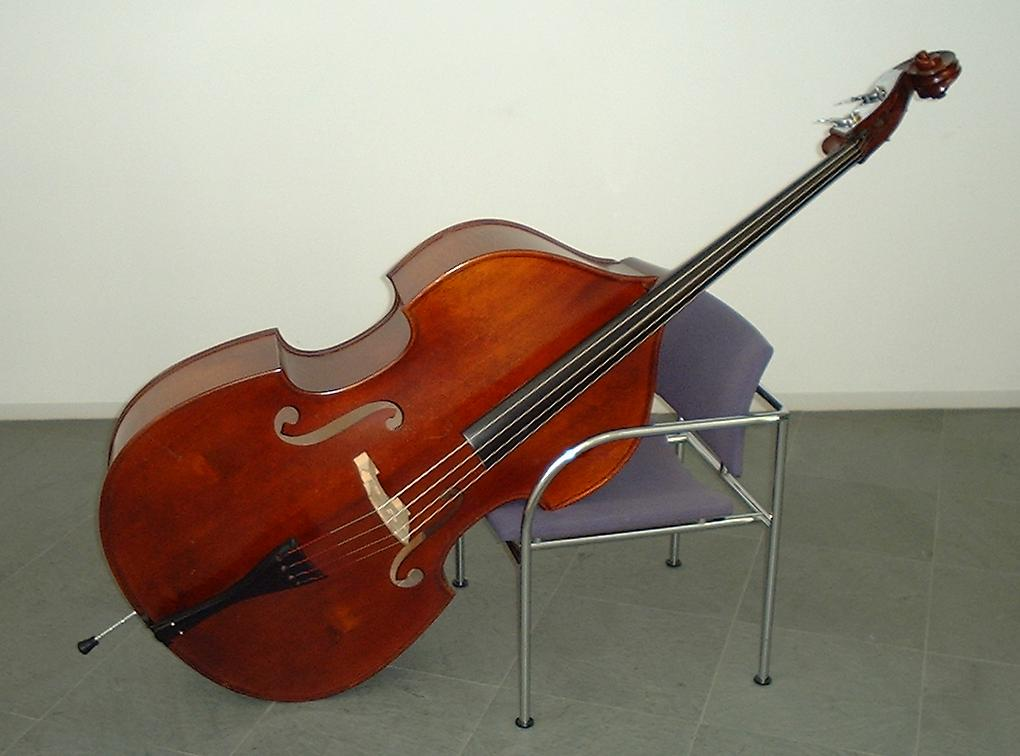
\includegraphics[height=2.7cm]{Pics/Instrument/on_chair.epsi}\\
{\small 図\thefigure : 椅子に立てかける場合\\}
\end{center}
\end{minipage}
\hfill
\begin{minipage}{200pt}
\addtocounter{figure}{1}
\begin{center}
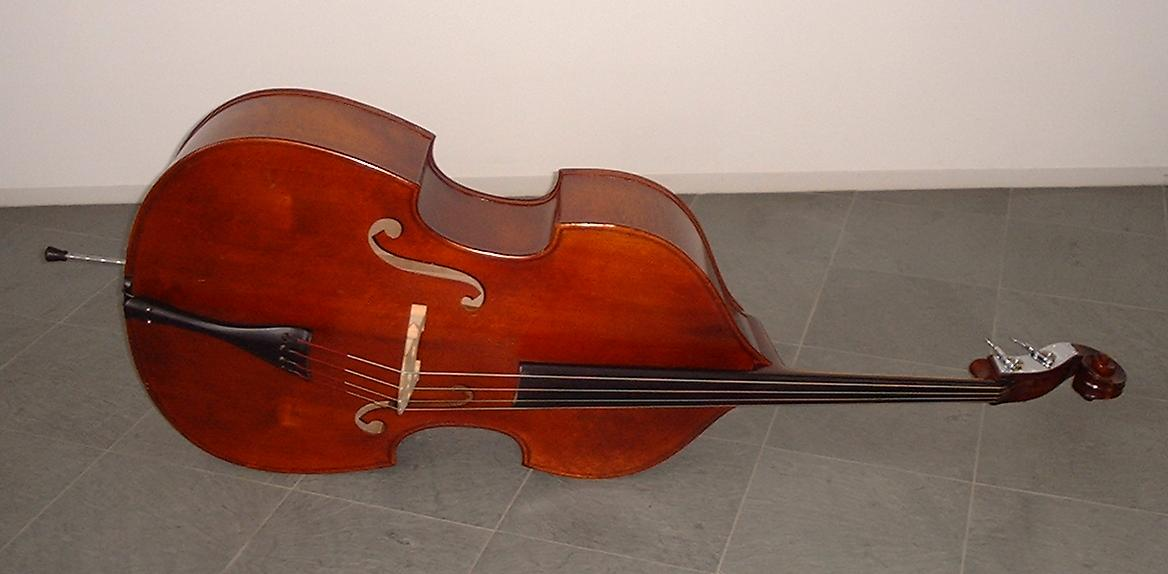
\includegraphics[height=2.7cm]{Pics/Instrument/on_earth.epsi}\\
{\small 図\thefigure : 床に置く場合\\}
\end{center}
\end{minipage}


\subsection{楽器の支え方}

図\addtocounter{figure}{1}\thefigure と図
\addtocounter{figure}{1}\thefigure の点線部分を対応させるようにして楽
器を体に当てます。\\
%ネックを持つ左手を除いて
%は、点線部分以外の部位で楽器に触れることはありません。\\

\addtocounter{figure}{-1}
\begin{minipage}{150pt}
\begin{center}

\includegraphics[height=7.35cm]{Pics/Instrument/standing.epsi}\\
{\small 図\thefigure : 足の付け根(点線部分)で支える\\}
\end{center}
\end{minipage}
\hfill
\begin{minipage}{110pt}
\begin{center}
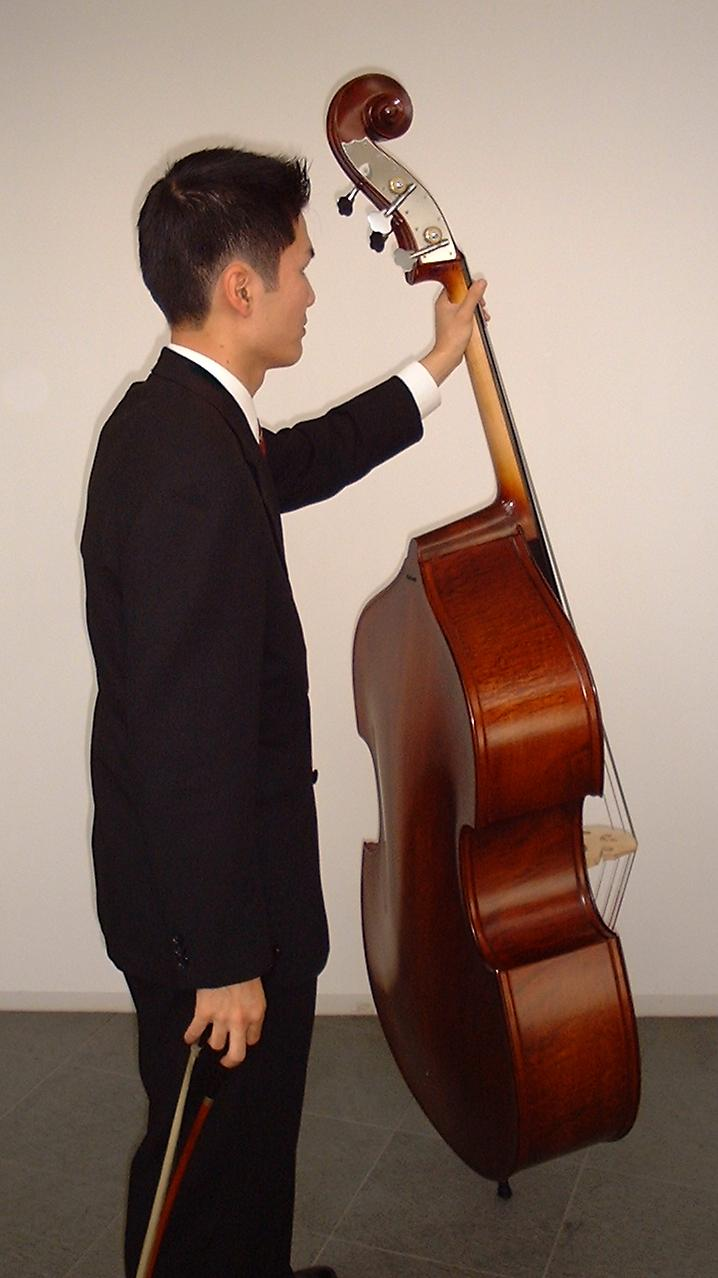
\includegraphics[height=7.35cm]{Pics/Instrument/edge.epsi}\\
\addtocounter{figure}{1}
{\small 図\thefigure : 点線は体に当てる部分\\}
\end{center}
\end{minipage}
\hfill
\begin{minipage}{140pt}
\begin{center}
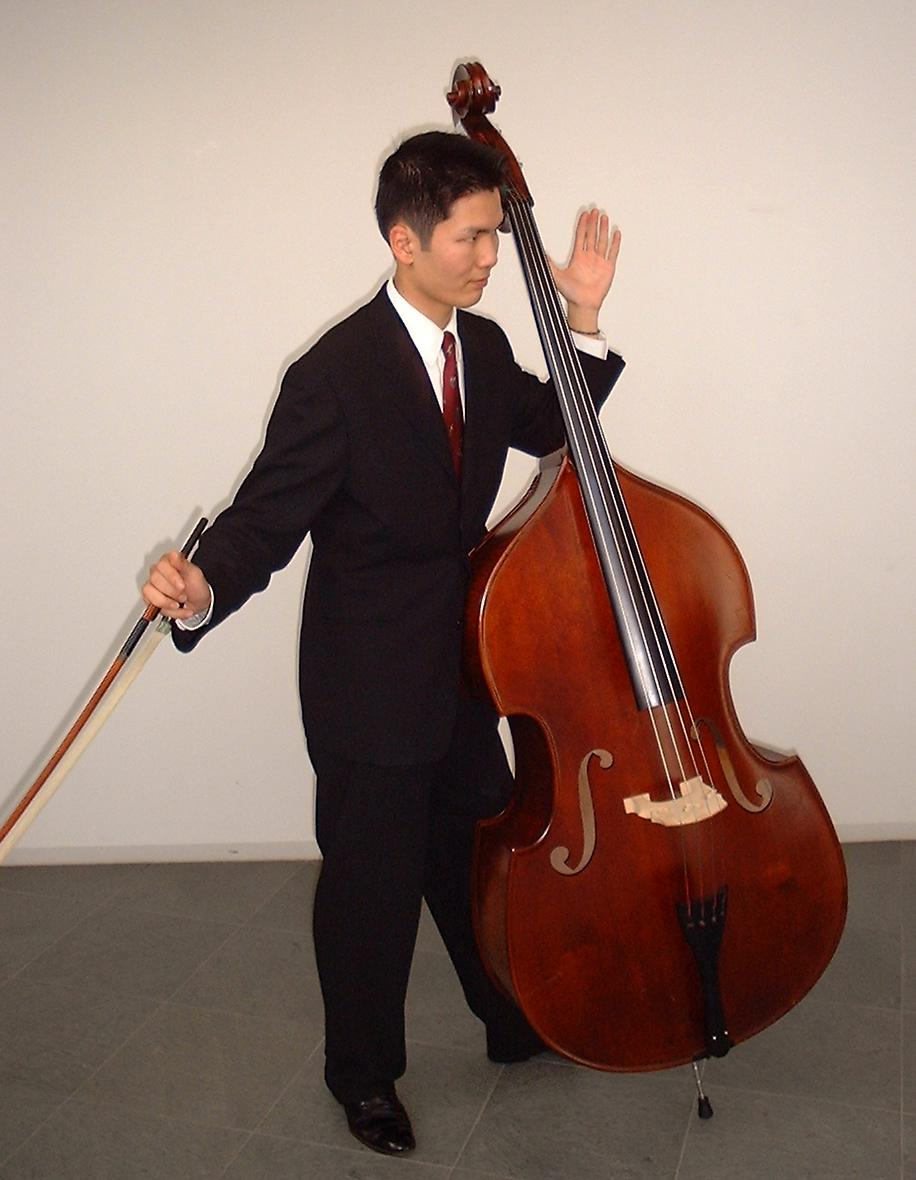
\includegraphics[height=7.35cm]{Pics/Instrument/without_hands.epsi}\\
\addtocounter{figure}{1}
{\small 図\thefigure : 手を触れずに支えるのが理想}
\end{center}
\end{minipage}

\ \\
\ \\


\begin{minipage}{190pt}
\ \ \ \ \addtocounter{figure}{-2}図\thefigure と図
\addtocounter{figure}{1}\thefigure の点線部分どうしをうまく対応させられない場合には、エンドピンの長さを調節して楽器の高さを合わせます。エンドピンとは楽器胴体の下端にネジで固定されている金属棒のことです。
\end{minipage}
\hfill
\begin{minipage}{220pt}
\begin{center}
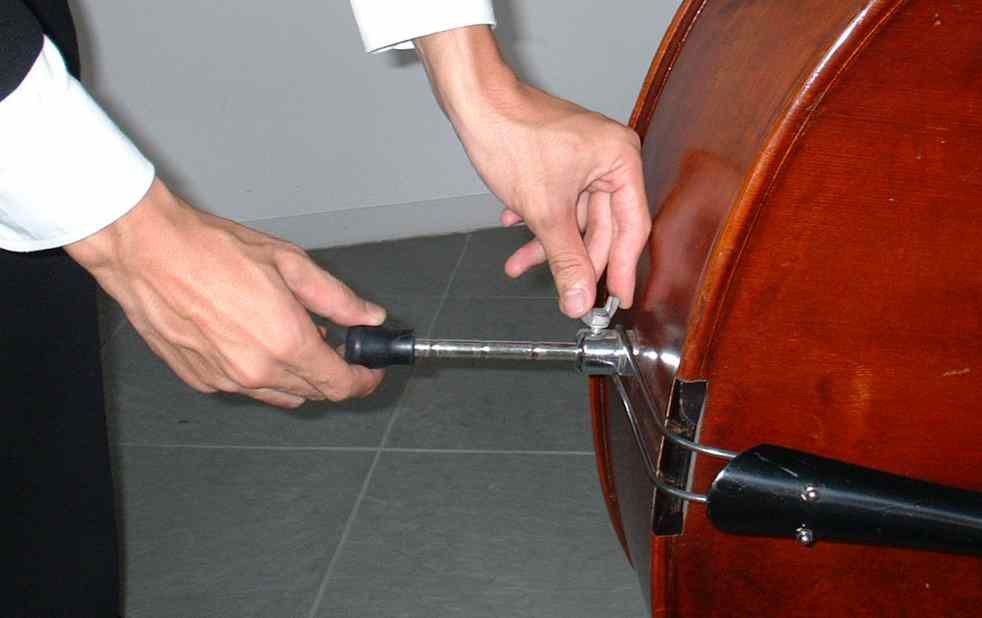
\includegraphics[height=3cm]{Pics/photo0830/endpin.epsi}\\
\addtocounter{figure}{2}
{\small 図\thefigure : ネジを緩めてエンドピンの長さを調節}
\end{center}
\end{minipage}

\ \\
\ \\

\begin{minipage}{120pt}
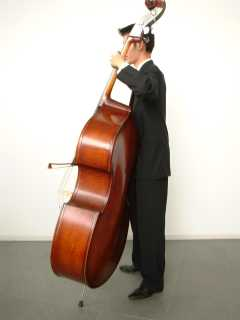
\includegraphics[height=7cm]{Pics/photo0830/stand_left.epsi}\\
\addtocounter{figure}{1}
{\small 図\thefigure : 楽器の支え方(左側から)}
\end{minipage}
\hfill
\begin{minipage}{120pt}
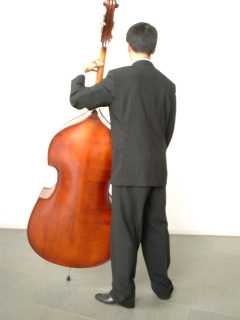
\includegraphics[height=7cm]{Pics/photo0830/stand_back.epsi}\\
\addtocounter{figure}{1}
{\small 図\thefigure : 楽器の支え方(背面から)}
\end{minipage}
\hfill
\begin{minipage}{120pt}
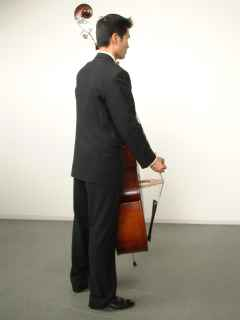
\includegraphics[height=7cm]{Pics/photo0830/stand_right.epsi}\\
\addtocounter{figure}{1}
{\small 図\thefigure : 楽器の支え方(右側から)}
\end{minipage}


\subsection{弓の毛}
弓の毛の張りは末端のネジで調節します。弾くときに張り、弾かないときは緩
めておきます。適度な弓の張りの目安は以下の2点を同時に満たすことです。

\begin{enumerate}
\item 弦に乗せて圧力をかけても竿が毛に触れない
\item 竿が反っている
\end{enumerate}

図\addtocounter{figure}{2}\thefigure のように竿に反りがない弓は明らか
に張りすぎです。弓の毛は消耗品ですので、1 年をめどに楽器店で交換しましょ
う。また、直接手で触れてはいけません。皮脂が付着して松ヤニの乗りが悪く
なります。\addtocounter{figure}{-1}
\begin{center}
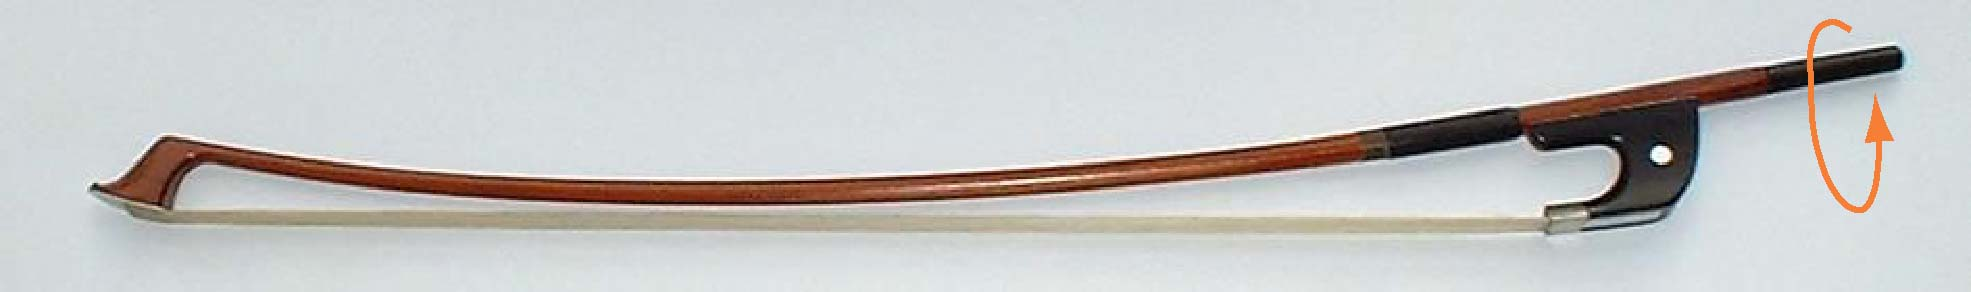
\includegraphics[width=13.5cm]{Pics/Bow/whole_bow_arrow.epsi}\\
{\small 図\thefigure : ネジを矢印の方向に回すと毛が緩む\\}
\end{center}
\addtocounter{figure}{1}
\begin{center}
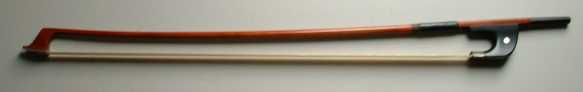
\includegraphics[width=13.5cm]{Pics/photo0830/tense_bow.epsi}\\
{\small 図\thefigure : 竿に反りがないのは張りすぎ\\}
\end{center}

\subsection{松ヤニ}
弓のすべり止めです。弓の毛と弦の間に松ヤニ粒子が介在して摩擦力が発生し
ます。弓毛を張ったら\addtocounter{figure}{2}図\thefigure のようにして
弓毛に塗付してください。また、練習終了後には弦に付着した松ヤニをタオル
で拭き取るようにしましょう\addtocounter{figure}{1}(図\thefigure )。\\
\indent 弦に付着した松ヤニと弓の松ヤニが異なると好ましくありません。な
るべくパート全員が同じ銘柄のものを使うようにしましょう。高温にさらすと
液化・変性してしまうので使用後はケースに入れて涼しい場所に保管します。

\begin{minipage}{180pt}
\addtocounter{figure}{-2}
\begin{center}
\includegraphics[height=3.5cm]{Pics/photo0830/rosin.epsi}\\
{\small 図\thefigure : 松ヤニとケース\\}
\end{center}
\end{minipage}
\hfill
\begin{minipage}{120pt}
\addtocounter{figure}{1}
\begin{center}
\includegraphics[height=3.5cm]{Pics/newphoto/rosin.epsi}\\
{\small 図\thefigure : 弓毛を張ったら塗る\\}
\end{center}
\end{minipage}
\hfill
\begin{minipage}{100pt}
\addtocounter{figure}{1}
\begin{center}
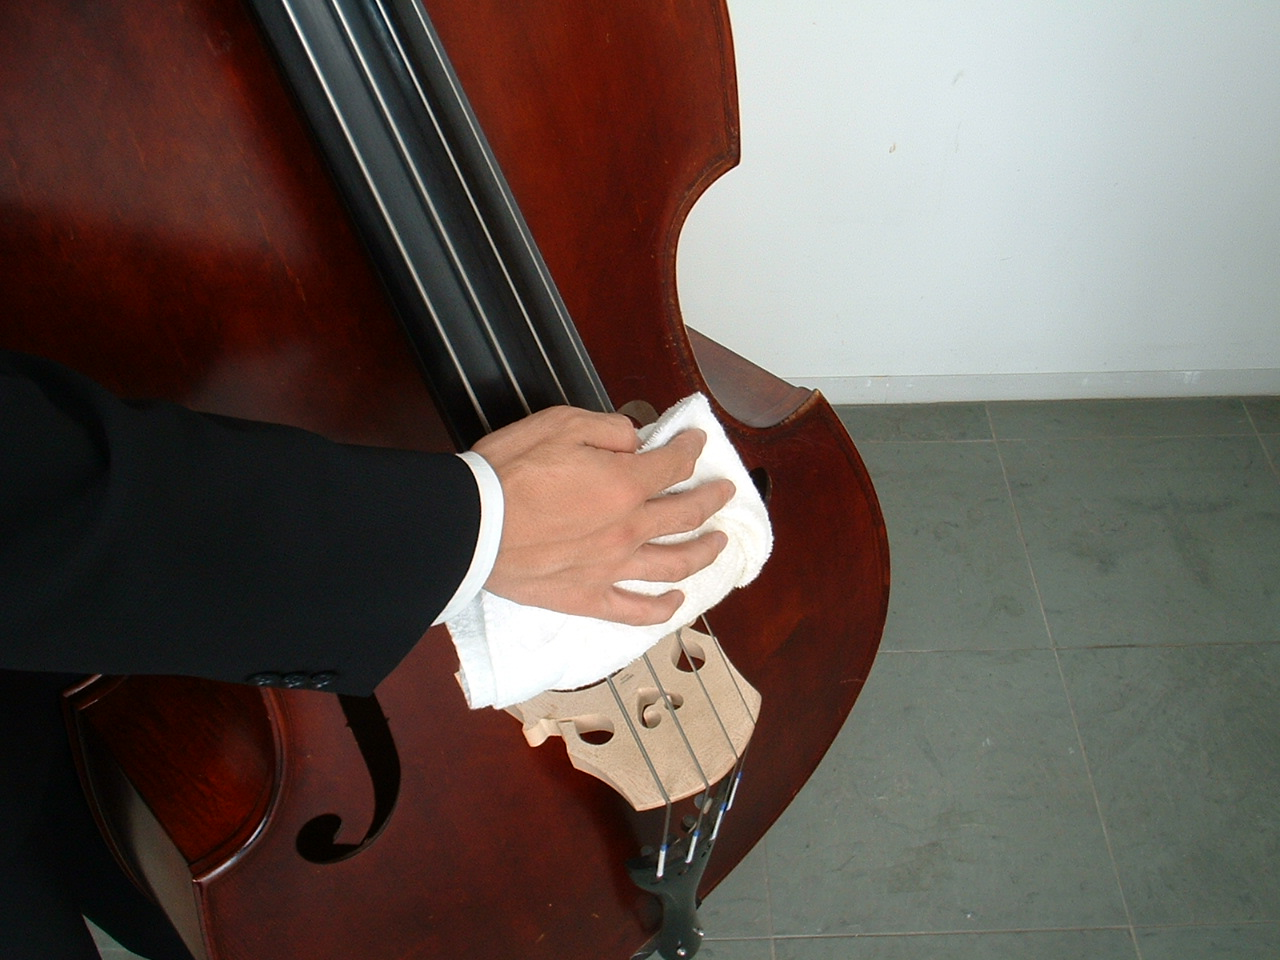
\includegraphics[height=3.5cm]{Pics/newphoto/towel.epsi}\\
{\small 図\thefigure : 練習後は拭き取る\\}
\end{center}
\end{minipage}

\subsection{弓の持ち方: (1) ドイツ式}
\underline{\bf 弓は主に親指と小指で持ちます}。図\addtocounter{figure}{1}\thefigure 〜図\addtocounter{figure}{3}\thefigure の順序に従って弓を持ってみましょう。\\

\begin{minipage}{200pt}
\begin{center}
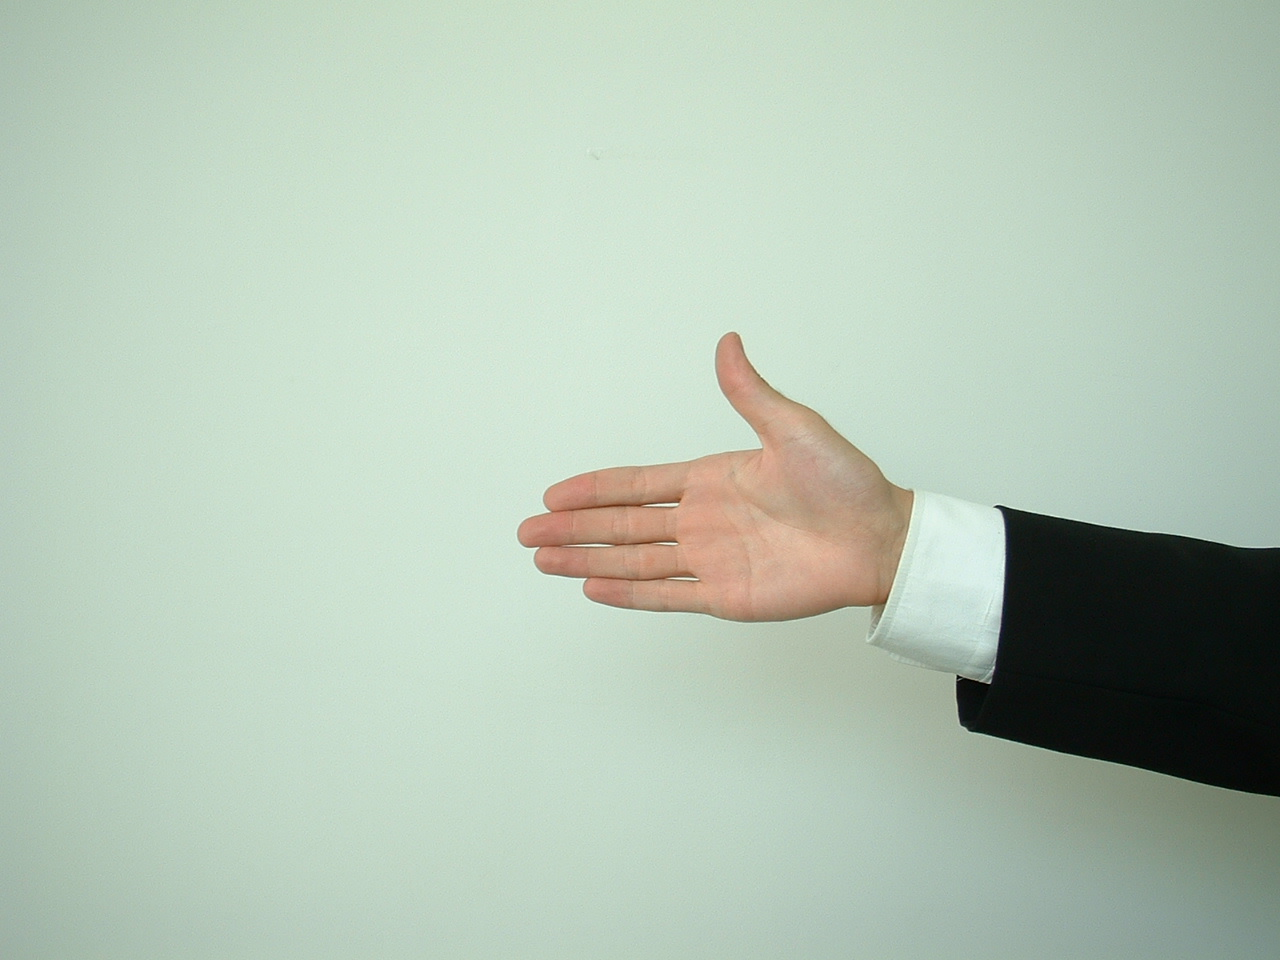
\includegraphics[height=4.3cm]{Pics/photo0830/righthand2.epsi}\\
\addtocounter{figure}{-3}
{\small 図\thefigure : 右手を構える\\}
\end{center}
\end{minipage}
\hfill
\begin{minipage}{200pt}
\begin{center}
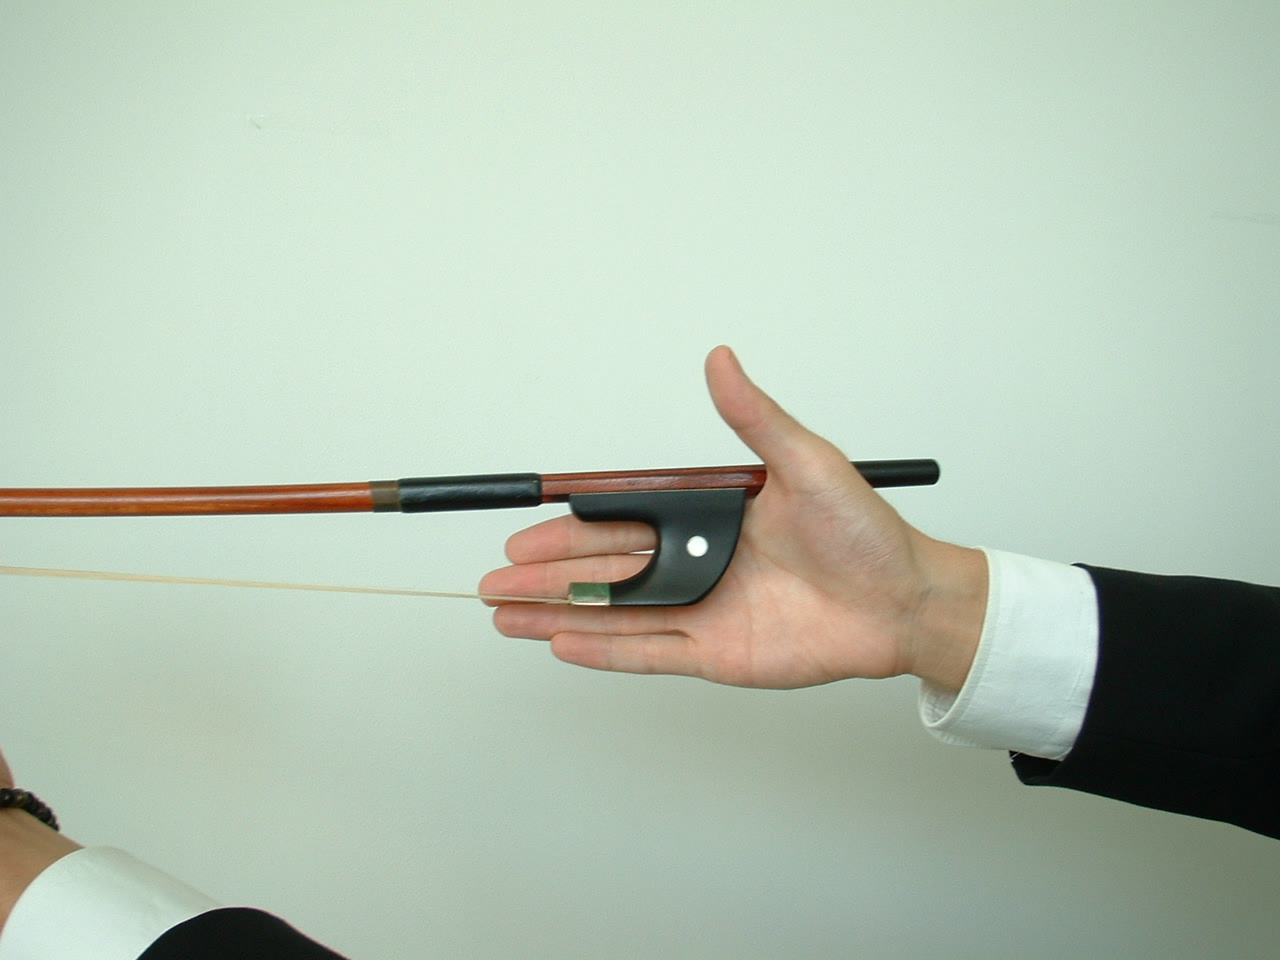
\includegraphics[height=4.3cm]{Pics/photo0830/righthand4.epsi}\\
\addtocounter{figure}{1}
{\small 図\thefigure : 弓の尾部を親指と人さし指の間に入れる\\}
\end{center}
\end{minipage}

\begin{minipage}{220pt}
\begin{center}
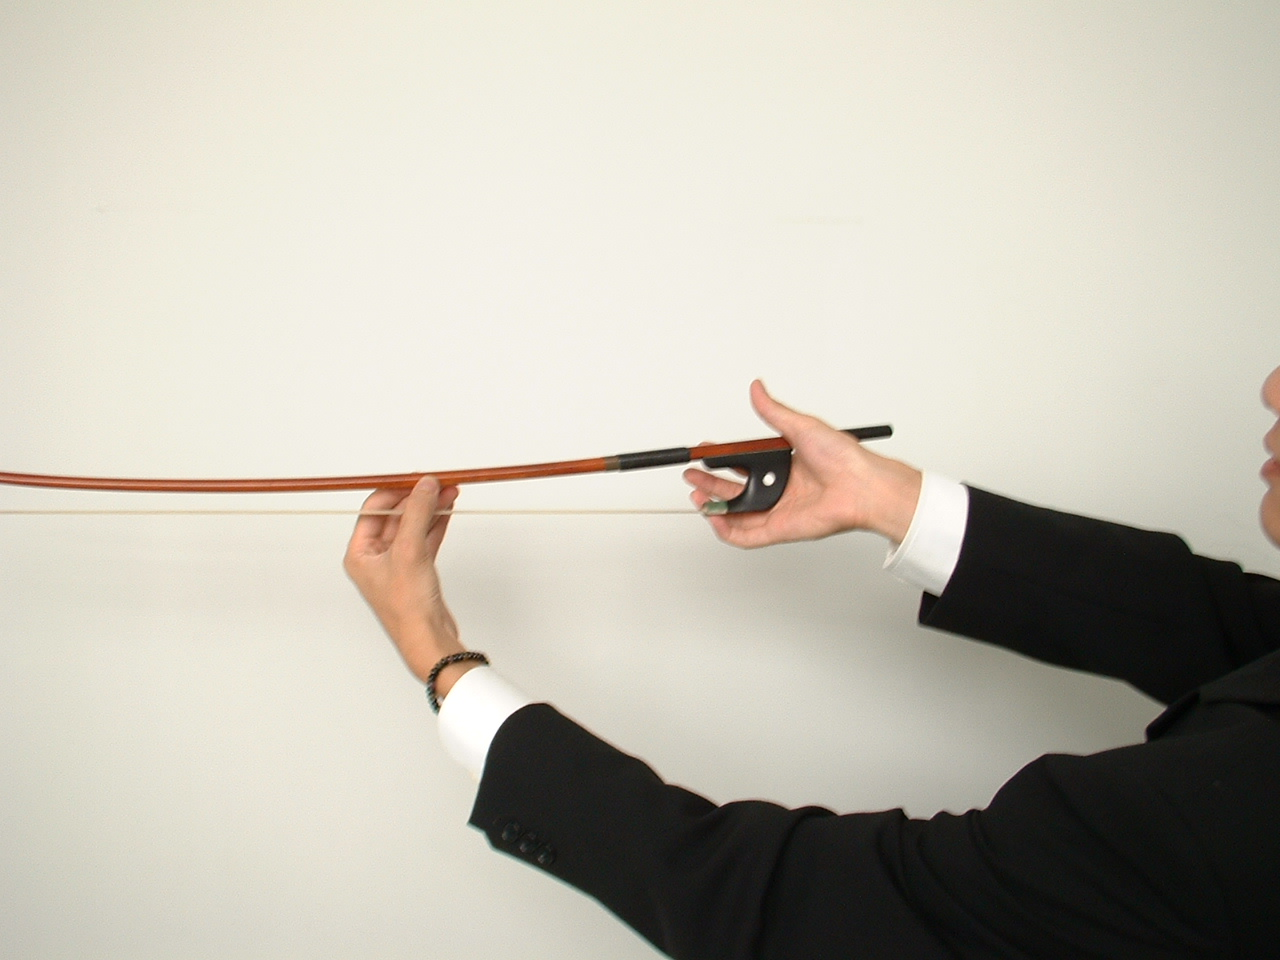
\includegraphics[height=4.3cm]{Pics/photo0830/bow3.epsi}\\
\addtocounter{figure}{1}
{\small 図\thefigure : 小指を丸めて金具を押さえる(図\addtocounter{figure}{2}\thefigure、図\addtocounter{figure}{1}\thefigure 参照)\\}
\end{center}
\end{minipage}
\hfill
\begin{minipage}{200pt}
\begin{center}
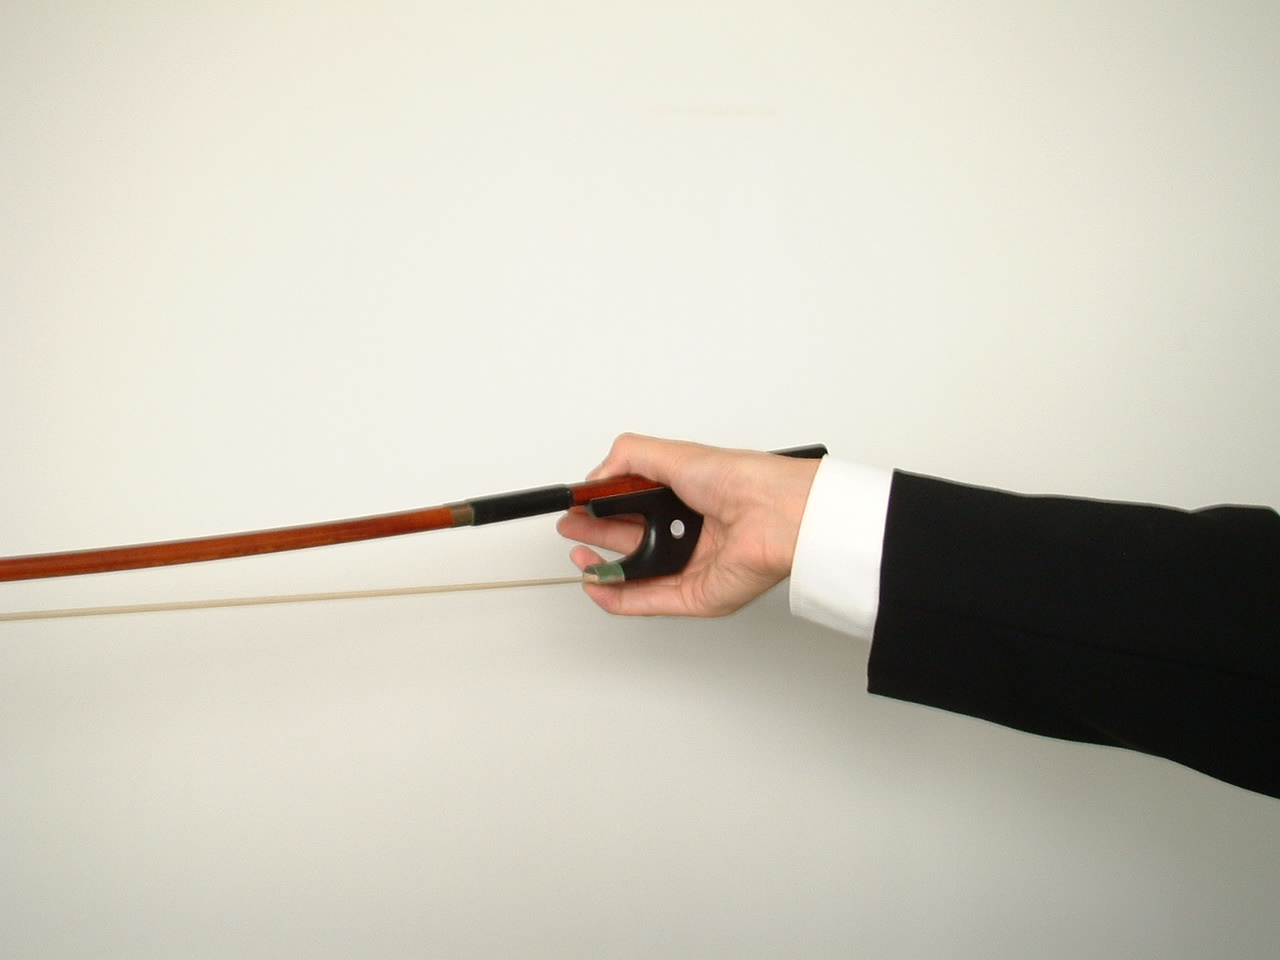
\includegraphics[height=4.3cm]{Pics/photo0830/bow4.epsi}\\
\addtocounter{figure}{-2}
{\small 図\thefigure : 親指を竿にかける(図\addtocounter{figure}{3}\thefigure〜\addtocounter{figure}{2}\thefigure 参照)\\}
\end{center}
\end{minipage}

\ \\

図\addtocounter{figure}{-6}\thefigure では小指を丸め、指先で弓毛の端にある金具を押さえます(図\addtocounter{figure}{2}\thefigure に網目で示した部分)。正しく押さえると図\addtocounter{figure}{1}\thefigure のようになります。また、図\addtocounter{figure}{-2}\thefigure において親指で竿を押さえる際には図\addtocounter{figure}{3}\thefigure 、\addtocounter{figure}{1}\thefigure に網目で示した部分どうしを重ね合わせ、図\addtocounter{figure}{1}\thefigure のようにします。\\

\begin{minipage}{120pt}
\addtocounter{figure}{-4}
\begin{center}
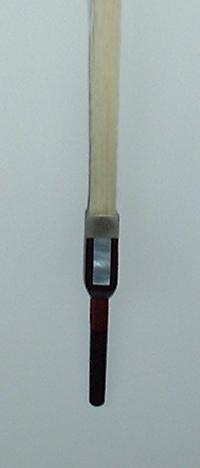
\includegraphics[height=8.8cm]{Pics/Bow/smallfinger_area.epsi}\\
{\small 図\thefigure : 小指が押さえる金具\\}
\end{center}
\end{minipage}
\hfill
\begin{minipage}{100pt}
\begin{center}
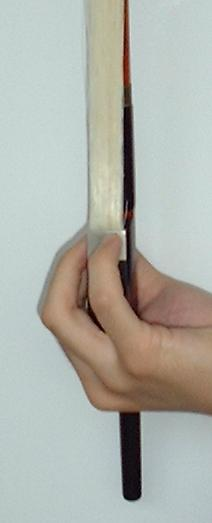
\includegraphics[height=8.8cm]{Pics/Bow/smallfinger.epsi}\\
\addtocounter{figure}{1}
{\small 図\thefigure : 小指\\}
\end{center}
\end{minipage}
\hfill
\begin{minipage}{110pt}
\addtocounter{figure}{1}
\begin{center}

\includegraphics[width=2cm]{Pics/Bow/thumb.epsi}\\
{\small 図\thefigure : 親指と竿の接触部分(網目部分)\\}
\addtocounter{figure}{1}
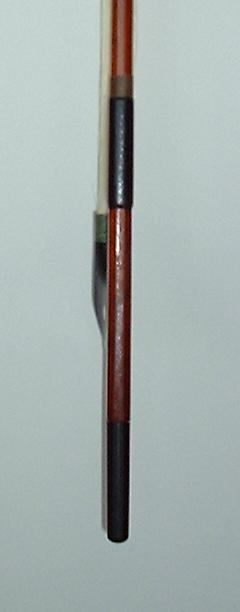
\includegraphics[width=2cm]{Pics/Bow/thumb_area.epsi}\\
{\small 図\thefigure : 親指と竿の接触部分(網目部分)\\}
\end{center}
\end{minipage}
\hfill
\begin{minipage}{80pt}
\addtocounter{figure}{1}
\begin{center}
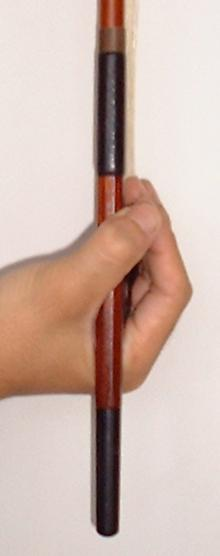
\includegraphics[height=8.8cm]{Pics/Bow/thumb_and_bow.epsi}\\
{\small 図\thefigure : 親指と竿\\}
\end{center}
\end{minipage}

以上の手続きに従って正しく弓を持てたときの手の形を図
\addtocounter{figure}{1}\thefigure 〜図
\addtocounter{figure}{2}\thefigure に示しました。なお、初心者にありが
ちな間違いとして図\addtocounter{figure}{1}\thefigure のように竿と弓毛
の間に人さし指、中指、薬指のいずれかを入れることが見られますが、これは
手首の柔軟な動きを損なうので避けましょう。\\\underline{\bf 親指・小指以
外の中3本の指は軽く添えるだけです}。\\

\begin{minipage}{210pt}
\addtocounter{figure}{-3}
\begin{center}
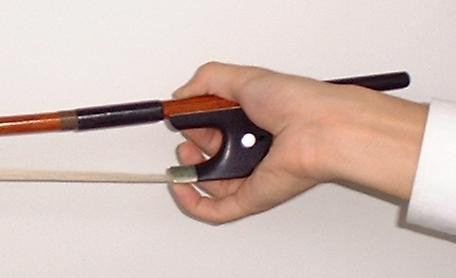
\includegraphics[height=4.3cm]{Pics/Bow/perspective_1.epsi}\\
{\small 図\thefigure : 弓の持ち方(手の平側)}
\end{center}
\end{minipage}
\hfill
\begin{minipage}{210pt}
\addtocounter{figure}{1}
\begin{center}
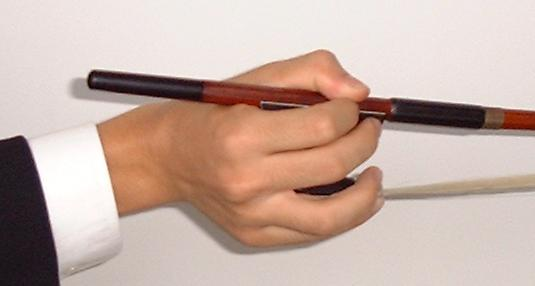
\includegraphics[height=4.3cm]{Pics/Bow/perspective_2.epsi}\\
{\small 図\thefigure : 弓の持ち方(手の甲側)}
\end{center}
\end{minipage}

\begin{minipage}{200pt}
\begin{center}
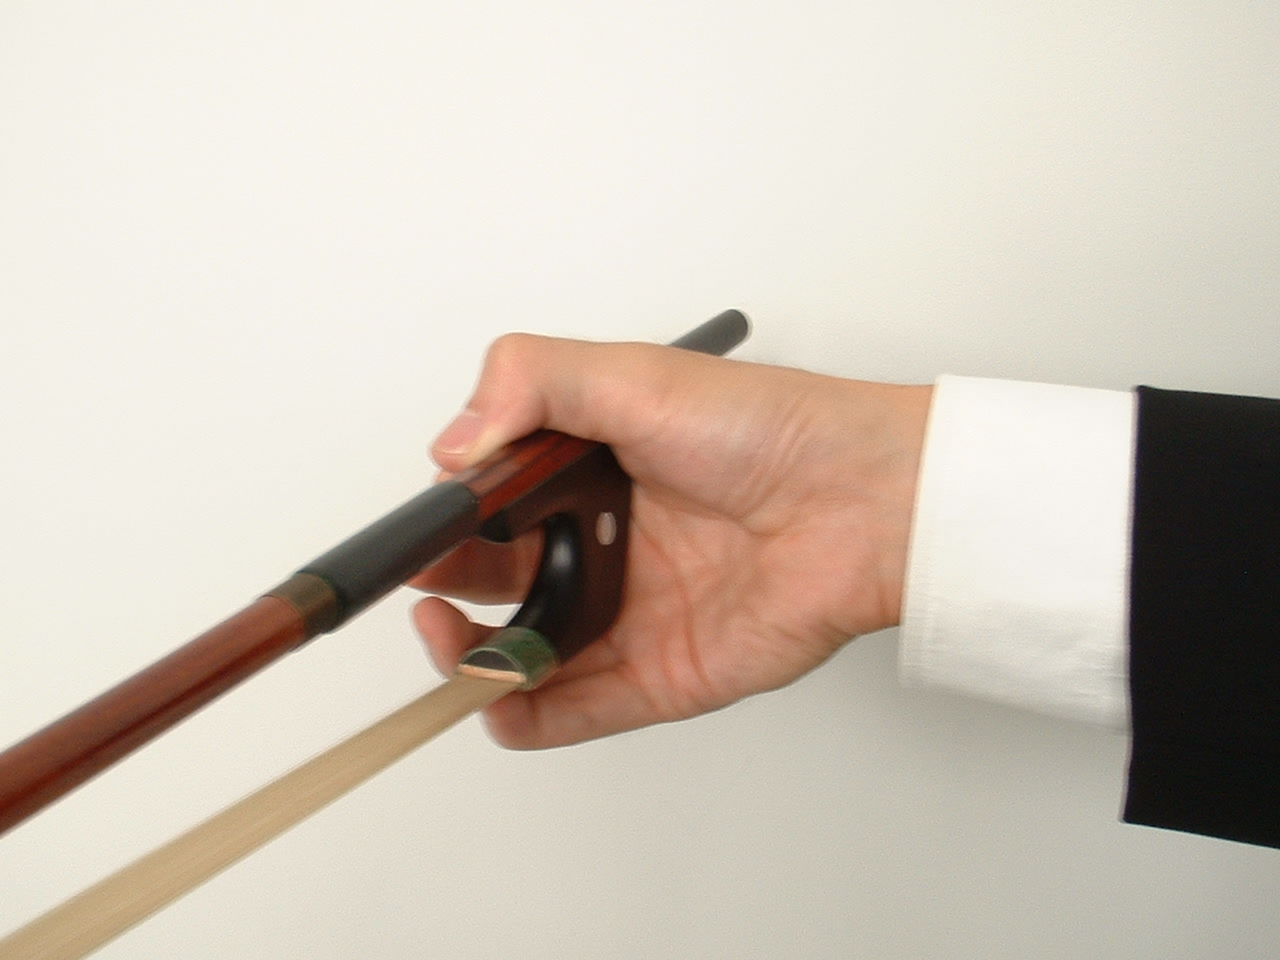
\includegraphics[height=4.3cm]{Pics/photo0830/bow5.epsi}\\
\addtocounter{figure}{1}
{\small 図\thefigure : 手の平は毛箱を包み込むように\\}
\end{center}
\end{minipage}
\hfill
\begin{minipage}{200pt}
\begin{center}
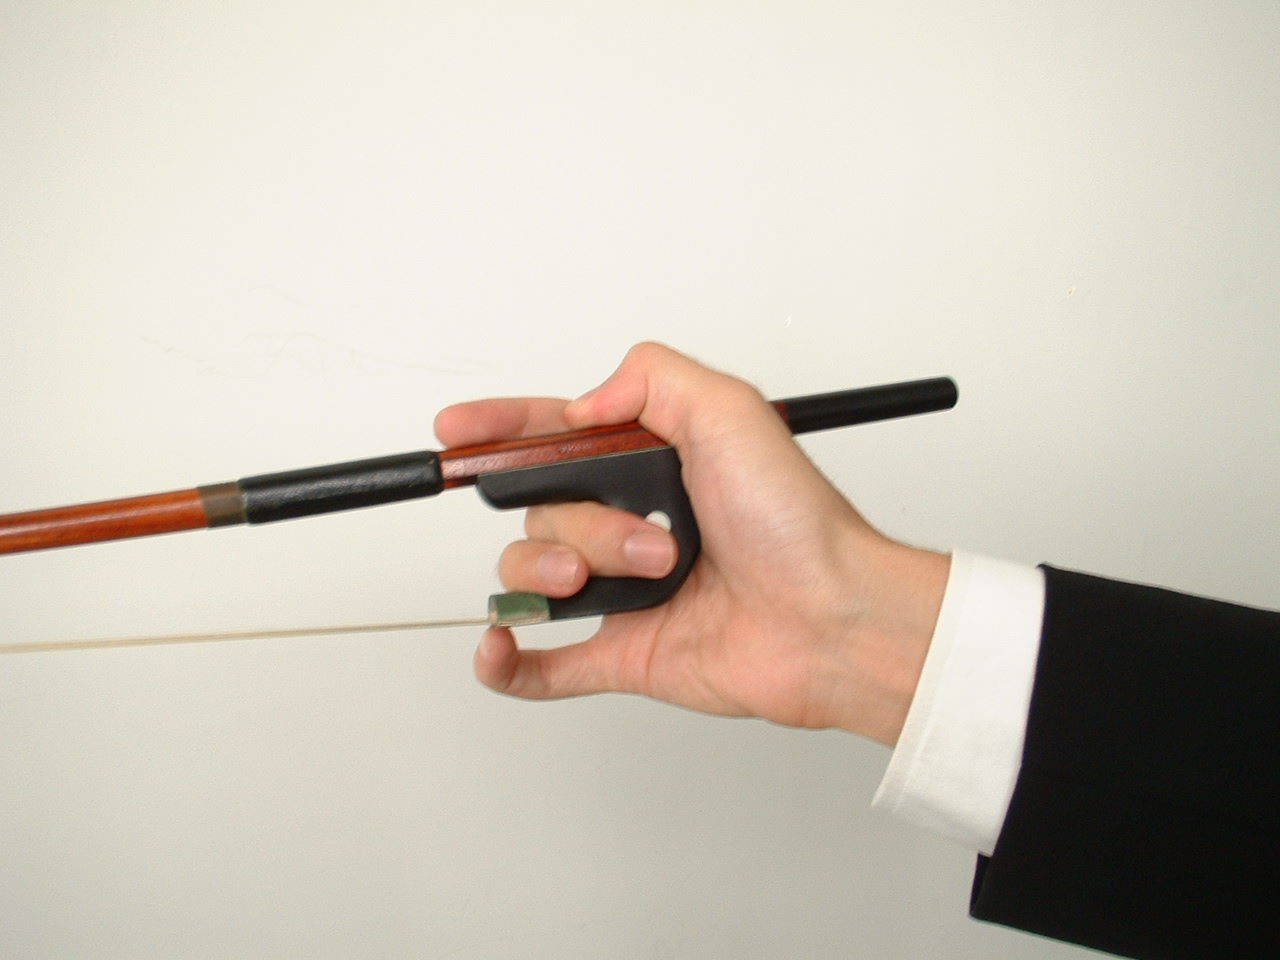
\includegraphics[height=4.3cm]{Pics/photo0830/badbow.epsi}\\
\addtocounter{figure}{1}
{\small 図\thefigure : 悪い例(竿と弓毛の間に指を入れない)\\}
\end{center}
\end{minipage}

\subsection{弓の持ち方: (2) フランス式}



\subsection{弓で弦を弾く}
弓は\ruby{指}{し}\ruby{板}{ばん}の端から駒までの間に置きます(図
\addtocounter{figure}{1}\thefigure)。弓の軌道が弦に対して垂直に交差す
るように動かします(図\addtocounter{figure}{1}\thefigure)。鏡を利用して
弓の軌道を確認しながら練習するのも有効でしょう。どの弦でもいいので、以
下の順序に従って音を鳴らしてみましょう。

\begin{flushleft}
\begin{minipage}{200pt}

\begin{enumerate}
\item 竿を指板側に少し傾ける(図\addtocounter{figure}{1}\thefigure 、\addtocounter{figure}{1}\thefigure) 
\item 親指に力を入れて弦に圧力をかける
\item 弓を動かす
\item 音が鳴りだしたら親指の力を抜く。弓は動かし続ける。
\end{enumerate}
\end{minipage}
\hfill
\begin{minipage}{110pt}
\begin{center}
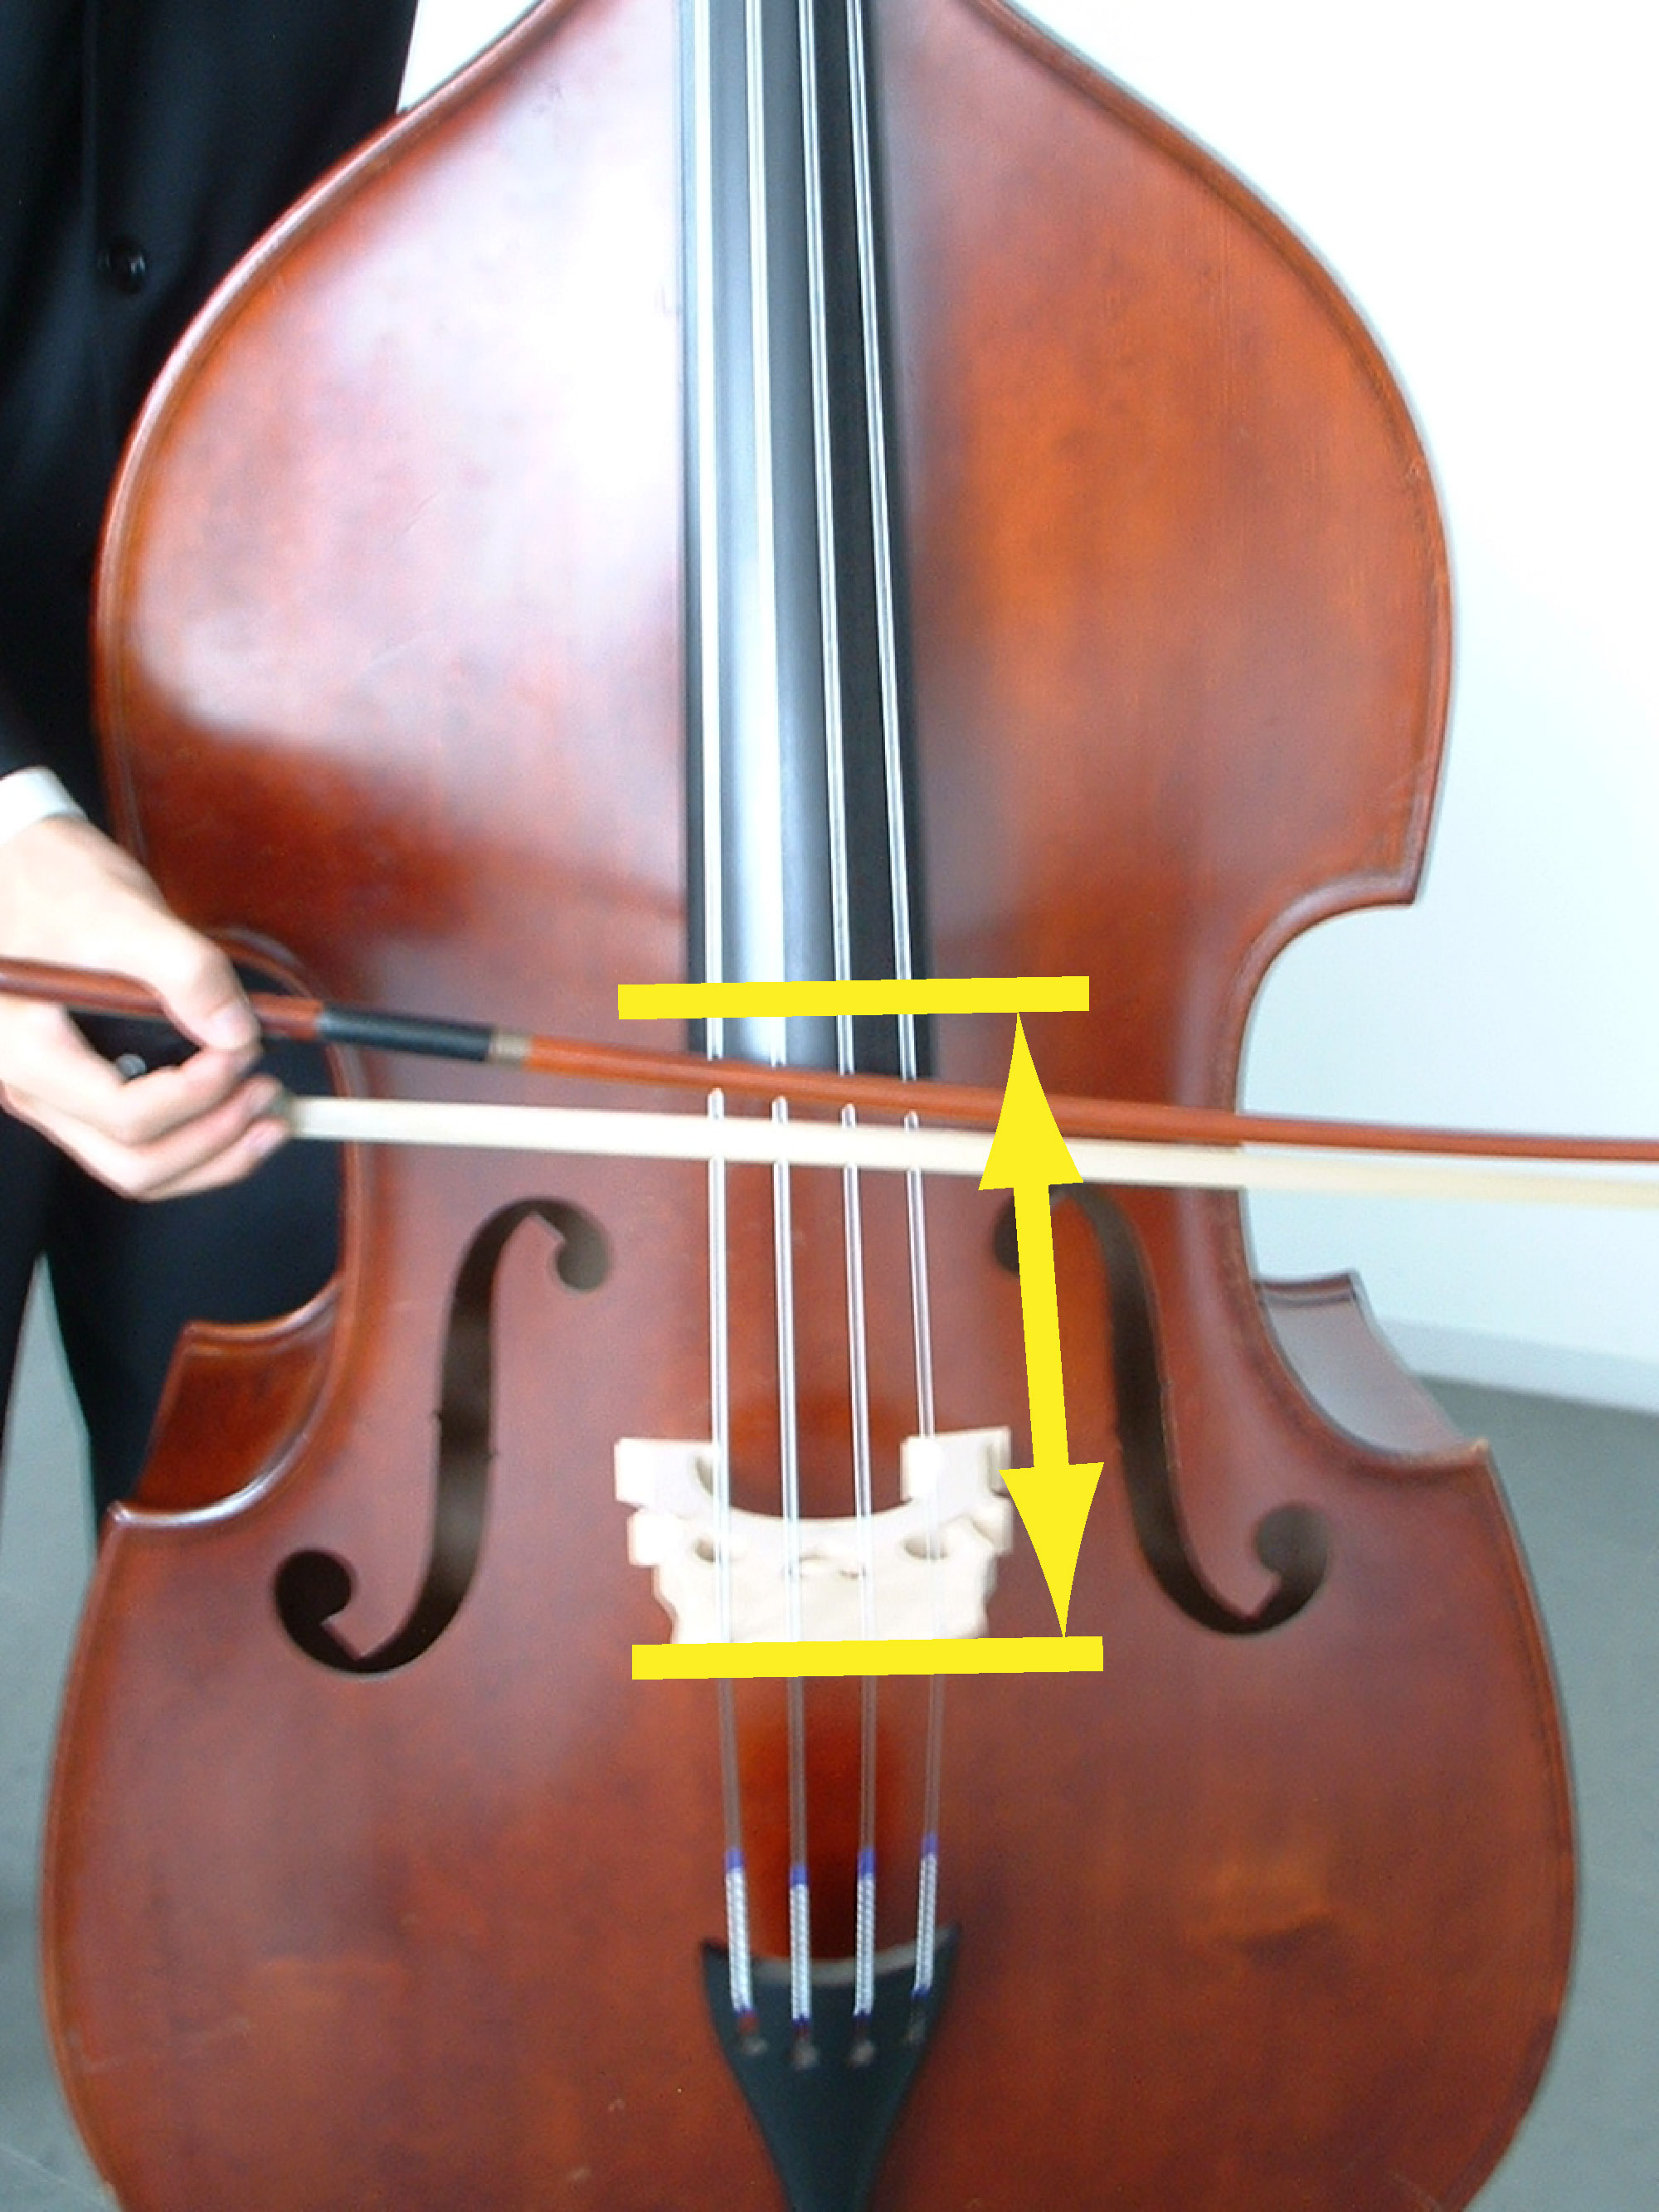
\includegraphics[height=3.4cm]{Pics/photo0830/bowbass2.epsi}\\
\addtocounter{figure}{-3}
{\small 図\thefigure : 矢印の範囲内を弾く\\}
\end{center}
\end{minipage}
\hfill
\begin{minipage}{110pt}
\begin{center}
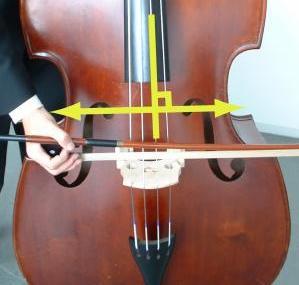
\includegraphics[height=3.4cm]{Pics/photo0830/bowbass1.epsi}\\
\addtocounter{figure}{1}
{\small 図\thefigure : 弓の軌道は弦と直交\\}
\end{center}
\end{minipage}

\begin{minipage}{205pt}
\ \ \ \ 親指の力がうまく弦に伝わると、振幅がはっきりと見えるほど弦が振
動します。一旦振動が始まったら、親指から力を抜きます。あとは弓を動かし
ているだけで振動を保つことができます。\\
\end{minipage}
\hfill
\begin{minipage}{110pt}
\begin{center}
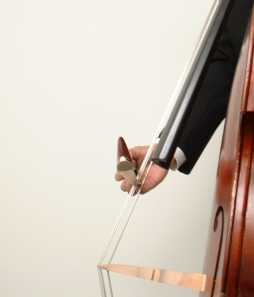
\includegraphics[height=4cm]{Pics/photo0830/bow_string1.epsi}\\
\addtocounter{figure}{1}
{\small 図\thefigure : 竿を指板側に傾ける\\}
\end{center}
\end{minipage}
\hfill
\begin{minipage}{110pt}
\begin{center}
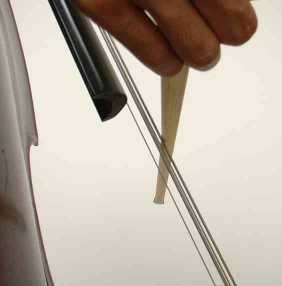
\includegraphics[height=4cm]{Pics/photo0830/bow_string2.epsi}\\
\addtocounter{figure}{1}
{\small 図\thefigure : 右側から見た図\\}
\end{center}
\end{minipage}
\end{flushleft}

\clearpage

\subsection{音量}
大まかに言って、音量は以下の4要素の組合せで決まります。\\

\begin{quote}
\begin{enumerate}
\item 右手親指の圧力\  (強いほど音量大)
\item 駒からの距離\ \ \ \  (駒に近いほど音量大)
\item 弓先か弓元か\ \ \ \ (弓の先ほど繊細な音を出しやすい)
\item 弓を動かす速さ\  (速ければ力強い音、ゆっくりなら柔和な音)
\end{enumerate}
\end{quote}

音量や音色は奥が深いテーマですので、本書ではこれ以上立ち入らないことにします。

\subsection{開放弦}
左手で弦を押さえていない状態のことを\underline{\bf 開放弦}と呼びます。コントラバスの開放弦は太い方から順にE\(\longrightarrow\)A\(\longrightarrow\)D\(\longrightarrow\)Gというよ
うに4度ずつ上がっていきます\footnote{ヴィオラ、チェロはヴァイオリンを原型とする「ヴァイオリン属」に含まれ、太い弦から順に5度ずつ上がる。一方、コントラバスは前3者とは異なりヴィオールという楽器を原型とする「ヴィオール属」である。調弦の違いはここに由来する。}。

\begin{music}
\nostartrule
\parindent 0pt
\setclef1{\bass}  
\startextract
\Notes\zchar{-7}{\ \ \ \ \ E}\enotes
\NOTEs\wh{E}\enotes
\doublebar
\Notes\zchar{-7}{\ \ \ \ \ A}\enotes
\NOTEs\wh{'A}\enotes
\doublebar
\Notes\zchar{-7}{\ \ \ \ \ D}\enotes
\NOTEs\wh{'D}\enotes
\doublebar
\Notes\zchar{-7}{\ \ \ \ \ G}\enotes
\NOTEs\wh{'G}\enotes
\setdoublebar
\endextract
\end{music}


なお、記譜上の慣習として、コントラバスの譜面は実音よりも1オクターヴ上に書かれます。逆に言えば、楽譜に書かれた音を弾くと、コントラバスはその1オクターヴ下の音を出します。

\subsection{チューニングメーター}
\begin{flushleft}
\begin{minipage}{320pt}
\ \ \ \ \ 音程を合わせる装置です。練習を始める前には必ずチューニングメー
ターを用いて開放弦の音程を合わせておきましょう。
\addtocounter{figure}{3}図\thefigure のようにしてコンタクトマイクを通
して集音すれば、うるさい場所でも確実に自分の楽器の音を拾ってくれます。
\\

\begin{minipage}{150pt}
\addtocounter{figure}{-2}
\begin{center}
\includegraphics[width=3cm]{Pics/newphoto/tuner.epsi}\\
{\small 図\thefigure : チューニングメーター\\}
\end{center}
\end{minipage}
\hfill
\begin{minipage}{150pt}
\addtocounter{figure}{1}
\begin{center}
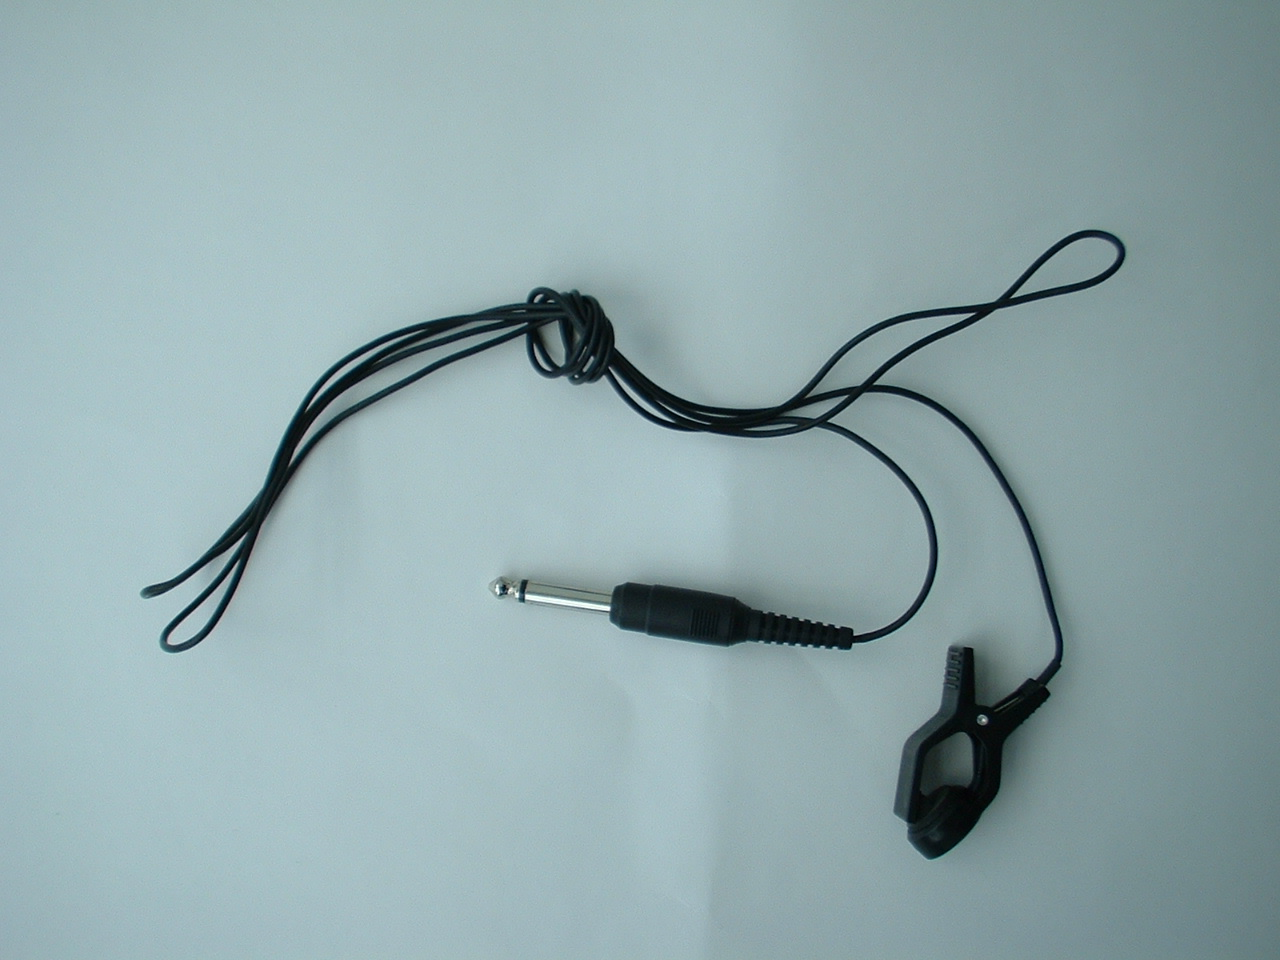
\includegraphics[width=2.7cm]{Pics/newphoto/contact1.epsi}\\
{\small 図\thefigure : コンタクトマイク\\}
\end{center}
\end{minipage}
\end{minipage}
\hfill
\begin{minipage}{110pt}
\addtocounter{figure}{1}
\begin{center}
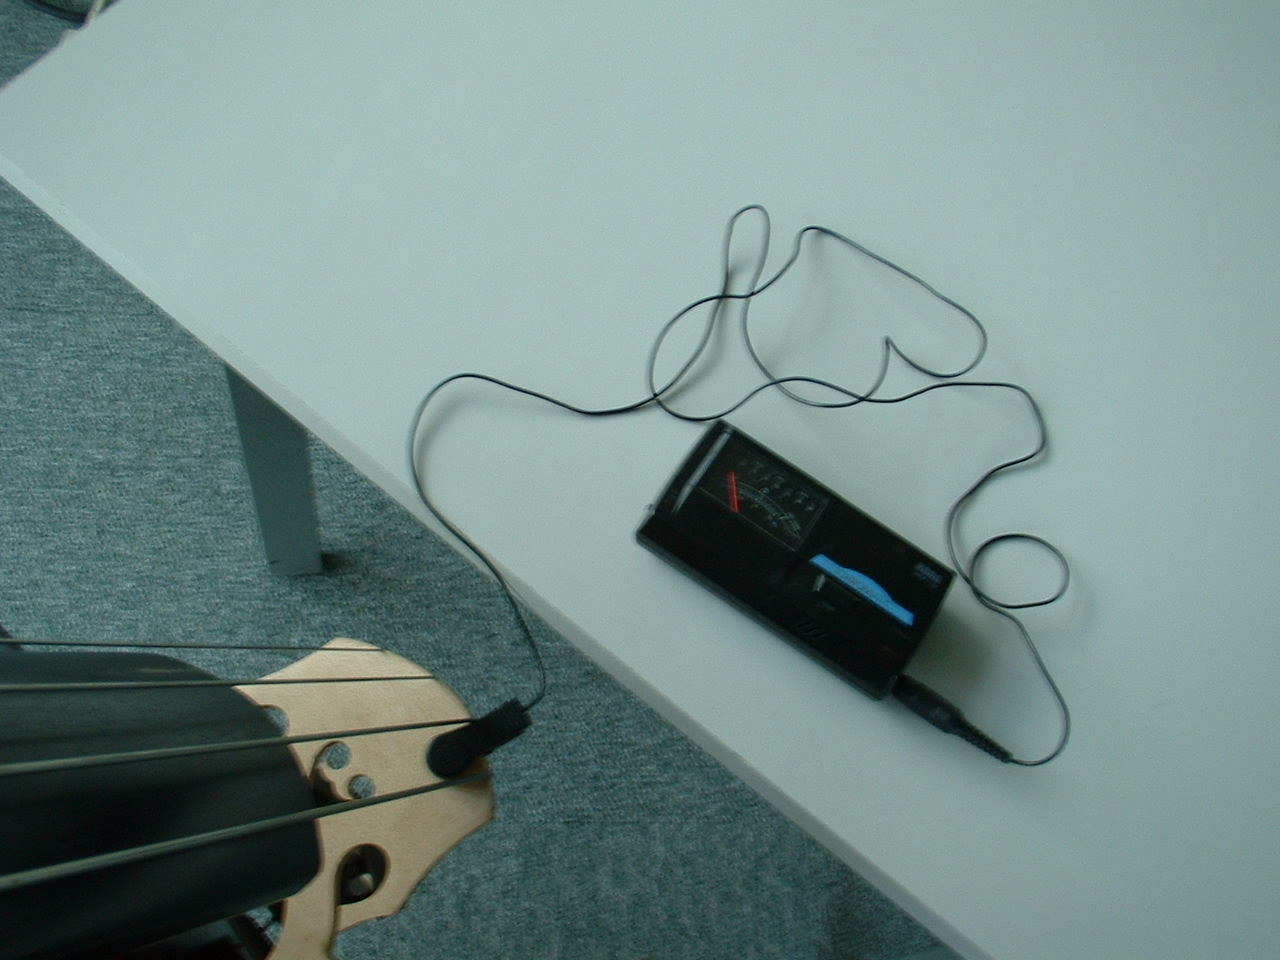
\includegraphics[width=4cm]{Pics/newphoto/contact2.epsi}\\
{\small 図\thefigure : マイクを駒にはさむ\\}
\end{center}
\end{minipage}
\end{flushleft}

\subsection{ボウイング(英: bowing)の記号}
\addtocounter{figure}{1}
\begin{center}
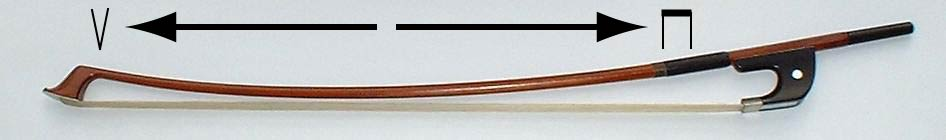
\includegraphics[width=12.5cm]{Pics/Bow/updown_bow.epsi}\\
{\small 図\thefigure : ボウイング記号とその示す方向\\}
\end{center}

\begin{center}
\begin{music}
\downbow 
\end{music}
\ \ \ \(\cdots\) ダウン・ボウ(通称「ダウン」)。弓を手元の方向へ動かします。

\begin{music}
\upbow 
\end{music}
\ \ \ \(\cdots\) アップ・ボウ(通称「アップ」)。弓を弓先の方向へ動かします。
\end{center}

小節の頭など強拍のところはダウン・ボウで弾く場合が多数です。逆に弱拍の音符はアップ・ボウで弾くのが一般的です。

\subsection{開放弦の練習 \label{open1}}
\begin{flushleft}
\begin{minipage}{310pt}
\ \ \ \ 調弦が終わったら、下の譜例\cite[pp.7]{simandl}を用いて開放弦で
音を鳴らす練習をしてみましょう。\underline{\bf 音量が均一になるように} 
気を配って下さい。また、今後はどんな練習をするときにも必ずメトロノーム
を使いましょう。オーケストラにおいてコントラバスは打楽器に次ぐ重要なリ
ズム楽器ですので、日頃からリズム感を磨いておきます。電子音でリズムを示
すものよりも打撃音でリズムを教えてくれるぜんまい式メトロノームの方が音
の通りが良く使いやすいでしょう。\\
\end{minipage}
\hfill
\begin{minipage}{120pt}
\addtocounter{figure}{1}
\begin{center}
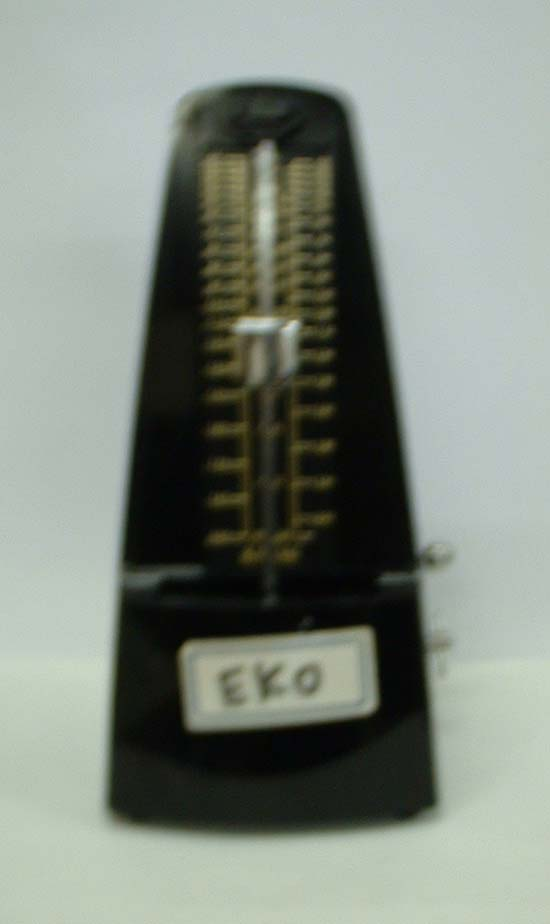
\includegraphics[height=4cm]{Pics/newphoto/metronome.epsi}\\
{\small 図\thefigure : ぜんまい式メトロノーム\\}
\end{center}
\end{minipage}
\end{flushleft}

\begin{music}
\nostartrule
\parindent 0pt
\setclef1{\bass}  
\generalmeter{\meterC}
\startpiece
\notes\zchar{14}{(\metron{\qu}{60})}\enotes
\NOtes\zchar{9}{\downbow}\wh{'D}\enotes
\bar
\notes\enotes
\NOtes\zchar{9}{\upbow}\wh{'A}\enotes
\bar
\notes\enotes
\NOtes\wh{'D}\enotes
\bar
\notes\enotes
\NOtes\wh{'G}\enotes
\bar
\notes\enotes
\NOtes\wh{'A}\enotes
\bar
\notes\enotes
\NOtes\wh{'D}\enotes
\bar
\notes\enotes
\NOtes\wh{E}\enotes
\bar
\notes\enotes
\NOtes\wh{'A}\enotes
\endpiece

\startpiece
\notes\enotes
\Notes\zchar{9}{\downbow}\hl{'D}\zchar{9}{\upbow}\hl{D}\enotes
\bar
\Notes\hu{'A}\hu{A}\enotes
\bar
\Notes\hl{'D}\hl{D}\enotes
\bar
\Notes\hl{'G}\hl{G}\enotes
\bar
\Notes\hu{'A}\hu{A}\enotes
\bar
\Notes\hl{'D}\hl{D}\enotes
\bar
\Notes\hu{E}\hu{E}\enotes
\bar
\Notes\hu{'A}\hu{A}\enotes
\endpiece

\startpiece
\notes\zchar{9}{\downbow}\ql{'D}\zchar{9}{\upbow}\ql{DDD}\enotes
\bar
\notes\qu{'AAAA}\enotes
\bar
\notes\ql{'DDDD}\enotes
\bar
\notes\ql{'GGGG}\enotes
\bar
\notes\qu{'AAAA}\enotes
\bar
\notes\ql{'DDDD}\enotes
\bar
\notes\qu{EEEE}\enotes
\bar
\notes\qu{'AAAA}\enotes
\rightrepeat
\Notes\wh{'D}\enotes
\setdoublebar
\endpiece
\end{music}

\subsection{移弦 \label{strchg}}

\begin{minipage}{230pt}
\ \ \ \ 「\ref{open1}」の開放弦の練習をしてみて、音符と音符との間に音
が鳴っていない時間ができてしまいませんでしたか? もしそうなら、その理由
の1つは弦から弦への弓の移動(移弦)が滑らかでないことです。図
\addtocounter{figure}{1}\thefigure は、D線を弾いている弓の軌道を、徐々
に移動先のA線に近い軌道に移す様子を示しています。図中の数字は以下の弓
の軌道に対応します。

\begin{enumerate}
\item D線を弾く際の基本的な軌道
\item D線を弾きながらA線にぎりぎりまで近付く
\item A線に移った直後の軌道。この状態からA線を弾き始める。
\item A線を弾く際の基本的な軌道に移る
\end{enumerate}

図\addtocounter{figure}{1}\thefigure 、図\addtocounter{figure}{1}\thefigure は移弦の際の右手の動きを示しています。\\
\end{minipage}
\hfill
\begin{minipage}{180pt}
\begin{center}
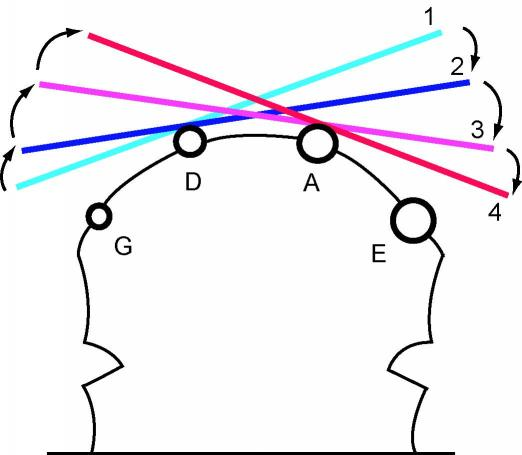
\includegraphics[height=5cm]{Pics/photo0830/strchg6.epsi}\\
\addtocounter{figure}{-2}
{\small 図\thefigure : D線からA線への移弦(1\(\rightarrow\)2\(\rightarrow\)3\(\rightarrow\)4)\\}
\end{center}
\end{minipage}

\begin{minipage}{200pt}
\begin{center}
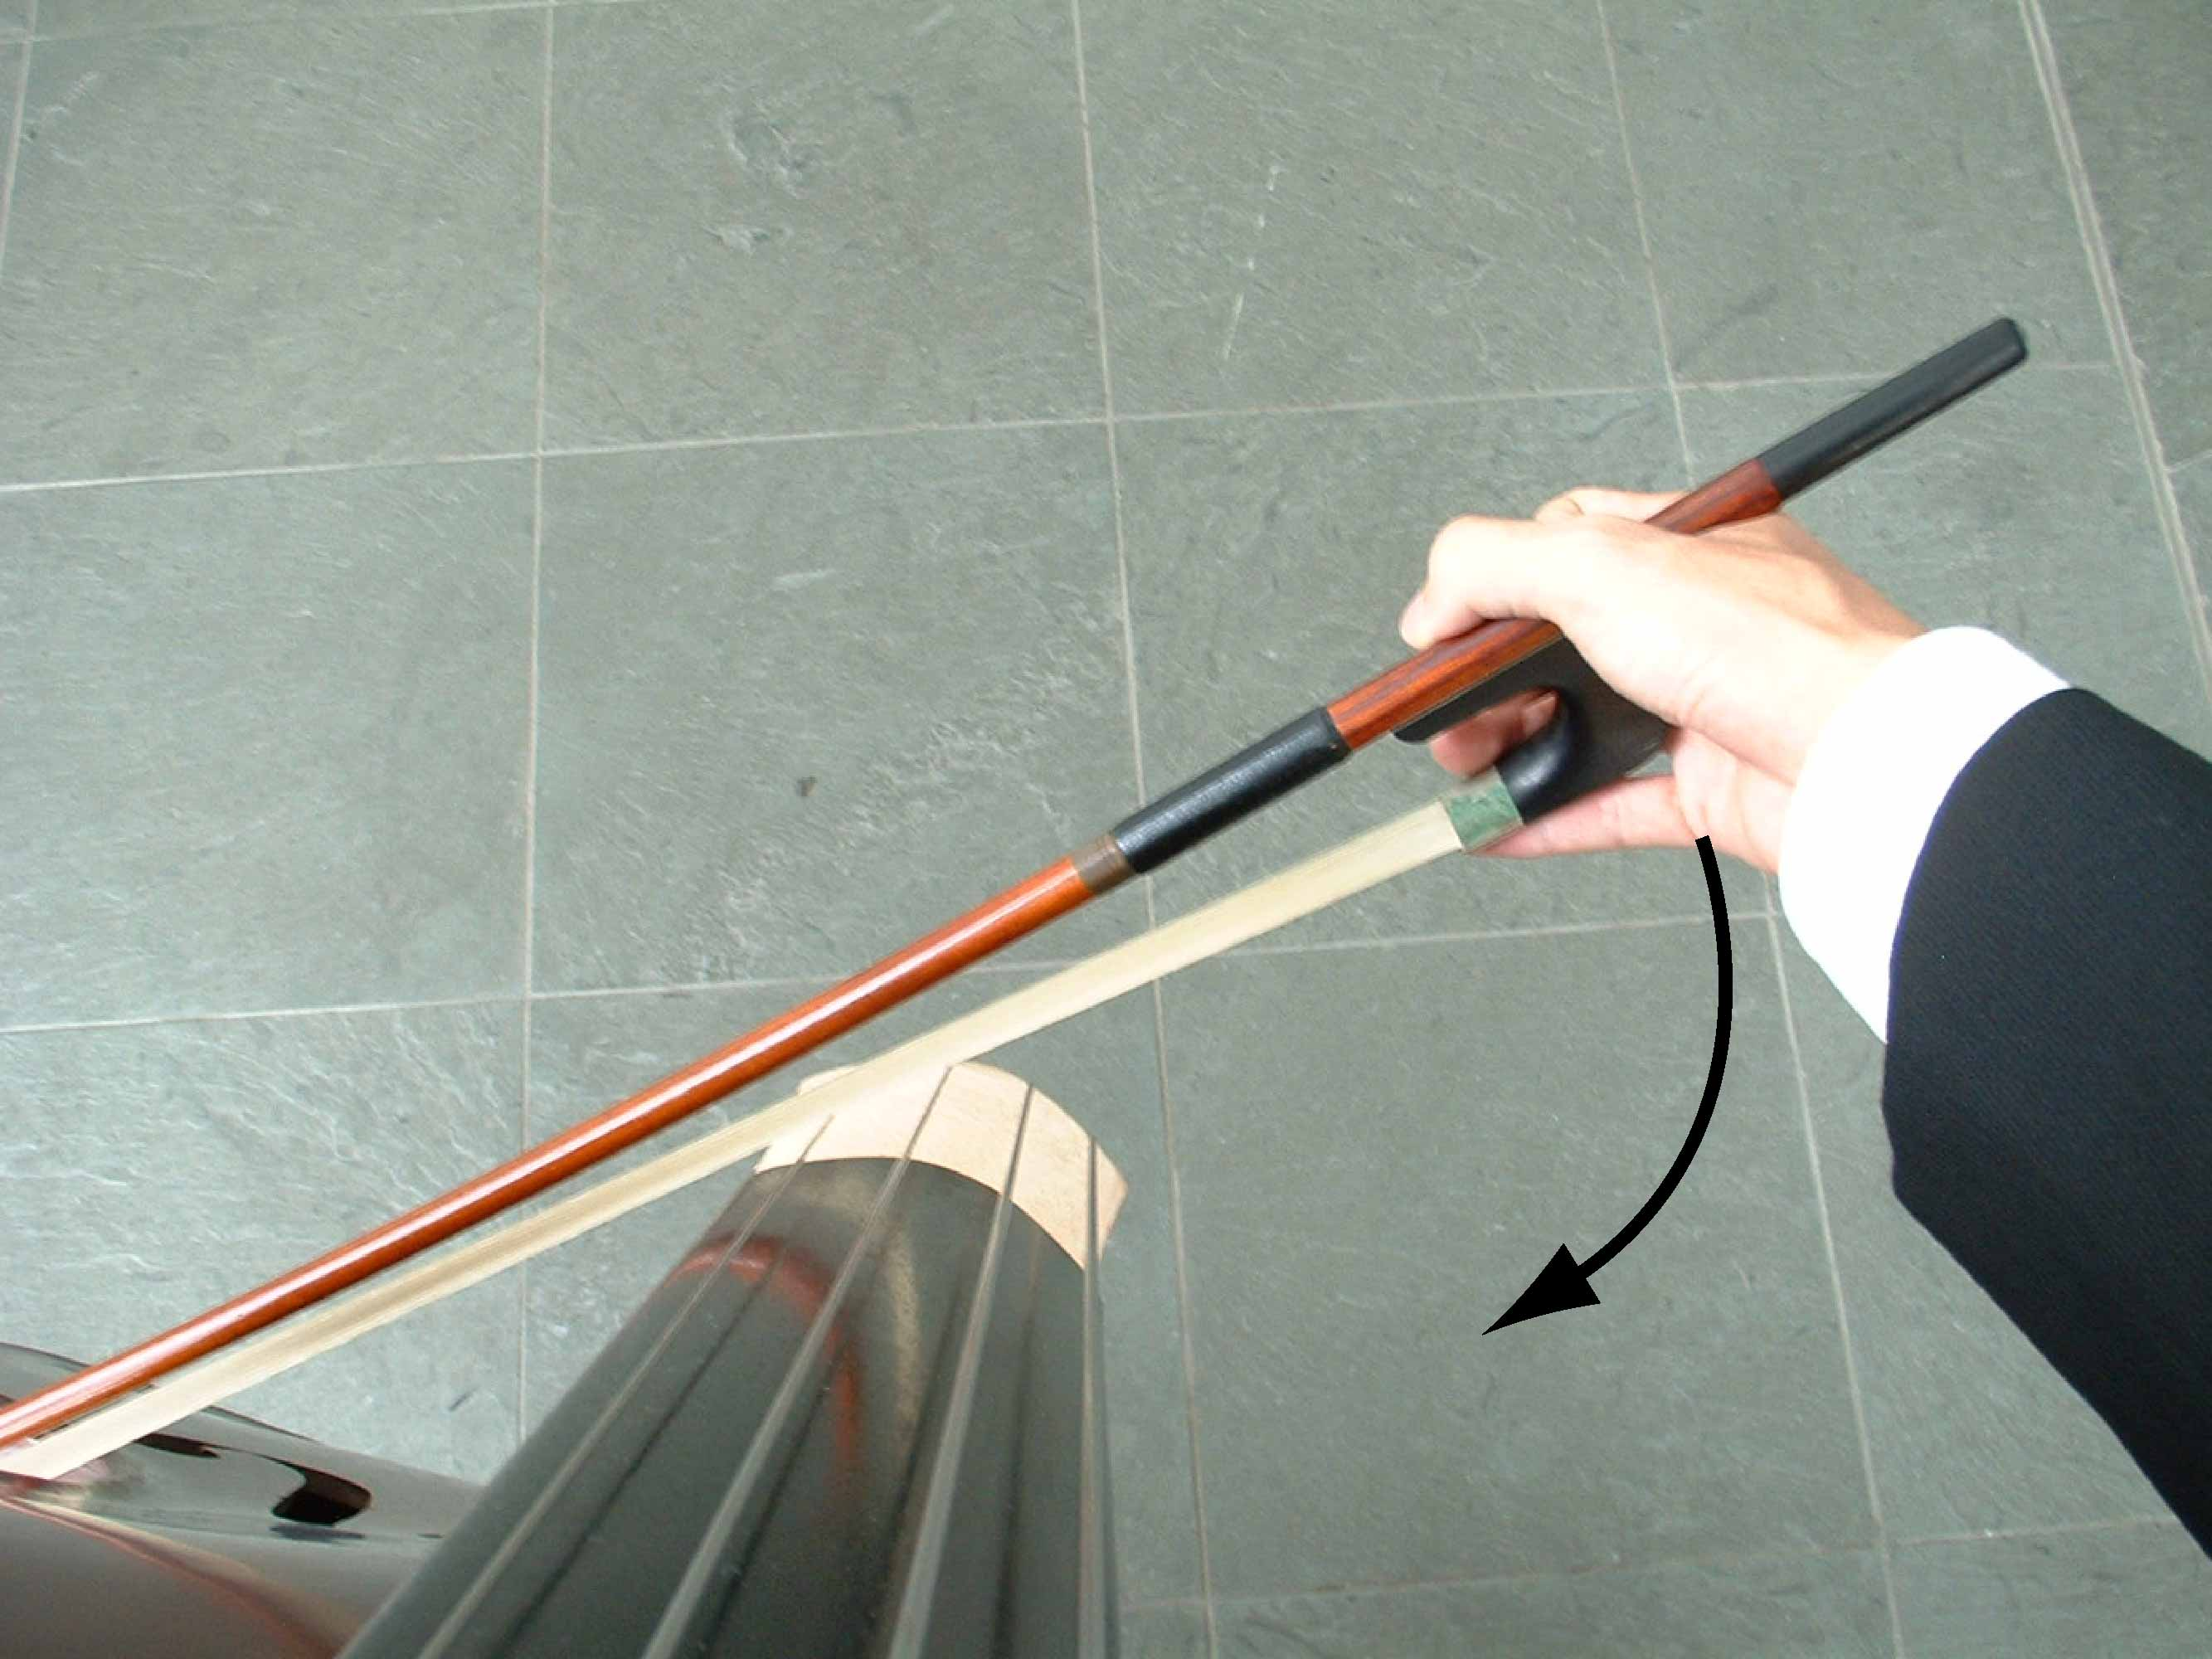
\includegraphics[height=3.8cm]{Pics/photo0830/strchg1.epsi}\\
\addtocounter{figure}{1}
{\small 図\thefigure : 手首を矢印の方向に持って行く\\}
\end{center}
\end{minipage}
\hfill
\begin{minipage}{200pt}
\begin{center}
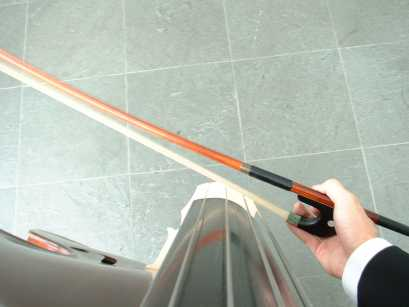
\includegraphics[height=3.8cm]{Pics/photo0830/strchg4.epsi}\\
\addtocounter{figure}{1}
{\small 図\thefigure : 移弦完了\\}
\end{center}
\end{minipage}

\subsection{手首の使い方 \label{wrist}}
音符と音符の間に隙間ができるもう1つの理由に、弓の折り返しがあります。弦上を動きだした弓はやがて末端(弓先か弓元)にたどり着きます。弾き続けるためにはここで折り返して、それまで弓が動いていた方向と逆の方向に弓を動かす必要があります。こうした弓の往復運動を円滑に行う際に重要なのが右手首の動きです。ダウン・ボウからアップ・ボウに移行するには以下のようにします。\\

\begin{quote}
\begin{enumerate}
\item ダウン・ボウで弾き始める
\item 弓先に近付く(図\addtocounter{figure}{1}\thefigure )
\item ダウン・ボウで弾き続けながら手首を内側に向かって突き出す(図\addtocounter{figure}{1}\thefigure )
\item 弓先に到達
\item アップ・ボウ動作の開始
\end{enumerate}
\end{quote}
\ \\
\begin{minipage}{200pt}
\addtocounter{figure}{-1}
\begin{center}
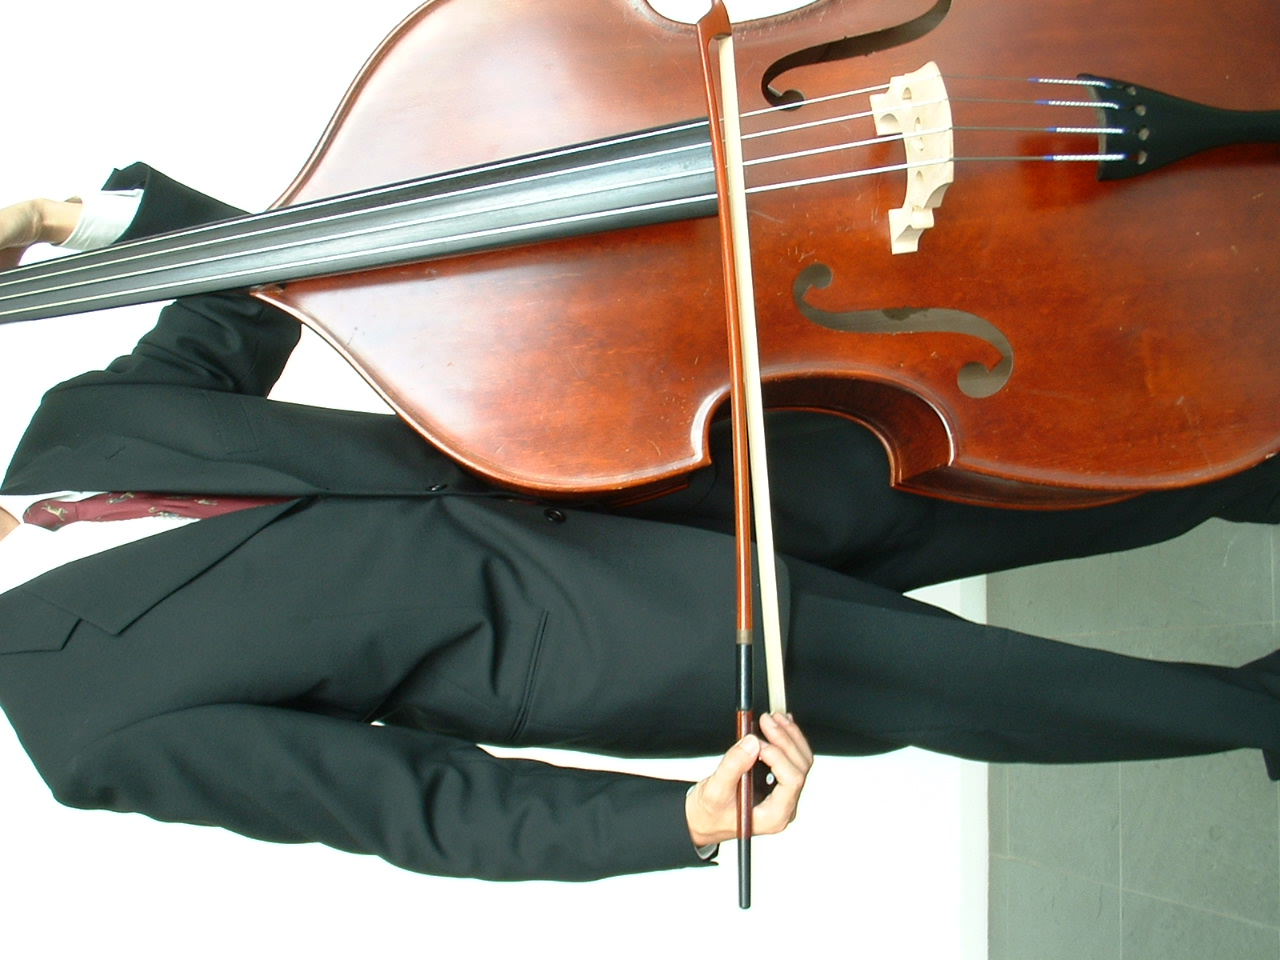
\includegraphics[height=6cm]{Pics/newphoto/bowing1.epsi}\\
{\small 図\thefigure : 弓先が近付く\\}
\end{center}
\end{minipage}
\hfill
\begin{minipage}{200pt}
\addtocounter{figure}{1}
\begin{center}
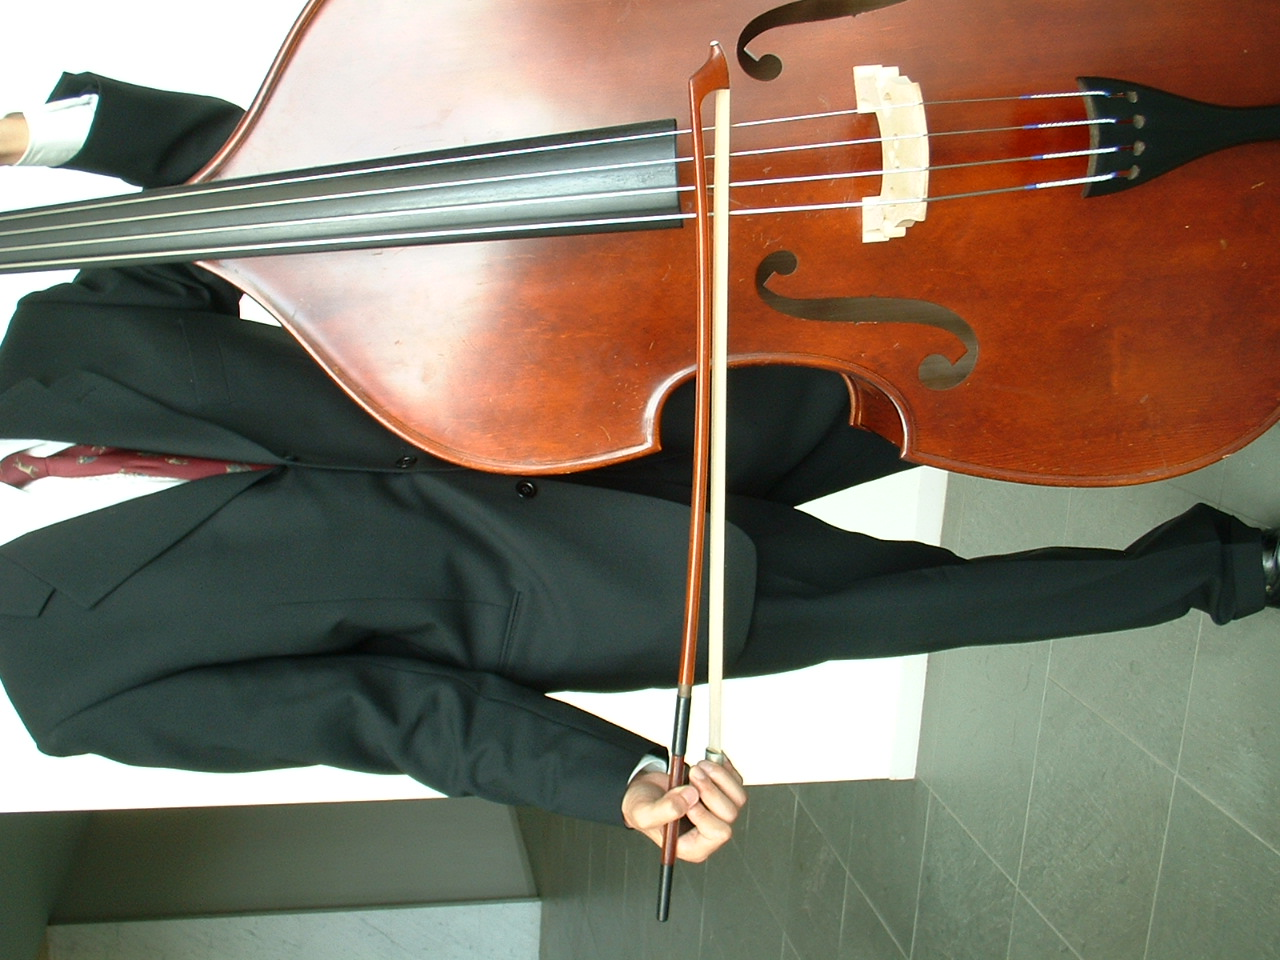
\includegraphics[height=6cm]{Pics/newphoto/bowing2.epsi}\\
{\small 図\thefigure : 手首を内側に入れる\\}
\end{center}
\end{minipage}

\ \\
\indent 逆にアップ・ボウからダウン・ボウに移行するには次のようにします。

\begin{quote}
\begin{enumerate}
\item アップ・ボウで弾き始める
\item 弓元に近付く(図\addtocounter{figure}{1}\thefigure )
\item アップ・ボウで弾き続けながら、内側に突き出していた手首をゆっくり戻す(図\addtocounter{figure}{1}\thefigure )
\item 弓元に到達
\item ダウン・ボウ動作の開始
\end{enumerate}
\end{quote}

\begin{minipage}{200pt}
\addtocounter{figure}{-1}
\begin{center}
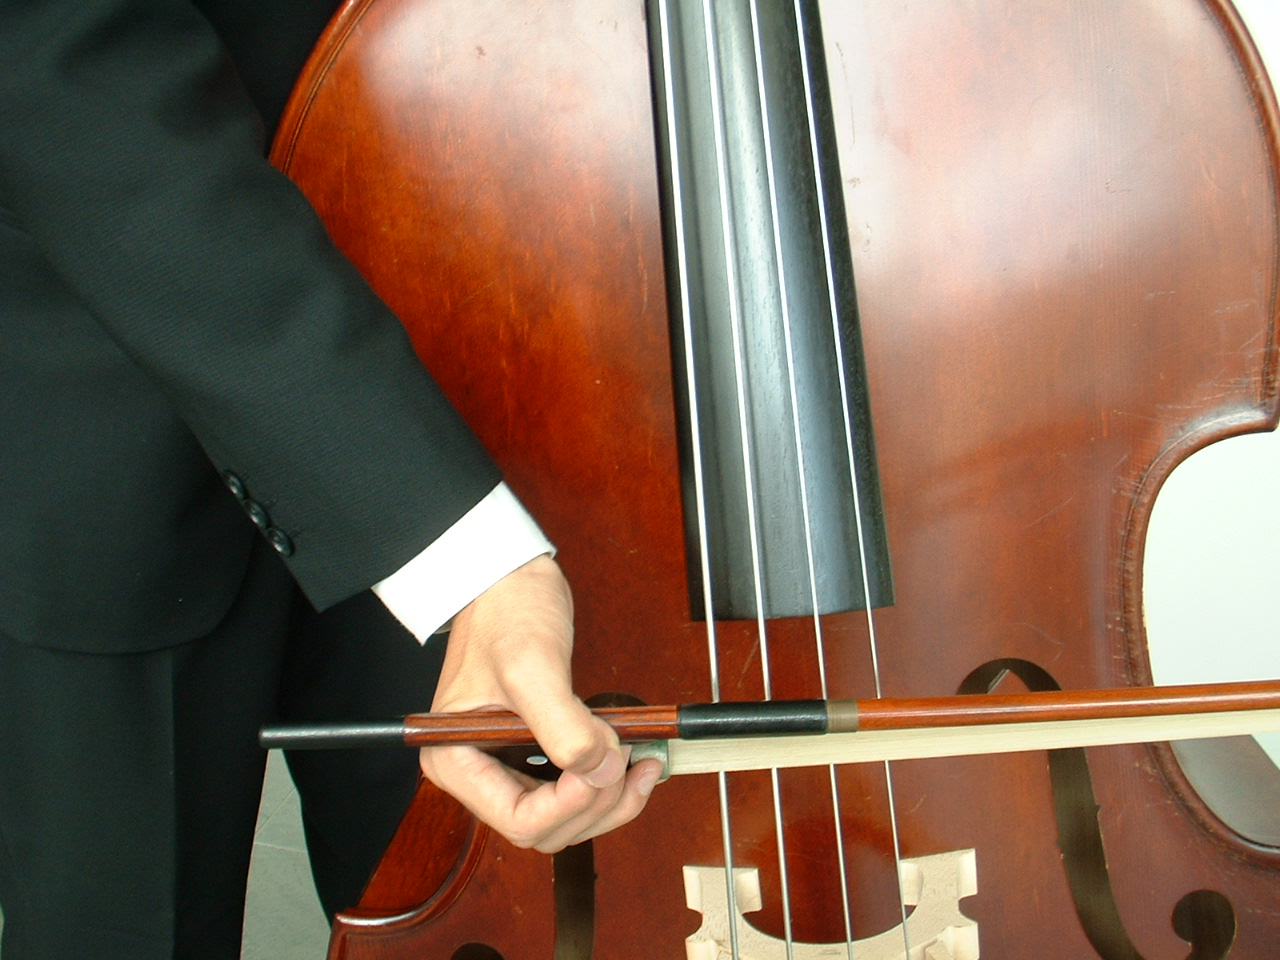
\includegraphics[height=5.4cm]{Pics/newphoto/bowing4.epsi}\\
{\small 図\thefigure : 弓元が近付く\\}
\end{center}
\end{minipage}
\hfill
\begin{minipage}{200pt}
\addtocounter{figure}{1}
\begin{center}
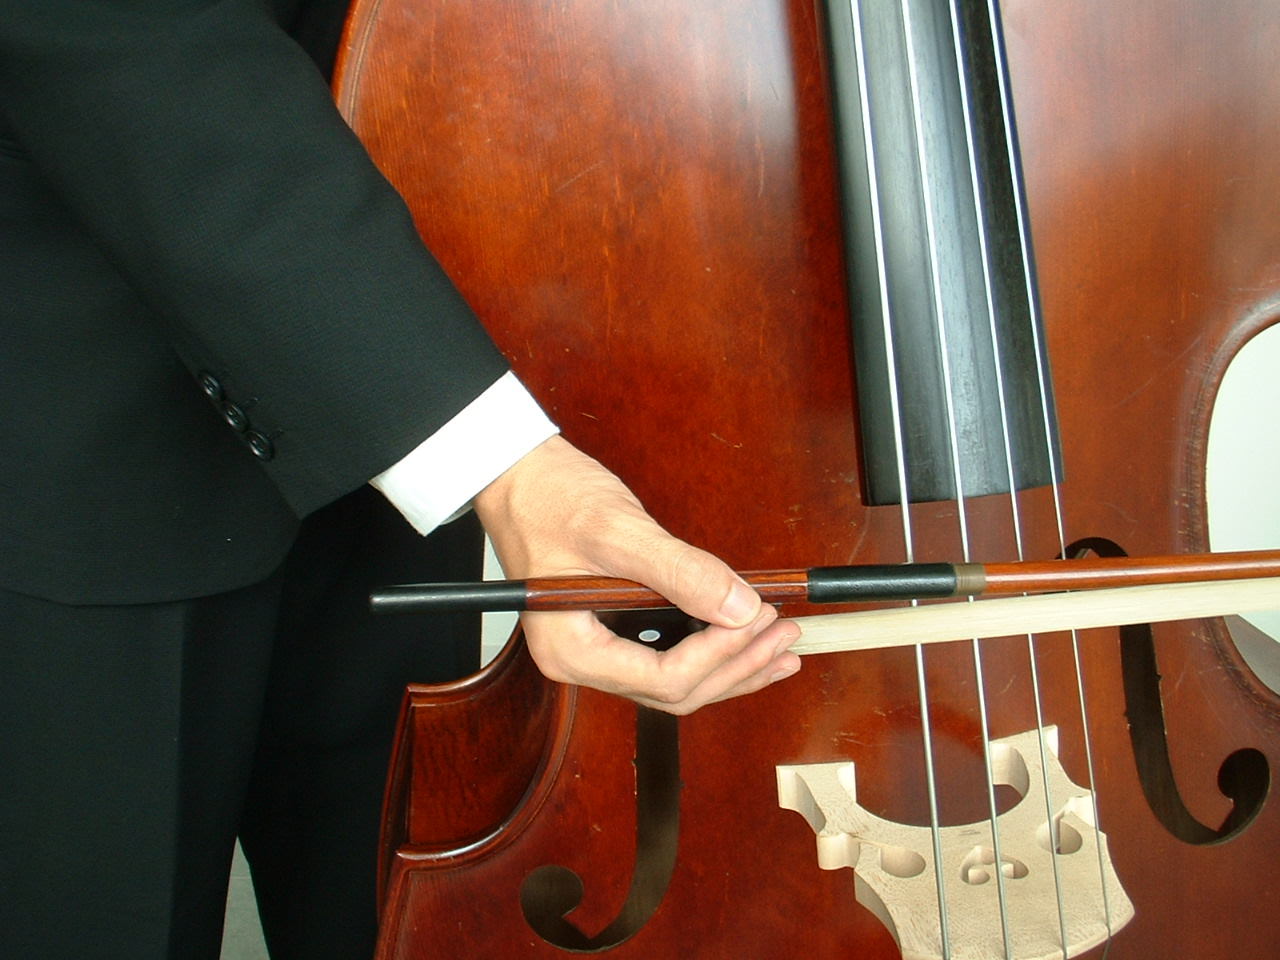
\includegraphics[height=5.4cm]{Pics/newphoto/bowing3.epsi}\\
{\small 図\thefigure : 内側に突き出していた手首を戻す\\}
\end{center}
\end{minipage}

\ \\

最初のうちは弓を折り返した際に弦の振動が止まるか減衰してしまうと思いま
すが、習得に比較的時間がかかる技術ですので焦る必要はありません。毎日の
基礎練習の中で少しずつ取り組んで下さい。弓を折り返しても弦の振動が持続
できるまでになれば、弓の円滑な往復運動をマスターしたと言えるでしょう。

\clearpage

\subsection{開放弦の練習 \label{open2}}
「\ref{strchg}」「\ref{wrist}」で紹介した移弦の方法、手首の使い方を踏
まえて、音符と音符との間に音が鳴っていない時間ができないように開放弦の
練習をしてみましょう。今後、開放弦の練習をするときには、必ず以下の3項
目を点検しながら練習するようにします。

\begin{enumerate}
\item 音量は均一か
\item 手首が柔らかく動いているか
\item 音符の間に音が鳴っていない時間はないか
\end{enumerate}

\begin{music}
\nostartrule
\parindent 0pt
\setclef1{\bass}  
\generalmeter{\meterC}
\startpiece
\notes\zchar{14}{(\metron{\qu}{60})}\enotes
\NOtes\zchar{9}{\downbow}\wh{'D}\enotes
\bar
\notes\enotes
\NOtes\zchar{9}{\upbow}\wh{'A}\enotes
\bar
\notes\enotes
\NOtes\wh{'D}\enotes
\bar
\notes\enotes
\NOtes\wh{'G}\enotes
\bar
\notes\enotes
\NOtes\wh{'A}\enotes
\bar
\notes\enotes
\NOtes\wh{'D}\enotes
\bar
\notes\enotes
\NOtes\wh{E}\enotes
\bar
\notes\enotes
\NOtes\wh{'A}\enotes
\endpiece

\startpiece
\notes\enotes
\Notes\zchar{9}{\downbow}\hl{'D}\zchar{9}{\upbow}\hl{D}\enotes
\bar
\Notes\hu{'A}\hu{A}\enotes
\bar
\Notes\hl{'D}\hl{D}\enotes
\bar
\Notes\hl{'G}\hl{G}\enotes
\bar
\Notes\hu{'A}\hu{A}\enotes
\bar
\Notes\hl{'D}\hl{D}\enotes
\bar
\Notes\hu{E}\hu{E}\enotes
\bar
\Notes\hu{'A}\hu{A}\enotes
\endpiece

\startpiece
\notes\zchar{9}{\downbow}\ql{'D}\zchar{9}{\upbow}\ql{DDD}\enotes
\bar
\notes\qu{'AAAA}\enotes
\bar
\notes\ql{'DDDD}\enotes
\bar
\notes\ql{'GGGG}\enotes
\bar
\notes\qu{'AAAA}\enotes
\bar
\notes\ql{'DDDD}\enotes
\bar
\notes\qu{EEEE}\enotes
\bar
\notes\qu{'AAAA}\enotes
\rightrepeat
\Notes\wh{'D}\enotes
\setdoublebar
\endpiece
\end{music}

\begin{flushleft}
\begin{minipage}{200pt}
\subsection{ピッツィカート(伊 pizzicato)}
\ \ \ \ 譜面上にpizz.と書いてあったら、それ以降の音符は右手の指で弦を
はじいて演奏します。これをピッツィカート奏法と呼びます。ピッツィカート
はarcoと書かれている地点まで続きます。arco以降は元通り弓で演奏します。
強いピッツィカート音を出したいときは人さし指と中指の2本で、小さい音が
欲しいときは人さし指1本ではじきます。
\end{minipage}
\hfill
\begin{minipage}{60pt}
\begin{center}
\addtocounter{figure}{1}
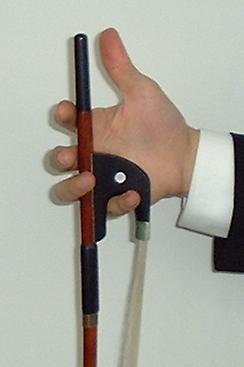
\includegraphics[height=4.5cm]{Pics/Pizz/pizz_1.epsi}\\
図\thefigure \\
\end{center}
\end{minipage}
\hfill
\begin{minipage}{90pt}
\begin{center}
\addtocounter{figure}{1}
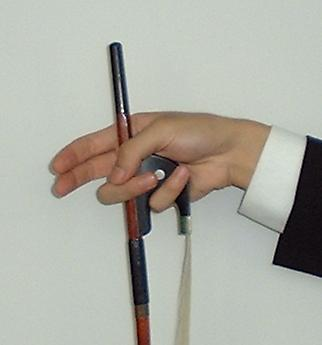
\includegraphics[height=4.5cm]{Pics/Pizz/pizz_2.epsi}\\
図\thefigure \\
\end{center}
\end{minipage}
\end{flushleft}

\begin{minipage}{100pt}
\begin{center}
\addtocounter{figure}{1}
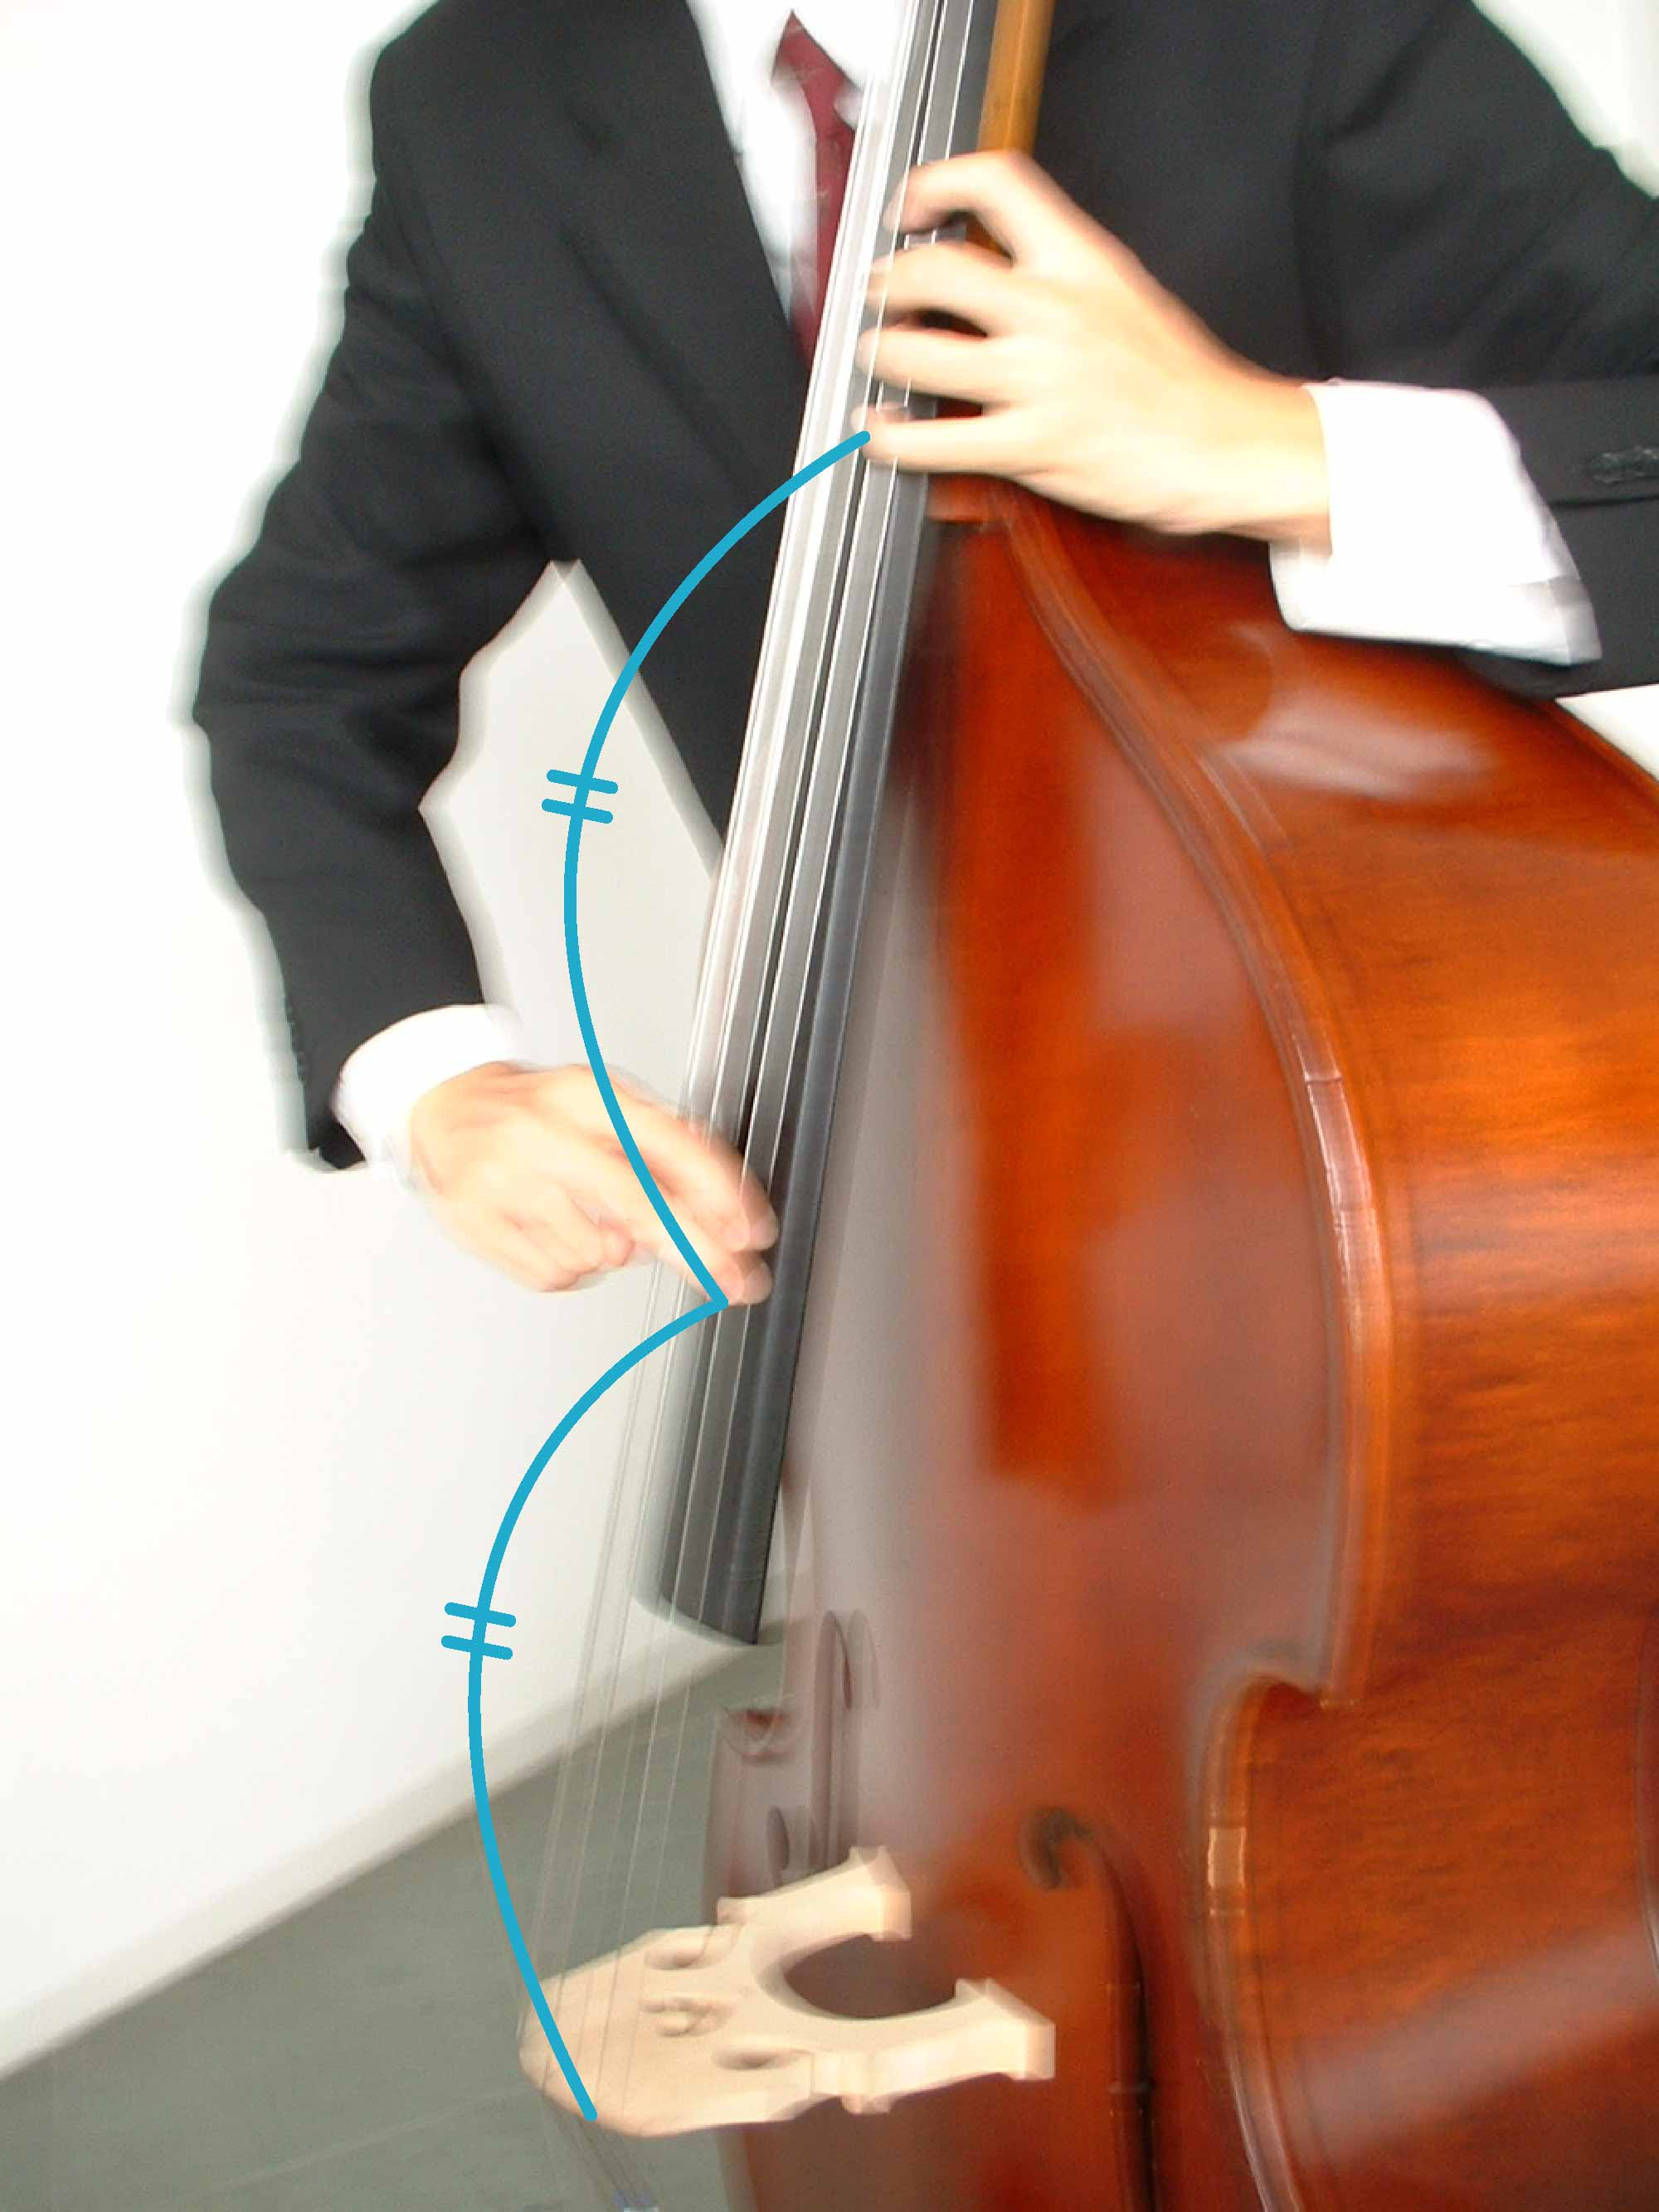
\includegraphics[height=4.5cm]{Pics/photo0830/pizz_point.epsi}\\
図\thefigure \\
\end{center}
\end{minipage}
\hfill
\begin{minipage}{100pt}
\begin{center}
\addtocounter{figure}{1}
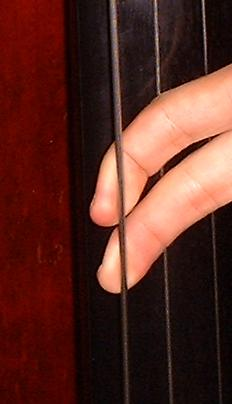
\includegraphics[height=4.5cm]{Pics/Pizz/pizz_3.epsi}\\
図\thefigure \\
\end{center}
\end{minipage}
\hfill
\begin{minipage}{220pt}
\begin{center}
\addtocounter{figure}{1}
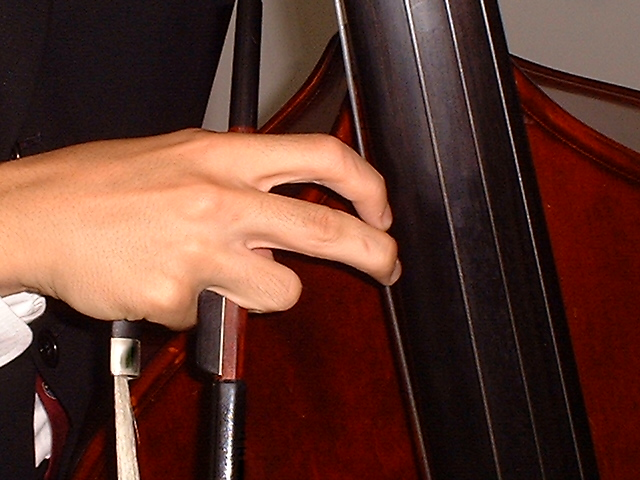
\includegraphics[height=4.5cm]{Pics/Pizz/pizz_4.epsi}\\
図\thefigure \\
\end{center}
\end{minipage}

\begin{enumerate}
\item まず小指に弓を引っ掛けます(\addtocounter{figure}{-4}図\thefigure )。
\item 弓を握ります(\addtocounter{figure}{1}図\thefigure )。
\item 左手で押さえた地点から駒までの中間点に右手の指を持って行きます(\addtocounter{figure}{1}図\thefigure )。
\item 指を弦に押し当て、指先に「肉溜まり」をつくります(\addtocounter{figure}{1}図\thefigure )。
\item 弦を横方向に引っ張ります(\addtocounter{figure}{1}図\thefigure )。
\item 弦を放し、エネルギーを一気に開放します。弦を指板に当てて雑音を出さないように注意しましょう。
\end{enumerate}

\subsection{ベース椅子とその座り方}

\begin{minipage}{200pt}
\ \ \ \ \ コントラバスは立っても座っても演奏できます。座って演奏する場合には
\addtocounter{figure}{1}図\thefigure のような「ベース椅子」または「バス椅子」と呼ばれる高椅子に座ります。ベース椅子に座る際には\addtocounter{figure}{1}図
\thefigure のように左足を踏み台にかけ、右足を伸ばします。

\addtocounter{figure}{-1}
\begin{center}
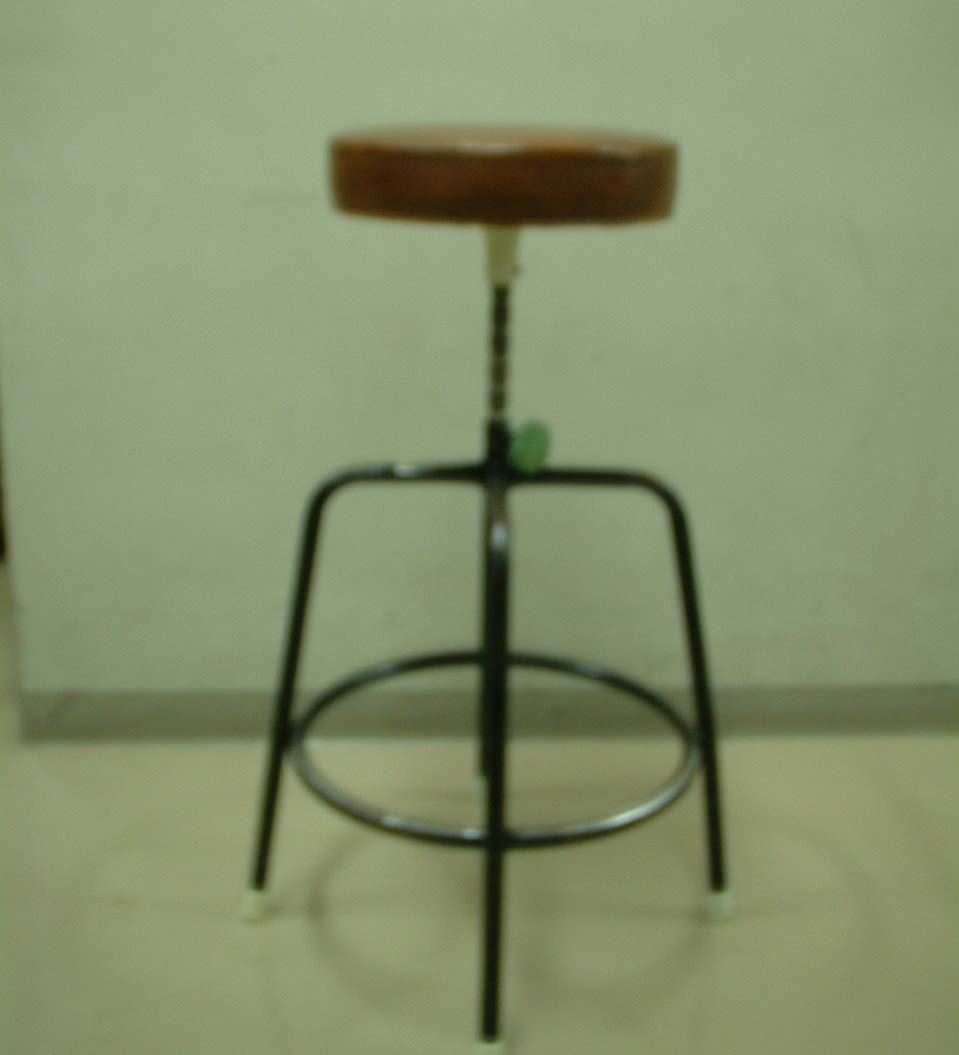
\includegraphics[width=2.3cm]{Pics/newphoto/chair1.epsi}\\
{\small 図\thefigure : 典型的なベース椅子\\}
\end{center}
\end{minipage}
\hfill
\begin{minipage}{120pt}
\addtocounter{figure}{1}
\begin{center}
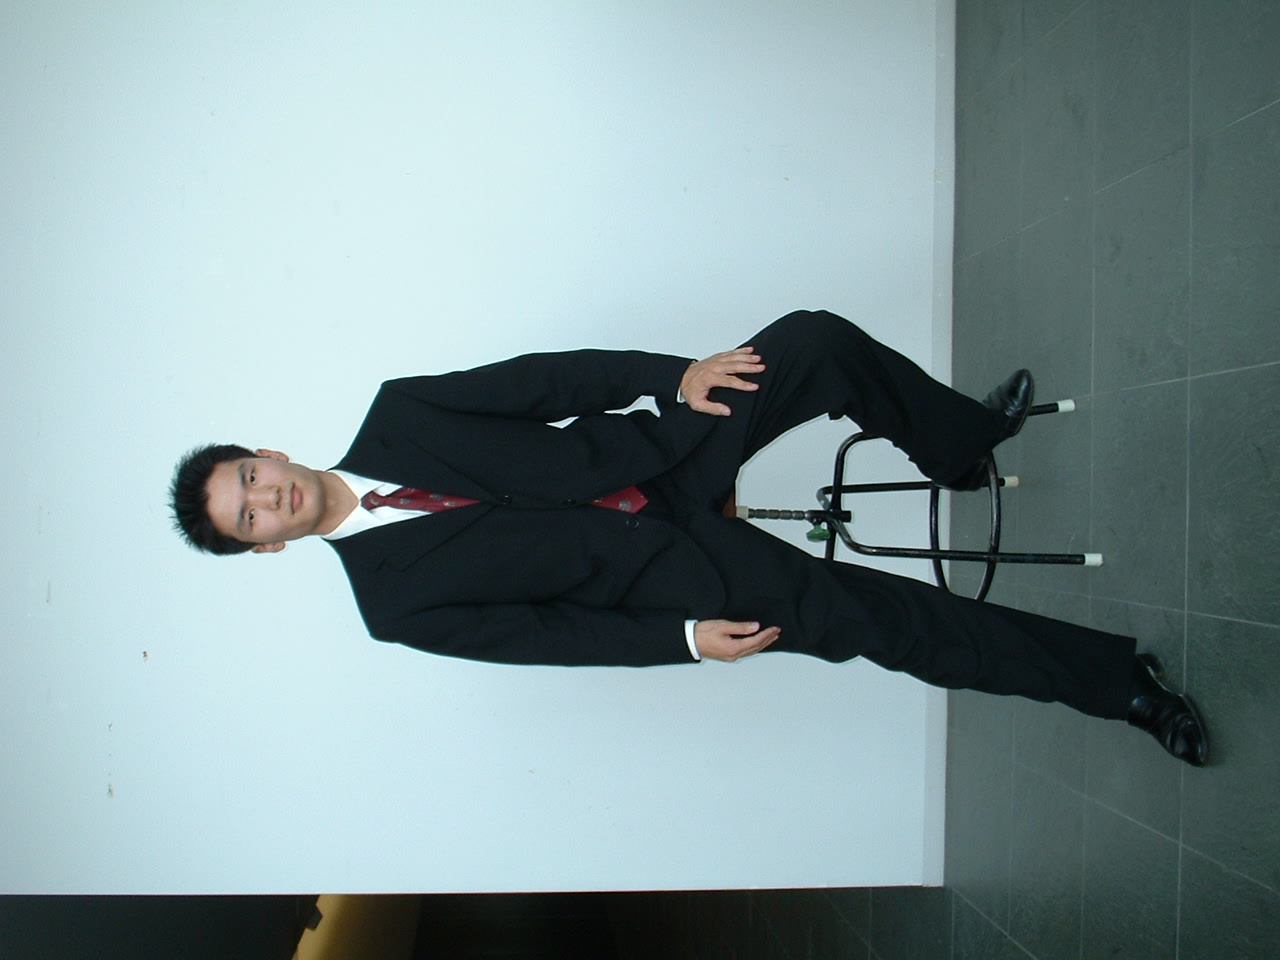
\includegraphics[height=6.5cm]{Pics/newphoto/chair2.epsi}\\
{\small 図\thefigure : 左足を踏み台にかける\\}
\end{center}
\end{minipage}
\hfill
\begin{minipage}{100pt}
\begin{center}
\includegraphics[height=6.5cm]{Pics/newphoto/chair3.epsi}\\
\addtocounter{figure}{1}
{\small 図\thefigure : 楽器を体に預ける\\}
\end{center}
\end{minipage}

\begin{minipage}{190pt}
\begin{center}
\includegraphics[height=5.8cm]{Pics/photo0830/sit_left.epsi}\\
\addtocounter{figure}{1}
{\small 図\thefigure : 左側から\\}
\end{center}
\end{minipage}
\hfill
\begin{minipage}{130pt}
\begin{center}
\includegraphics[height=5.8cm]{Pics/photo0830/sit_back.epsi}\\
\addtocounter{figure}{1}
{\small 図\thefigure : 背面から\\}
\end{center}
\end{minipage}
\hfill
\begin{minipage}{100pt}
\begin{center}
\includegraphics[height=5.8cm]{Pics/photo0830/sit_right.epsi}\\
\addtocounter{figure}{1}
{\small 図\thefigure : 右側から\\}
\end{center}
\end{minipage}


\clearpage

\clearpage
\section{左手のポジション}
\subsection{ポジションとは}
ネック上での左手の位置のことを{\bf ポジション}と言います(図\addtocounter{figure}{1} \thefigure)。コントラバスにはフレット\footnote{ギターの指板などに見られる、指で押さえる場所の目印となる直線状の突起}がありませんので、代わりに各ポジションの位置関係を身体感覚として身に付ける必要があります。これ以後の章ではポジションを1つずつ習得し、どの位置を押さえると何の音が出るのかを身体で覚えていきましょう。\\

\begin{flushleft}
\begin{minipage}{280pt}
\ \ \ \ 各ポジションはネックの上端から順に番号が振られています。本書では、ベーシストの間で広く認識されている\cite{simandl}のポジション番号に従います(下表参照)。シマンドルは1の指(人指し指)がA線上でイ短調自然短音階(A-H-C-D-E-F-G-A)の音を取るポジションに整数(I、II、III \(\cdots\) VII)を割り当て、それ以外を「中間ポジション」と名付けています。\\

\begin{small}
\begin{center}
表: 本書で使うポジション略記号\\ \ \\
\begin{tabular}{c|ll}
略記号 & \multicolumn{1}{c}{ポジション名} \cite{simandl} & \multicolumn{1}{c}{特徴}\\
\hline
h.p.   & ハーフ・ポジション       & ネックの上端にある\\
I      & 第Iポジション            & \\
II     & 第IIポジション            & \\
\(\roffset{0.6}{\small [}
\begin{tiny}
\begin{array}{c}
{\rm II}\\
{\rm III}\\
\end{array}
\end{tiny}
\)
 & 第II・第IIIの中間ポジション &\\
III    & 第IIIポジション      & 1と4がフラジオレット\\
\(\roffset{0.6}{\small [}
\begin{tiny}
\begin{array}{c}
{\rm III}\\
{\rm IV}\\
\end{array}
\end{tiny}
\)
& 第III・第IVの中間ポジション & \\
IV     & 第IVポジション            & ネックの根元にある\\
V      & 第Vポジション            & \\
\(\roffset{0.6}{\small [}
\begin{tiny}
\begin{array}{c}
{\rm V}\\
{\rm VI}\\
\end{array}
\end{tiny}
\)
& 第V・第VIの中間ポジション & 4の指はここまで\\
VI     & 第VIポジション            & 3の指がフラジオレット\\
\(\roffset{0.6}{\small [}
\begin{tiny}
\begin{array}{c}
{\rm VI}\\
{\rm VII}\\
\end{array}
\end{tiny}
\)
 & 第VI・第VIIの中間ポジション & \\
VII    & 第VIIポジション            & \\
\end{tabular}
\end{center}
\end{small}

\end{minipage}
\hfill
\begin{minipage}{140pt}
\begin{center}
\includegraphics[height=10cm]{Pics/Position/1st-4th.epsi}\\
{\flushleft\small 図\thefigure : 各ポジションの位置関係\\}
\end{center}
\end{minipage}
\end{flushleft}

\subsection{学習の順序}
通常、各ポジションの習得はネックの上端にあるハーフ・ポジションから開始し、徐々にネックの根元の方へと進んで行きます(手の位置が地面に近付くと弾ける音域は上がります)。しかし、ハーフ・ポジションは他のポジションにはない下記のような特徴があるため、
慣れるまではなにかと体力の要るポジションです。

\begin{enumerate}
\item 指の間を大きく広げる必要がある
\item 握力が要る
\item 腕を高い位置に保つ必要がある
\end{enumerate}

どれも慣れの問題なのですが、初心者には体力的なハードルであることは否めず、挫折の原因となりがちです。そこで本書では、比較的楽に握れる第IVポジションからスタートして、ネック上端のハーフ・ポジションへと進む順序で学習します。

%進める学習プログラムを用意しました。

%従来通りハーフ・ポジションから始める学習プログラムも併せて用意しましたので、自分に向いている方を選ぶことが可能です。\\

%ハーフ、第I、第II、第III、第IVの5ポジションの学習が終わったら、それ以降はどちらのコースでも共通の内容になります。

\clearpage
\section{第IVポジション}
\begin{center}
\begin{tabular}{|lcl|}
\hline
この章の基礎練習 & : & 開放弦の練習\\ 
この章の修了課題 & : & 1. 「\ref{half_scale}」の音階練習を正しい音程で暗譜して演奏できる\\
               &   & 2. ベートーヴェン、チャイコフスキー、「山の魔王の宮殿にて」からの抜粋を正しい音程で暗譜して演奏できる\\
\hline
\end{tabular}
\end{center}
\subsection{ベーシストの左手をつくる}
\begin{flushleft}
\begin{minipage}{203pt}
\ \ \ \ 左手の指には図\addtocounter{figure}{1}\thefigure のように番号が付いています。音符の上に書いてある数字に対応する指で弦を押さえます。例えば、4と書いてあったら小指で弦を押さえます。開放弦は0で表します。3の指は第\ref{6th}章ま
で使いません。\\
\end{minipage}
\hfill
\begin{minipage}{110pt}
\addtocounter{figure}{-1}
\begin{center}
\includegraphics[height=3.6cm]{Pics/Position/fingering.epsi}\\
{\small 図\thefigure : 指番号と縛る指\\}
\end{center}
\end{minipage}
\hfill
\begin{minipage}{120pt}
\addtocounter{figure}{1}
\begin{center}
\includegraphics[height=3.6cm]{Pics/photo0830/open_finger.epsi}\\
{\small 図\thefigure : ネックの根元に差し込む\\}
\end{center}
\end{minipage}
\end{flushleft}

左手の練習に入る前に、左手の2と3の指が離れないように縛ってください(図
\thefigure)。そして、1と2の間、2と4の間の距離が等しくなるように指を開
きます。左手の形が身に付くまでは図\thefigure のように指を縛ってから練
習します。比較的開きにくい1と2の指の間を広げるには、図
\addtocounter{figure}{1}\thefigure のようにネックの根元に指の間を差し
込むことを続けると有効です。\\

\subsection{第IVポジションの位置}
\begin{flushleft}
\begin{minipage}{160pt}
 最初に紹介する第IVポジションはネックの根元にあるポジションです(図
\addtocounter{figure}{2}\thefigure 、 
\addtocounter{figure}{1}\thefigure)。親指をネックの一番下まで降ろして
ください。その親指の正面を2の指で押さえます。これが第IVポジションです。
1と4は2に合わせます(図\addtocounter{figure}{1}\thefigure)。
\end{minipage}
\hfill
\begin{minipage}{80pt}
\addtocounter{figure}{-2}
\begin{center}
%\includegraphics[height=4.3cm]{Pics/Position/half_1.epsi}\\
\includegraphics[width=2cm]{Pics/now_printing.eps}\\
\end{center}
{\small 図\thefigure : 第IVポジションの位置\\}
\end{minipage}
\hfill
\begin{minipage}{80pt}
\addtocounter{figure}{1}
\begin{center}
\includegraphics[height=6.5cm]{Pics/Position/4th_2.epsi}\\
\end{center}
{\small 図\thefigure : 奏者から見た第IVポジション}\\
\end{minipage}
\hfill
\begin{minipage}{85pt}
\addtocounter{figure}{1}
\begin{center}
\includegraphics[height=4.3cm]{Pics/photo0830/left_thumb1.epsi}\\
\end{center}
{\small 図\thefigure : 左手親指の位置}\\
\end{minipage}
\end{flushleft}

\subsection{弦の押さえ方}
\indent 弦を押さえる際には1と2、2と4の指の間が均等に開くようにし、指の
先で押さえます(図\addtocounter{figure}{-2}\thefigure)。1の指はネックの
上側に少し傾け、指のやや側面寄りの位置で押さえます(図
\addtocounter{figure}{3}\thefigure)。 指は丸めてアーチ状にします(図
\thefigure)。図\addtocounter{figure}{1}\thefigure のようにつぶれたアー
チは正しくありません。
\begin{flushleft}
\begin{minipage}{220pt}
 また、2、4の指で押さえる場合には必ず上側の指も一緒に押さえます
(図\addtocounter{figure}{1}\thefigure)。たとえば2の指を押さえる際に
1を放してはいけません(図\addtocounter{figure}{1}\thefigure)。\\

\begin{minipage}{100pt}
\addtocounter{figure}{-3}
\begin{center}
\includegraphics[height=2cm]{Pics/newphoto/arch1.epsi}\\
\end{center}
{\small 図\thefigure : アーチ状に丸める。1は指の側面で押さえる。\\}
\end{minipage}
\hfill
\begin{minipage}{100pt}
\addtocounter{figure}{1}
\begin{center}
\includegraphics[height=2cm]{Pics/newphoto/arch2.epsi}\\
\end{center}
{\small 図\thefigure : アーチがつぶれてはダメ\\}
\end{minipage}
\end{minipage}
\hfill
\begin{minipage}{100pt}
\addtocounter{figure}{1}
\begin{center}
\includegraphics[width=3cm]{Pics/newphoto/finger1.epsi}\\
\end{center}
{\small 図\thefigure : 1の指も一緒に\\}
\end{minipage}
\hfill
\begin{minipage}{100pt}
\addtocounter{figure}{1}
\begin{center}
\includegraphics[width=3cm]{Pics/newphoto/finger2.epsi}\\
\end{center}
{\small 図\thefigure : 1を放してはダメ\\}
\end{minipage}
\end{flushleft}

\subsection{肘の位置}
\begin{flushleft}
\begin{minipage}{250pt}
 弦の押さえ方を覚えたら、次は肘の位置を習得しましょう。前腕(手首から肘まで)の角度が、ネックの上下方向と直角になる位置まで肘を上げます(図\addtocounter{figure}{1}\thefigure)。\\

\ \ \ \ 4の指は他の指と比べて押さえる力が弱いですが、このように肘を上げることで4の指の力を腕の重みで補えるようになります。
\end{minipage}
\hfill
\begin{minipage}{180pt}
\begin{center}
\includegraphics[height=4.5cm]{Pics/Shifting/orthogonal_halfsize.epsi}\\
図\thefigure : 腕とネックが直角になるのが目安\\
\end{center}
\end{minipage}
\end{flushleft}

\subsection{第IVポジションで取れる音}
第IVポジションではそれぞれの弦で以下の音を取ることができます。正し
い場所を押さえているかどうか、チューニングメーターで確認しながら弾いてみましょう。\\

\begin{music}
\nostartrule
\parindent 0pt
\setclef1{\bass}  
\startpiece
\notes\enotes
\Notes\zchar{18}{G線}\zchar{13}{\bf 1}\wh{d}\zchar{14}{\bf 2}\wh{^d}\zchar{14}{\bf 4}\wh{e}\enotes
\doublebar
\Notes\zchar{13}{\bf 1}\wh{d}\zchar{14}{\bf 2}\wh{_e}\zchar{14}{\bf 4}\wh{=e}\enotes
\doublebar
\Notes\zchar{18}{D線}\zchar{11}{\bf 1}\wh{a}\zchar{11}{\bf 2}\wh{^a}\zchar{11}{\bf 4}\wh{b}\enotes
\doublebar
\Notes\zchar{11}{\bf 1}\wh{a}\zchar{11}{\bf 2}\wh{_b}\zchar{11}{\bf 4}\wh{=b}\enotes
\setdoublebar
\endpiece
\startpiece
\notes\enotes
\Notes\zchar{14}{A線}\zchar{9}{\bf 1}\wh{'E}\zchar{9}{\bf 2}\wh{F}\zchar{9}{\bf 4}\wh{^F}\enotes
\doublebar
\Notes\zchar{9}{\bf 1}\wh{'E}\zchar{9}{\bf 2}\wh{F}\zchar{9}{\bf 4}\wh{_G}\enotes
\doublebar
\Notes\zchar{14}{E線}\zchar{9}{\bf 1}\wh{'B}\zchar{9}{\bf 2}\wh{C}\zchar{9}{\bf 4}\wh{^C}\enotes
\doublebar
\Notes\zchar{9}{\bf 1}\wh{'B}\zchar{9}{\bf 2}\wh{C}\zchar{9}{\bf 4}\wh{_D}\enotes
\setdoublebar
\endpiece
\end{music}

\subsection{音階練習 \label{half_scale}}
\begin{music}
\nostartrule
\parindent 0pt
\setclef1{\bass}  

\generalmeter{\meterC}
\generalsignature{0}    
\startpiece
\notes\zchar{14}{ハ長調(C-Dur)音階}\enotes
\NOtes\zchar{9}{\bf 2}\qu{'C}\zchar{9}{\bf 0}\ql{D}\zchar{9}{\bf 1}\ql{E}\zchar{9}{\bf 2}\ql{F}\enotes
\bar
\NOtes\zchar{9}{\bf 0}\ql{'G}\zchar{10}{\bf 1}\ql{!a}\zchar{11}{\bf 4}\ql{b}\qp\enotes
\bar
\NOtes\zchar{11}{\bf 4}\ql{b}\zchar{10}{\bf 1}\ql{a}\zchar{9}{\bf 0}\ql{'G}\zchar{9}{\bf 2}\ql{F}\enotes
\bar
\NOtes\zchar{9}{\bf 1}\ql{'E}\zchar{9}{\bf 0}\ql{D}\zchar{9}{\bf 2}\qu{C}\qp\enotes
\setdoublebar\endpiece

\generalmeter{\meterC}
\generalsignature{0}    
\startpiece
\notes\zchar{14}{イ短調(a-moll)音階}\enotes
\NOtes\zchar{9}{\bf 0}\qu{'A}\zchar{9}{\bf 1}\qu{B}\zchar{9}{\bf 2}\qu{C}\zchar{9}{\bf 0}\ql{D}\enotes
\bar
\NOtes\zchar{9}{\bf 1}\ql{'E}\zchar{9}{\bf 2}\ql{F}\zchar{10}{\bf 0}\ql{G}\zchar{11}{\bf 1}\ql{!a}\enotes
\bar
\NOtes\zchar{11}{\bf 1}\ql{a}\zchar{10}{\bf 0}\ql{'G}\zchar{9}{\bf 2}\ql{F}\zchar{9}{\bf 1}\ql{E}\enotes
\bar
\NOtes\zchar{9}{\bf 0}\ql{'D}\zchar{9}{\bf 2}\qu{C}\zchar{9}{\bf 1}\qu{B}\zchar{9}{\bf 0}\qu{A}\enotes
\setdoublebar\endpiece
\end{music}

\subsection{第IVポジションだけで弾ける名曲}
\subsubsection*{ワーグナー: 歌劇「さまよえるオランダ人」序曲より}
\begin{music}
\nostartrule
\setclef1{\bass}
\generalsignature{-1}    
\generalmeter{\meterfrac64}
\parindent 0pt
\startbarno=129
\def\writebarno{\tenrm\the\barno\barnoadd}
\def\raisebarno{2\internote}
\def\shiftbarno{0.1\Interligne}
\systemnumbers
\startpiece\bigaccid
\notes\zchar{18}{\bf Molto animato}\enotes
\Notes\zchar{12}{\upbow}\zchar{9}{\bf 0}\qu{'A}\zchar{-5}{\ff}\enotes
\bar
\Notes\zchar{-5}{\it marcato}\zchar{12}{\downbow}\zchar{9}{\bf 0}\hlp{'D}\zchar{9}{\upbow}\hl{D}\zchar{9}{\upbow}\qu{A}\enotes
\bar
\Notes\zchar{12}{\downbow}\zchar{9}{\bf 0}\hl{'D}\zchar{9}{\upbow}\ql{D}\zchar{15}{\downbow}\zchar{12}{\bf 1}\isluru{0}{!a}\hlp{a}\enotes\barno=130
\bar
\Notes\tslur{0}{a}\hl{a}\zchar{12}{\upbow}\zchar{9}{\bf 0}\ql{'D}\zchar{9}{\downbow}\hl{D}\zchar{9}{\upbow}\ql{D}\enotes
\bar
\Notes\zchar{17}{\downbow}\zchar{14}{\bf 1}\isluru{0}{d}\whp{d}\enotes
\bar
\Notes\tslur{0}{d}\ql{d}\zchar{12}{\upbow}\zchar{9}{\bf 0}\ql{'D}\zchar{9}{\downbow}\ql{D}\zchar{9}{\upbow}\ql{D}\zchar{9}{\downbow}\ql{D}\zchar{9}{\upbow}\ql{D}\enotes
\bar
\Notes\zchar{12}{\downbow}\zchar{9}{\bf 0}\ql{'G}\enotes
\setdoublebar
\endpiece
\end{music}

\documentclass{jarticle}
\usepackage{musixdoc}
\startmuflex\makeindex

\begin{document}

\subsubsection*{�쥹�ԡ���: ������֥����ޤξ��פ��֥���������ն�ξ���}
\begin{music}
\nostartrule
\setclef1{\bass}
\generalsignature{1}    
\generalmeter{\meterfrac54}
\parindent 0pt
\startbarno=28
\def\writebarno{\tenrm\the\barno\barnoadd}
\def\raisebarno{2\internote}
\def\shiftbarno{0.1\Interligne}
\systemnumbers
\startpiece\bigaccid
\notes\zchar{18}{\bf Ancora pi\`{u} mosso (\metron{\qu}{69})}\enotes
\notes\ibl{0}{b}{0}\ibbl{0}{b}{0}\qb{0}{b}\qb{0}{b}\qb{0}{b}\tbbl{0}\tbl{0}\qb{0}{b}\enotes
\notes\ibl{0}{b}{-2}\ibbl{0}{b}{-2}\qb{0}{b}\qb{0}{b}\qb{0}{b}\tbbl{0}\tbl{0}\qb{0}{a}\enotes
\notes\ibl{0}{b}{0}\ibbl{0}{b}{0}\qb{0}{b}\qb{0}{b}\qb{0}{d}\tbbl{0}\tbl{0}\qb{0}{b}\enotes
\notes\ibl{0}{b}{-2}\qb{0}{b}\ibbl{0}{b}{-2}\qb{0}{a}\tbbl{0}\tbl{0}\qb{0}{a}\enotes
\Notes\ql{b}\enotes
\bar
\Notes\hlp{b}\hl{b}\enotes
\bar
\notes\ibl{0}{b}{0}\ibbl{0}{b}{0}\qb{0}{b}\qb{0}{b}\qb{0}{b}\tbbl{0}\tbl{0}\qb{0}{b}\enotes
\notes\ibl{0}{b}{-2}\ibbl{0}{b}{-2}\qb{0}{b}\qb{0}{b}\qb{0}{b}\tbbl{0}\tbl{0}\qb{0}{a}\enotes
\notes\ibl{0}{b}{0}\ibbl{0}{b}{0}\qb{0}{b}\qb{0}{b}\qb{0}{d}\tbbl{0}\tbl{0}\qb{0}{b}\enotes
\notes\ibl{0}{b}{-2}\qb{0}{b}\ibbl{0}{b}{-2}\qb{0}{a}\tbbl{0}\tbl{0}\qb{0}{a}\enotes
\Notes\ql{b}\enotes
\bar
\Notes\hlp{b}\hl{b}\enotes
\bar
\notes\ibl{0}{b}{0}\ibbl{0}{b}{0}\qb{0}{b}\qb{0}{b}\qb{0}{b}\tbbl{0}\tbl{0}\qb{0}{b}\enotes
\notes\ibl{0}{b}{-2}\ibbl{0}{b}{-2}\qb{0}{b}\qb{0}{b}\qb{0}{b}\tbbl{0}\tbl{0}\qb{0}{a}\enotes
\notes\ibl{0}{b}{0}\ibbl{0}{b}{0}\qb{0}{b}\qb{0}{b}\qb{0}{d}\tbbl{0}\tbl{0}\qb{0}{b}\enotes
\notes\ibl{0}{b}{-2}\qb{0}{b}\ibbl{0}{b}{-2}\qb{0}{a}\tbbl{0}\tbl{0}\qb{0}{a}\enotes
\Notes\ql{b}\enotes 
\bar
\Notes\hlp{b}\hl{b}\enotes
\setdoublebar
\endpiece
\end{music}
\endmuflex
\end{document}

\subsubsection*{マーラー: 交響曲第1番 ニ長調 第2楽章より}

\begin{music}
\nostartrule
\setclef1{\bass}
\generalsignature{3}
\generalmeter{\meterfrac34}
\parindent 0pt
\def\writebarno{\tenrm\the\barno\barnoadd}
\def\raisebarno{2\internote}
\def\shiftbarno{0.1\Interligne}
\startbarno=285
\systemnumbers
\startpiece\bigaccid
\notes\zchar{17}{\Bigtype 26}\sk  \zchar{19}{\ \ \bf Tempo primo. (Kr\"{a}ftig bewegt, doch nicht zu schunell)}\enotes
\notes\loffset{1.5}{\zchar{-8}{\ff}}\zchar{12}\downbow\zchar{10}{\bf 1}\hl{a}\zchar{-5}{\bf 1}\sk\enotes
\Notes\zchar{12}\upbow\zchar{9}{\bf 1}\upz{'E}\ql{E}\enotes
\bar
\Notes\zchar{14}\downbow\zchar{11}{\bf 1}\upz{a}\ql{a}\zchar{14}\upbow\zchar{11}{\bf 1}\upz{a}\ql{a}\zchar{11}\upbow\zchar{8}{\bf 1}\upz{'E}\ql{E}\enotes
\bar
\notes\hl{a}\zchar{-5}{\bf 2}\sk\enotes
\Notes\upz{'E}\ql{E}\enotes
\bar
\Notes\upz{a}\ql{a}\upz{a}\ql{a}\upz{'E}\ql{E}\enotes
\bar
\notes\hl{a}\zchar{-5}{\bf 3}\sk\enotes
\Notes\upz{'E}\ql{E}\enotes
\bar
\Notes\upz{a}\ql{a}\upz{a}\ql{a}\upz{'E}\ql{E}\enotes
\bar
\notes\hl{a}\zchar{-5}{\bf 4}\sk\enotes
\Notes\upz{'E}\ql{E}\enotes
\bar
\Notes\upz{a}\ql{a}\upz{a}\ql{a}\zchar{-5}{\p}\upz{'E}\ql{E}\enotes
\bar
\notes\hl{a}\zchar{-5}{\bf 5}\sk\enotes
\Notes\upz{'E}\ql{E}\enotes
\bar
\Notes\upz{a}\ql{a}\upz{a}\ql{a}\zchar{-5}{\p}\upz{'E}\ql{E}\enotes
\bar
\notes\zchar{9}\downbow\hl{a}\sk\enotes
\Notes\zchar{9}\upbow\ql{'E}\enotes
\bar
\Notes\zchar{10}\downbow\upz{a}\ql{a}\zchar{10}\upbow\upz{a}\ql{a}\zchar{10}\downbow\upz{a}\ql{a}\enotes
\bar
\Notes\zchar{15}\upbow\zchar{12}{\bf 4}\upz{b}\ql{b}\zchar{15}\downbow\zchar{12}{\bf 4}\upz{b}\ql{b}\zchar{13}\upbow\zchar{10}{\bf 1}\lpz{'B}\qu{B}\enotes
\bar
\Notes\ql{'E}\qp\qp\enotes
\setdoublebar
\endpiece

\nostartrule
\setclef1{\bass}
\generalsignature{3}
\generalmeter{\meterfrac34}
\parindent 0pt
\def\writebarno{\tenrm\the\barno\barnoadd}
\def\raisebarno{2\internote}
\def\shiftbarno{0.1\Interligne}
\startbarno=303
\systemnumbers
\startpiece\bigaccid
\notes\zchar{12}{\Bigtype 27}\zchar{-8}{\mf}\enotes
\notes\zchar{9}{\downbow}\zchar{-4}{\bf 0}\hu{'A}\zchar{-8}{\bf 1}\sk\enotes
\Notes\zchar{9}\upbow\zchar{-7}{\bf 0}\lpz{E}\qu{E}\enotes
\bar
\Notes\zchar{9}\downbow\lpz{'A}\qu{A}\zchar{9}\upbow\lpz{A}\qu{A}\zchar{9}\upbow\lpz{!E}\qu{!E}\enotes
\bar
\notes\hu{'A}\zchar{-6}{\bf 2}\sk\enotes
\Notes\lpz{E}\qu{E}\enotes
\bar
\Notes\lpz{'A}\qu{A}\lpz{A}\qu{A}\lpz{!E}\qu{E}\enotes
\bar
\notes\hu{'A}\zchar{-6}{\bf 3}\sk\enotes
\Notes\lpz{E}\qu{E}\enotes
\bar
\Notes\lpz{'A}\qu{A}\lpz{A}\qu{A}\lpz{!E}\qu{E}\enotes
\bar
\notes\hu{'A}\zchar{-6}{\bf 4}\sk\enotes
\Notes\lpz{E}\qu{E}\enotes
\bar
\Notes\zchar{10}{\downbow}\lpz{'A}\qu{A}\zchar{10}{\upbow}\lpz{A}\qu{A}\zchar{10}{\downbow}\lpz{!E}\qu{E}\enotes
\bar
\Notes\zchar{10}{\upbow}\lsfz{'B}\hup{B}\enotes
\bar
\Notes\loffset{2.8}{\zchar{13}{\Bigtype 28}}\zchar{10}{\downbow}\lsfz{'B}\hup{B}\enotes
\bar
\Notes\lsfz{'B}\hup{B}\enotes
\bar
\Notes\lsfz{'B}\hup{B}\enotes
\bar
\Notes\zchar{10}{\upbow}\lsfz{'B}\hup{B}\enotes
\bar
\Notes\lsfz{'B}\hup{B}\enotes
\bar
\Notes\lsfz{'B}\hup{B}\enotes
\bar
\Notes\zchar{10}{\downbow}\usfz{'E}\hlp{E}\enotes
\bar
\Notes\zchar{10}{\upbow}\usfz{'E}\hlp{E}\enotes
\bar
\Notes\usfz{'E}\hlp{E}\enotes
\bar
\Notes\usfz{'E}\hlp{E}\enotes
\bar
\notes\zchar{-7}{\ff} \zchar{10}{\downbow}\usfz{'E}\cl{E}\ds\enotes
\Notes\qp\qp\enotes
\mulooseness=1
\setdoublebar
\endpiece
\end{music}

%\documentclass{jarticle}
\usepackage{musixdoc}
\startmuflex\makeindex

\begin{document}

\subsubsection*{���㥤���ե�����: �������5�� ��ûĴ ��4�ھϤ��}
\begin{music}
\nostartrule
\setclef1{\bass}
\generalsignature{2}    
\generalmeter{\allabreve}
\parindent 0pt
\startbarno=241
\def\writebarno{\tenrm\the\barno\barnoadd}
\def\raisebarno{2\internote}
\def\shiftbarno{0.1\Interligne}
\systemnumbers
\startpiece\bigaccid
\notes\zchar{18}{\bf Poco pi\`{u} animato}\enotes
\Notes\zchar{-5}{\ff}\ql{'E!e^de}\enotes
\bar
\Notes\ql{ba'GF}\enotes
\bar
\Notes\ql{'E!e^de}\enotes
\bar
\Notes\ql{ba'GF}\enotes
\bar
\Notes\ql{'E!e^de}\enotes
\bar
\Notes\ql{ba'GF}\enotes
\bar
\Notes\ql{'E!e^de}\enotes
\bar
\Notes\ql{ba'GF}\enotes
\bar
\Notes\ql{'E}\qp\enotes
\NOtes\zchar{-5}{\fff}\hu{'B}\enotes
\setdoublebar
\endpiece
\end{music}

\endmuflex
\end{document}

%\documentclass{jarticle}
\usepackage{musixdoc}
\startmuflex\makeindex

\begin{document}

\subsubsection*{�١��ȡ�������: �������9�� ��ûĴ �ֹ羧�դ��� ��4�ھϤ��}
\begin{music}
\nostartrule
\setclef1{\bass}
\generalsignature{2}    
\generalmeter{\meterC}
\parindent 0pt
\startbarno=241
\def\writebarno{\tenrm\the\barno\barnoadd}
\def\raisebarno{2\internote}
\def\shiftbarno{0.1\Interligne}
\systemnumbers
\startpiece\bigaccid
\notes\zchar{-5}{\p}\zchar{18}{\bf Allegro assai}\enotes
\Notes\ql{'FFG!a}\enotes
\bar
\Notes\ql{!a'GFE}\enotes
\bar
\Notes\ql{'DDEF}\enotes
\bar
\Notes\ql{'F}\qp\ql{E}\qp\enotes
\bar
\Notes\ql{'FFG!a}\enotes
\bar
\Notes\ql{!a'GFE}\enotes
\bar
\Notes\ql{'DDEF}\enotes
\bar
\Notes\ql{'E}\qp\ql{D}\qp\enotes
\bar
\Notes\ql{'EEFD}\enotes
\bar
\Notes\ql{'E}\enotes
\notes\ibl{0}{'F}{-2}\qb{0}{F}\tbl{0}\qb{0}{G}\enotes
\Notes\ql{'FD}\enotes
\bar
\Notes\ql{'E}\enotes
\notes\ibl{0}{'F}{-2}\qb{0}{F}\tbl{0}\qb{0}{G}\enotes
\Notes\ql{'FE}\enotes
\bar
\Notes\ql{'DE}\qu{A}\ql{F}\enotes
\bar
\Notes\ql{'FFG!a}\enotes
\bar
\Notes\ql{!a'GFE}\enotes
\bar
\Notes\zchar{-5}{\p}\ql{'DDEF}\enotes
\bar
\Notes\ql{'E}\qp\ql{D}\qp\enotes
\setdoublebar
\endpiece
\end{music}

\endmuflex
\end{document}

%\documentclass{jarticle}
\usepackage{musixdoc}
\startmuflex\makeindex

\begin{document}
\subsubsection*{���꡼��: �಻�ڡ֥ڡ��롦�����ȡפ��ֻ����Ⲧ�ε��¤ˤơ�}
\begin{music}
\nostartrule
\setclef1{\bass}
\generalsignature{2}    
\generalmeter{\meterC}
\parindent 0pt
\startbarno=2
\def\writebarno{\tenrm\the\barno\barnoadd}
\def\raisebarno{2\internote}
\def\shiftbarno{0.1\Interligne}
\systemnumbers
\startpiece\bigaccid
\notes\zchar{18}{\bf Alla marcia e molto marcato}\enotes
\notes\zchar{-5}{\p}\ibu{0}{'B}{2}\qb{0}{BCD}\tbu{0}\qb{0}{E}\enotes
\notes\ibl{0}{'F}{-2}\qb{0}{F}\tbl{0}\qb{0}{D}\enotes
\Notes\ql{'F}\enotes
\bar
\notes\ibl{0}{'E}{-2}\qb{0}{^E}\tbl{0}\qb{0}{^C}\enotes
\Notes\ql{'E}\enotes
\notes\ibl{0}{'E}{-2}\qb{0}{=E}\tbl{0}\qb{0}{=C}\enotes
\Notes\ql{'E}\enotes
\bar
\notes\ibu{0}{'B}{2}\qb{0}{B^CD}\tbu{0}\qb{0}{E}\enotes
\notes\ibl{0}{'F}{1}\qb{0}{FDF}\tbl{0}\qb{0}{!b}\enotes
\bar
\notes\ibl{0}{'F}{0}\qb{0}{!a'FD}\tbl{0}\qb{0}{F}\enotes
\Notes\ql{a}\qp\enotes
\bar
\Notes\qu{'B}\ql{F}\qu{B}\ql{F}\enotes
\bar
\Notes\qu{'B}\ql{F}\qu{B}\ql{F}\enotes
\bar
\Notes\qu{'B}\ql{F}\qu{B}\ql{F}\enotes
\bar
\Notes\ql{'D}\ql{!a}\ql{'D}\ql{!a}\enotes
\setdoublebar
\endpiece
\end{music}

\endmuflex
\end{document}


\clearpage
\section{第IIIポジションと調弦}
\begin{center}
\begin{tabular}{|lcl|}
\hline
この章の基礎練習 & : & 1. 開放弦の練習 2. 「\ref{half_scale}」「\ref{1st_scale}」「\ref{2nd_scale}」「\ref{4th_scale}」の音階練習 3. 「マイスタージンガー」\\
この章の修了課題 & : & 1. 「\ref{3rd_scale}」の音階練習を正しい音程で暗譜して演奏できる\\
               &   & 2. 独力でコントラバスを調弦できる\\
               &   & 3. 「ます」を正しい音程で暗譜して演奏できる\\
\hline
\end{tabular}
\end{center}

\begin{flushleft}
\begin{minipage}{300pt}
\subsection{第IIIポジションの位置}
\ \ \ \ 前の章では第IVポジションを勉強しました。この章で扱う位置がわ
からなくなったら、「第IVの1 \(=\) 第IIIの4」という
関係を使って位置を確認しましょう。

\subsection{第IIIポジションで取れる音}
\begin{music}
\nostartrule
\parindent 0pt
\setclef1{\bass}  
\startpiece
\notes\enotes
\Notes\zchar{16}{G線}\zchar{12}{\bf 1}\wh{c}\zchar{12}{\bf 2}\wh{^c}\zchar{13}{\bf 4}\wh{d}\enotes
\doublebar
\Notes\zchar{12}{\bf 1}\wh{c}\zchar{13}{\bf 2}\wh{_d}\zchar{13}{\bf 4}\wh{=d}\enotes
\doublebar
\Notes\zchar{16}{D線}\zchar{10}{\bf 1}\wh{'G}\zchar{10}{\bf 2}\wh{^G}\zchar{10}{\bf 4}\wh{!a}\enotes
\doublebar
\Notes\zchar{10}{\bf 1}\wh{'G}\zchar{10}{\bf 2}\wh{!_a}\zchar{10}{\bf 4}\wh{a}\enotes
\setdoublebar
\endpiece
\startpiece
\notes\enotes
\Notes\zchar{14}{A線}\zchar{9}{\bf 1}\wh{'D}\zchar{9}{\bf 2}\wh{^D}\zchar{9}{\bf 4}\wh{E}\enotes
\doublebar
\Notes\zchar{9}{\bf 1}\wh{'D}\zchar{9}{\bf 2}\wh{_E}\zchar{9}{\bf 4}\wh{E}\enotes
\doublebar
\Notes\zchar{14}{E線}\zchar{9}{\bf 1}\wh{'A}\zchar{9}{\bf 2}\wh{^A}\zchar{9}{\bf 4}\wh{B}\enotes
\doublebar
\Notes\zchar{9}{\bf 1}\wh{'A}\zchar{9}{\bf 2}\wh{_B}\zchar{9}{\bf 4}\wh{=B}\enotes
\setdoublebar
\endpiece
\end{music}
\end{minipage}
\hfill
\begin{minipage}{95pt}
\addtocounter{figure}{1}
\begin{center}
\includegraphics[height=7.5cm]{Pics/Position/4th_3.epsi}\\
{\flushleft\small 図\thefigure : 第IIIポジションは第IIと第IVの間\\}
\end{center}
\end{minipage}
\end{flushleft}

\subsection{音階練習 \label{3rd_scale}}
\begin{music}

\nostartrule
\parindent 0pt
\setclef1{\bass}  
\generalmeter{\meterC}
\generalsignature{2}    
\startpiece
\notes\zchar{19}{ニ長調(D-dur)音階}\enotes
\NOtes\zchar{14}{IV}\ovbkt{!e}{5.5}{3}\zchar{6}{\bf 0}\ql{'D}\zchar{7}{\bf 1}\ql{E}\zchar{8}{\bf 4}\ql{F}\zchar{9}{\bf 0}\ql{G}\enotes
\bar
\NOtes\zchar{10}{\bf 1}\ql{!a}\zchar{11}{\bf 4}\ql{b}\zchar{18}{III}\ovbkt{'c}{3.5}{0}\zchar{12}{\bf 2}\ql{!c}\zchar{13}{\bf 4}\ql{d}\enotes
\bar
\NOtes\zchar{13}{\bf 4}\ql{d}\zchar{12}{\bf 2}\ql{c}\zchar{11}{\bf 4}\zchar{17}{IV}\ovbkt{'b}{5.5}{-3}\ql{!b}\zchar{10}{\bf 1}\ql{a}\enotes
\bar
\NOtes\zchar{9}{\bf 0}\ql{'G}\zchar{8}{\bf 4}\ql{F}\zchar{7}{\bf 1}\ql{E}\zchar{6}{\bf 0}\ql{D}\enotes
\setdoublebar\endpiece
\setclef1{\bass}  
\generalmeter{\meterC}
\generalsignature{3}    
\startpiece
\notes\zchar{19}{イ長調(A-dur)音階}\enotes
\NOtes\zchar{14}{IV}\ovbkt{!f}{5.5}{0}\zchar{9}{\bf 0}\qu{'A}\zchar{9}{\bf 1}\qu{B}\zchar{9}{\bf 4}\qu{C}\zchar{9}{\bf 0}\ql{D}\enotes
\bar
\NOtes\zchar{9}{\bf 1}\ql{'E}\zchar{9}{\bf 4}\ql{F}\zchar{15}{III}\ovbkt{!g}{3.5}{0}\zchar{9}{\bf 2}\ql{'G}\zchar{10}{\bf 4}\ql{!a}\enotes
\bar
\NOtes\zchar{10}{\bf 4}\ql{!a}\zchar{9}{\bf 2}\ql{'G}\zchar{9}{\bf 4}\zchar{14}{IV}\ovbkt{!f}{5.5}{0}\ql{'F}\zchar{9}{\bf 1}\ql{E}\enotes
\bar
\NOtes\zchar{9}{\bf 0}\ql{'D}\zchar{9}{\bf 4}\qu{C}\zchar{9}{\bf 1}\qu{B}\zchar{9}{\bf 0}\qu{A}\enotes
\setdoublebar\endpiece
%\setclef1{\bass}  
%\generalmeter{\meterC}
%\generalsignature{-4}    
%\startpiece
%\notes\zchar{14}{変イ長調(As-dur)音階}\enotes
%\NOtes\zchar{9}{\bf 4}\qu{'A}\zchar{9}{\bf 1}\qu{B}\zchar{9}{\bf 2}\qu{C}\zchar{9}{\bf 4}\ql{D}\enotes
%\bar
%\NOtes\zchar{9}{\bf 1}\ql{'E}\zchar{9}{\bf 2}\ql{F}\zchar{9}{\bf 4}\ql{G}\zchar{10}{\bf 1}\ql{!a}\enotes
%\bar
%\NOtes\zchar{10}{\bf 1}\ql{!a}\zchar{9}{\bf 4}\ql{'G}\zchar{9}{\bf 2}\ql{F}\zchar{9}{\bf 1}\ql{E}\enotes
%\bar
%\NOtes\zchar{9}{\bf 4}\ql{'D}\zchar{9}{\bf 2}\qu{C}\zchar{9}{\bf 1}\qu{B}\zchar{9}{\bf 4}\qu{A}\enotes
%\setdoublebar\endpiece
%\setclef1{\bass}  
%\generalmeter{\meterC}
%\generalsignature{-5}    
%\startpiece
%\notes\zchar{14}{変ニ長調(Des-dur)音階}\enotes
%\NOtes\zchar{9}{\bf 4}\ql{'D}\zchar{9}{\bf 1}\ql{E}\zchar{9}{\bf 2}\ql{F}\zchar{9}{\bf 4}\ql{G}\enotes
%\bar
%\NOtes\zchar{10}{\bf 1}\ql{a}\zchar{11}{\bf 4}\ql{b}\zchar{12}{\bf 1}\ql{c}\zchar{13}{\bf 2}\ql{d}\enotes
%\bar
%\NOtes\zchar{13}{\bf 2}\ql{d}\zchar{12}{\bf 1}\ql{c}\zchar{11}{\bf 4}\ql{b}\zchar{10}{\bf 1}\ql{a}\enotes
%\bar
%\NOtes\zchar{9}{\bf 4}\ql{'G}\zchar{9}{\bf 2}\ql{F}\zchar{9}{\bf 1}\ql{E}\zchar{9}{\bf 4}\ql{D}\enotes
%\setdoublebar\endpiece
\end{music}

%\clearpage

\subsection{フラジオレット(伊: flageoletto)} 
弦長\footnote{弦の端から端までの長さ。通常1メートル強。}の中点は、軽く
触れるだけで開放弦の1オクターヴ上の音が出ます。これをフラジオレットと
呼びます\footnote{ハーモニクス(英: harmonics)とも呼ばれます。}。フラジ
オレットは弦長の\(\frac{1}{3}\)地点、\(\frac{1}{4}\)地点など、弦長
\(\frac{1}{n}\)($n$は2以上の自然数)の地点に存在します。

\clearpage

\begin{flushleft}
\begin{minipage}{140pt}
\subsection{ポジション移動}
\ \ \ \ 「第IV \(\longrightarrow\) 第III」、「第III \(\longrightarrow\) 
第IV」といったように異なるポジション間を移動するときの方法を示します。\\
\ \\
{\bf 上のポジションへ上がるとき}
\begin{enumerate}
\item ポジション移動前(図\addtocounter{figure}{1}\thefigure)
\item 肘を下げる(図\addtocounter{figure}{1}\thefigure)
\item 手首から先を下げる(図\addtocounter{figure}{1}\thefigure)
\end{enumerate}
{\bf 下のポジションへ下がるとき}
\begin{enumerate}
\item ポジション移動前(図\addtocounter{figure}{1}\thefigure)
\item 肘を上げる(図\addtocounter{figure}{1}\thefigure)
\item 手首から先を上げる(図\addtocounter{figure}{1}\thefigure)
\end{enumerate}

\addtocounter{figure}{-6}

\end{minipage}
\hfill
\begin{minipage}{280pt}
\begin{minipage}{80pt}
\addtocounter{figure}{1}
\begin{center}
%\includegraphics[height=4.5cm]{Pics/Shifting/shiftdown_1.epsi}\\
\includegraphics[width=2cm]{Pics/now_printing.eps}\\
図\thefigure \\
\end{center}
\end{minipage}
\hfill
\begin{minipage}{80pt}
\addtocounter{figure}{1}
\begin{center}
%\includegraphics[height=4.5cm]{Pics/Shifting/shiftdown_2.epsi}\\
\includegraphics[width=2cm]{Pics/now_printing.eps}\\
図\thefigure \\
\end{center}
\end{minipage}
\hfill
\begin{minipage}{80pt}
\addtocounter{figure}{1}
\begin{center}
%\includegraphics[height=4.5cm]{Pics/Shifting/shiftdown_3.epsi}\\
\includegraphics[width=2cm]{Pics/now_printing.eps}\\
図\thefigure \\
\end{center}
\end{minipage}

\begin{minipage}{80pt}
\addtocounter{figure}{1}
\begin{center}
%\includegraphics[height=4.5cm]{Pics/Shifting/shiftup_1.epsi}\\
\includegraphics[width=2cm]{Pics/now_printing.eps}\\
図\thefigure \\
\end{center}
\end{minipage}
\hfill
\begin{minipage}{80pt}
\addtocounter{figure}{1}
\begin{center}
%\includegraphics[height=4.5cm]{Pics/Shifting/shiftup_2.epsi}\\
\includegraphics[width=2cm]{Pics/now_printing.eps}\\
図\thefigure \\
\end{center}
\end{minipage}
\hfill
\begin{minipage}{80pt}
\addtocounter{figure}{1}
\begin{center}
%\includegraphics[height=4.5cm]{Pics/Shifting/shiftup_3.epsi}\\
\includegraphics[width=2cm]{Pics/now_printing.eps}\\
図\thefigure \\
\end{center}
\end{minipage}
\end{minipage}
\end{flushleft}

\subsection{調弦(英: tuning)}
第IIIポジションは1の指が弦長の\(\frac{1}{4}\)地点、4の指が
\(\frac{1}{3}\)地点に位置しています。コンサートマスターのAの音に合わせ
て調弦するときには、コントラバスの調弦は第IIIポジションが持つこの性質を
利用して行います。手順は以下の通りです。今日からチューニングメーターな
しでも調弦できるようにしましょう。

\begin{enumerate}
\item 第IVポジションの1の指でD線を軽く押さえます。するとAの音が出る\footnote{弦長\(\frac{1}{3}\)地点なので開放弦の5度上の音が出ます。}ので、この音をコンサートマスターのAに合わせます。
\item 同じ位置を第IIIポジションの4で取り直します。そして、1でA線のフラジオレット音\footnote{弦長\(\frac{1}{4}\)地点なので開放弦の2オクターヴ上の音が出ます。}を出します。この2つの音が同じピッチになるように調整します。
\item 左手を第IIIポジションに置いたままで、A線の4とE線の1が同じピッチのフラジオレット音を出すように調整します。
\item 左手を第IIIポジションに置いたままで、G線の4とD線の1が同じピッチのフラジオレット音を出すように調整します。これで4本の弦すべての調弦が完了します。
\end{enumerate}

演奏会本番では前もってチューニングメーターを用いて調弦をしておきましょう。舞台上で行う調弦は微調整程度で済ませるのが良いステージマナーです。

\subsection{第III・第IVポジションで弾く名曲}
\documentclass{jarticle}
\usepackage{musixdoc}
\startmuflex\makeindex

\begin{document}

\subsubsection*{�⡼�ĥ����: ����ʡ��ǡ֥����͡����饤�͡��ʥϥȥॸ������ K.525 ��Ƭ}
\begin{music}
\nostartrule
\setclef1{\bass}
\generalsignature{1}    
\generalmeter{\meterC}
\parindent 0pt
\startbarno=1
\def\writebarno{\tenrm\the\barno\barnoadd}
\def\raisebarno{2\internote}
\def\shiftbarno{0.1\Interligne}
\systemnumbers
\startpiece\bigaccid
\notes\zchar{16}{\bf Allegro}\enotes
\Notes\ql{'G}\enotes
\notes\ds\cl{'D}\enotes
\Notes\ql{'G}\enotes
\notes\ds\cl{'D}\enotes
\bar
\notes\ibl{0}{'E}{0}\qb{0}{G}\qb{0}{D}\qb{0}{G}\tbl{0}\qb{0}{!b}\enotes
\Notes\ql{d}\qp\enotes
\bar
\Notes\ql{c}\enotes
\notes\ds\cl{a}\enotes
\Notes\ql{c}\enotes
\notes\ds\cl{a}\enotes
\bar
\notes\ibl{0}{c}{-3}\qb{0}{c}\qb{0}{a}\qb{0}{'F}\tbl{0}\qb{0}{!a}\enotes
\Notes\ql{'D}\qp\enotes
\setdoublebar
\endpiece
\end{music}

\endmuflex
\end{document}

\documentclass{jarticle}
\usepackage{musixdoc}
\startmuflex\makeindex

\begin{document}

\subsubsection*{�١��ȡ�������: �������9�� ��ûĴ �ֹ羧�դ��� ��4�ھϤ��}

\begin{music}
\nostartrule
\setclef1{\bass}
\generalsignature{1}    
\generalmeter{\meterfrac32}
\parindent 0pt
\startbarno=595
\def\writebarno{\tenrm\the\barno\barnoadd}
\def\raisebarno{2\internote}
\def\shiftbarno{0.1\Interligne}
\systemnumbers
\startpiece\bigaccid
\Notes\zchar{-5}{\ff}\zchar{18}{\bf Andante maestoso (\metron{\hu}{72})}\hl{'G}\enotes
\bar
\barno=595
\NOtes\wh{'G}\enotes
\Notes\hl{'G}\enotes
\bar
\Notes\hl{'F}\hl{D}\hl{!e}\enotes
\bar
\NOtes\wh{e}\enotes
\Notes\hl{e}\enotes
\bar
\Notes\hl{d}\hl{b}\zchar{-5}{\ppfftwenty sf}\hl{c}\enotes
\alaligne
\NOtes\wh{c}\enotes
\Notes\hl{c}\enotes
\bar
\Notes\hl{b}\enotes
\NOtes\wh{'G}\enotes
\bar
\NOtes\wh{e}\enotes
\Notes\hl{e}\enotes
\bar
\NOTEs\whp{d}\enotes
\setdoublebar
\endpiece
\end{music}

\endmuflex
\end{document}

%\documentclass{jarticle}
\usepackage{musixdoc}
\startmuflex\makeindex

\begin{document}

\subsubsection*{�֥顼�ॹ: �������1�� ��ûĴ ��4�ھϤ��}
\begin{music}
\nostartrule
\setclef1{\bass}
\generalsignature{0}    
\generalmeter{\meterC}
\parindent 0pt
\startbarno=148
\def\writebarno{\tenrm\the\barno\barnoadd}
\def\raisebarno{2\internote}
\def\shiftbarno{0.1\Interligne}
\systemnumbers
\startpiece\bigaccid
\notes\zchar{18}{\bf (Pi\`{u} allegro)}\enotes
\Notes\zchar{-5}{\ff}\hl{eb}\enotes
\bar
\Notes\hl{'EG}\enotes
\bar
\NOtes\zchar{-5}{\ppfftwenty sf}\hlp{a}\enotes
\Notes\qu{'A}\enotes
\bar
\NOtes\zchar{-5}{\ppfftwenty sf}\hlp{a}\enotes
\Notes\ql{'D}\enotes
\alaligne
\Notes\ql{d^deb}\enotes
\bar
\Notes\ql{c'G!a}\qu{'A}\enotes
\bar
\Notes\zchar{-5}{\ppfftwenty sf}\ql{'EG!b}\qu{'B}\enotes
\bar
\Notes\zchar{-5}{\ppfftwenty sf}\ql{'EG!b}\qu{'B}\enotes
\setdoublebar
\endpiece
\end{music}

\endmuflex
\end{document}

\subsubsection*{ヘンデル: オラトリオ「メサイア」より「ハレルヤ」}

\begin{music}
\nostartrule
\setclef1{\bass}
\generalsignature{2}    
\generalmeter{\meterC}
\parindent 0pt
\startbarno=8
\def\writebarno{\tenrm\the\barno\barnoadd}
\def\raisebarno{2\internote}
\def\shiftbarno{0.1\Interligne}
\systemnumbers
\startpiece\bigaccid
\notes\zchar{21}{\bf Allegro}\enotes
\NOtes\zchar{13}{\downbow}\zchar{11}{\bf 4}\zchar{-4}{III}\qlp{a}\enotes
\Notes\zchar{16}{\upbow}\zchar{13}{\bf 2}\cl{c}\ibl{0}{d}{-4}\zchar{16}{\downbow}\zchar{14}{\bf 4}\qb{0}{d}\tbl{0}\zchar{14}{\upbow}\zchar{11}{\bf 4}\qb{0}{a}\qp\enotes
\bar
\NOtes\zchar{13}{\downbow}\zchar{11}{\bf 4}\qlp{a}\enotes
\Notes\zchar{16}{\upbow}\zchar{13}{\bf 2}\cl{c}\ibl{0}{d}{-4}\zchar{16}{\downbow}\zchar{14}{\bf 4}\qb{0}{d}\tbl{0}\zchar{14}{\upbow}\zchar{11}{\bf 4}\qb{0}{a}\ds\ibl{0}{c}{0}\ibbl{0}{c}{0}\zchar{16}{\downbow}\zchar{13}{\bf 2}\qb{0}{c}\tbl{0}\tbbl{0}\zchar{16}{\upbow}\zchar{13}{\bf 2}\qb{0}{c}\enotes
\bar
\Notes\ibl{0}{d}{-4}\zchar{16}{\downbow}\zchar{14}{\bf 4}\qb{0}{d}\tbl{0}\zchar{14}{\upbow}\zchar{11}{\bf 4}\qb{0}{a}\ds\ibl{0}{c}{0}\ibbl{0}{c}{0}\zchar{16}{\downbow}\zchar{13}{\bf 2}\qb{0}{c}\tbl{0}\tbbl{0}\zchar{16}{\upbow}\zchar{13}{\bf 2}\qb{0}{c}\ibl{0}{d}{-4}\zchar{16}{\downbow}\zchar{14}{\bf 4}\qb{0}{d}\tbl{0}\zchar{14}{\upbow}\zchar{11}{\bf 4}\qb{0}{a}\ds\zchar{16}{\upbow}\zchar{13}{\bf 2}\cl{c}\enotes
\bar
\Notes\ibl{0}{d}{-2}\zchar{16}{\downbow}\zchar{14}{\bf 4}\qb{0}{d}\tbl{0}\zchar{16}{\upbow}\zchar{13}{\bf 2}\qb{0}{c}\zchar{-4}{IV}\zchar{14}{\downbow}\zchar{12}{\bf 4}\ql{b}\zchar{14}{\upbow}\zchar{11}{\bf 1}\ql{a}\qp\enotes
\bar
\NOtes\zchar{13}{\downbow}\zchar{11}{\bf 1}\zchar{-4}{\ff}\hl{a}\enotes
\Notes\zchar{15}{\upbow}\zchar{12}{\bf 4}\ql{b}\zchar{16}{\upbow}\zchar{13}{\bf 2}\zchar{-4}{III}\ql{c}\enotes
\bar
\Notes\ibl{0}{'F}{-2}\zchar{16}{\downbow}\zchar{14}{\bf 4}\qb{0}{!d}\tbl{0}\zchar{13}{\upbow}\zchar{10}{\bf 1}\qb{0}{'D}\enotes
\NOtes\zchar{16}{\downbow}\zchar{14}{\bf 4}\hl{d}\enotes
\Notes\zchar{16}{\upbow}\zchar{13}{\bf 2}\ql{c}\zchar{19}{\LARGE \bf A}\enotes
\bar
\NOtes\zchar{14}{\downbow}\zchar{12}{\bf 4}\zchar{-4}{IV}\hl{b}\enotes
\Notes\zchar{14}{\upbow}\zchar{11}{\bf 1}\ql{a}\ds\zchar{-4}{\f}\ibl{0}{c}{0}\ibbl{0}{c}{0}\zchar{16}{\downbow}\zchar{13}{\bf 2}\zchar{-8}{III}\qb{0}{c}\tbl{0}\tbbl{0}\zchar{16}{\upbow}\zchar{13}{\bf 2}\qb{0}{c}\enotes
\bar
\Notes\ibl{0}{d}{-4}\zchar{16}{\downbow}\zchar{14}{\bf 4}\qb{0}{d}\tbl{0}\zchar{14}{\upbow}\zchar{11}{\bf 4}\qb{0}{a}\ds\ibl{0}{c}{0}\ibbl{0}{c}{0}\zchar{16}{\downbow}\zchar{13}{\bf 2}\qb{0}{c}\tbl{0}\tbbl{0}\zchar{16}{\upbow}\zchar{13}{\bf 2}\qb{0}{c}\ibl{0}{d}{-4}\zchar{16}{\downbow}\zchar{14}{\bf 4}\qb{0}{d}\tbl{0}\zchar{14}{\upbow}\zchar{11}{\bf 4}\qb{0}{a}\ds\ibl{0}{c}{0}\ibbl{0}{c}{0}\zchar{16}{\downbow}\zchar{13}{\bf 2}\qb{0}{c}\tbl{0}\tbbl{0}\zchar{16}{\upbow}\zchar{13}{\bf 2}\qb{0}{c}\enotes
\bar
\Notes\ibl{0}{d}{-4}\zchar{16}{\downbow}\zchar{14}{\bf 4}\qb{0}{d}\tbl{0}\zchar{14}{\upbow}\zchar{11}{\bf 4}\qb{0}{a}\ds\ibl{0}{c}{0}\ibbl{0}{c}{0}\zchar{16}{\downbow}\zchar{13}{\bf 2}\qb{0}{c}\tbl{0}\tbbl{0}\zchar{16}{\upbow}\zchar{13}{\bf 2}\qb{0}{c}\ibl{0}{d}{-4}\zchar{16}{\downbow}\zchar{14}{\bf 4}\qb{0}{d}\tbl{0}\zchar{14}{\upbow}\zchar{11}{\bf 4}\qb{0}{a}\enotes
\setdoublebar
\endpiece
\end{music}


\clearpage
\section{第IIポジション}
\begin{center}
\begin{tabular}{|lcl|}
\hline
この章の基礎練習 & : & 1. 開放弦の練習 2. 「\ref{half_scale}」「\ref{1st_scale}」の音階練習 3. マーラー\\
この章の修了課題 & : & 1. 「\ref{2nd_scale}」の音階練習を正しい音程で暗譜して演奏できる\\ 
               &   & 2. 「弦楽セレナーデ」を正しい音程で暗譜して演奏できる\\
\hline
\end{tabular}
\end{center}
\begin{flushleft}
\begin{minipage}{320pt}
\subsection{第IIポジションの位置}
\ \ \ 第IIIポジションでは1で押さえていた音を4の指で取ります。第III、第IVポジションと比べると指の間隔が少
し広くなります。
\subsection{第IIポジションで取れる音}

\begin{music}
\nostartrule
\parindent 0pt
\setclef1{\bass}  
\startpiece
\notes\enotes
\Notes\zchar{16}{G線}\zchar{10}{\bf 1}\wh{^a}\zchar{11}{\bf 2}\wh{b}\zchar{12}{\bf 4}\wh{c}\enotes
\doublebar
\Notes\zchar{11}{\bf 1}\wh{_b}\zchar{11}{\bf 2}\wh{=b}\zchar{12}{\bf 4}\wh{c}\enotes
\doublebar
\Notes\zchar{16}{D線}\zchar{9}{\bf 1}\wh{'F}\zchar{9}{\bf 2}\wh{^F}\zchar{9}{\bf 4}\wh{G}\enotes
\doublebar
\Notes\zchar{9}{\bf 1}\wh{'F}\zchar{9}{\bf 2}\wh{_G}\zchar{9}{\bf 4}\wh{=G}\enotes
\setdoublebar
\endpiece
\startpiece
\notes\enotes
\Notes\zchar{14}{A線}\zchar{9}{\bf 1}\wh{'C}\zchar{9}{\bf 2}\wh{^C}\zchar{9}{\bf 4}\wh{D}\enotes
\doublebar
\Notes\zchar{9}{\bf 1}\wh{'C}\zchar{9}{\bf 2}\wh{_D}\zchar{9}{\bf 4}\wh{=D}\enotes
\doublebar
\Notes\zchar{14}{E線}\zchar{9}{\bf 1}\wh{G}\zchar{9}{\bf 2}\wh{^G}\zchar{9}{\bf 4}\wh{'A}\enotes
\doublebar
\Notes\zchar{9}{\bf 1}\wh{G}\zchar{9}{\bf 2}\wh{'_A}\zchar{9}{\bf 4}\wh{=A}\enotes
\setdoublebar
\endpiece
\end{music}
\end{minipage}
\hfill
\begin{minipage}{80pt}
\addtocounter{figure}{1}
\begin{center}
\includegraphics[width=3cm]{../Vol1/Pics/Position/2nd.epsi}\\
{\flushleft\small 図\thefigure : 第IIポジションと既出ポジションの位置関係\\}
\end{center}
\end{minipage}
\end{flushleft}


\subsection{音階練習 \label{2nd_scale}}
\begin{music}
\nostartrule
\parindent 0pt
\setclef1{\bass}
\generalmeter{\meterC}  
\startpiece
\notes\zchar{18}{ハ長調(C-dur)音階}\enotes
\NOtes\ovbkt{f}{3.5}{0}\zchar{9}{\bf 2}\zchar{14}{IV}\qu{'C}\zchar{9}{\bf 0}\ql{D}\zchar{9}{\bf 1}\ql{E}\zchar{9}{\bf 2}\ql{F}\enotes
\bar
\NOtes\ovbkt{f}{1.1}{4}\zchar{9}{\bf 1}\zchar{15}{III}\ql{'G}\zchar{10}{\bf 4}\ql{!a}\zchar{17}{II}\ovbkt{'a}{3.5}{0}\zchar{11}{\bf 2}\ql{!b}\zchar{12}{\bf 4}\ql{c}\enotes
\bar
\NOtes\zchar{12}{\bf 4}\ql{c}\zchar{11}{\bf 2}\ql{b}\ovbkt{g}{1.1}{-3}\zchar{10}{\bf 4}\zchar{15}{III}\ql{a}\zchar{9}{\bf 1}\ql{'G}\enotes
\bar
\NOtes\ovbkt{f}{3.5}{0}\zchar{9}{\bf 2}\zchar{14}{IV}\ql{'F}\zchar{9}{\bf 1}\ql{E}\zchar{9}{\bf 0}\ql{D}\zchar{9}{\bf 2}\qu{C}\enotes
\setdoublebar\endpiece
\end{music}

\subsection{第IIポジションまでで弾ける名曲}
\documentclass{jarticle}
\usepackage{musixdoc}
\startmuflex\makeindex

\newcommand{\flag}[2]{\zchar{#2}{$\circ$}\zchar{#1}{\tiny +}}
\newcommand{\press}[2]{\zchar{#2}{$\circ$}\zchar{#1}{\small \|}}

\begin{document}

\subsubsection*{�١��ȡ�������: �������9�֥�ûĴ�ֹ羧�դ��� ��4�ھϤ��}

\begin{music}
\setclef1{\bass}
\generalsignature{2}    
\generalmeter{\meterC}
\nostartrule
\parindent 0pt
\startbarno=92
\def\writebarno{\tenrm\the\barno\barnoadd}
\def\raisebarno{2\internote}
\def\shiftbarno{0.1\Interligne}
\systemnumbers
\startpiece\bigaccid
\qspace
\notes\zchar{14}{\bf Allegro assai (\metron{\hu}{80})}\zchar{-5}{\p}\enotes
\NOtes\isluru{0}{'F}\hl{F}\enotes
\Notes\ql{'G}\tslur{0}{!a}\ql{a}\enotes
\bar
\Notes\isluru{0}{a}\ql{a}\ql{'G}\ql{F}\tslur{0}{E}\ql{E}\enotes
\bar
\NOtes\isluru{0}{'D}\hl{D}\enotes
\Notes\ql{'E}\tslur{0}{F}\ql{F}\enotes
\bar
\NOtes\isluru{0}{'F}\qlp{F}\enotes
\notes\tslur{0}{'E}\cl{E}\enotes
\Notes\hl{'E}\enotes
\bar
\NOtes\isluru{0}{'F}\hl{F}\enotes
\Notes\ql{'G}\tslur{0}{!a}\ql{a}\enotes
\bar
\Notes\isluru{0}{a}\ql{a}\ql{'G}\ql{F}\tslur{0}{E}\ql{E}\enotes
\bar
\NOtes\isluru{0}{'D}\hl{D}\enotes
\Notes\ql{'E}\tslur{0}{F}\ql{F}\enotes
\bar
\NOtes\isluru{0}{'E}\qlp{E}\enotes
\notes\tslur{0}{'D}\cl{D}\enotes
\Notes\hl{'D}\enotes
\bar
\NOtes\isluru{0}{'E}\hl{E}\enotes
\Notes\ql{'F}\tslur{0}{D}\ql{D}\enotes
\bar
\Notes\isluru{0}{'E}\ql{E}\enotes
\notes\ibl{0}{'F}{0}\qb{0}{F}\tbl{0}\qb{0}{G}\enotes
\Notes\ql{'F}\tslur{0}{D}\ql{D}\enotes
\bar
\Notes\isluru{0}{'F}\ql{E}\enotes
\notes\ibl{0}{'F}{0}\qb{0}{F}\tbl{0}\qb{0}{G}\enotes
\Notes\ql{'F}\tslur{0}{F}\ql{E}\enotes
\bar
\Notes\zchar{-5}{\it cresc.}\isluru{0}{'D}\ql{D}\ql{E}\tslur{0}{E}\qu{A}\isluru{0}{F}\ql{F}\enotes
\bar
\Notes\zchar{-5}{\p}\tslur{0}{'F}\ql{F}\isluru{0}{F}\ql{F}\ql{G}\tslur{0}{!a}\ql{a}\enotes
\bar
\Notes\isluru{0}{a}\ql{a}\ql{'G}\ql{F}\tslur{0}{E}\ql{E}\enotes
\bar
\NOtes\isluru{0}{'D}\hl{D}\enotes
\Notes\ql{'E}\tslur{0}{F}\ql{F}\enotes
\bar
\NOtes\isluru{0}{'E}\qlp{E}\enotes
\notes\tslur{0}{'D}\cl{D}\enotes
\Notes\hl{'D}\enotes
\bar
\NOtes\isluru{0}{'E}\hl{E}\enotes
\Notes\ql{'F}\tslur{0}{D}\ql{D}\enotes
\bar
\Notes\isluru{0}{'E}\ql{E}\enotes
\notes\ibl{0}{'F}{0}\qb{0}{F}\tbl{0}\qb{0}{G}\enotes
\Notes\ql{'F}\tslur{0}{D}\ql{D}\enotes
\bar
\Notes\isluru{0}{'F}\ql{E}\enotes
\notes\ibl{0}{'F}{0}\qb{0}{F}\tbl{0}\qb{0}{G}\enotes
\Notes\ql{'F}\tslur{0}{F}\ql{E}\enotes
\bar
\Notes\zchar{-5}{\it cresc.}\isluru{0}{'D}\ql{D}\ql{E}\tslur{0}{E}\qu{A}\isluru{0}{F}\ql{F}\enotes
\bar
\Notes\zchar{-5}{\p}\tslur{0}{'F}\ql{F}\isluru{0}{F}\ql{F}\ql{G}\tslur{0}{!a}\ql{a}\enotes
\bar
\Notes\isluru{0}{a}\ql{a}\ql{'G}\ql{F}\tslur{0}{E}\ql{E}\enotes
\bar
\NOtes\isluru{0}{'D}\hl{D}\enotes
\Notes\ql{'E}\tslur{0}{F}\ql{F}\enotes
\bar
\NOtes\isluru{0}{'E}\qlp{E}\enotes
\notes\tslur{0}{'D}\cl{D}\enotes
\Notes\ql{'D}\zchar{3}{\LARGE (}\sk\ql{!a}\zchar{3}{\LARGE )}\sk\enotes
\setdoublebar
\endpiece
\end{music}

\endmuflex
\end{document}

\documentclass{jarticle}
\usepackage{musixdoc}
\startmuflex\makeindex

\begin{document}

\subsubsection*{��ϥ󡦥���ȥ饦��II : �ֹ������ʡפ��}
\begin{music}
\nostartrule
\setclef1{\bass}
\generalsignature{0}    
\generalmeter{\meterfrac34}
\parindent 0pt
\startbarno=52
\def\writebarno{\tenrm\the\barno\barnoadd}
\def\raisebarno{2\internote}
\def\shiftbarno{0.1\Interligne}
\systemnumbers
\startpiece\bigaccid
\notes\zchar{18}{\bf (Tempo di Valse)}\enotes
\Notes\hlp{c}\enotes
\bar
\Notes\hlp{b}\enotes
\bar
\notes\ql{b}\ql{c}\ql{'G}\enotes
\bar
\Notes\hlp{a}\enotes
\bar
\Notes\hlp{c}\enotes
\bar
\Notes\hlp{b}\enotes
\bar
\notes\ql{b}\ql{c}\ql{a}\enotes
\bar
\Notes\hlp{e}\enotes
\bar
\notes\hl{e}\ql{a}\enotes
\alaligne
\Notes\hlp{d}\enotes
\bar
\notes\ql{c}\ql{b}\ql{a}\enotes
\bar
\notes\hl{a}\ql{'G}\enotes
\bar
\notes\ql{'E}\ql{G}\ql{!c}\enotes
\bar
\Notes\hlp{'G}\enotes
\bar
\Notes\hup{G}\enotes
\bar
\notes\qu{'C}\ql{E}\ql{G}\enotes
\bar
\notes\ql{c}\qp\qp\enotes
\setdoublebar
\endpiece
\end{music}
\endmuflex
\end{document}

%\documentclass{jarticle}
\usepackage{musixdoc}
\startmuflex\makeindex

\begin{document}

\subsubsection*{�⡼�ĥ����: �쥯������ ��ûĴ K.626 ���''I. Introitus''��Ƭ}
\begin{music}
\nostartrule
\setclef1{\bass}
\generalsignature{-1}    
\generalmeter{\meterC}
\parindent 0pt
\startbarno=1
\def\writebarno{\tenrm\the\barno\barnoadd}
\def\raisebarno{2\internote}
\def\shiftbarno{0.1\Interligne}
\systemnumbers
\startpiece\bigaccid
\notes\zchar{18}{\bf Adagio}\enotes
\notes\cl{'D}\ds\cl{F}\ds\cl{E}\ds\cl{G}\ds\enotes
\bar
\notes\cl{'F}\ds\cu{^C}\ds\cl{D}\ds\cl{D}\ds\enotes
\bar
\notes\cu{'=C}\ds\cu{!^G}\ds\cu{'A}\ds\cl{D}\ds\enotes
\bar
\notes\cu{=G}\ds\cu{'A}\ds\cl{F}\ds\cl{E}\ds\enotes
\bar
\notes\cl{'D}\ds\cl{G}\ds\cu{C}\ds\cu{A}\ds\enotes
\bar
\notes\cl{'D}\ds\cl{D}\ds\cl{E}\ds\cl{E}\ds\enotes
\bar
\notes\cl{a}\ds\cl{'=G}\ds\cl{F}\ds\cl{E}\ds\enotes
\bar
\notes\cl{'D}\zchar{2}{\Huge ( } \ds\cl{D}\ds\cl{D}\ds\cu{^C}\ds\zchar{2}{\Huge )}\enotes
\setdoublebar\endpiece
\end{music}

\endmuflex
\end{document}

\subsubsection*{ヘンデル: オラトリオ「メサイア」より「ハレルヤ」}
\begin{music}
\nostartrule
\setclef1{\bass}
\generalsignature{2}    
\generalmeter{\meterC}
\parindent 0pt
\startbarno=8
\def\writebarno{\tenrm\the\barno\barnoadd}
\def\raisebarno{2\internote}
\def\shiftbarno{0.1\Interligne}
\systemnumbers
\startpiece\bigaccid
\notes\zchar{18}{\bf Allegro}\enotes
\NOtes\zchar{13}{\downbow}\zchar{11}{\bf 4}\zchar{-4}{III}\qlp{a}\enotes
\Notes\zchar{16}{\upbow}\zchar{13}{\bf 2}\cl{c}\ibl{0}{d}{-4}\zchar{16}{\downbow}\zchar{14}{\bf 4}\qb{0}{d}\tbl{0}\zchar{14}{\upbow}\zchar{11}{\bf 4}\qb{0}{a}\qp\enotes
\bar
\NOtes\zchar{13}{\downbow}\zchar{11}{\bf 4}\qlp{a}\enotes
\Notes\zchar{16}{\upbow}\zchar{13}{\bf 2}\cl{c}\ibl{0}{d}{-4}\zchar{16}{\downbow}\zchar{14}{\bf 4}\qb{0}{d}\tbl{0}\zchar{14}{\upbow}\zchar{11}{\bf 4}\qb{0}{a}\ds\ibl{0}{c}{0}\ibbl{0}{c}{0}\zchar{16}{\downbow}\zchar{13}{\bf 2}\qb{0}{c}\tbl{0}\tbbl{0}\zchar{16}{\upbow}\zchar{13}{\bf 2}\qb{0}{c}\enotes
\bar
\Notes\ibl{0}{d}{-4}\zchar{16}{\downbow}\zchar{14}{\bf 4}\qb{0}{d}\tbl{0}\zchar{14}{\upbow}\zchar{11}{\bf 4}\qb{0}{a}\ds\ibl{0}{c}{0}\ibbl{0}{c}{0}\zchar{16}{\downbow}\zchar{13}{\bf 2}\qb{0}{c}\tbl{0}\tbbl{0}\zchar{16}{\upbow}\zchar{13}{\bf 2}\qb{0}{c}\ibl{0}{d}{-4}\zchar{16}{\downbow}\zchar{14}{\bf 4}\qb{0}{d}\tbl{0}\zchar{14}{\upbow}\zchar{11}{\bf 4}\qb{0}{a}\ds\zchar{16}{\upbow}\zchar{13}{\bf 2}\cl{c}\enotes
\bar
\Notes\ibl{0}{d}{-2}\zchar{16}{\downbow}\zchar{14}{\bf 4}\qb{0}{d}\tbl{0}\zchar{16}{\upbow}\zchar{13}{\bf 2}\qb{0}{c}\zchar{14}{\downbow}\zchar{12}{\bf 4}\zchar{-4}{IV}\ql{b}\zchar{14}{\upbow}\zchar{11}{\bf 1}\ql{a}\qp\enotes
\bar
\NOtes\zchar{13}{\downbow}\zchar{11}{\bf 1}\zchar{-4}{\ff}\hl{a}\enotes
\Notes\zchar{15}{\upbow}\zchar{12}{\bf 4}\ql{b}\zchar{16}{\upbow}\zchar{13}{\bf 2}\zchar{-4}{III}\ql{c}\enotes
\bar
\Notes\ibl{0}{'F}{-2}\zchar{16}{\downbow}\zchar{14}{\bf 4}\qb{0}{!d}\tbl{0}\zchar{13}{\upbow}\zchar{10}{\bf 1}\qb{0}{'D}\enotes
\NOtes\zchar{16}{\downbow}\zchar{14}{\bf 4}\hl{d}\enotes
\Notes\zchar{16}{\upbow}\zchar{13}{\bf 2}\ql{c}\zchar{19}{\LARGE \bf A}\enotes
\bar
\NOtes\zchar{14}{\downbow}\zchar{12}{\bf 4}\zchar{-4}{IV}\hl{b}\enotes
\Notes\zchar{14}{\upbow}\zchar{11}{\bf 1}\ql{a}\ds\zchar{-4}{\f}\ibl{0}{c}{0}\ibbl{0}{c}{0}\zchar{16}{\downbow}\zchar{13}{\bf 2}\zchar{-9}{III}\qb{0}{c}\tbl{0}\tbbl{0}\zchar{16}{\upbow}\zchar{13}{\bf 2}\qb{0}{c}\enotes
\bar
\Notes\ibl{0}{d}{-4}\zchar{16}{\downbow}\zchar{14}{\bf 4}\qb{0}{d}\tbl{0}\zchar{14}{\upbow}\zchar{11}{\bf 4}\qb{0}{a}\ds\ibl{0}{c}{0}\ibbl{0}{c}{0}\zchar{16}{\downbow}\zchar{13}{\bf 2}\qb{0}{c}\tbl{0}\tbbl{0}\zchar{16}{\upbow}\zchar{13}{\bf 2}\qb{0}{c}\ibl{0}{d}{-4}\zchar{16}{\downbow}\zchar{14}{\bf 4}\qb{0}{d}\tbl{0}\zchar{14}{\upbow}\zchar{11}{\bf 4}\qb{0}{a}\ds\ibl{0}{c}{0}\ibbl{0}{c}{0}\zchar{16}{\downbow}\zchar{13}{\bf 2}\qb{0}{c}\tbl{0}\tbbl{0}\zchar{16}{\upbow}\zchar{13}{\bf 2}\qb{0}{c}\enotes
\bar
\Notes\ibl{0}{d}{-4}\zchar{16}{\downbow}\zchar{14}{\bf 4}\qb{0}{d}\tbl{0}\zchar{14}{\upbow}\zchar{11}{\bf 4}\qb{0}{a}\ds\ibl{0}{c}{0}\ibbl{0}{c}{0}\zchar{16}{\downbow}\zchar{13}{\bf 2}\qb{0}{c}\tbl{0}\tbbl{0}\zchar{16}{\upbow}\zchar{13}{\bf 2}\qb{0}{c}\ibl{0}{d}{-4}\zchar{16}{\downbow}\zchar{14}{\bf 4}\qb{0}{d}\tbl{0}\zchar{14}{\upbow}\zchar{11}{\bf 4}\qb{0}{a}\qp\enotes
\bar
\NOtes\zchar{11}{\downbow}\zchar{9}{\bf 1}\zchar{-5}{\ff}\hl{'D}\enotes
\Notes\zchar{12}{\upbow}\zchar{9}{\bf 4}\ql{'E}\zchar{12}{\upbow}\zchar{9}{\bf 2}\zchar{-4}{II}\ql{F}\enotes
\bar
\Notes\ibl{0}{'D}{-5}\zchar{11}{\downbow}\zchar{9}{\bf 4}\qb{0}{G}\tbl{0}\zchar{12}{\upbow}\zchar{9}{\bf 1}\qb{0}{!G}\enotes
\NOtes\zchar{11}{\downbow}\zchar{9}{\bf 4}\hl{'G}\enotes
\Notes\zchar{12}{\upbow}\zchar{9}{\bf 2}\ql{'F}\enotes
\bar
\NOtes\zchar{11}{\downbow}\zchar{9}{\bf 4}\zchar{-4}{III}\hl{'E}\enotes
\Notes\zchar{12}{\upbow}\zchar{9}{\bf 1}\ql{'D}\ds\zchar{-6}{\f}\ibl{0}{F}{0}\ibbl{0}{F}{0}\zchar{11}{\downbow}\zchar{9}{\bf 2}\zchar{-10}{II}\qb{0}{F}\tbl{0}\tbbl{0}\zchar{12}{\upbow}\zchar{9}{\bf 2}\qb{0}{F}\enotes
\bar
\Notes\ibl{0}{'G}{-4}\zchar{11}{\downbow}\zchar{9}{\bf 4}\qb{0}{G}\tbl{0}\zchar{12}{\upbow}\zchar{9}{\bf 4}\qb{0}{D}\ds\ibl{0}{F}{0}\ibbl{0}{F}{0}\zchar{11}{\downbow}\zchar{9}{\bf 2}\qb{0}{F}\tbl{0}\tbbl{0}\zchar{12}{\upbow}\zchar{9}{\bf 2}\qb{0}{F}\ibl{0}{G}{-4}\zchar{11}{\downbow}\zchar{9}{\bf 4}\qb{0}{G}\tbl{0}\zchar{12}{\upbow}\zchar{9}{\bf 4}\qb{0}{D}\ds\ibl{0}{F}{0}\ibbl{0}{F}{0}\zchar{11}{\downbow}\zchar{9}{\bf 2}\qb{0}{F}\tbl{0}\tbbl{0}\zchar{12}{\upbow}\zchar{9}{\bf 2}\qb{0}{F}\enotes
\bar
\Notes
\ibl{0}{'G}{-4}\zchar{11}{\downbow}\zchar{9}{\bf 4}\qb{0}{G}\tbl{0}\zchar{12}{\upbow}\zchar{9}{\bf 4}\qb{0}{D}\ds\ibl{0}{F}{0}\ibbl{0}{F}{0}\zchar{11}{\downbow}\zchar{9}{\bf 2}\qb{0}{F}\tbl{0}\tbbl{0}\zchar{12}{\upbow}\zchar{9}{\bf 2}\qb{0}{F}\ibl{0}{G}{-4}\zchar{11}{\downbow}\zchar{9}{\bf 4}\qb{0}{G}\tbl{0}\zchar{12}{\upbow}\zchar{9}{\bf 4}\qb{0}{D}\qp\enotes
\setdoublebar
\endpiece
\end{music}


\clearpage
\section{第Iポジション}
\begin{center}
\begin{tabular}{|lcl|}
\hline
この章の基礎練習 & : & 1. 開放弦の練習 2. 「\ref{half_scale}」の音階練習 3. 「亀」\\
この章の修了課題 & : & 1. 「\ref{1st_scale}」の音階練習を正しい音程で暗譜して演奏できる\\
               &   & 2. マーラーを正しい音程で暗譜して演奏できる\\
\hline
\end{tabular}
\end{center}
\begin{flushleft}
\begin{minipage}{250pt}
\subsection{第Iポジションの位置}
\ \ \ \ 第Iポジションは第IIポジションの半音下に位置します。第IIポ
ジションの1、2をそれぞれ2、4で取ります。

\subsection{第Iポジションで取れる音}
\begin{music}
\nostartrule
\parindent 0pt
\setclef1{\bass}  
\startpiece
\notes\enotes
\Notes\zchar{16}{G線}\zchar{11}{\bf 1}\wh{a}\zchar{11}{\bf 2}\wh{^a}\zchar{11}{\bf 4}\wh{b}\enotes
\doublebar
\Notes\zchar{11}{\bf 1}\wh{a}\zchar{11}{\bf 2}\wh{_b}\zchar{11}{\bf 4}\wh{=b}\enotes
\doublebar
\Notes\zchar{16}{D線}\zchar{10}{\bf 1}\wh{'E}\zchar{10}{\bf 2}\wh{F}\zchar{10}{\bf 4}\wh{^F}\enotes
\doublebar
\Notes\zchar{10}{\bf 1}\wh{'E}\zchar{10}{\bf 2}\wh{F}\zchar{10}{\bf 4}\wh{_G}\enotes
\setdoublebar
\endpiece
\startpiece
\notes\enotes
\Notes\zchar{14}{A線}\zchar{9}{\bf 1}\wh{'B}\zchar{9}{\bf 2}\wh{C}\zchar{9}{\bf 4}\wh{^C}\enotes
\doublebar
\Notes\zchar{9}{\bf 1}\wh{'B}\zchar{9}{\bf 2}\wh{C}\zchar{9}{\bf 4}\wh{_D}\enotes
\doublebar
\Notes\zchar{14}{E線}\zchar{9}{\bf 1}\wh{^F}\zchar{9}{\bf 2}\wh{G}\zchar{9}{\bf 4}\wh{^G}\enotes
\doublebar
\Notes\zchar{9}{\bf 1}\wh{_G}\zchar{9}{\bf 2}\wh{G}\zchar{9}{\bf 4}\wh{'_A}\enotes
\setdoublebar
\endpiece
\end{music}

\end{minipage}
\hfill
\begin{minipage}{90pt}
\addtocounter{figure}{1}
\begin{center}
\includegraphics[height=7cm]{Pics/Position/1st_1.epsi}\\
{\small 図\thefigure : 第Iポジション\\}
\end{center}
\end{minipage}
\hfill
\begin{minipage}{90pt}
\addtocounter{figure}{1}
\begin{center}
\includegraphics[height=7cm]{Pics/newphoto/1st.epsi}\\
{\small 図\thefigure : 奏者側から\\}
\end{center}
\end{minipage}
\end{flushleft}

\subsection{音階練習 \label{1st_scale}}
\begin{music}
\nostartrule
\parindent 0pt
\setclef1{\bass}  
\generalmeter{\meterC}
\generalsignature{2}    
\startpiece
\notes\zchar{19}{ニ長調(D-dur)音階}\enotes
\NOtes\zchar{14}{I}\ovbkt{!e}{5.5}{3}\zchar{6}{\bf 0}\ql{'D}\zchar{7}{\bf 1}\ql{E}\zchar{8}{\bf 4}\ql{F}\zchar{9}{\bf 0}\ql{G}\enotes
\bar
\NOtes\zchar{10}{\bf 1}\ql{!a}\zchar{11}{\bf 4}\ql{b}\zchar{18}{III}\ovbkt{'c}{3.5}{0}\zchar{12}{\bf 2}\ql{!c}\zchar{13}{\bf 4}\ql{d}\enotes
\bar
\NOtes\zchar{13}{\bf 4}\ql{d}\zchar{12}{\bf 2}\ql{c}\zchar{11}{\bf 4}\zchar{17}{I}\ovbkt{'b}{5.5}{-3}\ql{!b}\zchar{10}{\bf 1}\ql{a}\enotes
\bar
\NOtes\zchar{9}{\bf 0}\ql{'G}\zchar{8}{\bf 4}\ql{F}\zchar{7}{\bf 1}\ql{E}\zchar{6}{\bf 0}\ql{D}\enotes
\setdoublebar\endpiece
\setclef1{\bass}  
\generalmeter{\meterC}
\generalsignature{3}    
\startpiece
\notes\zchar{19}{イ長調(A-dur)音階}\enotes
\NOtes\zchar{14}{I}\zchar{9}{\bf 0}\ovbkt{!f}{5.5}{0}\qu{'A}\zchar{9}{\bf 1}\qu{B}\zchar{9}{\bf 4}\qu{C}\zchar{9}{\bf 0}\ql{D}\enotes
\bar
\NOtes\zchar{9}{\bf 1}\ql{'E}\zchar{9}{\bf 4}\ql{F}\zchar{15}{III}\ovbkt{!g}{3.5}{0}\zchar{9}{\bf 2}\ql{'G}\zchar{10}{\bf 4}\ql{!a}\enotes
\bar
\NOtes\zchar{10}{\bf 4}\ql{!a}\zchar{9}{\bf 2}\ql{'G}\zchar{9}{\bf 4}\zchar{14}{I}\ovbkt{!f}{5.5}{0}\ql{'F}\zchar{9}{\bf 1}\ql{E}\enotes
\bar
\NOtes\zchar{9}{\bf 0}\ql{'D}\zchar{9}{\bf 4}\qu{C}\zchar{9}{\bf 1}\qu{B}\zchar{9}{\bf 0}\qu{A}\enotes
\setdoublebar\endpiece
\setclef1{\bass}  
\generalmeter{\meterC}
\generalsignature{4}    
\startpiece
\notes\zchar{19}{ホ長調(E-dur)音階}\enotes
\NOtes\zchar{9}{\bf 0}\zchar{14}{I}\ovbkt{!f}{5.5}{0}\qu{E}\zchar{9}{\bf 1}\qu{F}\zchar{9}{\bf 4}\qu{G}\zchar{9}{\bf 0}\qu{'A}\enotes
\bar
\NOtes\zchar{9}{\bf 1}\qu{'B}\zchar{9}{\bf 4}\qu{C}\zchar{15}{III}\ovbkt{!g}{3.5}{0}\zchar{9}{\bf 2}\ql{'D}\zchar{9}{\bf 4}\ql{E}\enotes
\bar
\NOtes\zchar{9}{\bf 4}\ql{'E}\zchar{9}{\bf 2}\ql{D}\zchar{14}{I}\ovbkt{!f}{5.5}{0}\zchar{9}{\bf 4}\qu{'C}\zchar{9}{\bf 1}\qu{B}\enotes
\bar
\NOtes\zchar{9}{\bf 0}\qu{'A}\zchar{9}{\bf 4}\qu{!G}\zchar{9}{\bf 1}\qu{F}\zchar{9}{\bf 0}\qu{E}\enotes
\setdoublebar\endpiece
\end{music}


\subsection{第Iポジションで弾ける名曲}
\documentclass{jarticle}
\usepackage{musixdoc}
\startmuflex\makeindex

\begin{document}

\subsubsection*{�ե��: ����ʥ�ûĴ ��3�ھϤ��}
\begin{music}
\nostartrule
\setclef1{\bass}
\generalsignature{2}    
\generalmeter{\allabreve}
\parindent 0pt
\startbarno=268
\def\writebarno{\tenrm\the\barno\barnoadd}
\def\raisebarno{2\internote}
\def\shiftbarno{0.1\Interligne}
\systemnumbers
\startpiece\bigaccid
\notes\zchar{18}{\bf (Allegro non troppo)}\enotes
\Notes\ql{'F!a'FE}\enotes
\bar
\Notes\ql{'E!a'FD}\enotes
\bar
\Notes\ql{bcda}\enotes
\bar
\Notes\ql{a'FD}\qp\enotes
\bar
\Notes\qp\qu{'A!GF}\enotes
\bar
\Notes\hu{'BA}\enotes
\bar
\Notes\qp\ql{a'GF}\enotes
\bar
\Notes\hl{'D}\qu{C}\ql{F}\enotes
\bar
\Notes\ql{'F!a'FE}\enotes
\bar
\Notes\ql{'E!a'FD}\enotes
\bar
\Notes\qu{'BC}\ql{D}\qu{C}\enotes
\bar
\Notes\qu{'CA!F}\qp\enotes
\setdoublebar
\endpiece
\end{music}
\endmuflex
\end{document}

\documentclass{jarticle}
\usepackage{musixdoc}
\startmuflex\makeindex

\begin{document}

\subsubsection*{�ɥ����륶����: �������8�� ��ĹĴ ��4�ھϤ��}

\begin{music}
\nostartrule
\setclef1{\bass}
\generalsignature{1}    
\generalmeter{\meterfrac24}
\parindent 0pt
\startbarno=54
\def\writebarno{\tenrm\the\barno\barnoadd}
\def\raisebarno{2\internote}
\def\shiftbarno{0.1\Interligne}
\systemnumbers
\startpiece\bigaccid
\notes\zchar{18}{\bf (Allegro ma non troppo)}\enotes
\Notes\zchar{9}{arco}\zchar{-4}{\ff}\cl{'G}\ds\cl{!b}\ds\enotes
\bar
\NOtes\isluru{0}{d}\usfz{d}\hl{d}\enotes
\bar
\Notes\ibl{0}{c}{0}\tslur{0}{d}\qb{0}{d}\enotes
\notes\ibbl{0}{c}{0}\qb{0}{c}\tbbl{0}\tbl{0}\qb{0}{d}\enotes
\Notes\ibl{0}{e}{-2}\qb{0}{e}\tbl{0}\usfz{c}\isluru{0}{c}\qb{0}{c}\enotes
\bar
\Notes\ibl{0}{b}{0}\tslur{0}{c}\qb{0}{c}\enotes
\notes\ibbl{0}{b}{0}\qb{0}{b}\tbbl{0}\tbl{0}\qb{0}{c}\enotes
\Notes\ibl{0}{d}{-2}\qb{0}{d}\tbl{0}\isluru{0}{b}\usfz{b}\qb{0}{b}\enotes
\bar
\Notes\ibl{0}{a}{0}\tslur{0}{b}\qb{0}{b}\enotes
\notes\ibbl{0}{a}{0}\qb{0}{a}\tbbl{0}\tbl{0}\qb{0}{b}\enotes
\Notes\ibl{0}{c}{-2}\qb{0}{c}\tbl{0}\qb{0}{a}\enotes
\bar
\Notes\ibl{0}{'F}{3}\upz{E}\qb{0}{E}\tbl{0}\upz{!e}\qb{0}{e}\enotes
\Notes\ibl{0}{d}{-2}\upz{d}\qb{0}{d}\tbl{0}\upz{c}\qb{0}{c}\enotes
\bar
\Notes\ibl{0}{b}{0}\upz{b}\qb{0}{b}\tbl{0}\upz{b}\qb{0}{_b}\enotes
\Notes\ibl{0}{a}{1}\upz{a}\qb{0}{a}\tbl{0}\upz{b}\qb{0}{=b}\enotes
\bar
\Notes\ibl{0}{'G}{1}\upz{G}\qb{0}{G}\tbl{0}\upz{!a}\qb{0}{a}\enotes
\Notes\upz{'D}\cl{D}\ds\enotes
\leftrightrepeat
\Notes\zchar{-6}{\ff}\cl{'D}\ds\cl{E}\ds\enotes
\bar
\NOtes\zchar{-4}{\ppfftwenty fz}\qlp{'G}\enotes
\notes\cl{'F}\enotes
\bar
\Notes\cl{'E}\ds\cl{!b}\ds\enotes
\bar
\NOtes\zchar{-4}{\ppfftwenty fz}\qlp{d}\enotes
\notes\cl{^c}\enotes
\bar
\Notes\loffset{0.5}{\zchar{-4}{\ppfftwenty pi\'{u} f}}\usf{b}\ql{b}\usf{a}\ql{a}\enotes
\bar
\Notes\ibl{0}{'G}{-2}\usf{!a}\upz{'G}\qb{0}{G}\upz{F}\qb{0}{F}\upz{E}\qb{0}{E}\tbl{0}\upz{D}\qb{0}{D}\enotes
\bar
\Notes\ibu{0}{'C}{0}\qb{0}{C}\qb{0}{A}\qb{0}{B}\tbu{0}\qb{0}{C}\enotes
\bar
\Notes\ibl{0}{'D}{0}\qb{0}{D}\enotes
\notes\ibbl{0}{D}{0}\qb{0}{!d}\tbbl{0}\tbl{0}\qb{0}{'D}\enotes
\Notes\cl{'G}\ds\enotes
\setrightrepeat\endpiece
\end{music}

\endmuflex
\end{document}

\subsubsection*{チャイコフスキー: 弦楽セレナーデ ハ長調 第1楽章 「ソナチナ形式の小品」より}

\begin{music}
\nostartrule
\setclef1{\bass}
\generalsignature{0}    
\generalmeter{\meterfrac68}
\parindent 0pt
\def\writebarno{\tenrm\the\barno\barnoadd}
\def\raisebarno{2\internote}
\def\shiftbarno{0.1\Interligne}
\systemnumbers
\startpiece\bigaccid
\notes\zchar{22}{\bf Andante non troppo}\enotes
\NOtes\zchar{-4}{\f}\zchar{-8}{III}\zchar{14}{\downbow}\zchar{12}{\bf 4}\usf{a}\qlp{a}\zchar{11}{\bf 1}\usf{'G}\qlp{G}\enotes
\bar
\NOtes\zchar{-5}{\it sempre marcatissimo}\zchar{14}{\downbow}\zchar{12}{\bf 2}\zchar{-9}{I}\usf{'G}\qlp{F}\enotes
\notes\ibl{0}{'E}{0}\zchar{12}{\upbow}\qb{0}{EF}\tbl{0}\qb{0}{E}\enotes
\bar
\NOtes\zchar{-9}{II}\zchar{6}{\bf 4}\qlp{'D}\zchar{9}{\bf 4}\qlp{G}\enotes
\bar
\NOtes\zchar{-5}{III}\zchar{9}{\bf 2}\qlp{'^G}\enotes
\notes\ibl{0}{!a}{-3}\qb{0}{a=!'G}\tbl{0}\zchar{-5}{I}\zchar{9}{\bf 2}\qb{0}{F}\enotes
\bar
\NOtes\zchar{-6}{\icresc}\zchar{9}{\downbow}\qlp{'E}\enotes
\Notes\xtuplet{2}{'E}\ibl{0}{D}{1}\zchar{9}{\upbow}\zchar{6}{\bf 0}\qb{0}{D}\tbl{0}\zchar{10}{\downbow}\zchar{7}{\bf 1}\qb{0}{!'E}\enotes
\bar
\NOtes\isluru{0}{'F}\zchar{9}{\upbow}\qlp{F}\enotes
\Notes\isluru{1}{'G}\zchar{16}{\downbow}\zchar{14}{\bf 4}\zchar{-4}{II}\ql{G}\enotes
\notes\ibbl{0}{'G}{-6}\tslur{0}{G}\tslur{1}{G}\qb{0}{G}\zchar{-6}{\tcresc}\tbbl{0}\tbl{0}\zchar{-5}{\ff}\zchar{13}{\downbow}\zchar{11}{\bf 1}\qb{0}{C}\enotes
\alaligne 
\NOtes\zchar{-5}{\ppfftwenty sf}\zchar{10}{\upbow}\qup{'C}\zchar{-5}{\ppfftwenty sf}\islurd{0}{C}\zchar{10}{\downbow}\qup{C}\enotes
\generalmeter{\meterfrac24}\changecontext 
\notes\ibbl{0}{'C}{3}\tslur{0}{C}\qb{0}{C}\zchar{14}{\upbow}\zchar{11}{\bf 2}\usf{!'G}\zchar{-9}{I}\qb{0}{C}\zchar{14}{\downbow}\zchar{11}{\bf 0}\usf{G}\qb{0}{D}\zchar{14}{\upbow}\zchar{11}{\bf 1}\usf{G}\qb{0}{E}\zchar{11}{\bf 2}\usf{G}\qb{0}{F}\zchar{11}{\bf 0}\usf{G}\qb{0}{G}\zchar{12}{\bf 1}\usf{'A}\qb{0}{A}\tbbl{0}\tbl{0}\zchar{-5}{II}\zchar{13}{\bf 2}\usf{!b}\qb{0}{!b}\enotes
\generalmeter{\meterfrac68}\changecontext
\NOtes\zchar{-7}{\ff \ \it marcatissimo}\zchar{14}{\downbow}\zchar{12}{\bf 4}\qlp{cb}\enotes
\bar
\NOtes\zchar{-5}{I}\zchar{12}{\downbow}\zchar{10}{\bf 1}\qlp{a}\enotes
\notes\ibl{0}{'G}{2}\zchar{12}{\upbow}\zchar{9}{\bf 0}\qb{0}{G!a}\tbl{0}\zchar{-5}{II}\zchar{12}{\bf 4}\qb{0}{c}\enotes
\bar
\NOtes\isluru{0}{'G}\zchar{12}{\downbow}\zchar{9}{\bf 4}\qlp{G}\enotes
\Notes\tslur{0}{'G}\ql{G}\zchar{10}{\upbow}\cl{F}\enotes
\bar
\NOtes\zchar{-5}{I}\zchar{9}{\bf 1}\qlp{'E}\enotes
\notes\ibl0{'E}{1}\qb0{EE}\tbl0\qb0{!a}\enotes
\bar
\NOtes\zchar{-5}{II}\zchar{11}{\downbow}\zchar{9}{\bf 4}\qlp{'G}\enotes
\Notes\xtuplet{2}{'E}\ibl{0}{F}{-2}\zchar{-6}{I}\zchar{10}{\upbow}\zchar{8}{\bf 2}\qb{0}{F}\tbl{0}\zchar{9}{\downbow}\qb0{E}\enotes
\bar
\NOtes\zchar{-6}{II}\zchar{9}{\upbow}\zchar{7}{\bf 4}\qlp{'D}\enotes
\Notes\isluru{0}{'G}\zchar{11}{\downbow}\ql{G}\enotes
\notes\ibbl{0}{'G}{-6}\tslur{0}{G}\qb{0}{G}\tbbl{0}\tbl{0}\zchar{9}{\downbow}\qb{0}{C}\enotes
\bar
\NOtes\zchar{10}{\upbow}\qup{'C}\enotes
\notes\zchar{-5}{\fff}\zchar{12}{\downbow}\cl{!c}\ds\ds\enotes
\mulooseness=0
\setdoublebar\endpiece
\end{music}

%\subsubsection*{シューベルト: ピアノ五重奏曲「ます」 第4楽章 第3変奏}

\begin{music}
\nostartrule
\startbarno=61
\def\writebarno{\tenrm\the\barno\barnoadd}
\def\raisebarno{2\internote}
\def\shiftbarno{0.1\Interligne}
\systemnumbers
\setclef1{\bass}
\generalsignature{2}    
\generalmeter{\meterfrac24}
\parindent 0pt
\startpiece\bigaccid
\notes\zchar{16}{\bf Var. III}\enotes
\Notes\zchar{-5}{II}\zchar{-8}{\p}\zchar{11}{\upbow}\zchar{8}{\bf 4}\lpz{'A}\cu{A}\enotes
\leftrepeat
\Notes\ibl{0}{'D}{0}\zchar{10}{\downbow}\zchar{8}{\bf 4}\upz{D}\qb{0}{D}\zchar{8}{\upbow}\upz{D}\qb{0}{D}\upz{F}\qb{0}{F}\tbl{0}\upz{F}\qb{0}{F}\enotes
\bar
\Notes\qu{'D}\qu{A}\enotes
\barno=62
\bar
\Notes\ibu{0}{'A}{0}\islurd{0}{A}\zchar{8}{\downbow}\qbp{0}{A}\tbbu{0}\tbu{0}\tslur{0}{!G}\lpz{'A}\qb{0}{A}\enotes
\Notes\ibbu{0}{'E}{-2}\islurd{0}{E}\zchar{-5}{III}\zchar{16}{\upbow}\zchar{13}{\bf 4}\qbp{0}{E}\tbbbu{0}\zchar{13}{\bf 1}\qb{0}{D}\zchar{-5}{I}\zchar{12}{\bf 4}\qbp{0}{C}\tbbbu{0}\tbbu{0}\tbu{0}\tslur{0}{B}\zchar{12}{\bf 1}\qb{0}{B}\enotes
\bar
\Notes\zchar{-4}{II}\zchar{11}{\downbow}\zchar{8}{\bf 4}\qu{'A}\enotes
\notes\ds\zchar{8}{\upbow}\cu{'A}\enotes
\bar
\Notes\ibl{0}{'D}{0}\zchar{8}{\downbow}\upz{D}\qb{0}{D}\zchar{8}{\upbow}\upz{D}\qb{0}{D}\upz{F}\qb{0}{F}\tbl{0}\upz{F}\qb{0}{F}\enotes
\bar
\Notes\ql{'D}\ibu{0}{C}{4}\islurd{0}{!G}\lpz{'A}\qb{0}{A}\tbu{0}\tslur{0}{C}\zchar{-4}{III}\lpz{D}\zchar{12}{\bf 1}\qb{0}{D}\enotes
\bar
\Notes\zchar{10}{\downbow}\zchar{8}{\bf 4}\cl{'E}\ds\zchar{8}{\upbow}\cl{E}\ds\enotes
\bar
\Notes\zchar{8}{\downbow}\qup{'A}\zchar{8}{\upbow}\cu{A}\enotes
\rightrepeat
\Notes\ibu{0}{'C}{0}\zchar{-5}{II}\zchar{12}{\downbow}\zchar{10}{\bf 2}\lpz{C}\qb{0}{C}\tbu{0}\zchar{10}{\upbow}\lpz{C}\qb{0}{C}\enotes
\notes\ibbu{0}{'B}{0}\islurd{0}{D}\zchar{13}{\downbow}\zchar{11}{\bf 4}\qb{0}{D}\zchar{11}{\bf 2}\qb{0}{C}\zchar{-5}{I}\zchar{11}{\bf 1}\qb{0}{B}\tbbu{0}\tbu{0}\tslur{0}{C}\zchar{-5}{II}\zchar{11}{\bf 2}\qb{0}{C}\enotes
\bar
\Notes\islurd{0}{'D}\zchar{13}{\upbow}\zchar{10}{\bf 4}\qu{D}\tslur{0}{A}\zchar{8}{\bf 4}\cu{A}\zchar{13}{\upbow}\zchar{10}{\bf 4}\cu{D}\enotes
\bar
\Notes\ibu{0}{'C}{0}\lpz{C}\qb{0}{C}\tbu{0}\lpz{C}\qb{0}{C}\enotes
\notes\ibbl{0}{'E}{0}\isluru{0}{E}\qb{0}{C}\midslur{3}\qb{0}{G}\zchar{-7}{I}\zchar{10}{\bf 1}\qb{0}{E}\tbbl{0}\tbl{0}\tslur{0}{C}\zchar{-7}{II}\zchar{9}{\bf 2}\qb{0}{C}\enotes
\bar
\Notes\islurd{0}{'D}\zchar{13}{\upbow}\zchar{10}{\bf 4}\qu{D}\tslur{0}{`D}\cu{D}\zchar{10}{\upbow}\cu{'D}\enotes
\bar
\Notes\ibu{0}{'B}{2}\zchar{-5}{III}\zchar{12}{\downbow}\zchar{10}{\bf 4}\qb{0}{B}\zchar{10}{\upbow}\qb{0}{BB}\tbu{0}\zchar{11}{\bf 1}\qb{0}{D}\enotes
\bar
\Notes\islurd{0}{'D}\zchar{11}{\downbow}\lsf{A}\qu{D}\tslur{0}{A}\zchar{8}{\bf 1}\cu{A}\zchar{9}{\upbow}\cu{A}\enotes
\bar
\Notes\ibu{0}{'A}{0}\zchar{8}{\downbow}\qbp{0}{A}\tbbu{0}\tbu{0}\zchar{8}{\upbow}\qb{0}{A}\ibu{0}{E}{-4}\zchar{14}{\downbow}\zchar{12}{\bf 4}\qb{0}{E}\tbu{0}\zchar{-5}{II}\zchar{14}{\upbow}\zchar{11}{\bf 2}\qb{0}{C}\enotes
\bar
\Notes\islurd{0}{'D}\zchar{11}{\downbow}\qu{D}\tslur{0}{`D}\cu{D}\zchar{10}{\upbow}\cu{'D}\enotes
\bar
\Notes\ibu{0}{'B}{2}\zchar{-5}{III}\zchar{10}{\bf 4}\qb{0}{BBB}\tbu{0}\zchar{12}{\bf 1}\qb{0}{D}\enotes
\bar
\Notes\islurd{0}{'D}\usf{!b}\qu{'D}\tslur{0}{A}\zchar{8}{\bf 1}\cu{A}\cu{A}\enotes
\bar
\Notes\ibu{0}{'A}{0}\qbp{0}{A}\tbbu{0}\tbu{0}\qb{0}{A}\ibu{0}{E}{-4}\zchar{12}{\bf 4}\qb{0}{E}\tbu{0}\zchar{-5}{II}\zchar{12}{\bf 2}\qb{0}{C}\enotes
\bar
\Notes\qlp{'D}\enotes
\mulooseness=0
\setdoublebar\endpiece
\end{music}


\clearpage
\section{ハーフ・ポジション}
\begin{center}
\begin{tabular}{|lcl|}
\hline
この章の基礎練習 & : & 開放弦の練習\\ 
この章の修了課題 & : & 1. 「\ref{half_scale}」の音階練習を正しい音程で暗譜して演奏できる\\
               &   & 2. サン=サーンスの「亀」を正しい音程で暗譜して演奏できる\\
\hline
\end{tabular}
\end{center}

\subsection{ハーフ・ポジションの位置}
 ハーフ・ポジションはネックの上端にあるポジションです(図\addtocounter{figure}{2}\thefigure 、 
\addtocounter{figure}{1}\thefigure)。ハーフ・ポジションの4の指は第IIポジションの1の場所を押さえます。%親指は2の指の裏側に置きます(図\addtocounter{figure}{1}\thefigure)。

\begin{flushleft}
\begin{minipage}{80pt}
\addtocounter{figure}{-2}
\begin{center}
\includegraphics[height=4.3cm]{../Vol1/Pics/Position/half_1.epsi}\\
\end{center}
{\small 図\thefigure : ハーフ・ポジションの位置\\}
\end{minipage}
\hfill
\begin{minipage}{80pt}
\addtocounter{figure}{1}
\begin{center}
\includegraphics[height=4.3cm]{../Vol1/Pics/Position/half_3.epsi}\\
\end{center}
{\small 図\thefigure : 奏者から見たハーフ・ポジション}\\
\end{minipage}
\hfill
\begin{minipage}{85pt}
\addtocounter{figure}{1}
\begin{center}
\includegraphics[height=4.3cm]{../Vol1/Pics/photo0830/left_thumb1.epsi}\\
\end{center}
{\small 図\thefigure : 左手親指の位置   }\\
\end{minipage}
\end{flushleft}
\indent 1の指はネックの上側に少し傾け、指のやや側面寄りの位置で押さえます(図
\addtocounter{figure}{3}\thefigure)。 

\subsection{ハーフ・ポジションで取れる音}
ハーフ・ポジションではそれぞれの弦で以下の音を取ることができます。正し
い場所を押さえているかどうか、チューニングメーターで確認しながら弾いてみましょう。\\

\begin{music}
\nostartrule
\parindent 0pt
\setclef1{\bass}  
\startpiece
\notes\enotes
\Notes\zchar{16}{G線}\zchar{11}{\bf 1}\wh{'^G}\zchar{11}{\bf 2}\wh{!=a}\zchar{11}{\bf 4}\wh{^a}\enotes
\doublebar
\Notes\zchar{11}{\bf 1}\wh{_a}\zchar{11}{\bf 2}\wh{=a}\zchar{11}{\bf 4}\wh{_b}\enotes
\doublebar
\Notes\zchar{16}{D線}\zchar{9}{\bf 1}\wh{'^D}\zchar{9}{\bf 2}\wh{E}\zchar{9}{\bf 4}\wh{F}\enotes
\doublebar
\Notes\zchar{9}{\bf 1}\wh{'_E}\zchar{9}{\bf 2}\wh{=E}\zchar{9}{\bf 4}\wh{F}\enotes
\setdoublebar
\endpiece
\startpiece
\notes\enotes
\Notes\zchar{14}{A線}\zchar{9}{\bf 1}\wh{'^A}\zchar{9}{\bf 2}\wh{B}\zchar{9}{\bf 4}\wh{C}\enotes
\doublebar
\Notes\zchar{9}{\bf 1}\wh{'_B}\zchar{9}{\bf 2}\wh{=B}\zchar{9}{\bf 4}\wh{C}\enotes\doublebar
\Notes\zchar{14}{E線}\zchar{9}{\bf 1}\wh{F}\zchar{9}{\bf 2}\wh{^F}\zchar{9}{\bf 4}\wh{G}\enotes
\doublebar
\Notes\zchar{9}{\bf 1}\wh{F}\zchar{9}{\bf 2}\wh{_G}\zchar{9}{\bf 4}\wh{G}\enotes
\setdoublebar
\endpiece
\end{music}

\subsection{音階練習 \label{half_scale}}
\begin{music}
\nostartrule
\parindent 0pt
\setclef1{\bass}  
\generalmeter{\meterC}
\generalsignature{-1}    
\startpiece
\notes\zchar{14}{ヘ長調(F-dur)音階}\enotes
\NOtes\zchar{9}{\bf 1}\qu{F}\zchar{9}{\bf 4}\qu{G}\zchar{9}{\bf 0}\qu{'A}\zchar{9}{\bf 1}\qu{B}\enotes
\bar
\NOtes\zchar{9}{\bf 4}\qu{'C}\zchar{9}{\bf 0}\ql{D}\zchar{9}{\bf 2}\ql{E}\zchar{9}{\bf 4}\ql{F}\enotes
\bar
\NOtes\zchar{9}{\bf 4}\ql{'F}\zchar{9}{\bf 2}\ql{E}\zchar{9}{\bf 0}\ql{D}\zchar{9}{\bf 4}\qu{C}\enotes
\bar
\NOtes\zchar{9}{\bf 1}\qu{'B}\zchar{9}{\bf 0}\qu{A}\zchar{9}{\bf 4}\qu{!G}\zchar{9}{\bf 1}\qu{F}\enotes
\setdoublebar
\endpiece

\generalmeter{\meterC}
\generalsignature{-2}    
\startpiece
\notes\zchar{14}{変ロ長調(B-dur)音階}\enotes
\NOtes\zchar{9}{\bf 1}\qu{'B}\zchar{9}{\bf 4}\qu{C}\zchar{9}{\bf 0}\ql{D}\zchar{9}{\bf 1}\ql{E}\enotes
\bar
\NOtes\zchar{9}{\bf 4}\ql{'F}\zchar{9}{\bf 0}\ql{G}\zchar{10}{\bf 2}\ql{!a}\zchar{11}{\bf 4}\ql{b}\enotes
\bar
\NOtes\zchar{11}{\bf 4}\ql{b}\zchar{10}{\bf 2}\ql{a}\zchar{9}{\bf 0}\ql{'G}\zchar{9}{\bf 4}\ql{F}\enotes
\bar
\NOtes\zchar{9}{\bf 1}\ql{'E}\zchar{9}{\bf 0}\ql{D}\zchar{9}{\bf 4}\qu{C}\zchar{9}{\bf 1}\qu{B}\enotes
\setdoublebar\endpiece
\generalmeter{\meterC}
\generalsignature{5}    
\startpiece
\notes\zchar{18}{ロ長調(H-dur)音階}\enotes
\NOtes\zchar{14}{I}\ovbkt{!f}{1.1}{0}\zchar{9}{\bf 1}\qu{'B}\zchar{9}{\bf 4}\qu{C}\zchar{14}{half}\ovbkt{!f}{0.1}{0}\zchar{9}{\bf 1}\ql{'D}\zchar{14}{I}\ovbkt{!f}{1.4}{0}\zchar{9}{\bf 1}\ql{'E}\enotes
\bar
\NOtes\zchar{9}{\bf 4}\ql{'F}\zchar{14}{half}\ovbkt{!f}{0.1}{0}\zchar{9}{\bf 1}\ql{'G}\zchar{15}{I}\ovbkt{!g}{3.4}{0}\zchar{10}{\bf 2}\ql{!a}\zchar{11}{\bf 4}\ql{b}\enotes
\bar
\NOtes\zchar{11}{\bf 4}\ql{b}\zchar{10}{\bf 2}\ql{a}\zchar{14}{half}\ovbkt{!f}{0.1}{0}\zchar{9}{\bf 1}\ql{'G}\zchar{14}{I}\ovbkt{!f}{1.4}{0}\zchar{9}{\bf 4}\ql{'F}\enotes
\bar
\NOtes\zchar{9}{\bf 1}\ql{'E}\zchar{14}{half}\ovbkt{!f}{0.1}{0}\zchar{9}{\bf 1}\ql{'D}\zchar{14}{I}\ovbkt{!f}{1.1}{0}\zchar{9}{\bf 4}\qu{'C}\zchar{9}{\bf 1}\qu{B}\enotes
\setdoublebar\endpiece
\setclef1{\bass}  
\generalmeter{\meterC}
\generalsignature{6}    
\startpiece
\notes\zchar{18}{嬰ヘ長調(Fis-dur)音階}\enotes
\NOtes\zchar{14}{I}\ovbkt{!f}{1.1}{0}\zchar{9}{\bf 1}\qu{F}\zchar{9}{\bf 4}\qu{G}\zchar{14}{half}\ovbkt{!f}{0.1}{0}\zchar{9}{\bf 1}\qu{'A}\zchar{14}{I}\ovbkt{!f}{1.4}{0}\zchar{9}{\bf 1}\qu{'B}\enotes
\bar
\NOtes\zchar{9}{\bf 4}\qu{'C}\zchar{14}{half}\ovbkt{!f}{0.1}{0}\zchar{9}{\bf 1}\ql{'D}\zchar{15}{I}\ovbkt{!g}{3.4}{0}\zchar{9}{\bf 1}\ql{'E}\zchar{9}{\bf 4}\ql{F}\enotes
\bar
\NOtes\zchar{9}{\bf 4}\ql{'F}\zchar{9}{\bf 1}\ql{E}\zchar{14}{half}\ovbkt{!f}{0.1}{0}\zchar{9}{\bf 1}\ql{'D}\zchar{14}{I}\ovbkt{!f}{1.4}{0}\zchar{9}{\bf 4}\qu{'C}\enotes
\bar
\NOtes\zchar{9}{\bf 1}\qu{'B}\zchar{14}{half}\ovbkt{!f}{0.1}{0}\zchar{9}{\bf 1}\qu{'A}\zchar{14}{I}\ovbkt{!f}{1.1}{0}\zchar{9}{\bf 4}\qu{!G}\zchar{9}{\bf 1}\qu{F}\enotes
\setdoublebar\endpiece
\end{music}

\subsection{ハーフ・ポジションで弾ける名曲}
\subsubsection*{ワーグナー: 楽劇「ニュルンベルクのマイスタージンガー」 第1幕への前奏曲より}
\begin{music}
\nostartrule
\setclef1{\bass}
\generalsignature{0}    
\generalmeter{\meterfrac44}
\parindent 0pt
\startbarno=158
\def\writebarno{\tenrm\the\barno\barnoadd}
\def\raisebarno{2\internote}
\def\shiftbarno{0.1\Interligne}
\systemnumbers
\startpiece\bigaccid
\notes\zchar{18}{\LARGE \bf J}\zchar{20}{\hspace{2em} \bf aber sehr markiert}\zchar{16}{\hspace{2em}({\it ma molto marcato})}\enotes
\NOtes\zchar{-4}{I}\zchar{-8}{\mf}\zchar{12}{\downbow}\zchar{10}{\bf 2}\hu{'C}\zchar{10}{\upbow}\qup{!G}\zchar{8}{\upbow}\cu{!G}\enotes
\bar
\NOtes\islurd{0}{G}\zchar{8}{\downbow}\hu{G}\enotes
\notes\ibu{0}{G}{0}\tslur{0}{G}\qb{0}{GE}\zchar{-6}{half}\zchar{8}{\bf 1}\qb{0}{F}\tbu{0}\qb0{G}\enotes
\bar 
\Notes\zchar{-4}{I}\qu{'A}\zchar{8}{\bf 1}\qu{B}\qu{C}\zchar{8}{\bf 0}\ql{D}\enotes
\bar
\Notes\zchar{10}{\downbow}\zchar{8}{\bf 1}\ql{'E}\isluru{0}{F}\zchar{8}{\downbow}\ql{F}\enotes
\notes\ibl{0}{'F}{-3}\tslur{0}{F}\qb{0}{FE}\zchar{-6}{II}\zchar{8}{\bf 4}\qb{0}{D}\tbl{0}\zchar{8}{\bf 1}\qb{0}{C}\enotes
\bar
\NOtes\zchar{11}{\downbow}\zchar{8}{\bf 4}\hl{'D}\zchar{11}{\upbow}\zchar{8}{\bf 4}\qup{A}\zchar{11}{\upbow}\zchar{-5}{I}\zchar{8}{\bf 1}\cu{B}\enotes
\bar
\NOtes\islurd{0}{'C}\zchar{9}{\bf 2}\hu{C}\enotes
\notes\ibu{0}{'C}{1}\tslur{0}{C}\qb{0}{CB}\qb{0}{C}\tbu{0}\qb{0}{D}\enotes
\bar
\notes\ibl{0}{'E}{0}\qb{0}{EDE}\tbl{0}\zchar{-6}{II}\zchar{8}{\bf 1}\qb{0}{F}\enotes
\Notes\zchar{8}{\downbow}\ql{'G}\enotes
\notes\ibl{0}{'F}{-2}\zchar{-6}{I}\zchar{10}{\upbow}\zchar{8}{\bf 2}\qb{0}{F}\tbl{0}\zchar{8}{\upbow}\qb{0}{E}\enotes
\bar
\NOtes\isluru{0}{'D}\zchar{-6}{II}\zchar{8}{\bf 4}\hl{D}\enotes
\notes\ibl{0}{'D}{0}\tslur{0}{D}\qb{0}{DCD}\tbl{0}\zchar{-6}{I}\zchar{8}{\bf 1}\qb{0}{E}\enotes
\bar
\NOtes\zchar{14}{\bf allm\"{a}hlig immer st\"{a}rker}\zchar{-4}{({\it poco a poco pi\`u di forza})}\zchar{8}{\downbow}\hl{'F}\zchar{8}{\upbow}\qup{C}\zchar{8}{\upbow}\cu{C}\enotes
\bar
\notes\ibu{0}{'C}{0}\qb{0}{CAB}\tbu{0}\zchar{-4}{II}\zchar{11}{\bf 1}\qb{0}{C}\sk\enotes
\Notes\isluru{0}{'D}\hl{D}\enotes
\bar
\notes\ibu{0}{'D}{0}\tslur{0}{D}\qb{0}{D}\zchar{-4}{I}\zchar{12}{\bf 1}\qb{0}{BC}\tbu{0}\qb{0}{D}\sk\enotes
\Notes\isluru{0}{'E}\zchar{11}{\downbow}\zchar{8}{\bf 1}\hl{E}\enotes
\bar
\notes\ibl{0}{'E}{0}\tslur{0}{E}\qb{0}{E}\zchar{8}{\upbow}\qb{0}{CD}\tbl{0}\qb{0}{E}\ibl{0}{F}{0}\qb{0}{^FDE}\tbl{0}\qb{0}{F}\enotes
\bar
\Notes\ql{'G'A}\zchar{-4}{II}\zchar{12}{\bf 2}\ql{BC}\enotes
\bar
\Notes\zchar{-4}{IV}\unbkt{'A}{2.4}{0}\zchar{-8}{\it marcato}\zchar{15}{\downbow}\zchar{13}{\bf 1}\ql{!d}\isluru{0}{e}\zchar{16}{\downbow}\zchar{14}{\bf 4}\ql{e}\enotes
\notes\ibl{0}{e}{-4}\tslur{0}{e}\qb{0}{e}\zchar{13}{\bf 1}\qb{0}{d}\zchar{-4}{II}\zchar{12}{\bf 4}\qb{0}{c}\tbl{0}\qb{0}{b}\enotes
\bar
\Notes\zchar{-4}{I}\zchar{15}{\downbow\ \ \upbow}\zchar{13}{\bf 1}\uptext{\it tr}\wh{a}\enotes
\notes\multnoteskip\tinyvalue\tinynotesize\ibu{0}{'G}{4}\islurd{0}{G}\zchar{12}{\bf 0}\qb{0}{G}\tbu{0}\tslur{0}{!a}\zchar{13}{\bf 1}\qb{0}{!a}\enotes
\bar
\Notes\zchar{-4}{II}\zchar{12}{\downbow}\zchar{10}{\bf 4}\hlp{'G}\zchar{3}{\Huge (}\sk\ql{G}\zchar{3}{\Huge )}\enotes
\mulooseness=0
\setdoublebar\endpiece
\end{music}

\documentclass{jarticle}
\usepackage{musixdoc}
\startmuflex\makeindex

\begin{document}

\subsubsection*{���٥ꥦ��: ������֥ե�����ǥ����פ��}
\begin{music}
\nostartrule
\setclef1{\bass}
\generalsignature{-4}    
\generalmeter{\meterC}
\parindent 0pt
\startbarno=95
\def\writebarno{\tenrm\the\barno\barnoadd}
\def\raisebarno{2\internote}
\def\shiftbarno{0.1\Interligne}
\systemnumbers
\startpiece\bigaccid
\notes\zchar{18}{\bf Allegro}\enotes
\Notes\qp\ql{a}\ql{b}\ql{c}\enotes
\bar
\Notes\ql{a}\ql{'E}\ql{!a}\ql{b}\enotes
\bar
\Notes\ql{c}\ql{a}\ql{'E}\ql{!a}\enotes
\bar
\Notes\ql{b}\ql{c}\ql{a}\ql{'E}\enotes
\leftrepeat
\Notes\ql{a}\ql{b}\ql{c}\ql{a}\enotes
\bar
\Notes\wh{'E}\enotes
\bar
\Notes\wh{'E}\enotes
\bar
\Notes\hl{'E}\ibu{0}{E}{-2}\qb{0}{EDC}\tbu{0}\qb{0}{B}\enotes
\bar
\Notes\qu{'ABCA}\enotes
\bar
\Notes\wh{'E}\enotes
\bar
\Notes\wh{'E}\enotes
\bar
\Notes\ibu{0}{'D}{-4}\qbp{0}{E}\tbbu{0}\tbu{0}\qb{0}{A}\hup{A}\enotes
\setdoublebar
\endpiece
\end{music}

\endmuflex
\end{document}

\documentclass{jarticle}
\usepackage{musixdoc}
\startmuflex\makeindex

\begin{document}

\subsubsection*{����᥵���� : �ȶʡ�ưʪ�μ����ספ��ֵ���}

\begin{music}
\nostartrule
\setclef1{\bass}
\generalsignature{-2}    
\generalmeter{\meterfrac44}
\parindent 0pt
\startbarno=3
\def\writebarno{\tenrm\the\barno\barnoadd}
\def\raisebarno{2\internote}
\def\shiftbarno{0.1\Interligne}
\systemnumbers
\startpiece\bigaccid
\notes\zchar{20}{\bf Andante maestoso}\zchar{-4}{\pp}\enotes
\NOtes\zchar{12}{\upbow}\zchar{9}{\bf 1}\hu{'B}\enotes
\notes\ibu{0}{'E}{0}\zchar{16}{\downbow}\zchar{13}{\bf 4}\qb{0}{C}\zchar{16}{\upbow}\zchar{13}{\bf 1}\qb{0}{E}\zchar{16}{\downbow}\zchar{13}{\bf 0}\qb{0}{D}\tbu{0}\zchar{16}{\upbow}\zchar{13}{\bf 4}\qb{0}{C}\enotes
\bar
\Notes\zchar{12}{\downbow}\zchar{9}{\bf 4}\ql{'F}\zchar{12}{\upbow}\zchar{9}{\bf 4}\ql{F}\enotes
\notes\ibl{0}{'E}{-2}\zchar{12}{\downbow}\zchar{9}{\bf 4}\qb{0}{F}\zchar{12}{\upbow}\zchar{9}{\bf 0}\qb{0}{G}\zchar{12}{\downbow}\zchar{9}{\bf 0}\qb{0}{D}\tbl{0}\zchar{12}{\upbow}\zchar{9}{\bf 1}\qb{0}{E}\enotes
\bar
\Notes\zchar{12}{\downbow}\zchar{9}{\bf 4}\qu{'C}\zchar{12}{\upbow}\zchar{9}{\bf 4}\qu{C}\enotes
\notes\ibl{0}{'D}{0}\zchar{12}{\downbow}\zchar{9}{\bf 4}\qb{0}{C}\zchar{12}{\upbow}\zchar{9}{\bf 1}\qb{0}{E}\zchar{12}{\downbow}\zchar{9}{\bf 0}\qb{0}{D}\tbl{0}\zchar{12}{\upbow}\zchar{9}{\bf 4}\qb{0}{C}\enotes
\bar
\notes\ibl{0}{'D}{2}\zchar{12}{\downbow}\zchar{9}{\bf 1}\qb{0}{B}\zchar{14}{\upbow}\zchar{11}{\bf 4}\qb{0}{!b}\zchar{13}{\downbow}\zchar{10}{\bf 2}\qb{0}{a}\tbl{0}\zchar{12}{\upbow}\zchar{9}{\bf 0}\qb{0}{'G}\enotes
\notes\ibl{0}{'F}{-3}\zchar{12}{\downbow}\zchar{9}{\bf 4}\qb{0}{F}\zchar{12}{\upbow}\zchar{9}{\bf 1}\qb{0}{E}\zchar{12}{\downbow}\zchar{9}{\bf 0}\qb{0}{D}\tbl{0}\zchar{12}{\upbow}\zchar{9}{\bf 4}\qb{0}{C}\enotes
\bar
\NOtes\zchar{12}{\downbow}\zchar{9}{\bf 1}\hu{'B}\enotes
\notes\ibu{0}{'E}{0}\zchar{16}{\downbow}\zchar{13}{\bf 4}\qb{0}{C}\zchar{16}{\upbow}\zchar{13}{\bf 1}\qb{0}{E}\zchar{16}{\downbow}\zchar{13}{\bf 0}\qb{0}{D}\tbu{0}\zchar{16}{\upbow}\zchar{13}{\bf 4}\qb{0}{C}\enotes
\bar
\Notes\zchar{12}{\downbow}\zchar{9}{\bf 4}\ql{'F}\zchar{12}{\upbow}\zchar{9}{\bf 4}\ql{F}\enotes
\notes\ibl{0}{'E}{-2}\zchar{12}{\downbow}\zchar{9}{\bf 4}\qb{0}{F}\zchar{12}{\upbow}\zchar{9}{\bf 0}\qb{0}{G}\zchar{12}{\downbow}\zchar{9}{\bf 0}\qb{0}{D}\tbl{0}\zchar{12}{\upbow}\zchar{9}{\bf 1}\qb{0}{E}\enotes
\bar
\Notes\zchar{12}{\downbow}\zchar{9}{\bf 4}\qu{'C}\zchar{12}{\upbow}\zchar{9}{\bf 4}\qu{C}\enotes
\notes\ibl{0}{'D}{0}\zchar{12}{\downbow}\zchar{9}{\bf 4}\qb{0}{C}\zchar{12}{\upbow}\zchar{9}{\bf 1}\qb{0}{E}\zchar{12}{\downbow}\zchar{9}{\bf 0}\qb{0}{D}\tbl{0}\zchar{12}{\upbow}\zchar{9}{\bf 4}\qb{0}{C}\enotes
\bar
\notes\ibl{0}{'C}{1}\zchar{12}{\downbow}\zchar{9}{\bf 1}\qb{0}{B}\zchar{12}{\upbow}\zchar{9}{\bf 4}\qb{0}{F}\zchar{12}{\downbow}\zchar{9}{\bf 4}\qb{0}{C}\tbl{0}\zchar{12}{\upbow}\zchar{9}{\bf 0}\qb{0}{D}\enotes
\Notes\zchar{12}{\downbow}\zchar{9}{\bf 1}\qu{'B}\qp\enotes
\mulooseness=0
\setdoublebar\endpiece
\end{music}

\endmuflex
\end{document}

\documentclass{jarticle}
\usepackage{musixdoc}
\startmuflex\makeindex

\begin{document}

\subsubsection*{���祹������������ : �������5�� ��2�ھ���Ƭ}

\begin{music}
\nostartrule
\setclef1{\bass}  
\generalmeter{\meterfrac34}
\parindent 0pt
\def\writebarno{\tenrm\the\barno\barnoadd}
\def\raisebarno{2\internote}
\def\shiftbarno{0.1\Interligne}
\systemnumbers
\startpiece\bigaccid
\notes\zchar{17}{\bf Allegretto}\enotes
\Notes\zchar{-5}{\ff}\zchar{10}\downbow\zchar{7}{\bf 2}\ql{'E}\qp\zchar{9}\upbow\zchar{6}{\bf 0}\ql{D}\enotes
\bar
\Notes\zchar{12}\downbow\zchar{9}{\bf 4}\qu{'C}\zchar{12}\upbow\zchar{9}{\bf 0}\ql{D}\zchar{12}\downbow\zchar{9}{\bf 2}\qu{B}\enotes
\bar
\Notes\zchar{12}\upbow\zchar{9}{\bf 4}\qu{'C}\enotes
\notes\ibu{0}{E}{3}\zchar{10}\downbow\zchar{7}{\bf 0}\qb{0}{E}\tbu{0}\zchar{10}\upbow\zchar{7}{\bf 1}\qb{0}{F}\enotes
\Notes\zchar{10}\downbow\zchar{7}{\bf 4}\qu{G}\enotes
\bar
\Notes\zchar{11}\upbow\zchar{8}{\bf 2}\qu{'B}\enotes
\notes\ibu{0}{E}{3}\zchar{9}\downbow\zchar{6}{\bf 0}\qb{0}{E}\tbu{0}\zchar{9}\upbow\zchar{6}{\bf 1}\qb{0}{F}\enotes
\Notes\zchar{9}\downbow\zchar{7}{\bf 4}\qu{G}\enotes
\bar
\notes\ibu{0}{'A}{0}\zchar{9}\downbow\zchar{-4}{\bf 0}\qb{0}{A}\tbu{0}\zchar{9}\upbow\zchar{-4}{\bf 0}\qb{0}{A}\ibu{0}{A}{0}\zchar{-4}{\bf 0}\qb{0}{A}\tbu{0}\zchar{-4}{\bf 0}\qb{0}{A}\ibu{0}{A}{3}\zchar{-4}{\bf 0}\qb{0}{A}\tbu{0}\zchar{-3}{\bf 2}\qb{0}{B}\enotes
\bar
\notes\ibu{0}{'C}{3}\zchar{11}\downbow\zchar{-2}{\bf 4}\qb{0}{C}\tbu{0}\zchar{11}\upbow\zchar{-2}{\bf 0}\qb{0}{D}\ibl{0}{E}{3}\zchar{9}{\bf 2}\qb{0}{E}\tbl{0}\zchar{9}{\bf 4}\qb{0}{F}\ibl{0}{G}{3}\zchar{9}{\bf 0}\qb{0}{G}\tbl{0}\zchar{9}{\bf 2}\qb{0}{!a}\enotes
\bar
\Notes\zchar{14}\downbow\zchar{11}{\bf 4}\ql{_b}\enotes
\notes\ibl{0}{a}{3}\zchar{14}\upbow\zchar{11}{\bf 2}\qb{0}{a}\tbl{0}\zchar{14}\downbow\zchar{11}{\bf 4}\qb{0}{b}\ibl{0}{a}{3}\zchar{14}\upbow\zchar{11}{\bf 2}\qb{0}{a}\tbl{0}\zchar{14}\downbow\zchar{11}{\bf 4}\qb{0}{b}\enotes
\bar
\Notes\zchar{13}\upbow\zchar{10}{\bf 0}\ql{'G}\enotes
\notes\ibl{0}{'G}{3}\zchar{13}\downbow\zchar{10}{\bf 0}\qb{0}{G}\tbl{0}\zchar{13}\upbow\zchar{10}{\bf 2}\qb{0}{!a}\ibl{0}{'G}{3}\zchar{13}\downbow\zchar{10}{\bf 0}\qb{0}{G}\tbl{0}\zchar{13}\upbow\zchar{10}{\bf 2}\qb{0}{!a}\enotes
\bar
\Notes\zchar{11}\downbow\zchar{8}{\bf 4}\ql{'F}\zchar{12}\upbow\zchar{9}{\bf 0}\ql{G}\zchar{11}\downbow\zchar{8}{\bf 2}\ql{E}\enotes
\bar
\Notes\zchar{11}\upbow\zchar{8}{\bf 4}\ql{'F}\zchar{9}\downbow\zchar{6}{\bf 0}\ql{D}\zchar{10}\upbow\zchar{7}{\bf 2}\ql{E}\enotes
\bar
\Notes\zchar{9}\downbow\zchar{-2}{\bf 4}\qu{'C}\zchar{9}\upbow\zchar{-4}{\bf 4}\qu{!G}\qp\enotes
\bar
\Notes\zchar{9}\downbow\zchar{-3}{\bf 1}\qu{_!'B}\zchar{9}\upbow\zchar{-6}{\bf 1}\qu{!F}\qp\enotes
\bar
\Notes\zchar{9}\downbow\zchar{-4}{\bf 0}\qu{'A}\zchar{9}\upbow\zchar{-7}{\bf 0}\qu{!E}\qp\enotes
\mulooseness=0
\setdoublebar\endpiece
\end{music}

\endmuflex
\end{document}

%\documentclass{jarticle}
\usepackage{musixdoc}
\startmuflex\makeindex

\begin{document}

\subsubsection*{�١��ȡ�������: �������3�� �ѥ�ĹĴ�ֱ�ͺ�� ��4�ھϤ��}
\begin{music}
\nostartrule
\setclef1{\bass}  
\generalsignature{-3}    
\generalmeter{\meterfrac34}
\parindent 0pt
\startbarno=12
\def\writebarno{\tenrm\the\barno\barnoadd}
\def\raisebarno{2\internote}
\def\shiftbarno{0.1\Interligne}
\systemnumbers
\startpiece\bigaccid
\notes\zchar{17}{\bf Allegro molto (\metron{\hu}{76})}\enotes
\Notes\cl{'E}\ds\qp\enotes
\bar
\Notes\cl{b}\ds\qp\enotes
\bar
\Notes\cu{'B}\ds\qp\enotes
\bar
\Notes\cl{'E}\ds\qp\enotes
\bar
\Notes\cl{'E}\ds\cl{D}\ds\enotes
\bar
\Notes\ql{'E}\ds\cl{=E}\enotes
\bar
\Notes\ibu{0}{'F}{-1}\qb{0}{FD_E}\tbu{0}\qb{0}{=A}\enotes
\bar
\Notes\qu{'B}\enotes
\bar
\Notes\ql{'E}\qp\enotes
\bar
\Notes\ql{b}\qp\enotes
\bar
\Notes\qu{'B}\qp\enotes
\bar
\Notes\ql{'E}\qp\enotes
\bar
\Notes\cl{'E}\ds\cl{D}\ds\enotes
\bar
\Notes\ql{'E}\ds\cl{=E}\enotes
\bar
\Notes\ibu{0}{'F}{-1}\qb{0}{FD_E}\tbu{0}\qb{0}{=A}\enotes
\bar
\Notes\qu{'B}\enotes
\bar
\notes\zchar{8}{\Large\bf \ 3}\PAuse\pause\enotes
\bar
\Notes\qp\ds\cl{a}\enotes
\bar
\Notes\cl{'G}\ds\qp\enotes
\bar
\Notes\cl{a}\ds\qp\enotes
\bar
\Notes\cl{b}\ds\cl{b}\ds\enotes
\bar
\Notes\cl{'E}\ds\qp\enotes
\bar
\Notes\ibu{0}{'B}{0}\qb{0}{BB}\tbu{0}\qb{0}{B}\ds\enotes
\bar
\notes\zchar{8}{\Large\bf \ 1}\enotes
\Notes\pause\enotes
\bar
\Notes\qup{'B}\ds\enotes
\bar
\Notes\qp\ds\cl{a}\enotes
\bar
\Notes\cl{'G}\ds\qp\enotes
\bar
\Notes\cl{a}\ds\qp\enotes
\bar
\Notes\cl{b}\ds\cl{b}\ds\enotes
\bar
\Notes\cl{'E}\ds\qp\enotes
\setdoublebar
\endpiece
\end{music}

\endmuflex
\end{document}


\clearpage
\section{中間ポジション(1/2)}

\begin{center}
\begin{tabular}{|lcl|}
\hline
この章の基礎練習 & : & 1. 開放弦の練習 2. 「\ref{5th_scale}」の音階練習 3. ベートーヴェン\\
この章の修了課題 & : & 1. 「\ref{2nd-3rd_scale}」の音階練習を正しい音程で暗譜して演奏できる\\
               &   & 2. 「どろぼうかささぎ」を正しい音程で暗譜して演奏できる\\
               &   & 3. モーツァルトを正しい音程で暗譜して演奏できる\\
\hline
\end{tabular}
\end{center}

\begin{flushleft}
\begin{minipage}{300pt}
\subsection{中間ポジションと既出ポジションとの位置関係}
\ \ \ \ この節で勉強する2つのポジションと既出の各ポジションとの関係を
図\addtocounter{figure}{1}\thefigure に示しました。第III・第IVの中間ポジショ
ンのD、A、E線で取れる音は、細い方の隣の弦のハーフ・ポジションに対応し
ています。
\subsection{第II・第IIIの中間ポジションで取れる音}
\begin{music}
\nostartrule
\parindent 0pt
\setclef1{\bass}  
\startpiece
\notes\enotes
\Notes\zchar{16}{G線}\zchar{11}{\bf 1}\wh{b}\zchar{12}{\bf 2}\wh{c}\zchar{13}{\bf 4}\wh{^c}\enotes
\doublebar
\Notes\zchar{11}{\bf 1}\wh{b}\zchar{12}{\bf 2}\wh{c}\zchar{13}{\bf 4}\wh{_d}\enotes
\doublebar
\Notes\zchar{16}{D線}\zchar{9}{\bf 1}\wh{'^F}\zchar{9}{\bf 2}\wh{G}\zchar{9}{\bf 4}\wh{^G}\enotes
\doublebar
\Notes\zchar{10}{\bf 1}\wh{'_G}\zchar{10}{\bf 2}\wh{=G}\zchar{10}{\bf 4}\wh{!_a}\enotes
\setdoublebar
\endpiece
\startpiece
\notes\enotes
\Notes\zchar{14}{A線}\zchar{9}{\bf 1}\wh{'^C}\zchar{9}{\bf 2}\wh{D}\zchar{9}{\bf 4}\wh{^D}\enotes
\doublebar
\Notes\zchar{9}{\bf 1}\wh{'_D}\zchar{9}{\bf 2}\wh{=D}\zchar{9}{\bf 4}\wh{_E}\enotes
\doublebar
\Notes\zchar{14}{E線}\zchar{9}{\bf 1}\wh{^G}\zchar{9}{\bf 2}\wh{'A}\zchar{9}{\bf 4}\wh{^A}\enotes
\doublebar
\Notes\zchar{9}{\bf 1}\wh{'_A}\zchar{9}{\bf 2}\wh{=A}\zchar{9}{\bf 4}\wh{_B}\enotes
\setdoublebar
\endpiece
\end{music}
\end{minipage}
\hfill
\begin{minipage}{100pt}
\begin{center}
\includegraphics[height=7.5cm]{../Vol1/Pics/Position/1st-4th.epsi}\\
{\flushleft\small 図\thefigure : 中間ポジション\\}
\end{center}
\end{minipage}
\end{flushleft}

\subsection{音階練習 \label{2nd-3rd_scale}}
\begin{music}
\nostartrule
\parindent 0pt
\setclef1{\bass}  
\generalsignature{4}    
\startpiece
\notes\zchar{14}{ホ長調(E-dur)音階}\enotes
\Notes\qu{E}\enotes
\notes\ibu{0}{F}{3}\islurd{0}{F}\zchar{-6}{I}\zchar{8}{\bf 1}\qb{0}{F}\tbu{0}\tslur{0}{G}\qb{0}{G}\enotes
\notes\ibl{0}{'A}{3}\qb{0}{A}\qb{0}{B}\qb{0}{C}\tbl{0}\zchar{-4}{half}\zchar{8}{\bf 1}\qb{0}{D}\enotes
\bar
\Notes\zchar{-4}{I}\zchar{8}{\bf 1}\ql{'E}\enotes
\notes\ibl{0}{'F}{3}\isluru{0}{F}\qb{0}{F}\tbl{0}\tslur{0}{G}\loffset{0.2}{\zchar{-4}{half}}\zchar{10}{\bf 1}\qb{0}{G}\enotes
\notes\ibl{0}{a}{3}\qb{0}{a}\loffset{0.7}{\zchar{-5}{\small [}}\roffset{0.3}{\zchar{-4}{\small II}}\zchar{-7}{\small III}\zchar{11}{\bf 1}\qb{0}{b}\qb{0}{c}\tbl{0}\zchar{-4}{IV}\zchar{14}{\bf 2}\qb{0}{d}\enotes
\bar
\Notes\ql{e}\enotes
\notes\ibl{0}{d}{-2}\isluru{0}{d}\qb{0}{d}\tbl{0}\tslur{0}{c}\loffset{0.7}{\zchar{-5}{\small [}}\roffset{0.3}{\zchar{-4}{\small II}}\zchar{-7}{\small III}\zchar{14}{\bf 4}\qb{0}{c}\enotes
\notes\ibl{0}{b}{-3}\qb{0}{b}\zchar{-4}{half}\zchar{10}{\bf 2}\qb{0}{a}\qb{0}{'G}\tbl{0}\zchar{-4}{I}\zchar{8}{\bf 4}\qb{0}{F}\enotes
\bar
\notes\ibl{0}{'E}{-3}\qb{0}{E}\loffset{1.25}{\zchar{-7}{half}}\zchar{8}{\bf 1}\qb{0}{D}\zchar{-7}{I}\zchar{8}{\bf 4}\qb{0}{C}\tbl{0}\qb{0}{B}\enotes
\notes\ibu{0}{'A}{-3}\qb{0}{A}\qb{0}{!G}\qb{0}{F}\tbu{0}\qb{0}{E}\enotes
\endpiece

\generalsignature{1}    
\startpiece
\notes\zchar{14}{ホ短調(e-moll)音階}\enotes
\Notes\qu{E}\enotes
\notes\ibu{0}{F}{3}\islurd{0}{F}\zchar{-6}{I}\zchar{8}{\bf 1}\qb{0}{F}\tbu{0}\tslur{0}{G}\qb{0}{G}\enotes
\notes\ibl{0}{'A}{3}\qb{0}{A}\qb{0}{B}\qb{0}{^C}\tbl{0}\zchar{-4}{half}\zchar{8}{\bf 1}\qb{0}{^D}\enotes
\bar
\Notes\zchar{-4}{I}\zchar{8}{\bf 1}\ql{'E}\enotes
\notes\ibl{0}{'F}{3}\isluru{0}{F}\qb{0}{F}\tbl{0}\tslur{0}{G}\qb{0}{G}\enotes
\notes\ibl{0}{a}{3}\qb{0}{a}\loffset{0.7}{\zchar{-5}{\small [}}\roffset{0.3}{\zchar{-4}{\small II}}\zchar{-7}{\small III}\zchar{12}{\bf 1}\qb{0}{b}\qb{0}{^c}\tbl{0}\zchar{-4}{IV}\zchar{14}{\bf 2}\qb{0}{^d}\enotes
\bar
\Notes\ql{e}\enotes
\notes\ibl{0}{d}{-2}\isluru{0}{d}\qb{0}{=d}\tbl{0}\tslur{0}{c}\zchar{-4}{II}\zchar{14}{\bf 4}\qb{0}{=c}\enotes
\notes\ibl{0}{b}{-3}\qb{0}{b}\zchar{-4}{I}\zchar{12}{\bf 1}\qb{0}{a}\qb{0}{'G}\tbl{0}\qb{0}{F}\enotes
\bar
\notes\ibl{0}{'E}{-3}\qb{0}{E}\qb{0}{D}\qb{0}{C}\tbl{0}\qb{0}{B}\enotes
\notes\ibu{0}{'A}{-3}\qb{0}{A}\qb{0}{!G}\qb{0}{F}\tbu{0}\qb{0}{E}\enotes
\endpiece
\end{music}

\clearpage

\subsection{第II・第IIIの中間ポジションで弾ける名曲}
\documentclass{jarticle}
\usepackage{musixdoc}
\startmuflex\makeindex

\begin{document}

\subsubsection*{���å�����: �η�֤ɤ��ܤ����������׽��ʤ��}
\begin{music}
\nostartrule
\setclef1{\bass}
\generalsignature{1}    
\generalmeter{\meterfrac34}
\parindent 0pt
\startbarno=115
\def\writebarno{\tenrm\the\barno\barnoadd}
\def\raisebarno{2\internote}
\def\shiftbarno{0.1\Interligne}
\systemnumbers
\startpiece\bigaccid
\notes\zchar{18}{\bf (Allegro)}\zchar{-5}{\ff}\enotes
\Notes\zchar{-5}{I}\zchar{11}{\downbow}\zchar{9}{\bf 1}\ql{'E}\qp\enotes
\notes\xtuplet{3}{'G}\ibl{0}{E}{0}\zchar{9}{\upbow}\qb{0}{E}\qb{0}{E}\tbl{0}\qb{0}{E}\enotes
\bar
\Notes\loffset{1.5}{\zchar{-5}{\it marc.}}\zchar{9}{\downbow}\ql{'E}\loffset{0.6}{\zchar{-5}{\small [}}\roffset{0.3}{\zchar{-4}{\small II}}\zchar{-7}{\small III}\zchar{12}{\upbow}\zchar{9}{\bf 4}\ql{^G}\zchar{14}{\upbow}\zchar{11}{\bf 1}\ql{!b}\enotes
\bar
\Notes\zchar{-4}{IV}\zchar{-8}{\ppfftwenty sf}\isluru{0}{e}\zchar{16}{\downbow}\zchar{14}{\bf 4}\ql{e}\enotes
\notes\ibl{0}{e}{-3}\tslur{0}{e}\qb{0}{e}\upz{d}\qb{0}{^d}\loffset{0.7}{\zchar{-5}{\small [}}\roffset{0.3}{\zchar{-4}{\small II}}\zchar{-7}{\small III}\zchar{13}{\bf 4}\upz{c}\qb{0}{^c}\tbl{0}\zchar{12}{\bf 1}\upz{b}\qb{0}{b}\enotes
\bar
\notes\ibl{0}{a}{-4}\loffset{1}{\zchar{-4}{half}}\zchar{11}{\bf 2}\upz{a}\qb{0}{a}\upz{'G}\qb{0}{^G}\zchar{-5}{I}\zchar{10}{\bf 4}\upz{F}\qb{0}{F}\upz{E}\qb{0}{E}\loffset{0.7}{\zchar{-8}{\small [}}\roffset{0.3}{\zchar{-7}{\small II}}\zchar{-10}{\small III}\zchar{9}{\bf 4}\upz{D}\qb{0}{^D}\tbl{0}\zchar{9}{\bf 1}\upz{C}\qb{0}{^C}\enotes
\bar
\Notes\zchar{-4}{I}\zchar{9}{\bf 1}\qu{'B}\qp\enotes
\notes\xtuplet{3}{!c}\ibu{0}{'B}{0}\qb{0}{B}\qb{0}{B}\tbu{0}\qb{0}{B}\enotes
\bar
\Notes\zchar{-4}{\icresc}\qu{'B}\loffset{0.7}{\zchar{-9}{\small [}}\roffset{0.3}{\zchar{-8}{\small II}}\zchar{-11}{\small III}\zchar{8}{\bf 4}\ql{^D}\zchar{10}{\bf 1}\ql{F}\zchar{-4}{\tcresc}\enotes
\bar
\Notes\zchar{-4}{\ppfftwenty sf}\isluru{0}{b}\ql{b}\enotes
\notes\ibl{0}{b}{-1}\tslur{0}{b}\qb{0}{b}\upz{c}\qb{0}{^c}\upz{b}\qb{0}{b}\tbl{0}\zchar{-4}{half}\zchar{11}{\bf 2}\upz{a}\qb{0}{a}\enotes
\bar
\notes\ibl{0}{'G}{-4}\upz{G}\qb{0}{^G}\zchar{-5}{I}\zchar{10}{\bf 4}\upz{F}\qb{0}{F}\upz{E}\qb{0}{E}\loffset{0.7}{\zchar{-7}{\small [}}\roffset{0.3}{\zchar{-6}{\small II}}\zchar{-9}{\small III}\zchar{9}{\bf 4}\upz{D}\qb{0}{^D}\zchar{9}{\bf 1}\upz{C}\qb{0}{^C}\tbl{0}\zchar{-8}{I}\zchar{9}{\bf 1}\upz{B}\qb{0}{B}\enotes
\bar
\Notes\ql{'E}\qp\enotes
\notes\xtuplet{3}{'G}\ibl{0}{E}{0}\qb{0}{E}\qb{0}{E}\tbl{0}\qb{0}{E}\enotes
\bar
\Notes\zchar{-4}{\icresc}\ql{'E}\zchar{-3}{II}\zchar{9}{\bf 4}\ql{=G}\ql{!b}\zchar{-4}{\tcresc}\enotes
\bar
\Notes\zchar{-4}{IV}\zchar{-7}{\ppfftwenty sf}\isluru{0}{e}\zchar{14}{\bf 4}\ql{e}\enotes
\notes\ibl{0}{e}{-3}\tslur{0}{e}\qb{0}{e}\upz{d}\qb{0}{=d}\zchar{-4}{II}\zchar{13}{\bf 4}\upz{c}\qb{0}{=c}\tbl{0}\upz{b}\qb{0}{b}\enotes
\bar
\notes\ibl{0}{a}{-2}\zchar{-4}{III}\zchar{11}{\bf 4}\upz{a}\qb{0}{a}\upz{'G}\qb{0}{=G}\upz{!a}\qb{0}{a}\upz{'G}\qb{0}{G}\zchar{-5}{I}\zchar{10}{\bf 4}\upz{F}\qb{0}{F}\tbl{0}\upz{E}\qb{0}{E}\enotes
\bar
\Notes\zchar{-6}{II}\zchar{9}{\bf 4}\ql{'=D}\qp\enotes
\notes\xtuplet{3}{'F}\ibl{0}{D}{0}\qb{0}{D}\qb{0}{D}\tbl{0}\qb{0}{D}\enotes
\bar
\Notes\zchar{-6}{\icresc}\ql{'D}\ql{F}\zchar{-4}{IV}\zchar{10}{\bf 1}\ql{!a}\zchar{-6}{\tcresc}\enotes
\bar
\Notes\zchar{-4}{\ppfftwenty sf}\isluru{0}{d}\ql{d}\enotes
\notes\ibl{0}{d}{-1}\tslur{0}{d}\qb{0}{d}\upz{e}\qb{0}{e}\upz{d}\qb{0}{d}\tbl{0}\loffset{0.7}{\zchar{-5}{\small [}}\roffset{0.3}{\zchar{-4}{\small II}}\zchar{-7}{\small III}\zchar{13}{\bf 4}\upz{c}\qb{0}{c}\enotes
\bar
\notes\ibl{0}{b}{-4}\upz{b}\qb{0}{b}\zchar{-4}{III}\zchar{11}{\bf 4}\upz{a}\qb{0}{a}\upz{'G}\qb{0}{G}\zchar{-5}{I}\zchar{10}{\bf 4}\upz{F}\qb{0}{F}\upz{E}\qb{0}{E}\tbl{0}\zchar{-6}{II}\zchar{9}{\bf 4}\upz{D}\qb{0}{D}\enotes
\bar
\Notes\ql{'G}\qp\qp\enotes
\setdoublebar\endpiece
\end{music}

\endmuflex
\end{document}

\documentclass{jarticle}
\usepackage{musixdoc}
\startmuflex\makeindex

\begin{document}
\subsubsection*{�֥�å��ʡ�: �������8�� ��ûĴ ��4�ھϤ��}

\begin{music}
\nostartrule
\setclef1{\bass}
\generalsignature{-3}    
\generalmeter{\allabreve}
\parindent 0pt
\startbarno=135
\def\writebarno{\tenrm\the\barno\barnoadd}
\def\raisebarno{2\internote}
\def\shiftbarno{0.1\Interligne}
\systemnumbers
\startpiece\bigaccid
\notes\zchar{17}{\LARGE \bf I}\zchar{21}{\hspace{1em} nicht gebunden (Feierlich, nicht schnell (\metron{\hu}{69}) $\rightarrow$ Langsamer (\metron{\hu}{60})}\zchar{17}{\hspace{8em} $\rightarrow$ noch langsamer $\rightarrow$ a tempo $\rightarrow$)}\enotes
\Notes\zchar{-4}{\p}\zchar{12}{\downbow}\zchar{9}{\bf 4}\ql{'E}\zchar{12}{\upbow}\zchar{9}{\bf 4}\qu{B}\ql{E}\qu{B}\enotes
\bar
\Notes\ql{'E}\zchar{9}{\bf 1}\qu{A}\ql{E}\enotes
\notes\ibl{0}{'D}{1}\zchar{12}{\upbow}\zchar{9}{\bf 2}\ust{D}\qb{0}{D}\tbl{0}\zchar{12}{\downbow}\zchar{9}{\bf 4}\ust{E}\qb{0}{E}\enotes
\bar
\Notes\zchar{12}{\upbow}\zchar{9}{\bf 4}\ql{'F}\enotes
\notes\ibl{0}{'E}{1}\zchar{12}{\downbow}\zchar{9}{\bf 1}\ust{E}\qb{0}{E}\tbl{0}\zchar{12}{\upbow}\zchar{9}{\bf 2}\ust{F}\qb{0}{F}\enotes
\Notes\zchar{12}{\downbow}\zchar{9}{\bf 4}\ql{'_G}\enotes
\notes\ibl{0}{'F}{-1}\zchar{12}{\upbow}\zchar{9}{\bf 4}\ust{F}\qb{0}{F}\tbl{0}\zchar{12}{\downbow}\zchar{9}{\bf 1}\ust{E}\qb{0}{E}\enotes
\bar
\Notes\zchar{9}{\upbow}\ql{'F}\enotes
\notes\ibl{0}{'G}{1}\zchar{13}{\downbow}\zchar{10}{\bf 1}\ust{G}\qb{0}{_G}\tbl{0}\zchar{14}{\upbow}\zchar{11}{\bf 4}\ust{!a}\qb{0}{a}\enotes
\Notes\zchar{14}{\downbow}\zchar{11}{\bf 4}\ql{b}\zchar{10}{\upbow}\qu{'B}\enotes
\bar
\Notes\zchar{-6}{\mf}\zchar{10}{\downbow}\lst{'C}\qu{_C}\enotes
\notes\ibu{0}{G}{2}\zchar{12}{\upbow}\zchar{9}{\bf 1}\lst{G}\islurd{0}{F}\qb{0}{_G}\tbu{0}\lst{'A}\tslur{0}{!G}\qb{0}{'A}\enotes
\Notes\zchar{12}{\downbow}\zchar{9}{\bf 1}\lst{'B}\qu{B}\enotes
\notes\zchar{8}{\upbow}\ibu{0}{F}{2}\lst{F}\islurd{0}{E}\qb{0}{F}\tbu{0}\zchar{9}{\bf 1}\lst{G}\tslur{0}{F}\qb{0}{G}\enotes
\bar
\Notes\zchar{9}{\downbow}\lst{'A}\qu{A}\enotes
\notes\zchar{12}{\upbow}\zchar{9}{\bf 2}\ibu{0}{G}{-2}\lst{G}\islurd{0}{F}\qb{0}{_G}\tbu{0}\lst{F}\tslur{0}{E}\qb{0}{F}\enotes
\Notes\zchar{9}{\downbow}\lst{G}\qu{G}\enotes
\Notes\zchar{9}{\upbow}\ust{'E}\ql{E}\enotes
\bar
\Notes\zchar{12}{\downbow}\zchar{9}{\bf 1}\ust{'G}\ql{_G}\enotes
\notes\ibl{0}{'D}{1}\zchar{9}{\upbow}\ust{D}\isluru{0}{F}\qb{0}{_D}\tbl{0}\ust{E}\tslur{0}{F}\qb{0}{E}\enotes
\Notes\zchar{12}{\downbow}\zchar{9}{\bf 2}\ust{'F}\ql{F}\enotes
\notes\ibu{0}{'C}{1}\zchar{9}{\upbow}\lst{C}\islurd{0}{B}\qb{0}{C}\tbu{0}\lst{D}\tslur{0}{B}\qb{0}{D}\enotes
\bar
\Notes\zchar{12}{\downbow}\zchar{9}{\bf 4}\ust{'E}\ql{E}\enotes
\notes\ibu{0}{'D}{-1}\zchar{9}{\upbow}\lst{D}\islurd{0}{B}\qb{0}{_D}\tbu{0}\zchar{12}{\bf 2}\lst{C}\tslur{0}{B}\qb{0}{C}\enotes
\Notes\zchar{9}{\downbow}\ust{'D}\ql{D}\enotes
\Notes\zchar{12}{\upbow}\zchar{9}{\bf 4}\lst{'B}\qu{B}\enotes
\bar
\Notes\zchar{-4}{\f}\zchar{15}{\downbow}\zchar{13}{\bf 4}\ql{_d}\enotes
\notes\ibl{0}{a}{1}\zchar{10}{\downbow}\qb{0}{a}\tbl{0}\zchar{15}{\upbow}\zchar{12}{\bf 1}\ust{b}\qb{0}{b}\enotes
\Notes\zchar{13}{\downbow}\ust{c}\ql{c}\enotes
\Notes\zchar{11}{\upbow}\lst{'C}\qu{C}\enotes
\bar
\Notes\zchar{11}{\downbow}\ql{b}\enotes
\notes\ibl{0}{'F}{1}\zchar{9}{\downbow}\qb{0}{F}\tbl{0}\zchar{10}{\upbow}\ust{G}\qb{0}{=G}\enotes
\Notes\zchar{13}{\downbow}\zchar{11}{\bf 4}\ust{a}\ql{a}\enotes
\Notes\zchar{9}{\upbow}\lst{'A}\qu{A}\enotes
\bar
\Notes\zchar{12}{\downbow}\zchar{9}{\bf 1}\ql{'_G}\enotes
\notes\ibl{0}{'D}{1}\zchar{9}{\downbow}\qb{0}{_D}\tbl{0}\zchar{9}{\upbow}\ust{E}\qb{0}{E}\enotes
\Notes\zchar{12}{\downbow}\zchar{9}{\bf 2}\ql{'F}\enotes
\notes\ibu{0}{'C}{1}\zchar{11}{\downbow}\qb{0}{C}\tbu{0}\zchar{12}{\upbow}\lst{D}\qb{0}{D}\enotes
\bar
\Notes\zchar{12}{\downbow}\zchar{9}{\bf 1}\ql{'E}\enotes
\notes\ibu{0}{'B}{1}\zchar{10}{\downbow}\qb{0}{B}\tbu{0}\zchar{13}{\upbow}\zchar{10}{\bf 2}\lst{C}\qb{0}{C}\enotes
\Notes\zchar{8}{\downbow}\ql{'_D}\enotes
\notes\ibu{0}{'A}{1}\zchar{12}{\downbow}\zchar{9}{\bf 1}\qb{0}{A}\tbu{0}\zchar{9}{\upbow}\lst{B}\qb{0}{B}\enotes
\bar
\Notes\zchar{-7}{\it poco a poco dim. - - - - - - - - - - - - - - - - - - -}\islurd{0}{'C}\zchar{12}{\downbow}\zchar{9}{\bf 4}\qu{C}\enotes
\notes\ibu{0}{'B}{-1}\qb{0}{B}\tbu{0}\zchar{9}{\bf 4}\qb{0}{A}\enotes
\Notes\tslur{0}{G}\qu{G}\enotes
\Notes\zchar{11}{\upbow}\zchar{8}{\bf 1}\lst{F}\qu{F}\enotes
\bar
\Notes\islurd{0}{'C}\qu{C}\enotes
\notes\ibu{0}{'B}{-1}\qb{0}{B}\tbu{0}\qb{0}{A}\enotes
\Notes\tslur{0}{G}\qu{G}\enotes
\Notes\lst{F}\qu{F}\enotes
\bar
\Notes\islurd{0}{'C}\qu{C}\enotes
\notes\ibu{0}{'B}{-1}\qb{0}{B}\tbu{0}\qb{0}{A}\enotes
\Notes\tslur{0}{G}\qu{G}\enotes
\Notes\lst{F}\qu{F}\enotes
\bar
\Notes\zchar{-7}{\it - - - - - - - - - -}\islurd{0}{'C}\qu{_C}\enotes
\notes\ibu{0}{'B}{-1}\qb{0}{B}\tbu{0}\qb{0}{A}\enotes
\Notes\tslur{0}{G}\qu{_G}\enotes
\Notes\lst{F}\qu{F}\zchar{16}{\LARGE \bf K}\enotes
\bar
\Notes\zchar{16}{\hspace{1em}nicht gebunden}\zchar{-4}{\p}\zchar{12}{\downbow}\zchar{9}{\bf 4}\ql{'E}\zchar{12}{\upbow}\zchar{9}{\bf 4}\qu{B}\ql{E}\qu{B}\enotes
\bar
\Notes\ql{'E}\qu{A}\ql{E}\enotes
\notes\ibl{0}{'D}{2}\zchar{9}{\upbow}\qb{0}{D}\tbl{0}\zchar{9}{\downbow}\qb{0}{E}\enotes
\bar
\Notes\zchar{12}{\upbow}\zchar{9}{\bf 4}\ql{'F}\enotes
\notes\ibl{0}{'E}{1}\zchar{9}{\downbow}\qb{0}{E}\tbl{0}\zchar{12}{\upbow}\zchar{9}{\bf 2}\qb{0}{F}\enotes
\Notes\zchar{9}{\downbow}\ql{'_G}\enotes
\notes\ibl{0}{'F}{-1}\zchar{12}{\upbow}\zchar{9}{\bf 4}\qb{0}{F}\tbl{0}\zchar{9}{\downbow}\qb{0}{E}\enotes
\bar
\Notes\zchar{9}{\upbow}\ql{'F}\enotes
\notes\ibl{0}{'G}{2}\zchar{12}{\downbow}\zchar{9}{\bf 1}\qb{0}{_G}\tbl{0}\zchar{9}{\upbow}\qb{0}{!a}\enotes
\Notes\zchar{13}{\downbow}\zchar{11}{\bf 4}\ql{b}\zchar{8}{\upbow}\qu{'B}\enotes
\bar
\Notes\zchar{-4}{\f}\zchar{9}{\downbow}\ql{'E}\enotes
\notes\ibu{0}{'B}{1}\zchar{9}{\downbow}\qb{0}{B}\tbu{0}\zchar{13}{\upbow}\zchar{10}{\bf 2}\lst{C}\qb{0}{C}\enotes
\Notes\zchar{9}{\downbow}\ust{'D}\ql{_D}\zchar{9}{\upbow}\ust{D}\ql{D}\enotes
\bar
\Notes\zchar{9}{\downbow}\ql{'_G}\enotes
\notes\ibl{0}{'D}{2}\zchar{9}{\downbow}\qb{0}{_D}\tbl{0}\zchar{12}{\upbow}\zchar{9}{\bf 1}\ust{E}\qb{0}{E}\enotes
\Notes\zchar{9}{\downbow}\ust{'F}\ql{F}\zchar{9}{\upbow}\lst{!F}\qu{F}\enotes
\bar
\Notes\zchar{-4}{\ff}\zchar{13}{\downbow}\zchar{11}{\bf 1}\ql{b}\enotes
\notes\ibl{0}{'F}{1}\zchar{9}{\downbow}\qb{0}{F}\tbl{0}\zchar{10}{\upbow}\ust{G}\qb{0}{=G}\enotes
\Notes\zchar{13}{\downbow}\zchar{11}{\bf 1}\ust{a}\ql{a}\enotes
\notes\ibl{0}{b}{1}\zchar{12}{\upbow}\ust{b}\isluru{0}{c}\qb{0}{b}\tbl{0}\ust{c}\tslur{0}{d}\zchar{14}{\bf 2}\qb{0}{c}\enotes
\bar
\Notes\zchar{12}{\downbow}\ql{_d}\enotes
\notes\ibl{0}{c}{-1}\zchar{12}{\downbow}\qb{0}{c}\tbl{0}\zchar{15}{\upbow}\ust{b}\zchar{12}{\bf 1}\qb{0}{b}\enotes
\Notes\zchar{12}{\downbow}\ust{c}\ql{c}\zchar{9}{\upbow}\lst{'C}\qu{C}\enotes
\mulooseness=0
\setdoublebar
\endpiece
\end{music}
\endmuflex
\end{document}

\subsubsection*{ベートーヴェン: 交響曲第6番 ヘ長調 「田園」 第4楽章より}
\begin{music}
\nostartrule
\setclef1{\bass}
\generalsignature{-4}    
\generalmeter{\meterfrac44}
\parindent 0pt
\startbarno=78
\def\writebarno{\tenrm\the\barno\barnoadd}
\def\raisebarno{2\internote}
\def\shiftbarno{0.1\Interligne}
\systemnumbers
\startpiece\bigaccid
\notes\zchar{20}{\bf \LARGE E}\zchar{16}{\bf (Allegro)}\enotes
\NOtes\zchar{-4}{\ff}\zchar{11}{\downbow}\zchar{-9}{II}\zchar{9}{\bf 4}\hlp{'G}\enotes
\Notes\zchar{-4}{\ppfftwenty sf}\zchar{12}{\upbow}\zchar{-9}{half}\zchar{9}{\bf 4}\isluru{0}{'F}\ql{F}\enotes
\bar
\NOtes\tslur{0}{'E}\hlp{E}\enotes
\Notes\zchar{-4}{\ppfftwenty sf}\zchar{-9}{II}\zchar{9}{\bf 4}\isluru{0}{'D}\ql{=D}\enotes
\bar
\NOtes\tslur{0}{'D}\hup{C}\enotes
\Notes\zchar{-5}{\ppfftwenty sf}\zchar{12}{\upbow}\loffset{0.7}{\zchar{-10}{\small [}}\roffset{0.3}{\zchar{-9}{\small II}}\zchar{-12}{\small III}\zchar{9}{\bf 4}\islurd{0}{'B}\qu{B}\enotes
\bar
\NOtes\zchar{9}{\bf 1}\tslur{0}{'A}\hup{A}\enotes
\Notes\zchar{-4}{\ppfftwenty sf}\zchar{9}{\upbow}\qu{'A}\enotes
\bar
\NOtes\zchar{13}{\downbow}\zchar{11}{\bf 4}\hlp{a}\enotes
\Notes\zchar{-4}{\ppfftwenty sf}\zchar{14}{\upbow}\zchar{-9}{I}\zchar{11}{\bf 4}\isluru{0}{'G}\ql{_G}\enotes
\bar
\NOtes\tslur{0}{'F}\hlp{F}\enotes
\Notes\zchar{-4}{\ppfftwenty sf}\loffset{0.7}{\zchar{-10}{\small [}}\roffset{0.3}{\zchar{-9}{\small II}}\zchar{-12}{\small III}\zchar{9}{\bf 4}\isluru{0}{'E}\ql{E}\enotes
\bar
\NOtes\tslur{0}{'D}\hlp{_D}\enotes
\Notes\zchar{-4}{\ppfftwenty sf}\zchar{-9}{half}\zchar{9}{\bf 2}\islurd{0}{'C}\qu{_C}\enotes
\bar
\NOtes\tslur{0}{'B}\hup{B}\enotes
\Notes\zchar{-4}{\ppfftwenty sf}\zchar{14}{\upbow}\zchar{-9}{half}\zchar{11}{\bf 4}\ql{b}\enotes
\bar
\NOtes\zchar{11}{\downbow}\hlp{b}\enotes
\Notes\zchar{-4}{\ppfftwenty sf}\loffset{0.7}{\zchar{-10}{\small [}}\roffset{0.3}{\zchar{-9}{\small II}}\zchar{-12}{\small III}\zchar{12}{\bf 4}\isluru{0}{a}\ql{a}\enotes
\bar
\NOtes\tslur{0}{'G}\hlp{_G}\enotes
\Notes\zchar{-4}{\ppfftwenty sf}\zchar{-9}{half}\zchar{10}{\bf 4}\isluru{0}{'F}\ql{F}\enotes
\bar
\NOtes\tslur{0}{'E}\hlp{E}\enotes
\Notes\zchar{-4}{\ppfftwenty sf}\zchar{-9}{I}\zchar{9}{\bf 4}\qu{'A}\enotes
\bar
\Notes\ql{'D}\qp\zchar{-4}{\ppfftwenty sf}\zchar{15}{\downbow}\loffset{0.7}{\zchar{-10}{\small [}}\roffset{0.3}{\zchar{-9}{\small II}}\zchar{-12}{\small III}\zchar{13}{\bf 4}\qlp{!d}\enotes
\notes\zchar{13}{\upbow}\zchar{10}{\bf 4}\cl{a}\enotes
\bar
\notes\ibl{0}{'F}{0}\zchar{-6}{I}\zchar{11}{\bf 2}\qb{0}{!b'F_G}\tbl{0}\qb{0}{F}\enotes
\notes\ibl{0}{'D}{-1}\loffset{0.7}{\zchar{-8}{\small [}}\roffset{0.3}{\zchar{-7}{\small II}}\zchar{-10}{\small III}\zchar{9}{\bf 4}\qb{0}{E}\zchar{9}{\bf 1}\qb{0}{D}\qb{0}{D}\tbl{0}\zchar{-7}{half}\zchar{9}{\bf 4}\qb{0}{C}\enotes
\bar
\Notes\qu{'B}\qp\zchar{-4}{\ppfftwenty sf}\zchar{13}{\downbow}\zchar{11}{\bf 2}\qlp{!b}\enotes
\notes\cl{'F}\enotes
\bar
\notes\ibl{0}{'D}{0}\qb{0}{_G}\loffset{0.7}{\zchar{-8}{\small [}}\roffset{0.3}{\zchar{-7}{\small II}}\zchar{-10}{\small III}\zchar{9}{\bf 1}\qb{0}{D}\zchar{9}{\bf 4}\qb{0}{E}\tbl{0}\qb{0}{D}\enotes
\notes\ibu{0}{'C}{-1}\zchar{-5}{half}\zchar{11}{\bf 2}\qb{0}{_CBB}\tbu{0}\zchar{-5}{I}\zchar{11}{\bf 4}\qb{0}{A}\enotes
\bar
\Notes\qu{_G}\qp\zchar{-4}{\ppfftwenty sf}\qlp{'_G}\enotes
\notes\cl{'D}\enotes
\bar
\notes\zchar{-5}{half}\zchar{12}{\bf 1}\ibu{0}{'D}{-1}\qb{0}{EB_C}\tbu{0}\qb{0}{B}\enotes
\notes\zchar{-5}{I}\zchar{12}{\bf 4}\ibu{0}{'C}{1}\qb{0}{A!_GG}\tbu{0}\qb{0}{'=E}\enotes
\bar
\Notes\ql{'=E}\qp\hpause\enotes
\setdoublebar
\endpiece
\end{music}


%\subsubsection*{シューマン: 交響曲第3番「ライン」 第1楽章より}

%\subsubsection*{ヴェルディ: 歌劇「アイーダ」より大行進曲}

\subsection{第III・第IVの中間ポジションで取れる音}
\begin{music}
\nostartrule
\parindent 0pt
\setclef1{\bass}  
\startpiece
\notes\enotes
\Notes\zchar{17}{G線}\zchar{13}{\bf 1}\wh{^c}\zchar{14}{\bf 2}\wh{d}\zchar{14}{\bf 4}\wh{^d}\enotes
\doublebar
\Notes\zchar{13}{\bf 1}\wh{_d}\zchar{13}{\bf 2}\wh{=d}\zchar{14}{\bf 4}\wh{_e}\enotes
\doublebar
\Notes\zchar{17}{D線}\zchar{11}{\bf 1}\wh{'^G}\zchar{11}{\bf 2}\wh{!a}\zchar{11}{\bf 4}\wh{^a}\enotes
\doublebar
\Notes\zchar{11}{\bf 1}\wh{_a}\zchar{11}{\bf 2}\wh{=a}\zchar{11}{\bf 4}\wh{b}\enotes
\setdoublebar
\endpiece
\startpiece
\notes\enotes
\Notes\zchar{14}{A線}\zchar{9}{\bf 1}\wh{'^D}\zchar{9}{\bf 2}\wh{E}\zchar{9}{\bf 4}\wh{F}\enotes
\doublebar
\Notes\zchar{9}{\bf 1}\wh{'_E}\zchar{9}{\bf 2}\wh{=E}\zchar{9}{\bf 4}\wh{F}\enotes
\doublebar
\Notes\zchar{14}{E線}\zchar{9}{\bf 1}\wh{'^A}\zchar{9}{\bf 2}\wh{B}\zchar{9}{\bf 4}\wh{C}\enotes
\doublebar
\Notes\zchar{9}{\bf 1}\wh{'_B}\zchar{9}{\bf 2}\wh{=B}\zchar{9}{\bf 4}\wh{C}\enotes
\setdoublebar
\endpiece
\end{music}

\subsection{第III・第IVの中間ポジションで弾ける名曲}
%\subsubsection*{チャイコフスキー: バレエ「眠れる森の美女」よりワルツ}
%\subsubsection*{J.S.バッハ: 管弦楽組曲第3番より「アリア」\footnote{ヴァイオリン独奏に編曲されて「G線上のアリア」としても有名。}}

\begin{music}
\nostartrule
\setclef1{\bass}
\generalsignature{2}    
\generalmeter{\meterC}
\parindent 0pt
\startbarno=1
\def\writebarno{\tenrm\the\barno\barnoadd}
\def\raisebarno{2\internote}
\def\shiftbarno{0.1\Interligne}
\systemnumbers
\startpiece\bigaccid
\Notes\ibl{0}{'F}{-1}\zchar{12}{\downbow}\zchar{9}{\bf 1}\qb{0}{D}\zchar{13}{\upbow}\qb{0}{!d}\zchar{13}{\bf 4}\qb{0}{c}\tbl{0}\qb{0}{'C}\enotes
\Notes\ibl{0}{'D}{-1}\zchar{10}{\bf 1}\qb{0}{B!b}\zchar{11}{\bf 4}\qb{0}{a}\tbl{0}\qb{0}{'A}\enotes
\bar
\Notes\ibl{0}{'B}{0}\zchar{10}{\bf 1}\qb{0}{!G'G}\zchar{11}{\bf 4}\qb{0}{^G}\tbl{0}\qb{0}{!^G}\enotes
\Notes\ibl{0}{'C}{-1}\zchar{11}{\bf 1}\qb{0}{A!a}\zchar{11}{\bf 4}\qb{0}{'=G}\tbl{0}\qb{0}{!=G}\enotes
\bar
\Notes\ibu{0}{'C}{0}\zchar{12}{\bf 1}\qb{0}{!F'FE}\tbu{0}\qb{0}{!E}\enotes
\Notes\ibu{0}{'D}{2}\zchar{14}{\bf 1}\loffset{0.9}{\zchar{11}{\bf (4)}}\qb{0}{!^D'^D}\zchar{14}{\bf 1}\qb{0}{B}\tbu{0}\qb{0}{!b}\enotes
\bar
\Notes\ibu{0}{'D}{-1}\qb{0}{!E'ED}\tbu{0}\qb{0}{!D}\enotes
\Notes\ibu{0}{'D}{2}\qb{0}{!C'C}\zchar{14}{\bf 1}\qb{0}{A}\tbu{0}\qb{0}{!a}\enotes
\bar
\Notes\ibl{0}{'E}{-1}\qb{0}{D!d}\zchar{13}{\bf 4}\qb{0}{c}\tbl{0}\qb{0}{'C}\enotes
\Notes\ibl{0}{'C}{2}\zchar{10}{\bf 1}\qb{0}{B!b'}\zchar{10}{\bf 1}\qb{0}{^G}\tbl{0}\qb{0}{E}\enotes
\bar
\Notes\ibu{0}{'F}{-2}\qb{0}{!a}\zchar{14}{\bf 1}\qb{0}{'DE}\tbu{0}\qb{0}{!E}\enotes
\notes\ibu{0}{'B}{3}\ibbu{0}{B}{3}\zchar{11}{\bf 0}\qb{0}{A}\zchar{12}{\bf 1}\qb{0}{BC}\tbbu{0}\tbu{0}\qb{0}{D}\enotes
\notes\ibl{0}{'E}{0}\ibbl{0}{E}{0}\qb{0}{E}\zchar{10}{\bf 4}\qb{0}{GF}\tbbl{0}\tbl{0}\zchar{10}{\bf 4}\qb{0}{E}\enotes
\leftrightrepeat
\Notes\ibu{0}{'F}{0}\zchar{14}{\bf 1}\qb{0}{A!a}\zchar{14}{\bf 4}\qb{0}{'G}\tbu{0}\qb{0}{!G}\enotes
\Notes\ibu{0}{'E}{0}\zchar{13}{\bf 1}\qb{0}{!F'FE}\tbu{0}\qb{0}{!E}\enotes
\bar
\Notes\ibu{0}{'D}{0}\zchar{14}{\bf 1}\loffset{0.9}{\zchar{11}{\bf (4)}}\qb{0}{!^D'^D}\zchar{13}{\bf 4}\qb{0}{F}\tbu{0}\qb{0}{B}\enotes
\Notes\ibl{0}{'F}{-1}\zchar{10}{\bf 1}\qb{0}{E!e}\zchar{14}{\bf 4}\qb{0}{=d}\tbl{0}\qb{0}{'=D}\enotes
\bar
\Notes\ibl{0}{'D}{-1}\zchar{10}{\bf 1}\qb{0}{C!c}\qb{0}{b}\tbl{0}\zchar{10}{\bf 2}\qb{0}{'B}\enotes
\Notes\ibu{0}{'B}{0}\qb{0}{^A}\zchar{11}{\bf 1}\qb{0}{BC}\tbu{0}\zchar{11}{\bf 1}\qb{0}{A}\enotes
\bar
\Notes\ibl{0}{'D}{1}\qb{0}{BGE}\tbl{0}\zchar{10}{\bf 4}\qb{0}{F}\enotes
\Notes\ibl{0}{'D}{-1}\qb{0}{B!b}\zchar{11}{\bf 4}\qb{0}{a}\tbl{0}\qb{0}{'A}\enotes
\bar
\Notes\ibu{0}{'F}{0}\zchar{13}{\bf 1}\qb{0}{!^G'^G}\zchar{14}{\bf 4}\qb{0}{F}\tbu{0}\qb{0}{!F}\enotes
\Notes\ibu{0}{'D}{0}\qb{0}{!E'ED}\tbu{0}\qb{0}{!D}\enotes
\bar
\Notes\ibu{0}{'B}{2}\qb{0}{!C'C}\zchar{12}{\bf 1}\qb{0}{D}\tbu{0}\qb{0}{E}\enotes
\Notes\ibl{0}{'C}{-1}\qb{0}{A!a}\zchar{10}{\bf 4}\qb{0}{'G}\tbl{0}\qb{0}{!G}\enotes
\bar
\Notes\ibu{0}{'E}{0}\zchar{13}{\bf 1}\qb{0}{!F'F}\zchar{14}{\bf 4}\qb{0}{G}\tbu{0}\qb{0}{!G}\enotes
\Notes\ibl{0}{'B}{1}\zchar{10}{\bf 1}\qb{0}{!^G'^G}\zchar{10}{\bf 4}\qb{0}{!a}\tbl{0}\qb{0}{'A}\enotes
\bar
\Notes\ibl{0}{'C}{1}\zchar{10}{\bf 1}\qb{0}{^A!^a}\zchar{12}{\bf 4}\qb{0}{b}\tbl{0}\qb{0}{'B}\enotes
\Notes\ibl{0}{'F}{-1}\zchar{10}{\bf 1}\qb{0}{E!e}\zchar{13}{\bf 4}\qb{0}{d}\tbl{0}\qb{0}{'D}\enotes
\bar
\Notes\ibl{0}{'E}{2}\zchar{10}{\bf 1}\qb{0}{C!c}\zchar{11}{\bf 4}\qb{0}{a}\tbl{0}\qb{0}{c}\enotes
\Notes\ibl{0}{'E}{0}\qb{0}{!d'D}\zchar{10}{\bf 1}\qb{0}{=C}\tbl{0}\qb{0}{!=c}\enotes
\bar
\Notes\ibl{0}{'D}{0}\zchar{12}{\bf 4}\qb{0}{!b'B}\zchar{10}{\bf 1}\qb{0}{A}\tbl{0}\qb{0}{!a}\enotes
\Notes\ibu{0}{'E}{-1}\zchar{13}{\bf 4}\qb{0}{G!G}\zchar{13}{\bf 1}\qb{0}{F}\tbu{0}\qb{0}{'F}\enotes
\bar
\Notes\ibu{0}{'C}{0}\qb{0}{E!ED}\tbu{0}\qb{0}{'D}\enotes
\Notes\ibu{0}{'D}{2}\zchar{12}{\bf 2}\qb{0}{CAD}\tbu{0}\qb{0}{G}\enotes
\bar
\Notes\ibl{0}{'F}{-2}\zchar{11}{\bf 4}\qb{0}{!a'G!a}\tbl{0}\qb{0}{'A}\enotes
\NOtes\hu{D}\enotes
\setrightrepeat
\endpiece
\end{music}

\subsubsection*{ブルックナー: 交響曲第4番 変ホ長調 「ロマンティック」 第1楽章より}
\begin{music}
\nostartrule
\setclef1{\bass}
\generalsignature{-3}    
\generalmeter{\allabreve}
\parindent 0pt
\startbarno=557
\def\writebarno{\tenrm\the\barno\barnoadd}
\def\raisebarno{2\internote}
\def\shiftbarno{0.1\Interligne}
\systemnumbers
\startpiece\bigaccid
\notes\zchar{22}{\bf (Bewegt, nicht zu schnell)}\enotes
\notes\zchar{-5}{\ff \ \ gezogen}\ibl{0}{'G}{-1}\zchar{-10}{\small [}\roffset{0.55}{\zchar{-9}{\small III}}\roffset{0.55}{\zchar{-12}{\small IV}}\zchar{16}{\downbow}\zchar{14}{\bf 4}\qb{0}{!e}\zchar{14}{\upbow}\zchar{11}{\bf 4}\qb{0}{b}\zchar{10}{\bf 1}\qb{0}{'E}\tbl{0}\zchar{11}{\bf 4}\qb{0}{!b}\enotes
\notes\ibl{0}{'G}{-1}\qb{0}{!e}\qb{0}{b}\qb{0}{'E}\tbl{0}\qb{0}{!b}\enotes
\bar
\notes\ibl{0}{'G}{-1}\qb{0}{!e}\qb{0}{b}\qb{0}{'E}\tbl{0}\qb{0}{!b}\enotes
\notes\ibl{0}{'G}{-1}\qb{0}{!e}\qb{0}{b}\qb{0}{'E}\tbl{0}\qb{0}{!b}\enotes
\bar
\notes\ibl{0}{'G}{-1}\qb{0}{!e}\qb{0}{b}\qb{0}{'E}\tbl{0}\qb{0}{!b}\enotes
\notes\ibl{0}{'G}{-1}\qb{0}{!e}\qb{0}{b}\qb{0}{'E}\tbl{0}\qb{0}{!b}\enotes
\bar
\notes\ibl{0}{'G}{-1}\qb{0}{!e}\qb{0}{b}\qb{0}{'E}\tbl{0}\qb{0}{!b}\enotes
\notes\ibl{0}{'G}{-1}\qb{0}{!e}\qb{0}{b}\qb{0}{'E}\tbl{0}\qb{0}{!b}\enotes
\bar
\notes\ibl{0}{'G}{-1}\qb{0}{!e}\qb{0}{b}\qb{0}{'E}\tbl{0}\qb{0}{!b}\enotes
\notes\ibl{0}{'G}{-1}\qb{0}{!e}\qb{0}{b}\qb{0}{'E}\tbl{0}\qb{0}{!b}\enotes
\bar
\notes\ibl{0}{'G}{-1}\qb{0}{!e}\qb{0}{b}\qb{0}{'E}\tbl{0}\qb{0}{!b}\enotes
\notes\ibl{0}{'G}{-1}\qb{0}{!e}\qb{0}{b}\qb{0}{'E}\tbl{0}\qb{0}{!b}\enotes
\bar
\notes\ibl{0}{'G}{-1}\qb{0}{!e}\qb{0}{b}\qb{0}{'E}\tbl{0}\qb{0}{!b}\enotes
\notes\ibl{0}{'G}{-1}\qb{0}{!e}\qb{0}{b}\qb{0}{'E}\tbl{0}\qb{0}{!b}\enotes
\bar
\notes\ibl{0}{'G}{-1}\qb{0}{!e}\qb{0}{b}\qb{0}{'E}\tbl{0}\qb{0}{!b}\enotes
\notes\ibl{0}{'G}{-1}\qb{0}{!e}\qb{0}{b}\qb{0}{'E}\tbl{0}\qb{0}{!b}\enotes
\bar
\notes\ql{e}\qp\hp\enotes
\setdoublebar\endpiece
\end{music}

\documentclass{jarticle}
\usepackage{musixdoc}
\startmuflex\makeindex

\begin{document}

\subsubsection*{�⡼�ĥ����: �������25�� ��ûĴ K.183 ��4�ھϤ��}
\begin{music}
\nostartrule
\setclef1{\bass}
\generalsignature{-2}    
\generalmeter{\allabreve}
\parindent 0pt
\startbarno=1
\def\writebarno{\tenrm\the\barno\barnoadd}
\def\raisebarno{2\internote}
\def\shiftbarno{0.1\Interligne}
\systemnumbers
\startpiece\bigaccid
\notes\zchar{18}{\bf Allegro}\enotes
\Notes\zchar{-6}{\p}\zchar{-3}{III}\zchar{11}{\downbow}\zchar{9}{\bf 1}\ql{'G}\zchar{10}{\upbow}\ql{D}\loffset{0.7}{\zchar{-4}{\small [}}\zchar{-3}{\small III}\zchar{-6}{\small IV}\zchar{11}{\bf 4}\qlp{!b}\cl{a}\enotes
\bar
\Notes\zchar{-4}{III}\zchar{10}{\bf 1}\ql{'G}\isluru{0}{!b}\loffset{0.7}{\zchar{-4}{\small [}}\zchar{-3}{\small III}\zchar{-6}{\small IV}\zchar{12}{\bf 4}\ql{b}\ql{a}\tslur{0}{'G}\zchar{-4}{II}\zchar{11}{\bf 4}\ql{G}\enotes
\bar
\Notes\ql{'^F}\ql{D}\qlp{!c}\cl{b}\enotes
\bar
\Notes\zchar{-4}{I}\zchar{10}{\bf 1}\ql{a}\isluru{0}{c}\zchar{-4}{II}\zchar{13}{\bf 4}\ql{c}\ql{b}\tslur{0}{a}\zchar{-4}{I}\zchar{11}{\bf 1}\ql{a}\enotes
\bar
\Notes\zchar{-4}{II}\zchar{10}{\bf 4}\ql{'G}\ql{!b}\loffset{0.7}{\zchar{-4}{\small [}}\zchar{-3}{\small III}\zchar{-6}{\small IV}\zchar{14}{\bf 4}\qlp{e}\cl{d}\enotes
\bar
\Notes\zchar{-4}{III}\zchar{12}{\bf 1}\ql{c}\ql{a}\zchar{13}{\bf 4}\qlp{d}\cl{c}\enotes
\bar
\Notes\zchar{-4}{II}\zchar{11}{\bf 1}\ql{b}\ql{'G}\loffset{0.7}{\zchar{-5}{\small [}}\roffset{0.3}{\zchar{-4}{\small II}}\zchar{-7}{\small III}\zchar{9}{\bf 4}\ql{E}\qu{^C}\enotes
\bar
\Notes\ql{'D}\isluru{0}{!c}\ql{=c}\zchar{-4}{half}\zchar{11}{\bf 4}\ql{b}\tslur{0}{a}\ql{a}\enotes
\bar
\Notes\zchar{-7}{\f}\zchar{-3}{III}\zchar{9}{\bf 1}\ql{'G}\ql{D}\loffset{0.7}{\zchar{-4}{\small [}}\zchar{-3}{\small III}\zchar{-6}{\small IV}\zchar{11}{\bf 4}\qlp{!b}\cl{a}\enotes
\bar
\Notes\zchar{-4}{III}\zchar{10}{\bf 1}\ql{'G}\isluru{0}{!b}\loffset{0.7}{\zchar{-4}{\small [}}\zchar{-3}{\small III}\zchar{-6}{\small IV}\zchar{12}{\bf 4}\ql{b}\ql{a}\tslur{0}{'G}\zchar{-4}{II}\zchar{11}{\bf 4}\ql{G}\enotes
\bar
\Notes\ql{'^F}\ql{D}\qlp{!c}\cl{b}\enotes
\bar
\Notes\zchar{-4}{I}\zchar{10}{\bf 1}\ql{a}\isluru{0}{c}\zchar{-4}{II}\zchar{13}{\bf 4}\ql{c}\ql{b}\tslur{0}{a}\zchar{-4}{I}\zchar{11}{\bf 1}\ql{a}\enotes
\bar
\Notes\zchar{-4}{II}\zchar{10}{\bf 4}\ql{'G}\ql{!b}\loffset{0.7}{\zchar{-4}{\small [}}\zchar{-3}{\small III}\zchar{-6}{\small IV}\zchar{14}{\bf 4}\qlp{e}\cl{d}\enotes
\bar
\Notes\zchar{-4}{III}\zchar{12}{\bf 1}\ql{c}\ql{a}\zchar{13}{\bf 4}\qlp{d}\cl{c}\enotes
\bar
\Notes\loffset{0.7}{\zchar{-4}{\small [}}\zchar{-3}{\small III}\zchar{-6}{\small IV}\zchar{11}{\bf 4}\ql{b}\ql{'E}\zchar{-4}{II}\zchar{10}{\bf 1}\qu{C}\ql{D}\enotes
\bar
\NOtes\hu{G}\hp\enotes
\setdoublebar\endpiece
\end{music}

\endmuflex
\end{document}

%\documentclass{jarticle}
\usepackage{musixdoc}
\startmuflex\makeindex

\begin{document}

\subsubsection*{����᥵���� : �ȶʡ�ưʪ�μ����ספ��ֵ���}

\begin{music}
\nostartrule
\setclef1{\bass}
\generalsignature{-2}    
\generalmeter{\meterfrac44}
\parindent 0pt
\startbarno=3
\def\writebarno{\tenrm\the\barno\barnoadd}
\def\raisebarno{2\internote}
\def\shiftbarno{0.1\Interligne}
\systemnumbers
\startpiece\bigaccid
\notes\zchar{20}{\bf Andante maestoso}\zchar{-4}{\pp}\enotes
\NOtes\zchar{12}{\upbow}\zchar{9}{\bf 1}\hu{'B}\enotes
\notes\ibu{0}{'E}{0}\zchar{16}{\downbow}\zchar{13}{\bf 4}\qb{0}{C}\zchar{16}{\upbow}\zchar{13}{\bf 1}\qb{0}{E}\zchar{16}{\downbow}\zchar{13}{\bf 0}\qb{0}{D}\tbu{0}\zchar{16}{\upbow}\zchar{13}{\bf 4}\qb{0}{C}\enotes
\bar
\Notes\zchar{12}{\downbow}\zchar{9}{\bf 4}\ql{'F}\zchar{12}{\upbow}\zchar{9}{\bf 4}\ql{F}\enotes
\notes\ibl{0}{'E}{-2}\zchar{12}{\downbow}\zchar{9}{\bf 4}\qb{0}{F}\zchar{12}{\upbow}\zchar{9}{\bf 0}\qb{0}{G}\zchar{12}{\downbow}\zchar{9}{\bf 0}\qb{0}{D}\tbl{0}\zchar{12}{\upbow}\zchar{9}{\bf 1}\qb{0}{E}\enotes
\bar
\Notes\zchar{12}{\downbow}\zchar{9}{\bf 4}\qu{'C}\zchar{12}{\upbow}\zchar{9}{\bf 4}\qu{C}\enotes
\notes\ibl{0}{'D}{0}\zchar{12}{\downbow}\zchar{9}{\bf 4}\qb{0}{C}\zchar{12}{\upbow}\zchar{9}{\bf 1}\qb{0}{E}\zchar{12}{\downbow}\zchar{9}{\bf 0}\qb{0}{D}\tbl{0}\zchar{12}{\upbow}\zchar{9}{\bf 4}\qb{0}{C}\enotes
\bar
\notes\ibl{0}{'D}{2}\zchar{12}{\downbow}\zchar{9}{\bf 1}\qb{0}{B}\zchar{14}{\upbow}\zchar{11}{\bf 4}\qb{0}{!b}\zchar{13}{\downbow}\zchar{10}{\bf 2}\qb{0}{a}\tbl{0}\zchar{12}{\upbow}\zchar{9}{\bf 0}\qb{0}{'G}\enotes
\notes\ibl{0}{'F}{-3}\zchar{12}{\downbow}\zchar{9}{\bf 4}\qb{0}{F}\zchar{12}{\upbow}\zchar{9}{\bf 1}\qb{0}{E}\zchar{12}{\downbow}\zchar{9}{\bf 0}\qb{0}{D}\tbl{0}\zchar{12}{\upbow}\zchar{9}{\bf 4}\qb{0}{C}\enotes
\bar
\NOtes\zchar{12}{\downbow}\zchar{9}{\bf 1}\hu{'B}\enotes
\notes\ibu{0}{'E}{0}\zchar{16}{\downbow}\zchar{13}{\bf 4}\qb{0}{C}\zchar{16}{\upbow}\zchar{13}{\bf 1}\qb{0}{E}\zchar{16}{\downbow}\zchar{13}{\bf 0}\qb{0}{D}\tbu{0}\zchar{16}{\upbow}\zchar{13}{\bf 4}\qb{0}{C}\enotes
\bar
\Notes\zchar{12}{\downbow}\zchar{9}{\bf 4}\ql{'F}\zchar{12}{\upbow}\zchar{9}{\bf 4}\ql{F}\enotes
\notes\ibl{0}{'E}{-2}\zchar{12}{\downbow}\zchar{9}{\bf 4}\qb{0}{F}\zchar{12}{\upbow}\zchar{9}{\bf 0}\qb{0}{G}\zchar{12}{\downbow}\zchar{9}{\bf 0}\qb{0}{D}\tbl{0}\zchar{12}{\upbow}\zchar{9}{\bf 1}\qb{0}{E}\enotes
\bar
\Notes\zchar{12}{\downbow}\zchar{9}{\bf 4}\qu{'C}\zchar{12}{\upbow}\zchar{9}{\bf 4}\qu{C}\enotes
\notes\ibl{0}{'D}{0}\zchar{12}{\downbow}\zchar{9}{\bf 4}\qb{0}{C}\zchar{12}{\upbow}\zchar{9}{\bf 1}\qb{0}{E}\zchar{12}{\downbow}\zchar{9}{\bf 0}\qb{0}{D}\tbl{0}\zchar{12}{\upbow}\zchar{9}{\bf 4}\qb{0}{C}\enotes
\bar
\notes\ibl{0}{'C}{1}\zchar{12}{\downbow}\zchar{9}{\bf 1}\qb{0}{B}\zchar{12}{\upbow}\zchar{9}{\bf 4}\qb{0}{F}\zchar{12}{\downbow}\zchar{9}{\bf 4}\qb{0}{C}\tbl{0}\zchar{12}{\upbow}\zchar{9}{\bf 0}\qb{0}{D}\enotes
\Notes\zchar{12}{\downbow}\zchar{9}{\bf 1}\qu{'B}\qp\enotes
\mulooseness=0
\setdoublebar\endpiece
\end{music}

\endmuflex
\end{document}


\clearpage
\section{第Vポジション}
\begin{center}
\begin{tabular}{|lcl|}
\hline
この章の基礎練習 & : & 1. 開放弦の練習 2. 「\ref{half_scale}」「\ref{1st_scale}」「\ref{2nd_scale}」「\ref{4th_scale}」「\ref{3rd_scale}」の音階練習 3. 「ます」\\
この章の修了課題 & : & 「\ref{5th_scale}」の音階練習とベートーヴェンを正しい音程で暗譜して演奏できる\\
\hline
\end{tabular}
\end{center}
\begin{flushleft}
\begin{minipage}{300pt}
\subsection{第Vポジションの位置}
\ \ \ \ 第Vポジションは第IVの半音上です。第IVポジションが隣の弦の第Iポジ
ションと同じ指に対応していたように、第Vポジションで取れる音は、細い方の隣の弦
の第IIポジションの音に対応しています。
\subsection{第Vポジションで取れる音}
\begin{music}
\nostartrule
\parindent 0pt
\setclef1{\bass}  
\startpiece
\notes\enotes
\Notes\zchar{18}{G線}\zchar{13}{\bf 1}\wh{^d}\zchar{14}{\bf 2}\wh{e}\zchar{15}{\bf 4}\wh{f}\enotes
\doublebar
\Notes\zchar{14}{\bf 1}\wh{_e}\zchar{14}{\bf 2}\wh{=e}\zchar{15}{\bf 4}\wh{f}\enotes
\doublebar
\Notes\zchar{18}{D線}\zchar{10}{\bf 1}\wh{^a}\zchar{11}{\bf 2}\wh{b}\zchar{12}{\bf 4}\wh{c}\enotes
\doublebar
\Notes\zchar{11}{\bf 1}\wh{_b}\zchar{11}{\bf 2}\wh{=b}\zchar{12}{\bf 4}\wh{c}\enotes
\setdoublebar
\endpiece
\startpiece
\notes\enotes
\Notes\zchar{14}{A線}\zchar{9}{\bf 1}\wh{'F}\zchar{9}{\bf 2}\wh{^F}\zchar{9}{\bf 4}\wh{G}\enotes
\doublebar
\Notes\zchar{9}{\bf 1}\wh{'F}\zchar{9}{\bf 2}\wh{_G}\zchar{9}{\bf 4}\wh{=G}\enotes
\doublebar
\Notes\zchar{14}{E線}\zchar{9}{\bf 1}\wh{'C}\zchar{9}{\bf 2}\wh{^C}\zchar{9}{\bf 4}\wh{D}\enotes
\doublebar
\Notes\zchar{9}{\bf 1}\wh{'C}\zchar{9}{\bf 2}\wh{_D}\zchar{9}{\bf 4}\wh{D}\enotes
\setdoublebar
\endpiece
\end{music}
\end{minipage}
\hfill
\begin{minipage}{115pt}
\addtocounter{figure}{1}
\begin{center}
\includegraphics[width=4cm]{Pics/Position/5th.epsi}\\
{\flushleft\small 図\thefigure : 第Vは第IVの半音上\\}
\end{center}
\end{minipage}
\end{flushleft}

\subsection{音階練習 \label{5th_scale}}
この節からは今までの1オクターヴの音階練習に代わって、第\ref{scales}章の
音階練習を少しずつ習得していきます。長短合わせて全24の調を1つずつ
\underline{\bf 暗譜}して、一生ものの基礎練習として身に付けましょう。\\

\begin{music}
\nostartrule
\parindent 0pt
\setclef1{\bass}  
\generalsignature{-1}    
\startpiece
\notes\zchar{15}{ヘ長調(F-dur)音階}\enotes
\Notes\zchar{-6}{half}\zchar{10}{\downbow}\zchar{8}{\bf 1}\qu{F}\enotes
\notes\ibu{0}{G}{3}\islurd{0}{G}\zchar{8}{\upbow}\qb{0}{G}\tbu{0}\tslur{0}{'A}\qb{0}{A}\enotes
\notes\ibl{0}{'B}{3}\qb{0}{B}\qb{0}{C}\qb{0}{D}\tbl{0}\qb{0}{E}\enotes
\bar
\Notes\zchar{9}{\downbow}\ql{'F}\enotes
\notes\ibl{0}{'G}{3}\isluru{0}{G}\zchar{10}{\upbow}\qb{0}{G}\tbl{0}\tslur{0}{!a}\qb{0}{a}\enotes
\notes\ibl{0}{b}{3}\qb{0}{b}\zchar{-5}{III}\zchar{12}{\bf 1}\qb{0}{c}\qb{0}{d}\tbl{0}\zchar{-5}{V}\zchar{14}{\bf 2}\qb{0}{e}\enotes
\bar
\Notes\zchar{14}{\downbow}\ql{f}\enotes
\notes\ibl{0}{e}{-2}\isluru{0}{e}\zchar{14}{\upbow}\qb{0}{e}\tbl{0}\tslur{0}{d}\zchar{-5}{III}\zchar{14}{\bf 4}\qb{0}{d}\enotes
\notes\ibl{0}{c}{-3}\qb{0}{c}\zchar{-5}{half}\zchar{11}{\bf 4}\qb{0}{b}\qb{0}{a}\tbl{0}\qb{0}{'G}\enotes
\bar
\notes\ibl{0}{'F}{-3}\zchar{8}{\downbow}\qb{0}{F}\zchar{8}{\upbow}\qb{0}{E}\qb{0}{D}\tbl{0}\qb{0}{C}\enotes
\notes\ibu{0}{'B}{-3}\qb{0}{B}\qb{0}{A}\qb{0}{!G}\tbu{0}\qb{0}{F}\enotes
\endpiece

\generalsignature{-4}    
\startpiece
\notes\zchar{14}{ヘ短調(f-moll)音階}\enotes
\Notes\loffset{1}{\zchar{-5}{half}}\zchar{8}{\bf 1}\qu{F}\enotes
\notes\ibu{0}{G}{3}\islurd{0}{G}\zchar{-5}{I}\zchar{8}{\bf 2}\qb{0}{G}\tbu{0}\tslur{0}{'A}\qb{0}{A}\enotes
\notes\ibl{0}{'B}{3}\zchar{-8}{half}\zchar{8}{\bf 1}\qb{0}{B}\qb{0}{C}\qb{0}{=D}\tbl{0}\qb{0}{=E}\enotes
\bar
\Notes\ql{'F}\enotes
\notes\ibl{0}{'G}{3}\isluru{0}{G}\qb{0}{G}\tbl{0}\tslur{0}{!a}\qb{0}{a}\enotes
\notes\ibl{0}{b}{3}\qb{0}{b}\zchar{-4}{III}\zchar{12}{\bf 1}\qb{0}{c}\qb{0}{=d}\tbl{0}\zchar{-4}{V}\zchar{14}{\bf 2}\qb{0}{=e}\enotes
\bar
\Notes\ql{f}\enotes
\notes\ibl{0}{e}{-2}\isluru{0}{e}\qb{0}{_e}\tbl{0}\tslur{0}{d}\loffset{0.7}{\zchar{-5}{\small [}}\roffset{0.3}{\zchar{-4}{\small II}}\zchar{-7}{\small III}\zchar{14}{\bf 4}\qb{0}{_d}\enotes
\notes\ibl{0}{c}{-3}\qb{0}{c}\zchar{-4}{half}\zchar{12}{\bf 4}\qb{0}{b}\qb{0}{a}\tbl{0}\qb{0}{'G}\enotes
\bar
\notes\ibl{0}{'F}{-3}\qb{0}{F}\qb{0}{E}\zchar{-6}{I}\zchar{8}{\bf 4}\qb{0}{D}\tbl{0}\qb{0}{C}\enotes
\notes\ibu{0}{'B}{-3}\loffset{1.4}{\zchar{-4}{half}}\zchar{10}{\bf 1}\qb{0}{B}\roffset{0.3}{\zchar{-4}{I}}\zchar{10}{\bf 4}\qb{0}{A}\qb{0}{!G}\tbu{0}\zchar{-5}{half}\zchar{8}{\bf 1}\qb{0}{F}\enotes
\endpiece

\generalsignature{-5}    
\startpiece
\notes\zchar{14}{変ロ短調(b-moll)音階}\enotes
\Notes\loffset{1}{\zchar{-4}{half}}\zchar{8}{\bf 1}\qu{'B}\enotes
\notes\ibu{0}{'C}{3}\islurd{0}{C}\zchar{-4}{I}\zchar{8}{\bf 2}\qb{0}{C}\tbu{0}\tslur{0}{D}\qb{0}{D}\enotes
\notes\ibl{0}{'E}{3}\zchar{-5}{half}\zchar{8}{\bf 1}\qb{0}{E}\qb{0}{F}\qb{0}{=G}\tbl{0}\qb{0}{=!a}\enotes
\bar
\notes\ibl{0}{b}{0}\isluru{0}{b}\qb{0}{b}\tslur{0}{a}\qb{0}{=a}\qb{0}{b}\tbl{0}\loffset{0.7}{\zchar{-5}{\small [}}\roffset{0.3}{\zchar{-4}{\small II}}\zchar{-7}{\small III}\zchar{12}{\bf 2}\qb{0}{c}\enotes
\notes\ibl{0}{d}{0}\isluru{0}{d}\qb{0}{d}\tslur{0}{c}\qb{0}{c}\qb{0}{d}\tbl{0}\zchar{-4}{V}\zchar{14}{\bf 1}\qb{0}{e}\enotes
\bar
\notes\ibl{0}{f}{-3}\isluru{0}{f}\qb{0}{f}\tslur{0}{e}\qb{0}{e}\loffset{0.7}{\zchar{-5}{\small [}}\roffset{0.3}{\zchar{-4}{\small II}}\zchar{-7}{\small III}\zchar{13}{\bf 4}\qb{0}{d}\tbl{0}\qb{0}{c}\enotes
\notes\ibl{0}{d}{-3}\isluru{0}{d}\qb{0}{d}\tslur{0}{c}\qb{0}{c}\zchar{-4}{half}\zchar{11}{\bf 4}\qb{0}{b}\tbl{0}\qb{0}{=a}\enotes
\bar
\notes\ibl{0}{b}{-3}\qb{0}{b}\qb{0}{_a}\zchar{-4}{I}\zchar{9}{\bf 4}\qb{0}{'_G}\tbl{0}\qb{0}{F}\enotes
\notes\ibu{0}{'E}{-3}\loffset{1}{\zchar{-4}{half}}\zchar{1}{\bf 1}\qb{0}{E}\roffset{0.4}{\zchar{-4}{I}}\zchar{0}{\bf 4}\qb{0}{D}\qb{0}{C}\tbu{0}\zchar{-5}{half}\zchar{-2}{\bf 1}\qb{0}{B}\enotes
\endpiece
\end{music}

\subsection{第Vポジションまでで弾ける名曲}
\documentclass{jarticle}
\usepackage{musixdoc}
\startmuflex\makeindex

\begin{document}

\subsubsection*{����������ǥ�: ������������նʡֽ�����1�ھϤ��}
\begin{music}
\nostartrule
\setclef1{\bass}
\generalsignature{-1}    
\generalmeter{\meterC}
\parindent 0pt
\startbarno=17
\def\writebarno{\tenrm\the\barno\barnoadd}
\def\raisebarno{2\internote}
\def\shiftbarno{0.1\Interligne}
\systemnumbers
\startpiece\bigaccid
\notes\zchar{16}{\bf (Allegro)}\enotes
\notes\ibl{0}{d}{0}\qb{0}{f}\qb{0}{f}\qb{0}{f}\tbl{0}\qb{0}{c}\enotes
\Notes\ql{f}\enotes
\notes\ibl{0}{d}{-2}\qb{0}{f}\tbl{0}\qb{0}{c}\enotes
\bar
\notes\ibl{0}{d}{0}\qb{0}{f}\qb{0}{f}\qb{0}{f}\tbl{0}\qb{0}{c}\enotes
\Notes\ql{f}\enotes
\notes\ibl{0}{d}{-2}\qb{0}{f}\tbl{0}\qb{0}{c}\enotes
\bar
\notes\ibl{0}{d}{-1}\qb{0}{f}\qb{0}{f}\qb{0}{b}\tbl{0}\qb{0}{=b}\enotes
\Notes\ql{c}\qp\enotes
\bar
\notes\ibl{0}{d}{0}\qb{0}{f}\qb{0}{f}\qb{0}{f}\tbl{0}\qb{0}{f}\enotes
\Notes\ql{b}\enotes
\notes\ibl{0}{'E}{4}\qb{0}{F}\tbl{0}\qb{0}{!f}\enotes
\bar
\notes\ibl{0}{d}{0}\qb{0}{f}\qb{0}{f}\qb{0}{f}\tbl{0}\qb{0}{f}\enotes
\Notes\ql{b}\enotes
\notes\ibl{0}{'E}{4}\qb{0}{F}\tbl{0}\qb{0}{!f}\enotes
\bar
\Notes\ql{b}\enotes
\notes\ibl{0}{'F}{4}\qb{0}{F}\tbl{0}\qb{0}{!f}\enotes
\Notes\ql{f}\ql{e}\enotes
\bar
\Notes\ql{f}\ql{c}\ql{'F}\qp\enotes
\setdoublebar
\endpiece
\end{music}

\endmuflex
\end{document}

\documentclass{jarticle}
\usepackage{musixdoc}
\startmuflex\makeindex

\begin{document}

\subsubsection*{���塼�ޥ�: �������1�� ��1�ھ���Ƭ}

\begin{music}
\nostartrule
\setclef1{\bass}  
\generalsignature{-1}    
\generalmeter{\meterfrac34}
\parindent 0pt
\startbarno=1
\def\writebarno{\tenrm\the\barno\barnoadd}
\def\raisebarno{2\internote}
\def\shiftbarno{0.1\Interligne}
\systemnumbers
\startpiece\bigaccid
\notes\zchar{17}{\bf Molto vivace}\enotes
\Notes\ql{'D}\enotes
\bar
\barno=1
\Notes\hlp{'G}\enotes
\bar
\Notes\ql{'D}\qp\ql{=F}\enotes
\bar
\Notes\hlp{b}\enotes
\bar
\Notes\ql{'F}\qp\ql{!a}\enotes
\bar
\Notes\hl{'D}\ql{E}\enotes
\bar
\Notes\ql{'E}\ql{E}\ql{F}\enotes
\bar
\Notes\hl{'G}\ql{G}\enotes
\bar
\Notes\ql{a}\qp\ql{a}\enotes
\bar
\Notes\hlp{d}\enotes
\bar
\Notes\ql{a}\qp\ql{=c}\enotes
\bar
\Notes\hlp{f}\enotes
\bar
\Notes\ql{c}\qp\ql{d}\enotes
\bar
\Notes\hl{'G}\ql{!a}\enotes
\bar
\Notes\ql{a}\ql{a}\ql{b}\enotes
\bar
\Notes\hl{a}\ql{a}\enotes
\bar
\Notes\ql{'D}\qp\enotes
\setrightrepeat
\endpiece
\end{music}

\endmuflex
\end{document}

\documentclass{jarticle}
\usepackage{musixdoc}
\startmuflex\makeindex

\begin{document}

\subsubsection*{���㥤���ե�����: �֥�����Կʶʡפ��}
\begin{music}
\nostartrule
\setclef1{\bass}  
\generalsignature{-5}    
\generalmeter{\meterC}
\parindent 0pt
\startbarno=66
\def\writebarno{\tenrm\the\barno\barnoadd}
\def\raisebarno{2\internote}
\def\shiftbarno{0.1\Interligne}
\systemnumbers
\startpiece\bigaccid
\notes\zchar{17}{\bf (Moderato in modo di marcia funebre)}\enotes
\Notes\hl{f}\ql{=e}\ibl{0}{d}{-2}\qb{0}{d}\tbl{0}\qb{0}{c}\enotes
\bar
\Notes\hlp{b}\ibl{0}{c}{2}\qb{0}{c}\tbl{0}\qb{0}{d}\enotes
\bar
\Notes\ql{ff=e}\ibl{0}{d}{-2}\qb{0}{d}\tbl{0}\qb{0}{c}\enotes
\bar
\Notes\wh{b}\enotes
\bar
\Notes\ql{c_edc}\enotes
\bar
\Notes\ibl{0}{d}{-2}\qb{0}{d}\tbl{0}\qb{0}{c}\enotes
\bar
\notes\multnoteskip\tinyvalue\tinynotesize\ibu{0}{b}{2}\ibbu{0}{b}{2}\qb{0}{b}\tbbu{0}\tbu{0}\qb{0}{c}\enotes
\Notes\ibl{0}{b}{-2}\qb{0}{b}\tbl{0}\qb{0}{=a}\ibl{0}{b}{2}\qb{0}{b}\tbl{0}\qb{0}{c}\ql{db}\enotes
\bar
\Notes\ibl{0}{f}{0}\qb{0}{f}\tbl{0}\qb{0}{f}\ql{=ed}\ibl{0}{c}{-2}\qb{0}{c}\tbl{0}\qb{0}{b}\enotes
\bar
\Notes\ibl{0}{f}{0}\qb{0}{f}\tbl{0}\qb{0}{f}\ql{=ed}\ibl{0}{c}{-2}\qb{0}{c}\tbl{0}\qb{0}{b}\enotes
\bar
\Notes\ibl{0}{f}{-3}\qb{0}{f=ed}\tbl{0}\qb{0}{b}\enotes
\Notes\ibl{0}{f}{-3}\qb{0}{f=ed}\tbl{0}\qb{0}{b}\enotes
\bar
\Notes\ibl{0}{'F}{-4}\qb{0}{!f}\tbl{0}\qb{0}{'B}\ibu{0}{B}{0}\qb{0}{B}\tbu{0}\qb{0}{B}\ibu{0}{B}{0}\qb{0}{BBB}\tbu{0}\qb{0}{B}\enotes
\bar
\Notes\cu{'B}\ds\qp\hp\enotes
\mulooseness=0
\setdoublebar
\endpiece
\end{music}

\endmuflex
\end{document}


\clearpage

\subsection{豆知識: コントラバス3大名人}
ヴァイオリンのパガニーニやサラサーテほどには広く知られていませんが、コン
トラバス演奏の歴史にも伝説的名人が3人ほど存在します。3人ともコントラバ
ス協奏曲を作曲するなど、コントラバス独奏曲のレパートリーを語る上で欠か
せない存在です。

\subsubsection*{ドメニコ・ドラゴネッティ(Domenico Dragonetti, 1763-1846)}
イタリアのヴェネツィア生まれ。ベートーヴェンが自ら指揮した交響曲第7番
の初演に参加したり、ロッシーニから「チェロとコントラバスのための二重奏
曲」を贈られるなど、同時代を生きていた大作曲家たちと親交がありました。
ベートーヴェンはそれまでチェロの補助楽器程度にしか扱われていなかったコ
ントラバスの役割を大幅に拡大していますが、これはドラゴネッティの演奏技
巧を実際に目の当たりにしたことの影響であると考えられています。前ページ
の交響曲第5番からの抜粋はその好例と言えるでしょう。\\
\indent ドラゴネッティは現在「ジャーマン・ボウ」と呼ばれている弓の成立
に関わり、広めた人でもあります。現在、ジャーマン・ボウはライン川から東の
ヨーロッパや日本で多く使われています。本書で紹介したのもジャーマン・ボ
ウです。\\
\indent 性格は相当変わっていたらしく、等身大のマネキンに服を着せて演奏
旅行先まで一緒に持って行き、コンサートホールの最前列に座らせ、あげくの
果てには楽屋を訪ねて来た友人たちに「これが妻で、それが息子で・・・」と
紹介したとか。

\subsubsection*{ジョヴァンニ・ボッテシーニ(Giovanni Bottesini, 1821-89)}
イタリアのクレマ(ミラノ近郊)生まれ。ミラノ音楽院に入学する際、「奨学金
の枠が残っているのはファゴットとコントラバスだけ」と言われてコントラバ
スを選択したと伝えられています。指揮者としても有能だったようで、ヴェル
ディからオペラ「アイーダ」の初演を任されています。\\
\indent 「ジャーマン・ボウ」はドラゴネッティによって広まりましたが、ボッ
テシーニはチェロの弓と同じ持ち方をするいわゆる「フレンチ・ボウ」を用い
て独奏を行い、ベルリオーズ(「幻想交響曲」の作曲家)に評価されました。フ
レンチ・ボウはライン川から西のヨーロッパや英語圏で多く使われています。
\\
\indent ボッテシーニが愛用した弓には''Il Devastatore (破壊者)''という
名が付いています。逸話によれば、コントラバスが通らないほど狭いドアの枠
をボッテシーニがこの弓で叩き壊したのが「破壊者」という名の由来とのこと
です。真似しないように。

\subsubsection*{セルゲイ・クーセヴィツキー(Serge Koussevitzky, 1874-1951)}

ロシアのヴィシュニ・ヴォロチョク(モスクワとサンクトペテルブルグの間)生
まれ。モスクワ音楽院を卒業し、最初はコントラバス奏者として、後に指揮者
としても活躍しました。ロシア革命後はアメリカに亡命し、ボストン交響楽団
を世界的なオーケストラに育てています。指揮者としてはミスをした楽員をそ
の場でクビにするなどかなりの暴君だったようですが、ボストン交響楽団との
関係は25年の長きにわたって続きました。\\
\indent 上記2人の名人と同様に同時代の大作曲家と交流を持ち、バルトーク
に「管弦楽のための協奏曲」を、ラヴェルにはピアノ組曲「展覧会の絵」(ム
ソルグスキー作曲)のオーケストレーションを委嘱し、ボストン交響楽団を指
揮してそれぞれ初演しています。\\
\indent また、マサチューセッツ州のタングルウッドに現在まで続く音楽祭を
創設し、ここでは若き日のレナード・バーンスタイン(指揮者・作曲家)を指導
しています。バーンスタインの交響曲第2番「不安の時代」はクーセヴィツキー
が初演を指揮しました。\\
\indent 同音楽祭では「クーセヴィツキー大賞」を優秀な若手指揮者に贈って
います。有名なところではクラウディオ・アバドや小澤征爾が受賞しており、
後にそれぞれベルリン・フィルやウィーン国立歌劇場の監督になっています。
現代の指揮者の系譜に大きな影響を与えた音楽家だったとも言えましょう。
\\

\section{中間ポジション(2/2)}

\begin{center}
\begin{tabular}{|lcl|}
\hline
この章の基礎練習 & : & 1. 開放弦の練習 2. 「\ref{5th_scale}」「\ref{2nd-3rd_scale}」の音階練習 3. 「どろぼうかささぎ」 4. モーツァルト\\
この章の修了課題 & : & 1. 「\ref{5th-6th_scale}」の音階練習を正しい音程で暗譜して演奏できる\\
               &   & 2. ドヴォルザークを正しい音程で暗譜して演奏できる\\
\hline
\end{tabular}
\end{center}

\begin{flushleft}
\begin{minipage}{280pt}
\subsection{第V・第VIの中間ポジションの位置}
\ \ 第Vポジションの半音上に位置します。第IV、第Vポジションがそれぞ
れ隣の弦の第I、第IIポジションに対応していたように、第V・第VIの中間ポジ
ションで取れる音は、細い方の隣の弦の第II・第IIIの中間ポジションの音に対応し
ています。\underline{\bf 4の指を用いるのはこのポジションまでです。}次
の第6ポジションからは今まで使わなかった3の指を代わりに用います。
\subsection{第V・第VIの中間ポジションで取れる音}
\begin{music}
\nostartrule
\parindent 0pt
\setclef1{\bass}  
\startpiece
\notes\enotes
\Notes\zchar{18}{G線}\zchar{14}{\bf 1}\wh{e}\zchar{15}{\bf 2}\wh{f}\zchar{15}{\bf 4}\wh{^f}\enotes
\doublebar
\Notes\zchar{14}{\bf 1}\wh{e}\zchar{15}{\bf 2}\wh{f}\zchar{16}{\bf 4}\wh{_g}\enotes
\doublebar
\Notes\zchar{18}{D線}\zchar{11}{\bf 1}\wh{b}\zchar{12}{\bf 2}\wh{c}\zchar{12}{\bf 4}\wh{^c}\enotes
\doublebar
\Notes\zchar{11}{\bf 1}\wh{b}\zchar{12}{\bf 2}\wh{c}\zchar{13}{\bf 4}\wh{_d}\enotes
\setdoublebar
\endpiece
\startpiece
\notes\enotes
\Notes\zchar{14}{A線}\zchar{9}{\bf 1}\wh{'^F}\zchar{9}{\bf 2}\wh{G}\zchar{9}{\bf 4}\wh{^G}\enotes
\doublebar
\Notes\zchar{10}{\bf 1}\wh{'_G}\zchar{10}{\bf 2}\wh{=G}\zchar{10}{\bf 4}\wh{!_a}\enotes
\doublebar
\Notes\zchar{14}{E線}\zchar{9}{\bf 1}\wh{'^C}\zchar{9}{\bf 2}\wh{D}\zchar{9}{\bf 4}\wh{^D}\enotes
\doublebar
\Notes\zchar{9}{\bf 1}\wh{'_D}\zchar{9}{\bf 2}\wh{=D}\zchar{9}{\bf 4}\wh{_E}\enotes
\setdoublebar
\endpiece
\end{music}
\end{minipage}
\hfill
\begin{minipage}{140pt}
\addtocounter{figure}{1}
\begin{center}
\includegraphics[width=4.5cm]{../Vol1/Pics/newphoto/5th-6th.epsi}\\
{\flushleft\small 図\thefigure : 第V・第VIの中間ポジション(図の上から4th、5th、5th-6th)\\}
\end{center}
\end{minipage}
\end{flushleft}

\subsection{音階練習 \label{5th-6th_scale}}
\begin{music}
\nostartrule
\parindent 0pt
\setclef1{\bass}  
\generalsignature{-6}    
\startpiece
\notes\zchar{14}{変ト長調(Ges-dur)音階}\enotes
\Notes\zchar{-4}{I}\zchar{8}{\bf 1}\qu{G}\enotes
\notes\ibu{0}{'A}{3}\islurd{0}{A}\qb{0}{A}\tbu{0}\tslur{0}{B}\loffset{0.8}{\zchar{-5}{\small half}}\zchar{9}{\bf 1}\qb{0}{B}\enotes
\notes\ibl{0}{'C}{3}\zchar{-7}{I}\zchar{8}{\bf 1}\qb{0}{C}\qb{0}{D}\loffset{1}{\zchar{-7}{\small half}}\zchar{8}{\bf 1}\qb{0}{E}\tbl{0}\zchar{-5}{I}\zchar{8}{\bf 2}\qb{0}{F}\enotes
\bar
\Notes\ql{'G}\enotes
\notes\ibl{0}{a}{3}\isluru{0}{a}\loffset{1}{\zchar{-4}{\small half}}\zchar{11}{\bf 1}\qb{0}{a}\tbl{0}\tslur{0}{b}\roffset{0.25}{\zchar{-4}{I}}\zchar{12}{\bf 2}\qb{0}{b}\enotes
\notes\ibl{0}{c}{3}\qb{0}{c}\loffset{0.7}{\zchar{-4}{\small [}}\zchar{-3}{\small III}\zchar{-6}{\small IV}\zchar{13}{\bf 1}\qb{0}{d}\qb{0}{e}\tbl{0}\loffset{0.7}{\zchar{-4}{\small [}}\roffset{0.3}{\zchar{-3}{\small V}}\zchar{-6}{\small VI}\zchar{15}{\bf 2}\qb{0}{f}\enotes
\bar
\Notes\zchar{16}{\bf 4}\ql{g}\enotes
\notes\ibl{0}{f}{-2}\isluru{0}{f}\qb{0}{f}\tbl{0}\tslur{0}{e}\loffset{0.7}{\zchar{-4}{\small [}}\zchar{-3}{\small III}\zchar{-6}{\small IV}\zchar{15}{\bf 4}\qb{0}{e}\enotes
\notes\ibl{0}{d}{-3}\qb{0}{d}\zchar{-4}{II}\zchar{12}{\bf 4}\qb{0}{c}\qb{0}{b}\tbl{0}\loffset{0.3}{\zchar{-4}{\small half}}\zchar{10}{\bf 1}\qb{0}{a}\enotes
\bar
\notes\ibl{0}{'G}{-3}\zchar{-4}{I}\zchar{10}{\bf 4}\qb{0}{G}\qb{0}{F}\loffset{1}{\zchar{-6}{\small half}}\zchar{8}{\bf 1}\qb{0}{E}\tbl{0}\zchar{-5}{I}\zchar{8}{\bf 4}\qb{0}{D}\enotes
\notes\ibu{0}{'C}{-3}\qb{0}{C}\loffset{1}{\zchar{-6}{\small half}}\zchar{-3}{\bf 1}\qb{0}{B}\roffset{0.4}{\zchar{-8}{I}}\zchar{-4}{\bf 4}\qb{0}{A}\tbu{0}\qb{0}{!G}\enotes
\endpiece

\generalsignature{3}    
\startpiece
\notes\zchar{14}{嬰ヘ短調(fis-moll)音階}\enotes
\Notes\zchar{-6}{I}\zchar{8}{\bf 1}\qu{F}\enotes
\notes\ibu{0}{G}{3}\islurd{0}{G}\qb{0}{G}\tbu{0}\tslur{0}{'A}\qb{0}{A}\enotes
\notes\ibl{0}{'B}{3}\qb{0}{B}\qb{0}{C}\loffset{1}{\zchar{-8}{half}}\zchar{8}{\bf 1}\qb{0}{^D}\tbl{0}\zchar{-6}{I}\zchar{8}{\bf 2}\qb{0}{^E}\enotes
\bar
\Notes\ql{'F}\enotes
\notes\ibl{0}{'G}{3}\isluru{0}{G}\loffset{1.4}{\zchar{-4}{\small half}}\zchar{10}{\bf 1}\qb{0}{G}\tbl{0}\tslur{0}{!a}\zchar{-4}{I}\zchar{11}{\bf 1}\qb{0}{a}\enotes
\notes\ibl{0}{b}{3}\qb{0}{b}\loffset{0.7}{\zchar{-4}{\small [}}\zchar{-3}{\small III}\zchar{-6}{\small IV}\zchar{12}{\bf 1}\qb{0}{c}\qb{0}{^d}\tbl{0}\loffset{0.7}{\zchar{-4}{\small [}}\roffset{0.3}{\zchar{-3}{\small V}}\zchar{-6}{\small VI}\zchar{14}{\bf 2}\qb{0}{^e}\enotes
\bar
\Notes\zchar{15}{\bf 4}\ql{f}\enotes
\notes\ibl{0}{e}{-2}\isluru{0}{e}\qb{0}{=e}\tbl{0}\tslur{0}{d}\zchar{-4}{III}\zchar{14}{\bf 4}\qb{0}{=d}\enotes
\notes\ibl{0}{c}{-3}\qb{0}{c}\zchar{-4}{I}\zchar{12}{\bf 4}\qb{0}{b}\qb{0}{a}\tbl{0}\loffset{0.7}{\zchar{-4}{\small [}}\roffset{0.3}{\zchar{-3}{\small II}}\zchar{-6}{\small III}\zchar{10}{\bf 4}\qb{0}{'G}\enotes
\bar
\notes\ibl{0}{'F}{-3}\qb{0}{F}\loffset{0.4}{\zchar{-6}{\small half}}\zchar{8}{\bf 2}\qb{0}{E}\qb{0}{D}\tbl{0}\zchar{-6}{I}\zchar{8}{\bf 4}\qb{0}{C}\enotes
\notes\ibu{0}{'B}{-3}\qb{0}{B}\qb{0}{A}\qb{0}{!G}\tbu{0}\qb{0}{F}\enotes
\endpiece
\end{music}

\clearpage

\begin{flushleft}
\begin{minipage}{200pt}
\subsection{ピッツィカート(伊 pizzicato)}
\ \ \ \ 譜面上にpizz.と書いてあったら、それ以降の音符は右手の指で弦を
はじいて演奏します。これをピッツィカート奏法と呼びます。ピッツィカート
はarcoと書かれている地点まで続きます。arco以降は元通り弓で演奏します。
強いピッツィカート音を出したいときは人さし指と中指の2本で、小さい音が
欲しいときは人さし指1本ではじきます。
\end{minipage}
\hfill
\begin{minipage}{60pt}
\begin{center}
\addtocounter{figure}{1}
\includegraphics[height=4.5cm]{../Vol1/Pics/Pizz/pizz_1.epsi}\\
図\thefigure \\
\end{center}
\end{minipage}
\hfill
\begin{minipage}{90pt}
\begin{center}
\addtocounter{figure}{1}
\includegraphics[height=4.5cm]{../Vol1/Pics/Pizz/pizz_2.epsi}\\
図\thefigure \\
\end{center}
\end{minipage}
\end{flushleft}

\begin{minipage}{100pt}
\begin{center}
\addtocounter{figure}{1}
\includegraphics[height=4.5cm]{../Vol1/Pics/photo0830/pizz_point.epsi}\\
図\thefigure \\
\end{center}
\end{minipage}
\hfill
\begin{minipage}{100pt}
\begin{center}
\addtocounter{figure}{1}
\includegraphics[height=4.5cm]{../Vol1/Pics/Pizz/pizz_3.epsi}\\
図\thefigure \\
\end{center}
\end{minipage}
\hfill
\begin{minipage}{220pt}
\begin{center}
\addtocounter{figure}{1}
\includegraphics[height=4.5cm]{../Vol1/Pics/Pizz/pizz_4.epsi}\\
図\thefigure \\
\end{center}
\end{minipage}

\begin{enumerate}
\item まず小指に弓を引っ掛けます(\addtocounter{figure}{-4}図\thefigure )。
\item 弓を握ります(\addtocounter{figure}{1}図\thefigure )。
\item 左手で押さえた地点から駒までの中間点に右手の指を持って行きます(\addtocounter{figure}{1}図\thefigure )。
\item 指を弦に押し当て、指先に「肉溜まり」をつくります(\addtocounter{figure}{1}図\thefigure )。
\item 弦を横方向に引っ張ります(\addtocounter{figure}{1}図\thefigure )。
\item 弦を放し、エネルギーを一気に開放します。弦を指板に当てて雑音を出さないように注意しましょう。
\end{enumerate}

\subsection{中間ポジションで弾ける名曲}
%シャープ系は白鳥湖のワルツ、未完成
\documentclass{jarticle}
\usepackage{musixdoc}
\startmuflex\makeindex

\begin{document}

\subsubsection*{�ɥ����륶����: �������9�� ��ûĴ �ֿ��������� ��2�ھϤ��}

\begin{music}
\nostartrule
\setclef1{\bass}
\generalsignature{4}    
\generalmeter{\meterC}
\parindent 0pt
\startbarno=54
\def\writebarno{\tenrm\the\barno\barnoadd}
\def\raisebarno{2\internote}
\def\shiftbarno{0.1\Interligne}
\systemnumbers
\startpiece\bigaccid
\notes\zchar{18}{\bf Poco meno mosso (Largo $\rightarrow$ Un poco pi\`u mosso $\rightarrow$)}\zchar{14}{pizz.}\enotes
\Notes\ibl{0}{'C}{0}\zchar{-10}{\pp}\zchar{-7}{I}\zchar{9}{\bf 4}\qb{0}{CE}\loffset{0.7}{\zchar{-8}{\small [}}\roffset{0.3}{\zchar{-7}{\small II}}\zchar{-10}{\small III}\zchar{9}{\bf 4}\qb{0}{G}\tbl{0}\qb{0}{C}\enotes
\Notes\ibl{0}{'F}{-3}\zchar{-5}{I}\zchar{9}{\bf 4}\qb{0}{F!a}\loffset{0.7}{\zchar{-8}{\small [}}\roffset{0.3}{\zchar{-7}{\small II}}\zchar{-10}{\small III}\zchar{9}{\bf 4}\qb{0}{'G}\tbl{0}\qb{0}{C}\enotes
\bar
\Notes\ibl{0}{'F}{5}\qb{0}{F}\zchar{-4}{III}\zchar{9}{\bf 4}\qb{0}{!a=d}\tbl{0}\loffset{0.7}{\zchar{-5}{\small [}}\roffset{0.3}{\zchar{-4}{\small V}}\zchar{-7}{\small VI}\zchar{14}{\bf 1}\qb{0}{e}\enotes
\Notes\ibl{0}{f}{-3}\zchar{15}{\bf 4}\qb{0}{f}\zchar{-4}{III}\zchar{13}{\bf 4}\qb{0}{dc}\tbl{0}\qb{0}{^b}\enotes
\bar
\Notes\ibl{0}{c}{-2}\qb{0}{c}\zchar{-4}{V}\zchar{13}{\bf 1}\qb{0}{^d}\qb{0}{e}\tbl{0}\qb{0}{^a}\enotes
\Notes\ibl{0}{'G}{0}\qb{0}{!^b}\zchar{-4}{III}\zchar{9}{\bf 2}\qb{0}{'G!c}\tbl{0}\qb{0}{=a}\enotes
\bar
\Notes\ibl{0}{'F}{0}\loffset{0.7}{\zchar{-6}{\small [}}\roffset{0.3}{\zchar{-5}{\small II}}\zchar{-8}{\small III}\zchar{9}{\bf 1}\qb{0}{FG}\zchar{-5}{I}\zchar{10}{\bf 1}\qb{0}{!a}\tbl{0}\qb{0}{'F}\enotes
\Notes\ibl{0}{'D}{3}\loffset{0.7}{\zchar{-8}{\small [}}\roffset{0.3}{\zchar{-7}{\small II}}\zchar{-10}{\small III}\zchar{9}{\bf 4}\qb{0}{D}\tbl{0}\qb{0}{F}\enotes
\Notes\ibu{0}{'G}{-8}\qb{0}{G}\tbu{0}\qb{0}{!G}\enotes
\bar
\Notes\ibl{0}{'C}{5}\zchar{-10}{\pp}\zchar{-7}{I}\zchar{9}{\bf 4}\qb{0}{CE}\loffset{0.7}{\zchar{-6}{\small [}}\roffset{0.3}{\zchar{-5}{\small II}}\zchar{-8}{\small III}\zchar{9}{\bf 4}\qb{0}{G}\tbl{0}\qb{0}{!c}\enotes
\Notes\ibl{0}{b}{-3}\qb{0}{b}\zchar{-4}{III}\zchar{11}{\bf 4}\qb{0}{a'G}\tbl{0}\qb{0}{E}\enotes
\bar
\Notes\ibl{0}{'C}{3}\loffset{0.7}{\zchar{-8}{\small [}}\roffset{0.3}{\zchar{-7}{\small II}}\zchar{-10}{\small III}\zchar{9}{\bf 1}\qb{0}{CG}\zchar{-6}{III}\zchar{9}{\bf 4}\qb{0}{E}\tbl{0}\qb{0}{!c}\enotes
\Notes\ibl{0}{a}{2}\zchar{-4}{\it cresc.}\qb{0}{ac}\loffset{0.7}{\zchar{-5}{\small [}}\roffset{0.3}{\zchar{-4}{\small V}}\zchar{-7}{\small VI}\zchar{14}{\bf 1}\qb{0}{e}\tbl{0}\qb{0}{c}\enotes
\bar
\Notes\ibl{0}{b}{0}\zchar{-6}{\mf \decrescendo{40mm}}\qb{0}{bf}\zchar{-4}{IV}\zchar{13}{\bf 2}\qb{0}{d}\tbl{0}\qb{0}{b}\enotes
\Notes\ibl{0}{e}{-5}\qb{0}{eb}\zchar{-5}{III}\zchar{9}{\bf 2}\qb{0}{'G}\tbl{0}\qb{0}{E}\enotes
\bar
\Notes\ibl{0}{d}{-5}\zchar{-3}{\p}\qb{0}{=da}\zchar{-5}{II}\zchar{9}{\bf 2}\qb{0}{'F}\tbl{0}\qb{0}{=D}\enotes
\Notes\ibu{0}{'A}{4}\zchar{-3}{\it dim.}\qb{0}{A}\zchar{-4}{I}\zchar{11}{\bf 1}\qb{0}{BC}\tbu{0}\qb{0}{E}\enotes
\bar
\Notes\ibl{0}{'F}{0}\zchar{-11}{\pp}\loffset{0.7}{\zchar{-6}{\small [}}\roffset{0.3}{\zchar{-5}{\small II}}\zchar{-8}{\small III}\zchar{9}{\bf 1}\qb{0}{FG}\zchar{-5}{I}\zchar{11}{\bf 1}\qb{0}{!a}\tbl{0}\qb{0}{'F}\enotes
\Notes\ibu{0}{'G}{0}\loffset{0.7}{\zchar{-6}{\small [}}\roffset{0.3}{\zchar{-5}{\small II}}\zchar{-8}{\small III}\zchar{-1}{\bf 4}\qb{0}{DFG}\tbu{0}\qb{0}{!G}\enotes
\bar
\Notes\ibl{0}{'C}{4}\qb{0}{C!cb}\tbl{0}\zchar{-4}{half}\zchar{10}{\bf 2}\qb{0}{a}\enotes
\Notes\ibu{0}{'G}{-5}\qb{0}{GE}\zchar{-5}{I}\zchar{-2}{\bf 4}\qb{0}{C}\tbu{0}\qb{0}{!G}\enotes
\bar
\Notes\cu{'C}\ds\qp\hpause\enotes
\mulooseness=0
\setdoublebar\endpiece
\end{music}

\endmuflex
\end{document}

\documentclass{jarticle}
\usepackage{musixdoc}
\startmuflex\makeindex

\newcommand{\flag}[2]{\zchar{#2}{$\circ$}\zchar{#1}{\tiny +}}
\newcommand{\press}[2]{\zchar{#2}{$\circ$}\zchar{#1}{\small \|}}

\begin{document}

\subsubsection*{�ޡ��顼: �������2�� ��ûĴ ������� ��1�ھ���Ƭ}

\begin{music}
\nostartrule
\setclef1{\bass}
\generalsignature{-3}    
\generalmeter{\meterfrac44}
\parindent 0pt
\startbarno=1
\def\writebarno{\tenrm\the\barno\barnoadd}
\def\raisebarno{2\internote}
\def\shiftbarno{0.1\Interligne}
\systemnumbers
\startpiece\bigaccid
\notes\zchar{18}{\bf Allegro maestoso. Mit durchaus ernstem und feierlichem Ausdruck.}\enotes
\NOtes\hp\zchar{-4}{\it wild}\sk\enotes
\bar
\notes\zchar{8}{\ppfftwenty sf}\zchar{-4}{\fff}\enotes
\notes\usfz{c}\ibbu{0}{'C}{1}\qb{0}{C=BC}\tbbu{0}\tbu{0}\qb{0}{D}\enotes
\Notes\cl{'E}\ds\hpause\enotes
\bar 
\Notes\pause\enotes
\bar
\notes\zchar{8}{\ppfftwenty sf}\zchar{-4}{\ff}\enotes
\notes\usfz{'E}\ibbl{0}{E}{1}\qb{0}{EDE}\tbbl{0}\tbl{0}\qb{0}{F}\enotes
\Notes\cl{'G}\fermataup{G}\ds\enotes
\notes\zchar{-4}{\ff}\qs\zchar{9}{\it accel.}\ibbl{0}{'D}{3}\qb{0}{CD}\tbbl{0}\tbl{0}\qb{0}{E}\enotes
\notes\ibbl{0}{'F}{3}\qb{0}{FG=!a}\tbbl{0}\tbl{0}\qb{0}{=!b}\enotes
\bar
\Notes\zchar{-4}{\ppfftwenty sf}\ibl{0}{c}{-5}\usfz{d}\upz{c}\qb{0}{c}\enotes
\notes\raise2ex\qs\tbbl{0}\tbl{0}\upz{'G}\qb{0}{G}\enotes
\Notes\lpz{'C}\cu{C}\ds\qp\pt{E}\ds\enotes
\notes\zchar{-4}{\f}\ccl{'G}\enotes
\bar
\Notes\zchar{14}{\bf a tempo}\ibl{0}{c}{-5}\qb{0}{c}\enotes
\notes\raise2ex\qs\tbbl{0}\tbl{0}\qb{0}{'G}\enotes
\Notes\ibl{0}{c}{-5}\qb{0}{c}\enotes
\notes\raise2ex\qs\tbbl{0}\tbl{0}\qb{0}{'G}\enotes
\NOtes\ust{c}\ql{c}\enotes
\notes\ds\upz{'G}\cl{G}\enotes
\bar
\notes\ibl{0}{c}{0}\upz{c}\qb{0}{c}\upz{b}\qb{0}{=b}\tbl{0}\upz{c}\qb{0}{c}\enotes
\notes\ibl{0}{d}{-2}\upz{d}\qb{0}{d}\upz{c}\qb{0}{c}\tbl{0}\upz{b}\qb{0}{b}\enotes
\Notes\ibl{0}{c}{-5}\upz{c}\qb{0}{c}\enotes
\notes\raise2ex\qs\tbbl{0}\tbl{0}\upz{'G}\qb{0}{G}\enotes
\Notes\ibl{0}{a}{-3}\upz{a}\qb{0}{a}\enotes
\notes\raise1ex\qs\tbbl{0}\tbl{0}\upz{'F}\qb{0}{^F}\enotes
\bar
\Notes\ibl{0}{'G}{-3}\upz{G}\qb{0}{G}\enotes
\notes\zchar{-6}{\mf}\raise1ex\qs\tbbl{0}\tbl{0}\upz{'E}\qb{0}{E}\enotes
\Notes\ibl{0}{'G}{-3}\upz{G}\qb{0}{G}\enotes
\notes\raise1ex\qs\tbbl{0}\tbl{0}\upz{'E}\qb{0}{E}\enotes
\Notes\ibl{0}{'G}{-3}\upz{G}\qb{0}{G}\enotes
\notes\raise1ex\qs\tbbl{0}\tbl{0}\upz{'E}\qb{0}{E}\enotes
\qspace
\notes\ibbl{0}{'F}{-1}\upz{F}\qb{0}{=F}\upz{E}\qb{0}{E}\upz{D}\qb{0}{D}\tbbl{0}\tbl{0}\upz{E}\qb{0}{E}\enotes
\bar
\Notes\ibl{0}{'G}{-3}\upz{G}\qb{0}{G}\enotes
\notes\raise1ex\qs\tbbl{0}\tbl{0}\upz{'E}\qb{0}{E}\enotes
\Notes\ibl{0}{'G}{-3}\upz{G}\qb{0}{G}\enotes
\notes\raise1ex\qs\tbbl{0}\tbl{0}\upz{'E}\qb{0}{E}\enotes
\Notes\ibl{0}{'G}{-3}\upz{G}\qb{0}{G}\enotes
\notes\raise1ex\qs\tbbl{0}\tbl{0}\upz{'E}\qb{0}{E}\enotes
\qspace
\notes\ibbl{0}{a}{-3}\upz{a}\qb{0}{a}\upz{'G}\qb{0}{G}\upz{F}\qb{0}{F}\tbbl{0}\tbl{0}\upz{E}\qb{0}{E}\enotes
\bar
\Notes\ibl{0}{'G}{-5}\zchar{-5}{\ff}\upz{G}\qb{0}{G}\enotes
\notes\raise1ex\qs\tbbl{0}\tbl{0}\upz{'D}\qb{0}{D}\enotes
\notes\lpz{G}\cu{G}\ds\enotes
\notes\xtuplet3{c}\ds\ibl{0}{'F}{3}\upz{F}\qb{0}{F}\tbl{0}\upz{G}\qb{0}{G}\enotes
\notes\xtuplet3{d}\ibl{0}{'F}{0}\upz{!a}\qb{0}{!a}\upz{'F}\qb{0}{F}\tbl{0}\upz{!d}\qb{0}{d}\enotes
\bar
\Notes\ibl{0}{'G}{-5}\zchar{-5}{\ff}\upz{G}\qb{0}{G}\enotes
\notes\raise1ex\qs\tbbl{0}\tbl{0}\upz{'D}\qb{0}{D}\enotes
\notes\lpz{G}\cu{G}\ds\enotes
\notes\xtuplet3{c}\ds\ibl{0}{'F}{3}\upz{F}\qb{0}{F}\tbl{0}\upz{G}\qb{0}{G}\enotes
\notes\xtuplet3{d}\ibl{0}{'F}{0}\zchar{-5}{\f}\upz{!a}\qb{0}{a}\upz{'F}\qb{0}{F}\tbl{0}\upz{!d}\qb{0}{d}\enotes
\bar
\notes\zchar{-5}{\p \it subito}\xtuplet3{b}\ibl{0}{'E}{0}\qb{0}{GE}\tbl{0}\qb{0}{!c}\enotes
\notes\xtuplet3{b}\ibl{0}{'D}{0}\qb{0}{FD}\tbl{0}\qb{0}{!b}\enotes
\notes\xtuplet3{b}\ibl{0}{'C}{0}\qb{0}{EC}\tbl{0}\qb{0}{!a}\enotes
\notes\xtuplet3{b}\ibl{0}{'B}{0}\qb{0}{D!G}\tbl{0}\qb{0}{!'G}\enotes
\bar
\notes\zchar{-5}{\f}\xtuplet3{b}\ibl{0}{'F}{0}\qb{0}{!a'F}\tbl{0}\qb{0}{!d}\enotes
\notes\xtuplet3{b}\ibl{0}{'E}{0}\qb{0}{GE}\tbl{0}\qb{0}{!c}\enotes
\notes\xtuplet3{b}\ibl{0}{'D}{0}\qb{0}{FD}\tbl{0}\qb{0}{!b}\enotes
\notes\zchar{-7}{\p}\xtuplet3{b}\ibl{0}{'C}{0}\qb{0}{EC}\tbl{0}\qb{0}{!a}\enotes
\bar
\Notes\zchar{-5}{\f}\ibl{0}{'G}{-5}\upz{G}\qb{0}{G}\enotes
\notes\raise1ex\qs\tbbl{0}\tbl{0}\upz{'D}\qb{0}{D}\enotes
\notes\zchar{-5}{\p}\lpz{G}\cu{G}\ds\ds\enotes
\qspace
\notes\ibbl{0}{'E}{2}\qb{0}{D}\tbbl{0}\tbl{0}\qb{0}{E}\enotes
\notes\ibbl{0}{'F}{-1}\qb{0}{FEF}\tbbl{0}\tbl{0}\qb{0}{D}\enotes
\bar
\Notes\zchar{-5}{\f}\ibl{0}{'G}{-5}\upz{G}\qb{0}{G}\enotes
\notes\raise1ex\qs\tbbl{0}\tbl{0}\upz{'C}\qb{0}{C}\enotes
\notes\zchar{-5}{\p}\lpz{G}\cu{G}\ds\ds\enotes
\qspace
\notes\zchar{-5}{\f}\zq{^F}\ibbu{0}{'F}{2}\qb{0}{^F}\zq{!G}\tbbu{0}\tbu{0}\qb{0}{'G}\enotes
\notes\zq{'A}\ibbu{0}{!a}{-4}\qb{0}{a}\zq{G}\qb{0}{'G}\zq{=!F}\qb{0}{=!'F}\zq{!D}\tbbu{0}\tbu{0}\qb{0}{!'D}\enotes
\bar
\Notes\zchar{-5}{\mf}\ibu{0}{'B}{-4}\lpz{C}\qb{0}{C}\enotes
\notes\qs\tbbu{0}\tbu{0}\lpz{!G}\qb{0}{G}\enotes
\Notes\ibu{0}{'B}{-4}\lpz{C}\qb{0}{C}\enotes
\notes\qs\tbbu{0}\tbu{0}\lpz{!G}\qb{0}{G}\enotes
\notes\lpz{'C}\cu{C}\ds\ds{\Huge (}\zchar{-5}{\p}\lpz{!G}\cu{G}{\Huge )}\enotes
\mulooseness=0
\endpiece
\end{music}

\endmuflex
\end{document}

%\input{bach_suite2_double}
\section{第VIポジション \label{6th}}

\begin{center}
\begin{tabular}{|lcl|}
\hline
この章の基礎練習 & : & 1. 開放弦の練習 2. 「\ref{5th_scale}」「\ref{2nd-3rd_scale}」「\ref{5th-6th_scale}」の音階練習 3. ドヴォルザーク\\
この章の修了課題 & : & 1. 「\ref{6th_scale}」の音階練習を正しい音程で暗譜して演奏できる\\
               &   & 2. ベルリオーズ、チャイコフスキー、ハイドンのいずれか1曲を暗譜\\
\hline
\end{tabular}
\end{center}

\begin{flushleft}
\begin{minipage}{260pt}
\subsection{第VIポジションの位置}
\ \ \ \ このポジションからは4の代わりに3の指を使います。さらに親指の位
置も変わります。既出のポジションではネックの裏にあった親指が、今度は指
板の横に置くようになります(図
\addtocounter{figure}{2}\thefigure\addtocounter{figure}{-2})。また、こ
のポジションの3の指は弦長\(\frac{1}{2}\)地点に位置していますので、開放
弦の1オクターヴ上のフラジオレット音が出ます。第VIポジションで取れる音は、
細い方の隣の弦の第IIIポジションの音に対応しています。
\end{minipage}
\hfill
\begin{minipage}{140pt}
\addtocounter{figure}{1}
\begin{center}
\includegraphics[width=3.75cm]{../Vol1/Pics/Position/6th_1.epsi}\\
{\small 図\thefigure : 第VIポジション\\}
\end{center}
\end{minipage}

\begin{minipage}{260pt}
\subsection{第VIポジションで取れる音}
\begin{music}
\nostartrule
\parindent 0pt
\setclef1{\bass}  
\startpiece
\notes\enotes
\Notes\zchar{20}{G線}\zchar{15}{\bf 1}\wh{f}\zchar{15}{\bf 2}\wh{^f}\zchar{16}{\bf 3}\wh{g}\enotes
\doublebar
\Notes\zchar{15}{\bf 1}\wh{f}\zchar{16}{\bf 2}\wh{_g}\zchar{16}{\bf 3}\wh{=g}\enotes
\doublebar
\Notes\zchar{20}{D線}\zchar{12}{\bf 1}\wh{c}\zchar{12}{\bf 2}\wh{^c}\zchar{13}{\bf 3}\wh{d}\enotes
\doublebar
\Notes\zchar{12}{\bf 1}\wh{c}\zchar{13}{\bf 2}\wh{_d}\zchar{13}{\bf 3}\wh{=d}\enotes
\setdoublebar
\endpiece
\startpiece
\notes\enotes
\Notes\zchar{14}{A線}\zchar{9}{\bf 1}\wh{'G}\zchar{9}{\bf 2}\wh{^G}\zchar{9}{\bf 3}\wh{!a}\enotes
\doublebar
\Notes\zchar{10}{\bf 1}\wh{'G}\zchar{10}{\bf 2}\wh{!_a}\zchar{10}{\bf 3}\wh{=a}\enotes
\doublebar
\Notes\zchar{14}{E線}\zchar{9}{\bf 1}\wh{'D}\zchar{9}{\bf 2}\wh{^D}\zchar{9}{\bf 3}\wh{E}\enotes
\doublebar
\Notes\zchar{9}{\bf 1}\wh{'D}\zchar{9}{\bf 2}\wh{_E}\zchar{9}{\bf 3}\wh{=E}\enotes
\setdoublebar
\endpiece
\end{music}
\end{minipage}
\hfill
\begin{minipage}{140pt}
\addtocounter{figure}{1}
\begin{center}
\includegraphics[width=3.75cm]{../Vol1/Pics/Position/6th_2.epsi}\\
{\small 図\thefigure : 親指を指板の横に\\}
\end{center}
\end{minipage}
\end{flushleft}

\subsection{音階練習 \label{6th_scale}}

\begin{music}
\nostartrule
\parindent 0pt
\setclef1{\bass}  
\generalsignature{-2}    
\startpiece
\notes\zchar{14}{変ロ長調(B-dur)音階}\enotes
\Notes\zchar{8}{\bf 1}\qu{'B}\enotes
\notes\ibu{0}{'C}{3}\islurd{0}{C}\qb{0}{C}\tbu{0}\tslur{0}{D}\qb{0}{D}\enotes
\notes\ibl{0}{'E}{3}\qb{0}{E}\qb{0}{F}\qb{0}{G}\tbl{0}\qb{0}{!a}\enotes
\bar
\notes\ibl{0}{b}{0}\isluru{0}{b}\qb{0}{b}\tslur{0}{a}\qb{0}{a}\qb{0}{b}\tbl{0}\zchar{12}{\bf 1}\qb{0}{c}\enotes
\notes\ibl{0}{d}{0}\isluru{0}{d}\qb{0}{d}\tslur{0}{c}\qb{0}{c}\zchar{13}{\bf 2}\qb{0}{d}\tbl{0}\qb{0}{e}\enotes
\bar
\notes\ibl{0}{f}{-1}\isluru{0}{f}\zchar{16}{\bf 1}\qb{0}{f}\tslur{0}{g}\qb{0}{g}\qb{0}{f}\tbl{0}\zchar{14}{\bf 4}\qb{0}{e}\enotes
\notes\ibl{0}{d}{-1}\isluru{0}{d}\qb{0}{d}\tslur{0}{e}\qb{0}{e}\qb{0}{d}\tbl{0}\zchar{12}{\bf 4}\qb{0}{c}\enotes
\bar
\notes\ibl{0}{b}{-3}\qb{0}{b}\zchar{10}{\bf 2}\qb{0}{a}\qb{0}{'G}\tbl{0}\qb{0}{F}\enotes
\notes\ibu{0}{'E}{-3}\qb{0}{E}\qb{0}{D}\qb{0}{C}\tbu{0}\qb{0}{B}\enotes
\endpiece

\generalsignature{-2}    
\startpiece
\notes\zchar{14}{ト短調(g-moll)音階}\enotes
\Notes\zchar{8}{\bf 4}\qu{G}\enotes
\notes\ibu{0}{'A}{3}\islurd{0}{A}\qb{0}{A}\tbu{0}\tslur{0}{B}\qb{0}{B}\enotes
\notes\ibl{0}{'C}{3}\qb{0}{C}\qb{0}{D}\zchar{8}{\bf 1}\qb{0}{=E}\tbl{0}\qb{0}{^F}\enotes
\bar
\Notes\ql{'G}\enotes
\notes\ibl{0}{a}{3}\isluru{0}{a}\qb{0}{a}\tbl{0}\tslur{0}{b}\zchar{11}{\bf 1}\qb{0}{b}\enotes
\notes\ibl{0}{c}{3}\qb{0}{c}\zchar{13}{\bf 1}\qb{0}{d}\qb{0}{=e}\tbl{0}\zchar{15}{\bf 2}\qb{0}{^f}\enotes
\bar
\Notes\ql{g}\enotes
\notes\ibl{0}{f}{-2}\isluru{0}{f}\qb{0}{=f}\tbl{0}\tslur{0}{e}\zchar{14}{\bf 4}\qb{0}{_e}\enotes
\notes\ibl{0}{d}{-3}\qb{0}{d}\zchar{12}{\bf 4}\qb{0}{c}\qb{0}{b}\tbl{0}\zchar{10}{\bf 2}\qb{0}{a}\enotes
\bar
\notes\ibl{0}{'G}{-3}\qb{0}{G}\qb{0}{F}\qb{0}{E}\tbl{0}\qb{0}{D}\enotes
\notes\ibu{0}{'C}{-3}\qb{0}{C}\qb{0}{B}\qb{0}{A}\tbu{0}\qb{0}{!G}\enotes
\endpiece

\generalsignature{1}    
\startpiece
\notes\zchar{14}{ト長調(G-dur)音階}\enotes
\Notes\zchar{8}{\bf 2}\qu{G}\enotes
\notes\ibu{0}{'A}{3}\islurd{0}{A}\qb{0}{A}\tbu{0}\tslur{0}{B}\qb{0}{B}\enotes
\notes\ibl{0}{'C}{3}\qb{0}{C}\qb{0}{D}\qb{0}{E}\tbl{0}\qb{0}{F}\enotes
\bar
\Notes\ql{'G}\enotes
\notes\ibl{0}{a}{3}\isluru{0}{a}\qb{0}{a}\tbl{0}\tslur{0}{b}\zchar{12}{\bf 2}\qb{0}{b}\enotes
\notes\ibl{0}{c}{3}\qb{0}{c}\zchar{13}{\bf 1}\qb{0}{d}\qb{0}{e}\tbl{0}\zchar{15}{\bf 2}\qb{0}{f}\enotes
\bar
\Notes\ql{g}\enotes
\notes\ibl{0}{f}{-2}\isluru{0}{f}\qb{0}{f}\tbl{0}\tslur{0}{e}\zchar{15}{\bf 4}\qb{0}{e}\enotes
\notes\ibl{0}{d}{-3}\qb{0}{d}\zchar{12}{\bf 4}\qb{0}{c}\qb{0}{b}\tbl{0}\zchar{10}{\bf 1}\qb{0}{a}\enotes
\bar
\notes\ibl{0}{'G}{-3}\qb{0}{G}\qb{0}{F}\qb{0}{E}\tbl{0}\qb{0}{D}\enotes
\notes\ibu{0}{'C}{-3}\qb{0}{C}\qb{0}{B}\qb{0}{A}\tbu{0}\qb{0}{!G}\enotes
\endpiece

\generalsignature{2}    
\startpiece
\notes\zchar{14}{ロ短調(h-moll)音階}\enotes
\Notes\zchar{8}{\bf 1}\qu{'B}\enotes
\notes\ibu{0}{'C}{3}\islurd{0}{C}\qb{0}{C}\tbu{0}\tslur{0}{D}\qb{0}{D}\enotes
\notes\ibl{0}{'E}{3}\qb{0}{E}\qb{0}{F}\zchar{10}{\bf 1}\qb{0}{^G}\tbl{0}\zchar{11}{\bf 2}\qb{0}{!^a}\enotes
\bar
\notes\ibl{0}{b}{0}\isluru{0}{b}\qb{0}{b}\tslur{0}{a}\qb{0}{^a}\qb{0}{b}\tbl{0}\zchar{12}{\bf 2}\qb{0}{c}\enotes
\notes\ibl{0}{d}{0}\isluru{0}{d}\qb{0}{d}\tslur{0}{c}\qb{0}{c}\zchar{13}{\bf 1}\qb{0}{d}\tbl{0}\qb{0}{e}\enotes
\bar
\notes\ibl{0}{f}{-1}\isluru{0}{f}\zchar{16}{\bf 2}\qb{0}{f}\tslur{0}{g}\qb{0}{g}\qb{0}{f}\tbl{0}\zchar{14}{\bf 4}\qb{0}{e}\enotes
\notes\ibl{0}{d}{-1}\isluru{0}{d}\qb{0}{d}\tslur{0}{e}\qb{0}{e}\qb{0}{d}\tbl{0}\zchar{12}{\bf 4}\qb{0}{c}\enotes
\bar
\notes\ibl{0}{b}{-3}\qb{0}{b}\zchar{10}{\bf 1}\qb{0}{=a}\qb{0}{'=G}\tbl{0}\qb{0}{F}\enotes
\notes\ibu{0}{'E}{-3}\qb{0}{E}\qb{0}{D}\qb{0}{C}\tbu{0}\qb{0}{B}\enotes
\endpiece
\end{music}

\subsection{第VIポジションで弾ける名曲}
\documentclass{jarticle}
\usepackage{musixdoc}
\startmuflex\makeindex

\begin{document}

\subsubsection*{�٥�ꥪ����: ���۸���� ��4�ھϡ���Ƭ��ؤιԿʡפ��}

\begin{music}
\nostartrule
\setclef1{\bass}
\generalsignature{-2}    
\generalmeter{\allabreve}
\parindent 0pt
\startbarno=17
\def\writebarno{\tenrm\the\barno\barnoadd}
\def\raisebarno{2\internote}
\def\shiftbarno{0.1\Interligne}
\systemnumbers
\startpiece\bigaccid
\notes\zchar{24}{\bf Allegretto non troppo (\metron{\hu}{72})}\enotes
\Notes\zchar{-8}{\f}\zchar{-4}{VI}\zchar{12}{\downbow}\zchar{9}{\bf 1}\ql{'G}\qp\zchar{-4}{\ff}\zchar{19}{\upbow}\zchar{16}{\bf 3}\hl{!g}\enotes
\bar
\Notes\zchar{-3}{\icresc}\isluru{0}{f}\zchar{17}{\downbow}\zchar{15}{\bf 1}\hl{f}\zchar{-3}{\tdecresc}\tslur{0}{e}\zchar{-5}{\small [}\roffset{0.55}{\zchar{-4}{\small III}}\roffset{0.55}{\zchar{-7}{\small IV}}\zchar{14}{\bf 4}\ql{e}\enotes
\notes\zchar{-7}{\it dim.}\ibl{0}{d}{-2}\zchar{13}{\upbow}\upz{d}\qb{0}{d}\tbl{0}\zchar{-4}{II}\zchar{15}{\downbow}\zchar{13}{\bf 4}\upz{c}\qb{0}{c}\enotes
\bar
\Notes\zchar{12}{\upbow}\ql{b}\qp\zchar{14}{\upbow}\zchar{-4}{I}\zchar{11}{\bf 1}\ql{a}\qp\enotes
\bar
\Notes\zchar{11}{\icresc}\isluru{0}{'G}\zchar{-4}{II}\zchar{15}{\downbow}\zchar{13}{\bf 4}\hl{G}\zchar{11}{\tdecresc}\tslur{0}{F}\ql{F}\enotes
\notes\ibl{0}{'E}{-2}\loffset{0.7}{\zchar{-7}{\small [}}\roffset{0.3}{\zchar{-6}{\small II}}\zchar{-9}{\small III}\zchar{12}{\upbow}\zchar{9}{\bf 4}\upz{E}\qb{0}{E}\tbl{0}\zchar{9}{\downbow}\upz{D}\qb{0}{D}\enotes
\bar
\Notes\zchar{-4}{half}\zchar{14}{\upbow}\zchar{11}{\bf 4}\qu{'C}\qp\zchar{10}{\upbow}\qu{B}\qp\enotes
\bar
\Notes\zchar{11}{\icresc}\islurd{0}{'A}\zchar{-5}{II}\zchar{14}{\downbow}\zchar{12}{\bf 4}\hu{A}\zchar{11}{\tdecresc}\tslur{0}{!G}\qu{!G}\enotes
\notes\ibu{0}{'A}{2}\loffset{0.7}{\zchar{-5}{\small [}}\roffset{0.3}{\zchar{-4}{\small II}}\zchar{-7}{\small III}\zchar{12}{\upbow}\zchar{9}{\bf 2}\qb{0}{A}\tbu{0}\zchar{12}{\downbow}\zchar{9}{\bf 4}\qb{0}{B}\enotes
\bar
\Notes\zchar{-7}{\p}\zchar{-4}{II}\zchar{12}{\upbow}\zchar{9}{\bf 1}\qu{'C}\qp\zchar{12}{\upbow}\zchar{9}{\bf 4}\qu{A}\qp\enotes
\bar
\Notes\zchar{8}{\downbow}\hl{'D}\hp\enotes
\bar
\Notes\zchar{-7}{\mf}\zchar{-4}{VI}\zchar{11}{\downbow}\zchar{9}{\bf 1}\ql{'G}\qp\zchar{-4}{\f}\zchar{18}{\upbow}\zchar{15}{\bf 3}\hl{!g}\enotes
\bar
\Notes\zchar{-3}{\icresc}\isluru{0}{f}\zchar{17}{\downbow}\zchar{15}{\bf 1}\hl{f}\zchar{-3}{\tdecresc}\tslur{0}{e}\zchar{-5}{\small [}\roffset{0.55}{\zchar{-4}{\small III}}\roffset{0.55}{\zchar{-7}{\small IV}}\zchar{14}{\bf 4}\ql{e}\enotes
\notes\ibl{0}{d}{-2}\zchar{14}{\upbow}\upz{d}\qb{0}{d}\tbl{0}\zchar{-4}{II}\zchar{16}{\downbow}\zchar{14}{\bf 4}\upz{d}\qb{0}{c}\enotes
\bar
\Notes\zchar{-4}{\it dim.}\zchar{11}{\upbow}\ql{b}\qp\zchar{-4}{I}\zchar{14}{\upbow}\zchar{11}{\bf 1}\ql{a}\qp\enotes
\bar
\Notes\zchar{-6}{\icresc}\isluru{0}{'G}\zchar{-4}{II}\zchar{12}{\downbow}\zchar{10}{\bf 4}\hl{G}\zchar{-6}{\tdecresc}\tslur{0}{F}\ql{F}\enotes
\notes\ibl{0}{'E}{-2}\loffset{0.7}{\zchar{-7}{\small [}}\roffset{0.3}{\zchar{-6}{\small II}}\zchar{-9}{\small III}\zchar{9}{\bf 4}\zchar{12}{\upbow}\upz{E}\qb{0}{E}\tbl{0}\zchar{9}{\downbow}\upz{D}\qb{0}{D}\enotes
\bar
\Notes\zchar{-4}{half}\zchar{13}{\upbow}\zchar{10}{\bf 4}\lpz{'C}\qu{C}\qp\zchar{10}{\upbow}\lpz{B}\qu{B}\qp\enotes
\bar
\Notes\zchar{-7}{\p \decrescendo{6mm}}\islurd{0}{'A}\zchar{-4}{II}\zchar{12}{\downbow}\zchar{10}{\bf 4}\hu{A}\tslur{0}{!G}\qu{G}\enotes
\notes\ibu{0}{'A}{2}\loffset{0.7}{\zchar{-5}{\small [}}\roffset{0.3}{\zchar{-4}{\small II}}\zchar{-7}{\small III}\zchar{13}{\upbow}\zchar{10}{\bf 2}\qb{0}{A}\tbu{0}\zchar{11}{\downbow}\qb{0}{B}\enotes
\bar
\Notes\zchar{-4}{half}\zchar{13}{\upbow}\zchar{10}{\bf 4}\qu{'C}\qp\zchar{-4}{\pp}\zchar{10}{\upbow}\qu{B}\qp\enotes
\bar
\Notes\zchar{9}{\downbow}\hl{'E}\hp\enotes
\mulooseness=0
\setdoublebar\endpiece
\end{music}

\endmuflex
\end{document}

\documentclass{jarticle}
\usepackage{musixdoc}
\startmuflex\makeindex

\begin{document}

\subsubsection*{���㥤���ե�����: ���۽��ʡ֥��ᥪ�ȥ���ꥨ�åȡפ��}

\begin{music}
\setclef1{\bass}
\generalsignature{2}    
\generalmeter{\meterC}
\parindent 0pt
\nostartrule
\startpiece\bigaccid
\qspace
\notes\zchar{15}{\bf (Allegro giusto)}\enotes
\Notes\hpause\zchar{-5}{\mf}\zchar{8}{\upbow}\cl{'D}\ds\isluru{0}{!a}\zchar{10}{\downbow}\ql{a}\enotes
\bar
\Notes\ibl{0}{'D}{0}\tslur{0}{!a}\qb{0}{a}\qb{0}{'D}\qb{0}{D}\tbl{0}\qb{0}{E}\enotes
\NOtes\ibl{0}{'F}{-1}\zchar{8}{\downbow}\qbp{0}{F}\enotes
\notes\tbbl{0}\tbl{0}\zchar{8}{\downbow}\qb{0}{'E}\enotes
\Notes\zchar{8}{\upbow}\cl{'D}\ds\enotes
\bar
\Notes\ds\zchar{8}{\upbow}\cl{'D}\enotes
\Notes\ibl{0}{'D}{2}\qb{0}{D}\tbl{0}\qb{0}{=F}\enotes
\NOtes\ibl{0}{'G}{-1}\zchar{8}{\downbow}\qbp{0}{G}\enotes
\notes\tbbl{0}\tbl{0}\zchar{8}{\downbow}\qb{0}{'F}\enotes
\Notes\zchar{8}{\upbow}\cl{'E}\ds\enotes
\bar
\Notes\ds\zchar{14}{\upbow}\cl{d}\enotes
\NOtes\ibl{0}{c}{-1}\zchar{13}{\downbow}\qbp{0}{c}\enotes
\notes\tbbl{0}\tbl{0}\zchar{10}{\upbow}\qb{0}{a}\enotes
\Notes\zchar{14}{\downbow}\cl{d}\ds\qp\enotes
\alaligne
\qspace
\Notes\hpause\zchar{8}{\upbow}\cl{'G}\ds\isluru{0}{!d}\zchar{14}{\downbow}\ql{d}\enotes
\bar
\Notes\ibl{0}{'G}{0}\tslur{0}{!d}\qb{0}{d}\qb{0}{'G}\qb{0}{G}\tbl{0}\qb{0}{!a}\enotes
\NOtes\ibl{0}{b}{-1}\zchar{10}{\downbow}\qbp{0}{_b}\enotes
\notes\tbbl{0}\tbl{0}\zchar{10}{\downbow}\qb{0}{a}\enotes
\Notes\zchar{8}{\upbow}\cl{'G}\ds\enotes
\bar
\Notes\ds\zchar{8}{\upbow}\cl{'G}\enotes
\Notes\ibl{0}{'G}{2}\qb{0}{G}\tbl{0}\qb{0}{!_b}\enotes
\NOtes\ibl{0}{c}{-1}\zchar{11}{\downbow}\qbp{0}{=c}\enotes
\notes\tbbl{0}\tbl{0}\zchar{10}{\downbow}\qb{0}{b}\enotes
\Notes\zchar{9}{\upbow}\cl{a}\ds\enotes
\bar
\Notes\ds\zchar{-4}{VI}\zchar{18}{\upbow}\zchar{16}{\bf 3}\cl{g}\enotes
\NOtes\ibl{0}{d}{-1}\zchar{16}{\downbow}\zchar{14}{\bf 2}\qbp{0}{f}\enotes
\notes\tbbl{0}\tbl{0}\zchar{15}{\upbow}\zchar{12}{\bf 3}\qb{0}{d}\enotes
\Notes\zchar{18}{\downbow}\zchar{16}{\bf 3}\cl{g}\ds\qp\enotes
\setdoublebar
\endpiece
\end{music}

\endmuflex
\end{document}

\documentclass{jarticle}
\usepackage{musixdoc}
\startmuflex\makeindex

\begin{document}
\subsubsection*{�ϥ��ɥ�: �������45�� �Ť�ûĴ �ֹ��̡� ��4�ھϤ��}
\begin{music}
\nostartrule
\setclef1{\bass}
\generalsignature{3}    
\generalmeter{\meterfrac38}
\parindent 0pt
\startbarno=55
\def\writebarno{\tenrm\the\barno\barnoadd}
\def\raisebarno{2\internote}
\def\shiftbarno{0.1\Interligne}
\systemnumbers
\startpiece\bigaccid
\notes\zchar{15}{\bf Adagio}\zchar{-6}{\p}\enotes
\notes\ibbl{0}{'C}{4}\zchar{-8}{III}\zchar{10}{\downbow}\zchar{8}{\bf 1}\qb{0}{A!a}\tbl{0}\tbbl{0}\qb{0}{!a}\enotes
\notes\ibbl{0}{c}{0}\qb{0}{ca}\tbl{0}\tbbl{0}\qb{0}{a}\enotes
\notes\ibbl{0}{c}{0}\qb{0}{da}\tbl{0}\tbbl{0}\qb{0}{a}\enotes
\bar
\notes\ibbl{0}{c}{0}\zchar{11}{\upbow}\qb{0}{ca}\tbl{0}\tbbl{0}\qb{0}{a}\enotes
\notes\ibbl{0}{c}{0}\qb{0}{aa}\tbl{0}\tbbl{0}\qb{0}{a}\enotes
\notes\ibbl{0}{c}{0}\loffset{0.7}{\zchar{-4}{\small [}}\roffset{0.3}{\zchar{-3}{\small V}}\zchar{-6}{\small VI}\zchar{15}{\bf 4}\qb{0}{f}\zchar{10}{\bf 1}\qb{0}{a}\tbl{0}\tbbl{0}\qb{0}{a}\enotes
\bar
\notes\ibbl{0}{c}{0}\zchar{14}{\downbow}\qb{0}{ea}\tbl{0}\tbbl{0}\qb{0}{a}\enotes
\notes\ibbl{0}{c}{0}\qb{0}{aa}\tbl{0}\tbbl{0}\qb{0}{a}\enotes
\notes\ibbl{0}{c}{0}\qb{0}{da}\tbl{0}\tbbl{0}\qb{0}{a}\enotes
\bar
\notes\ibbl{0}{c}{0}\zchar{-4}{III}\zchar{15}{\upbow}\zchar{12}{\bf 2}\qb{0}{ca}\tbl{0}\tbbl{0}\qb{0}{a}\enotes
\notes\ibbl{0}{c}{0}\qb{0}{aa}\tbl{0}\tbbl{0}\qb{0}{a}\enotes
\notes\ibbl{0}{e}{-5}\loffset{0.7}{\zchar{-4}{\small [}}\roffset{0.3}{\zchar{-3}{\small V}}\zchar{-6}{\small VI}\zchar{14}{\bf 1}\qb{0}{ec}\tbl{0}\tbbl{0}\zchar{-4}{V}\zchar{10}{\bf 1}\qb{0}{^a}\enotes
\bar
\notes\ibbl{0}{c}{0}\zchar{11}{\downbow}\qb{0}{bb}\tbl{0}\tbbl{0}\qb{0}{b}\enotes
\notes\ibbl{0}{c}{0}\qb{0}{bb}\tbl{0}\tbbl{0}\qb{0}{b}\enotes
\notes\ibbl{0}{c}{0}\loffset{1}{\zchar{-4}{VI}}\zchar{16}{\bf 3}\qb{0}{=g}\loffset{0.7}{\zchar{-4}{\small [}}\roffset{0.3}{\zchar{-3}{\small V}}\zchar{-6}{\small VI}\zchar{11}{\bf 1}\qb{0}{b}\tbl{0}\tbbl{0}\qb{0}{b}\enotes
\bar
\notes\ibbl{0}{c}{0}\zchar{15}{\upbow}\qb{0}{fb}\tbl{0}\tbbl{0}\qb{0}{b}\enotes
\notes\ibbl{0}{c}{0}\qb{0}{bb}\tbl{0}\tbbl{0}\qb{0}{b}\enotes
\notes\ibbl{0}{c}{0}\zchar{-4}{IV}\zchar{14}{\bf 4}\qb{0}{eb}\tbl{0}\tbbl{0}\qb{0}{b}\enotes
\bar
\notes\ibbl{0}{c}{0}\zchar{13}{\downbow}\qb{0}{db}\tbl{0}\tbbl{0}\qb{0}{b}\enotes
\notes\ibbl{0}{c}{0}\qb{0}{bb}\tbl{0}\tbbl{0}\qb{0}{b}\enotes
\notes\ibbl{0}{f}{-5}\loffset{0.7}{\zchar{-4}{\small [}}\roffset{0.3}{\zchar{-3}{\small V}}\zchar{-6}{\small VI}\zchar{15}{\bf 4}\qb{0}{f}\zchar{-4}{V}\zchar{13}{\bf 1}\qb{0}{^d}\tbl{0}\tbbl{0}\loffset{0.7}{\zchar{-4}{\small [}}\roffset{0.3}{\zchar{-3}{\small V}}\zchar{-6}{\small VI}\zchar{12}{\bf 2}\qb{0}{^b}\enotes
\bar
\notes\ibbl{0}{e}{0}\zchar{15}{\upbow}\zchar{12}{\bf 4}\qb{0}{cc}\tbl{0}\tbbl{0}\qb{0}{c}\enotes
\notes\ibbl{0}{e}{0}\zchar{14}{\bf 2}\qb{0}{^ec}\tbl{0}\tbbl{0}\qb{0}{c}\enotes
\notes\ibbl{0}{'E}{3}\qb{0}{C!c}\tbl{0}\tbbl{0}\qb{0}{!c}\enotes
\bar
\notes\ibbl{0}{'E}{3}\zchar{10}{\downbow}\qb{0}{C!c}\tbl{0}\tbbl{0}\qb{0}{!c}\enotes
\notes\ibbl{0}{e}{0}\qb{0}{^ec}\tbl{0}\tbbl{0}\qb{0}{c}\enotes
\notes\ibbl{0}{'E}{3}\qb{0}{C!c}\tbl{0}\tbbl{0}\qb{0}{!c}\enotes
\bar
\notes\ibbl{0}{'E}{3}\zchar{10}{\upbow}\qb{0}{C!c}\tbl{0}\tbbl{0}\qb{0}{!c}\enotes
\notes\ibbl{0}{e}{0}\qb{0}{^ec}\tbl{0}\tbbl{0}\qb{0}{c}\enotes
\notes\ibbl{0}{'E}{3}\qb{0}{C!c}\tbl{0}\tbbl{0}\qb{0}{!c}\enotes
\bar
\notes\ibbl{0}{'E}{3}\zchar{10}{\downbow}\qb{0}{C!c}\tbl{0}\tbbl{0}\qb{0}{!c}\enotes
\notes\ibbl{0}{e}{0}\qb{0}{^ec}\tbl{0}\tbbl{0}\qb{0}{c}\enotes
\notes\ibbl{0}{'E}{3}\qb{0}{C!c}\tbl{0}\tbbl{0}\qb{0}{!c}\enotes
\bar
\notes\ibbl{0}{'E}{4}\zchar{10}{\upbow}\qb{0}{C!c}\tbl{0}\tbbl{0}\qb{0}{!c}\enotes
\notes\ibbl{0}{a}{4}\qb{0}{'G!c}\tbl{0}\tbbl{0}\qb{0}{!c}\enotes
\notes\ibbl{0}{'F}{3}\qb{0}{^EG}\tbl{0}\tbbl{0}\qb{0}{G}\enotes
\bar
\Notes\zchar{10}{\downbow}\cu{'C}\ds\ds\enotes
\mulooseness=0
\setdoublebar\endpiece
\end{music}

\endmuflex
\end{document}


\section{第VI・第VIIの中間ポジションと第VIIポジション}

\begin{center}
\begin{tabular}{|lcl|}
\hline
この章の基礎練習 & : & 1. 開放弦の練習 2. 「\ref{5th_scale}」「\ref{2nd-3rd_scale}」「\ref{5th-6th_scale}」「\ref{6th_scale}」の音階練習\\
この章の修了課題 & : & 1. 「\ref{6th-7th_scale}」「\ref{7th_scale}」の音階練習を正しい音程で暗譜して演奏できる\\
               &   & 2. ブルックナーを正しい音程で暗譜して演奏できる\\
               &   & 3. メンデルスゾーンを正しい音程で暗譜して演奏できる\\
\hline
\end{tabular}
\end{center}

\subsection{第VI・第VIIの中間ポジションと第VIIポジションの位置}
第VIの半音上が第VI・第VIIの中間ポジション、そのさらに半音上が第VIIポジション
です。これらのポジションの位置は音階を弾きながらつかむと良いでしょう。
左手の親指は第VIと同様に指板の横に置きます。第VI・第VIIの中間ポジション、
第VIIポジションで取れる音は、それぞれ細い方の隣の弦の第III・第IVの中間ポジショ
ン、第IVポジションの音に対応しています。

\subsection{第VI・第VIIの中間ポジションで取れる音}
\begin{music}
\nostartrule
\parindent 0pt
\setclef1{\bass}  
\startpiece
\notes\enotes
\Notes\zchar{20}{G線}\zchar{15}{\bf 1}\wh{^f}\zchar{16}{\bf 2}\wh{g}\zchar{16}{\bf 3}\wh{^g}\enotes
\doublebar
\Notes\zchar{16}{\bf 1}\wh{_g}\zchar{16}{\bf 2}\wh{=g}\zchar{17}{\bf 3}\wh{'_a}\enotes
\doublebar
\Notes\zchar{20}{D線}\zchar{12}{\bf 1}\wh{^c}\zchar{13}{\bf 2}\wh{d}\zchar{13}{\bf 3}\wh{^d}\enotes
\doublebar
\Notes\zchar{13}{\bf 1}\wh{_d}\zchar{13}{\bf 2}\wh{=d}\zchar{14}{\bf 3}\wh{_e}\enotes
\setdoublebar
\endpiece
\startpiece
\notes\enotes
\Notes\zchar{14}{A線}\zchar{9}{\bf 1}\wh{'^G}\zchar{10}{\bf 2}\wh{!a}\zchar{10}{\bf 3}\wh{^a}\enotes
\doublebar
\Notes\zchar{10}{\bf 1}\wh{_a}\zchar{10}{\bf 2}\wh{=a}\zchar{11}{\bf 3}\wh{_b}\enotes
\doublebar
\Notes\zchar{14}{E線}\zchar{9}{\bf 1}\wh{'^D}\zchar{9}{\bf 2}\wh{E}\zchar{9}{\bf 3}\wh{F}\enotes
\doublebar
\Notes\zchar{9}{\bf 1}\wh{'_E}\zchar{9}{\bf 2}\wh{=E}\zchar{9}{\bf 3}\wh{F}\enotes
\setdoublebar
\endpiece
\end{music}


\subsection{音階練習 \label{6th-7th_scale}}

\begin{music}
\nostartrule
\parindent 0pt
\setclef1{\bass}  
\generalsignature{-3}    
\startpiece
\notes\zchar{16}{変ホ長調(Es-dur)音階}\enotes
\Notes\zchar{8}{\bf 1}\ql{'E}\enotes
\notes\ibl{0}{'F}{3}\isluru{0}{F}\qb{0}{F}\tbl{0}\tslur{0}{G}\qb{0}{G}\enotes
\notes\ibl{0}{a}{3}\qb{0}{a}\zchar{11}{\bf 1}\qb{0}{b}\qb{0}{c}\tbl{0}\zchar{13}{\bf 2}\qb{0}{d}\enotes
\bar
\notes\ibl{0}{e}{0}\isluru{0}{e}\qb{0}{e}\tslur{0}{d}\qb{0}{d}\zchar{12}{\bf 1}\qb{0}{c}\tbl{0}\zchar{13}{\bf 2}\qb{0}{d}\enotes
\notes\ibl{0}{e}{0}\isluru{0}{e}\qb{0}{e}\tslur{0}{d}\qb{0}{d}\qb{0}{e}\tbl{0}\zchar{15}{\bf 1}\qb{0}{f}\enotes
\bar
\notes\ibl{0}{g}{0}\isluru{0}{g}\qb{0}{g}\tslur{0}{f}\qb{0}{f}\zchar{14}{\bf 1}\qb{0}{e}\tbl{0}\qb{0}{f}\enotes
\notes\ibl{0}{g}{-1}\isluru{0}{g}\zchar{17}{\bf 2}\qb{0}{g}\tslur{0}{'a}\qb{0}{a}\qb{0}{!g}\tbl{0}\zchar{15}{\bf 4}\qb{0}{f}\enotes
\bar
\notes\ibl{0}{e}{-3}\qb{0}{e}\zchar{13}{\bf 4}\qb{0}{d}\qb{0}{c}\tbl{0}\zchar{11}{\bf 4}\qb{0}{b}\enotes
\notes\ibl{0}{a}{-3}\qb{0}{a}\qb{0}{'G}\qb{0}{F}\tbl{0}\qb{0}{E}\enotes
\endpiece

\startpiece
\notes\zchar{15}{ハ短調(c-moll)音階}\enotes
\Notes\zchar{10}{\bf 4}\qu{'C}\enotes
\notes\ibl{0}{'D}{3}\isluru{0}{D}\qb{0}{D}\tbl{0}\tslur{0}{E}\qb{0}{E}\enotes
\notes\ibl{0}{'F}{3}\qb{0}{F}\qb{0}{G}\qb{0}{!=a}\tbl{0}\zchar{11}{\bf 2}\qb{0}{=b}\enotes
\bar
\notes\ibl{0}{c}{0}\isluru{0}{c}\qb{0}{c}\tslur{0}{b}\qb{0}{=b}\qb{0}{c}\tbl{0}\zchar{13}{\bf 2}\qb{0}{d}\enotes
\notes\ibl{0}{e}{0}\isluru{0}{e}\qb{0}{e}\tslur{0}{d}\qb{0}{d}\qb{0}{e}\tbl{0}\zchar{15}{\bf 1}\qb{0}{f}\enotes
\bar
\notes\ibl{0}{g}{0}\isluru{0}{g}\qb{0}{g}\tslur{0}{f}\qb{0}{f}\zchar{14}{\bf 1}\qb{0}{e}\tbl{0}\qb{0}{f}\enotes
\notes\ibl{0}{g}{-1}\isluru{0}{g}\zchar{17}{\bf 2}\qb{0}{g}\tslur{0}{'a}\qb{0}{a}\qb{0}{!g}\tbl{0}\zchar{15}{\bf 4}\qb{0}{f}\enotes
\bar
\notes\ibl{0}{e}{-3}\qb{0}{e}\zchar{13}{\bf 4}\qb{0}{d}\qb{0}{c}\tbl{0}\zchar{11}{\bf 4}\qb{0}{b}\enotes
\notes\ibl{0}{a}{-3}\qb{0}{a}\qb{0}{'G}\qb{0}{F}\tbl{0}\qb{0}{E}\enotes
\endpiece

\generalsignature{-4}    
\startpiece
\notes\zchar{16}{変イ長調(As-dur)音階}\enotes
\Notes\zchar{8}{\bf 4}\qu{'A}\enotes
\notes\ibu{0}{'B}{3}\islurd{0}{B}\zchar{9}{\bf 1}\qb{0}{B}\tbu{0}\tslur{0}{C}\zchar{10}{\bf 2}\qb{0}{C}\enotes
\notes\ibl{0}{'D}{3}\zchar{8}{\bf 4}\qb{0}{D}\zchar{8}{\bf 1}\qb{0}{E}\qb{0}{F}\tbl{0}\qb{0}{G}\enotes
\bar
\Notes\ql{a}\enotes
\notes\ibl{0}{b}{3}\isluru{0}{b}\qb{0}{b}\tbl{0}\tslur{0}{c}\zchar{12}{\bf 2}\qb{0}{c}\enotes
\notes\ibl{0}{b}{3}\qb{0}{d}\zchar{14}{\bf 1}\qb{0}{e}\qb{0}{f}\tbl{0}\zchar{16}{\bf 2}\qb{0}{g}\enotes
\bar
\Notes\ql{'a}\enotes
\notes\ibl{0}{g}{-2}\isluru{0}{g}\qb{0}{g}\tbl{0}\tslur{0}{f}\zchar{16}{\bf 4}\qb{0}{f}\enotes
\notes\ibl{0}{e}{-3}\qb{0}{e}\zchar{13}{\bf 4}\qb{0}{d}\qb{0}{c}\tbl{0}\zchar{11}{\bf 4}\qb{0}{b}\enotes
\bar
\notes\ibl{0}{a}{-3}\qb{0}{a}\qb{0}{'G}\qb{0}{F}\tbl{0}\qb{0}{E}\enotes
\notes\ibu{0}{'D}{-3}\zchar{12}{\bf 4}\qb{0}{D}\qb{0}{C}\zchar{11}{\bf 1}\qb{0}{B}\tbu{0}\zchar{10}{\bf 4}\qb{0}{A}\enotes
\endpiece

\generalsignature{-5}    
\startpiece
\notes\zchar{16}{変ニ長調(Des-dur)音階}\enotes
\Notes\zchar{8}{\bf 4}\ql{'D}\enotes
\notes\ibl{0}{'E}{3}\isluru{0}{E}\zchar{9}{\bf 1}\qb{0}{E}\tbl{0}\tslur{0}{F}\zchar{9}{\bf 2}\qb{0}{F}\enotes
\notes\ibl{0}{'G}{3}\qb{0}{G}\zchar{10}{\bf 1}\qb{0}{!a}\qb{0}{b}\tbl{0}\zchar{12}{\bf 2}\qb{0}{c}\enotes
\bar
\notes\ibl{0}{d}{0}\isluru{0}{d}\qb{0}{d}\tslur{0}{c}\qb{0}{c}\qb{0}{d}\tbl{0}\zchar{14}{\bf 1}\qb{0}{e}\enotes
\notes\ibl{0}{f}{0}\isluru{0}{f}\qb{0}{f}\tslur{0}{e}\qb{0}{e}\qb{0}{f}\tbl{0}\zchar{16}{\bf 1}\qb{0}{g}\enotes
\bar
\notes\ibl{0}{'a}{-3}\isluru{0}{a}\qb{0}{a}\tslur{0}{!g}\qb{0}{g}\zchar{15}{\bf 4}\qb{0}{f}\tbl{0}\qb{0}{e}\enotes
\notes\ibl{0}{f}{-3}\isluru{0}{f}\qb{0}{f}\tslur{0}{e}\qb{0}{e}\zchar{13}{\bf 4}\qb{0}{d}\tbl{0}\qb{0}{c}\enotes
\bar
\notes\ibl{0}{d}{-3}\qb{0}{d}\qb{0}{c}\zchar{11}{\bf 4}\qb{0}{b}\tbl{0}\qb{0}{a}\enotes
\notes\ibl{0}{'G}{-3}\zchar{9}{\bf 4}\qb{0}{G}\qb{0}{F}\zchar{8}{\bf 1}\qb{0}{E}\tbl{0}\zchar{8}{\bf 4}\qb{0}{D}\enotes
\endpiece

\generalsignature{-6}    
\startpiece
\notes\zchar{17}{変ホ短調(es-moll)音階}\enotes
\Notes\zchar{8}{\bf 1}\ql{'E}\enotes
\notes\ibl{0}{'F}{3}\isluru{0}{F}\zchar{9}{\bf 2}\qb{0}{F}\tbl{0}\tslur{0}{G}\qb{0}{G}\enotes
\notes\ibl{0}{a}{3}\zchar{10}{\bf 1}\qb{0}{a}\zchar{11}{\bf 1}\qb{0}{b}\qb{0}{=c}\tbl{0}\zchar{13}{\bf 2}\qb{0}{=d}\enotes
\bar
\notes\ibl{0}{e}{0}\isluru{0}{e}\qb{0}{e}\tslur{0}{d}\qb{0}{=d}\zchar{12}{\bf 1}\qb{0}{=c}\tbl{0}\zchar{13}{\bf 2}\qb{0}{d}\enotes
\notes\ibl{0}{e}{0}\isluru{0}{e}\qb{0}{e}\tslur{0}{d}\qb{0}{d}\qb{0}{e}\tbl{0}\zchar{15}{\bf 2}\qb{0}{f}\enotes
\bar
\notes\ibl{0}{g}{0}\isluru{0}{g}\qb{0}{g}\tslur{0}{f}\qb{0}{f}\zchar{14}{\bf 1}\qb{0}{e}\tbl{0}\qb{0}{f}\enotes
\notes\ibl{0}{g}{-1}\isluru{0}{g}\zchar{17}{\bf 1}\qb{0}{g}\tslur{0}{'a}\qb{0}{a}\qb{0}{!g}\tbl{0}\zchar{15}{\bf 4}\qb{0}{f}\enotes
\bar
\notes\ibl{0}{e}{-3}\qb{0}{e}\zchar{13}{\bf 4}\qb{0}{_d}\qb{0}{_c}\tbl{0}\zchar{11}{\bf 4}\qb{0}{b}\enotes
\notes\ibl{0}{a}{-3}\qb{0}{a}\zchar{9}{\bf 4}\qb{0}{'G}\qb{0}{F}\tbl{0}\zchar{8}{\bf 1}\qb{0}{E}\enotes
\endpiece

\generalsignature{5}    
\startpiece
\notes\zchar{16}{ロ長調(H-dur)音階}\enotes
\Notes\zchar{10}{\bf 1}\qu{'B}\enotes
\notes\ibu{0}{'C}{3}\islurd{0}{C}\qb{0}{C}\tbu{0}\tslur{0}{D}\zchar{12}{\bf 1}\qb{0}{D}\enotes
\notes\ibl{0}{'E}{3}\zchar{9}{\bf 1}\qb{0}{E}\qb{0}{F}\zchar{9}{\bf 1}\qb{0}{G}\tbl{0}\zchar{10}{\bf 2}\qb{0}{!a}\enotes
\bar
\notes\ibl{0}{b}{0}\isluru{0}{b}\qb{0}{b}\tslur{0}{a}\qb{0}{a}\qb{0}{b}\tbl{0}\zchar{12}{\bf 1}\qb{0}{c}\enotes
\notes\ibl{0}{d}{0}\isluru{0}{d}\qb{0}{d}\tslur{0}{c}\qb{0}{c}\zchar{13}{\bf 2}\qb{0}{d}\tbl{0}\qb{0}{e}\enotes
\bar
\notes\ibl{0}{f}{-1}\isluru{0}{f}\zchar{15}{\bf 1}\qb{0}{f}\tslur{0}{g}\qb{0}{g}\qb{0}{f}\tbl{0}\zchar{14}{\bf 4}\qb{0}{e}\enotes
\notes\ibl{0}{d}{-1}\isluru{0}{d}\qb{0}{d}\tslur{0}{e}\qb{0}{e}\qb{0}{d}\tbl{0}\zchar{12}{\bf 4}\qb{0}{c}\enotes
\bar
\notes\ibl{0}{b}{-3}\qb{0}{b}\zchar{10}{\bf 4}\qb{0}{a}\qb{0}{'G}\tbl{0}\zchar{9}{\bf 4}\qb{0}{F}\enotes
\notes\ibu{0}{'E}{-3}\qb{0}{E}\zchar{12}{\bf 1}\qb{0}{D}\zchar{11}{\bf 4}\qb{0}{C}\tbu{0}\qb{0}{B}\enotes
\endpiece

\generalsignature{5}    
\startpiece
\notes\zchar{14}{嬰ト短調(gis-moll)音階}\enotes
\Notes\zchar{9}{\bf 4}\qu{G}\enotes
\notes\ibu{0}{'A}{3}\islurd{0}{A}\zchar{9}{\bf 1}\qb{0}{A}\tbu{0}\tslur{0}{B}\zchar{9}{\bf 1}\qb{0}{B}\enotes
\notes\ibl{0}{'C}{3}\qb{0}{C}\zchar{9}{\bf 1}\qb{0}{D}\qb{0}{^E}\tbl{0}\qb{0}{>F}\enotes
\bar
\Notes\ql{'G}\enotes
\notes\ibl{0}{a}{3}\isluru{0}{a}\qb{0}{a}\tbl{0}\tslur{0}{b}\zchar{11}{\bf 1}\qb{0}{b}\enotes
\notes\ibl{0}{c}{3}\qb{0}{c}\zchar{13}{\bf 1}\qb{0}{d}\qb{0}{^e}\tbl{0}\zchar{15}{\bf 2}\qb{0}{>f}\enotes
\bar
\Notes\ql{g}\enotes
\notes\ibl{0}{f}{-2}\isluru{0}{f}\csh{f}\qb{0}{f}\tbl{0}\tslur{0}{e}\zchar{15}{\bf 4}\qb{0}{=e}\enotes
\notes\ibl{0}{d}{-3}\qb{0}{d}\zchar{12}{\bf 4}\qb{0}{c}\qb{0}{b}\tbl{0}\zchar{10}{\bf 4}\qb{0}{a}\enotes
\bar
\notes\ibl{0}{'G}{-3}\qb{0}{G}\zchar{8}{\bf 4}\qb{0}{F}\qb{0}{E}\tbl{0}\zchar{8}{\bf 1}\qb{0}{D}\enotes
\notes\ibu{0}{'C}{-3}\zchar{10}{\bf 4}\qb{0}{C}\qb{0}{B}\zchar{10}{\bf 1}\qb{0}{A}\tbu{0}\zchar{10}{\bf 4}\qb{0}{!G}\enotes
\endpiece
\end{music}

\subsection{第VI・第VIIの中間ポジションで弾ける名曲}
%\subsubsection*{�֥顼�ॹ: �������3�� ��4�ھϤ��}
\begin{music}
\nostartrule
\setclef1{\bass}
\generalsignature{-4}    
\generalmeter{\meterfrac44}
\parindent 0pt
\startbarno=240
\def\writebarno{\tenrm\the\barno\barnoadd}
\def\raisebarno{2\internote}
\def\shiftbarno{0.1\Interligne}
\systemnumbers
\startpiece\bigaccid
\notes\zchar{19}{\bf Allegro}\zchar{-6}{(\ff)}\enotes
\Notes\zchar{14}{\downbow}\zchar{12}{\bf 4}\ql{c}\enotes
\notes\ibl{0}{b}{1}\qb{0}{=b}\tbl{0}\qb{0}{c}\enotes
\Notes\zchar{-4}{D}\zchar{16}{\upbow}\zchar{13}{\bf 4}\ql{_d}\enotes
\notes\ibl{0}{c}{1}\qb{0}{c}\tbl{0}\qb{0}{d}\enotes
\bar
\notes\ibl{0}{d}{0}\zchar{17}{\downbow}\zchar{15}{\bf 2}\qb{0}{f}\zchar{20}{\upbow}\zchar{17}{\bf 3}\qb{0}{'a}\zchar{16}{\bf 2}\qb{0}{!g}\tbl{0}\zchar{15}{\bf 1}\qb{0}{f}\enotes
\notes\ibl{0}{d}{-1}\qb{0}{gf}\zchar{14}{\bf 4}\qb{0}{e}\tbl{0}\qb{0}{d}\enotes
\bar
\Notes\zchar{14}{\downbow}\zchar{12}{\bf 4}\ql{c}\enotes
\notes\ibl{0}{b}{1}\qb{0}{=b}\tbl{0}\qb{0}{c}\enotes
\Notes\zchar{16}{\upbow}\zchar{13}{\bf 4}\ql{d}\enotes
\notes\ibl{0}{c}{1}\qb{0}{c}\tbl{0}\qb{0}{d}\enotes
\bar
\Notes\zchar{11}{\bf 4}\ql{_b}\enotes
\notes\ibl{0}{a}{1}\qb{0}{=a}\tbl{0}\qb{0}{b}\enotes
\Notes\zchar{12}{\bf 4}\ql{c}\enotes
\notes\ibl{0}{c}{1}\qb{0}{=b}\tbl{0}\qb{0}{c}\enotes
\bar
\notes\ibl{0}{'F}{-1}\upz{F}\zchar{-6}{\ppfftwenty sf}\zchar{12}{\downbow}\zchar{10}{\bf 4}\qb{0}{F}\tbl{0}\zchar{10}{\upbow}\upz{E}\qb{0}{E}\enotes
\Notes\qp\enotes
\notes\ibu{0}{'D}{-2}\lpz{D}\zchar{-6}{\ppfftwenty sf}\zchar{11}{\bf 1}\qb{0}{D}\tbu{0}\lpz{B}\zchar{11}{\bf 4}\qb{0}{B}\enotes
\Notes\qp\enotes
\bar
\notes\ibu{0}{'D}{-2}\lpz{D}\zchar{-6}{\ppfftwenty sf}\zchar{9}{\bf 4}\qb{0}{D}\tbu{0}\lpz{C}\qb{0}{_C}\enotes
\Notes\qp\enotes
\notes\ibu{0}{'B}{-3}\lpz{B}\zchar{-6}{\ppfftwenty sf}\zchar{9}{\bf 1}\qb{0}{B}\tbu{0}\lpz{!G}\qb{0}{_!G}\enotes
\Notes\qp\enotes
\bar
\Notes\zchar{9}{\downbow}\qu{F}\qp\zchar{14}{pizz.}\zchar{10}{\bf 4}\qu{'B}\qp\enotes
\bar
\Notes\qu{=!'A}\qu{B}\hp\enotes
\mulooseness=0
\Endpiece
\end{music}

\subsubsection*{チャイコフスキー: 交響曲第4番 ヘ短調 作品36 第4楽章より}
\begin{music}
\nostartrule
\setclef1{\bass}
\generalsignature{-1}    
\generalmeter{\meterC}
\parindent 0pt
\startbarno=187
\def\writebarno{\tenrm\the\barno\barnoadd}
\def\raisebarno{2\internote}
\def\shiftbarno{0.1\Interligne}
\systemnumbers
\startpiece\bigaccid
\notes\zchar{24}{\bf (Allegro con fuoco)}\enotes
\notes\ibl{0}{d}{0}\zchar{15}{\downbow}\zchar{13}{\bf 4}\qb{0}{d}\qb{0}{d}\qb{0}{d}\tbl{0}\qb{0}{d}\enotes
\Notes\zchar{14}{\downbow}\zchar{12}{\bf 1}\ql{c}\enotes
\notes\ibl{0}{b}{0}\zchar{13}{\downbow}\zchar{11}{\bf 4}\qb{0}{b}\tbl{0}\zchar{12}{\upbow}\qb{0}{b}\enotes
\bar
\Notes\zchar{10}{\downbow}\ql{a}\zchar{12}{\upbow}\zchar{9}{\bf 0}\ql{'G}\enotes
\NOtes\hp\enotes
\bar
\notes\ibl{0}{d}{0}\zchar{13}{\downbow}\qb{0}{d}\qb{0}{d}\qb{0}{d}\tbl{0}\qb{0}{d}\enotes
\Notes\zchar{12}{\downbow}\ql{c}\enotes
\notes\ibl{0}{b}{0}\zchar{11}{\downbow}\qb{0}{b}\tbl{0}\zchar{11}{\upbow}\qb{0}{b}\enotes
\bar
\Notes\zchar{10}{\downbow}\ql{a}\zchar{10}{\upbow}\ql{'G}\enotes
\NOtes\hp\enotes
\bar
\notes\ibl{0}{e}{0}\zchar{16}{\downbow}\zchar{14}{\bf 4}\qb{0}{_e}\qb{0}{e}\qb{0}{e}\tbl{0}\qb{0}{e}\enotes
\Notes\zchar{15}{\downbow}\zchar{13}{\bf 2}\ql{d}\enotes
\notes\ibl{0}{c}{0}\zchar{14}{\downbow}\zchar{12}{\bf 4}\qb{0}{c}\tbl{0}\zchar{14}{\upbow}\qb{0}{c}\enotes
\bar
\Notes\zchar{13}{\downbow}\zchar{11}{\bf 2}\ql{b}\zchar{13}{\upbow}\zchar{10}{\bf 1}\ql{a}\enotes
\NOtes\hp\enotes
\bar
\notes\ibl{0}{e}{0}\zchar{14}{\downbow}\qb{0}{_e}\qb{0}{e}\qb{0}{e}\tbl{0}\qb{0}{e}\enotes
\Notes\zchar{13}{\downbow}\ql{d}\enotes
\notes\ibl{0}{c}{0}\zchar{12}{\downbow}\qb{0}{c}\tbl{0}\zchar{12}{\upbow}\qb{0}{c}\enotes
\bar
\Notes\zchar{11}{\downbow}\ql{b}\zchar{10}{\upbow}\ql{a}\enotes
\NOtes\hp\enotes
\bar
\notes\ibl{0}{f}{0}\zchar{17}{\downbow}\zchar{15}{\bf 4}\qb{0}{f}\qb{0}{f}\qb{0}{f}\tbl{0}\qb{0}{f}\enotes
\Notes\zchar{16}{\downbow}\zchar{14}{\bf 2}\ql{_e}\zchar{13}{\upbow}\ql{d}\enotes
\bar
\notes\ibl{0}{g}{0}\zchar{18}{\downbow}\zchar{16}{\bf 3}\zchar{-4}{VI}\qb{0}{g}\qb{0}{g}\qb{0}{g}\tbl{0}\qb{0}{g}\enotes
\Notes\zchar{17}{\downbow}\zchar{-4}{V}\zchar{15}{\bf 4}\ql{f}\zchar{14}{\upbow}\ql{_e}\enotes
\bar
\notes\ibl{0}{g}{0}\zchar{19}{\downbow}\loffset{0.7}{\zchar{-4}{\small [}}\roffset{0.2}{\zchar{-3}{\small VI}}\zchar{-6}{\small VII}\zchar{17}{\bf 3}\qb{0}{'_a}\qb{0}{a}\qb{0}{a}\tbl{0}\qb{0}{a}\enotes
\Notes\zchar{18}{\downbow}\loffset{0.7}{\zchar{-4}{\small [}}\roffset{0.3}{\zchar{-3}{\small V}}\zchar{-6}{\small VI}\zchar{16}{\bf 4}\ql{_g}\zchar{15}{\upbow}\ql{f}\enotes
\bar
\notes\ibl{0}{g}{0}\loffset{0.7}{\zchar{-4}{\small [}}\roffset{0.2}{\zchar{-3}{\small VI}}\zchar{-6}{\small VII}\zchar{19}{\downbow}\zchar{17}{\bf 3}\qb{0}{'_a}\qb{0}{a}\qb{0}{a}\tbl{0}\qb{0}{a}\enotes
\Notes\zchar{18}{\downbow}\loffset{0.7}{\zchar{-4}{\small [}}\roffset{0.3}{\zchar{-3}{\small V}}\zchar{-6}{\small VI}\zchar{16}{\bf 4}\ql{_g}\zchar{15}{\upbow}\ql{f}\enotes
\generalmeter{\meterfrac34}\Changecontext
\notes\zchar{20}{\bf Andante}\zchar{14}{\downbow}\cl{=e}\ds\qp\qp\enotes
\setdoublebar
\endpiece
\end{music}

\subsubsection*{ブラームス: 交響曲第4番 ホ短調 作品98 第3楽章より}

\begin{music}
\nostartrule
\setclef1{\bass}
\generalsignature{0}    
\generalmeter{\meterfrac24}
\parindent 0pt
\startbarno=143
\def\writebarno{\tenrm\the\barno\barnoadd}
\def\raisebarno{2\internote}
\def\shiftbarno{0.1\Interligne}
\systemnumbers
\startpiece\bigaccid
\notes\zchar{25}{\bf (Allegro giocoso)}\enotes
\Notes\ibl{0}{g}{-2}\loffset{0.7}{\zchar{-8}{\small [}}\roffset{0.2}{\zchar{-7}{\small VI}}\zchar{-10}{\small VII}\zchar{-3}{\ff}\zchar{20}{\downbow}\zchar{18}{\bf 3}\upz{g}\qb{0}{^g}\loffset{0.7}{\zchar{-4}{\small [}}\roffset{0.3}{\zchar{-3}{\small V}}\zchar{-6}{\small VI}\zchar{17}{\bf 4}\isluru{0}{f}\qb{0}{^f}\tslur{0}{e}\qb{0}{e}\tbl{0}\loffset{0.7}{\zchar{-4}{\small [}}\zchar{-3}{\small III}\zchar{-6}{\small IV}\zchar{14}{\bf 4}\isluru{0}{d}\qb{0}{^d}\enotes
\bar
\NOtes\usf{d}\tslur{0}{c}\ql{^c}\usf{d}\ql{^d}\enotes
\bar
\Notes\ibl{0}{g}{-2}\loffset{0.7}{\zchar{-4}{\small [}}\roffset{0.2}{\zchar{-3}{\small VI}}\zchar{-6}{\small VII}\zchar{20}{\downbow}\zchar{18}{\bf 3}\upz{g}\qb{0}{^g}\isluru{0}{f}\loffset{0.7}{\zchar{-4}{\small [}}\roffset{0.3}{\zchar{-3}{\small V}}\zchar{-6}{\small VI}\zchar{17}{\bf 4}\qb{0}{^f}\tslur{0}{e}\qb{0}{e}\tbl{0}\loffset{0.7}{\zchar{-4}{\small [}}\zchar{-3}{\small III}\zchar{-6}{\small IV}\zchar{14}{\bf 4}\isluru{0}{d}\qb{0}{^d}\enotes
\bar
\Notes\ibl{0}{c}{-2}\tslur{0}{c}\qb{0}{^c}\zchar{-4}{I}\zchar{13}{\bf 4}\isluru{0}{b}\qb{0}{b}\tslur{0}{a}\qb{0}{a}\tbl{0}\loffset{0.7}{\zchar{-4}{\small [}}\roffset{0.3}{\zchar{-3}{\small II}}\zchar{-6}{\small III}\zchar{11}{\bf 4}\isluru{0}{'G}\qb{0}{^G}\enotes
\bar
\NOtes\tslur{0}{'F}\ql{^F}\ql{^G}\enotes
\bar
\NOtes\zchar{9}{\bf 1}\zchar{-4}{\it dim.}\ql{'E}\ql{^F}\enotes
\bar
\NOtes\zchar{9}{\bf 1}\ql{'^D}\ql{E}\enotes
\bar
\NOtes\loffset{0.7}{\zchar{-4}{\small [}}\roffset{0.3}{\zchar{-3}{\small II}}\zchar{-6}{\small III}\zchar{10}{\bf 1}\qu{'^C}\ql{^D}\enotes
\bar
\NOtes\zchar{10}{\bf 2}\zchar{-4}{\it dim.}\qu{'^B}\qu{^C}\enotes
\bar
\NOtes\qu{'A}\qu{=B}\enotes
\bar
\NOtes\qu{^G}\qu{'A}\enotes
\bar
\NOtes\qu{^F}\qu{^G}\enotes
\bar
\NOtes\zchar{-6}{\p}\qu{E}\enotes
\Notes{\Huge (}\ds\cu{F}{\Huge )}\enotes
\setdoublebar\endpiece
\end{music}

%\documentclass{jarticle}
\usepackage{musixdoc}
\startmuflex\makeindex

\begin{document}
\subsubsection*{�֥�å��ʡ�: �������4�� �ѥ�ĹĴ �֥��ޥ�ƥ��å��� ��1�ھϤ��}
\begin{music}
\nostartrule
\setclef1{\bass}
\generalsignature{-3}    
\generalmeter{\allabreve}
\parindent 0pt
\startbarno=485
\def\writebarno{\tenrm\the\barno\barnoadd}
\def\raisebarno{2\internote}
\def\shiftbarno{0.1\Interligne}
\systemnumbers
\startpiece\bigaccid
\notes\zchar{22}{{\Bigtype Q} \bf (Bewegt, nicht zu schnell)}\enotes
\notes\zchar{-11}{\ff}\ibl{0}{'G}{-1}\zchar{-5}{\small [}\roffset{0.55}{\zchar{-4}{\small III}}\roffset{0.55}{\zchar{-7}{\small IV}}\zchar{16}{\downbow}\zchar{14}{\bf 4}\qb{0}{!e}\zchar{11}{\upbow}\qb{0}{b}\qb{0}{'E}\tbl{0}\qb{0}{!b}\enotes
\notes\ibl{0}{'G}{-1}\qb{0}{!e}\qb{0}{b}\qb{0}{'E}\tbl{0}\qb{0}{!b}\enotes
\bar
\notes\ibl{0}{'G}{-1}\qb{0}{!e}\qb{0}{b}\qb{0}{'E}\tbl{0}\qb{0}{!b}\enotes
\notes\ibl{0}{d}{0}\qb{0}{e}\zchar{-4}{VI}\zchar{16}{\bf 1}\qb{0}{f}\qb{0}{g}\tbl{0}\qb{0}{f}\enotes
\bar
\notes\ibl{0}{c}{-2}\zchar{-5}{\small [}\roffset{0.55}{\zchar{-4}{\small III}}\roffset{0.55}{\zchar{-7}{\small IV}}\zchar{14}{\bf 4}\qb{0}{e}\qb{0}{d}\zchar{-4}{II}\zchar{12}{\bf 4}\qb{0}{c}\tbl{0}\qb{0}{b}\enotes
\notes\ibl{0}{'G}{-2}\zchar{-4}{half}\zchar{10}{\bf 1}\qb{0}{!a}\qb{0}{'G}\qb{0}{F}\tbl{0}\qb{0}{E}\enotes
\bar
\notes\ibl{0}{'F}{2}\qb{0}{F}\qb{0}{G}\qb{0}{!a}\tbl{0}\zchar{-4}{II}\zchar{11}{\bf 1}\qb{0}{b}\enotes
\notes\ibl{0}{b}{1}\qb{0}{c}\zchar{-4}{IV}\zchar{13}{\bf 1}\qb{0}{d}\qb{0}{e}\tbl{0}\qb{0}{=e}\enotes
\bar
\notes\zchar{-7}{\ff}\zchar{-5}{\ \ \ \ \it sempre}\ibl{0}{'G}{0}\zchar{-3}{V}\zchar{15}{\bf 4}\qb{0}{!f}\qb{0}{c}\qb{0}{'F}\tbl{0}\qb{0}{!c}\enotes
\notes\ibl{0}{'G}{0}\qb{0}{!f}\qb{0}{c}\qb{0}{'F}\tbl{0}\qb{0}{!c}\enotes
\bar
\notes\ibl{0}{'G}{0}\qb{0}{!f}\qb{0}{c}\qb{0}{'F}\tbl{0}\qb{0}{!c}\enotes
\notes\ibl{0}{a}{0}\qb{0}{f}\qb{0}{'G}\zchar{-5}{\small [}\roffset{0.55}{\zchar{-4}{\small III}}\roffset{0.55}{\zchar{-7}{\small IV}}\zchar{10}{\bf 1}\qb{0}{!a}\tbl{0}\qb{0}{b}\enotes
\bar
\notes\ibl{0}{a}{1}\loffset{0.7}{\zchar{-5}{\small [}}\roffset{0.3}{\zchar{-4}{\small II}}\zchar{-7}{\small III}\zchar{11}{\bf 1}\qb{0}{=b}\qb{0}{c}\qb{0}{_d}\tbl{0}\qb{0}{c}\enotes
\notes\ibl{0}{a}{1}\qb{0}{b}\qb{0}{c}\qb{0}{d}\tbl{0}\zchar{-5}{\small [}\roffset{0.55}{\zchar{-4}{\small III}}\roffset{0.55}{\zchar{-7}{\small IV}}\zchar{13}{\bf 2}\qb{0}{=d}\enotes
\bar
\notes\ibl{0}{d}{0}\qb{0}{e}\qb{0}{d}\qb{0}{e}\tbl{0}\zchar{-4}{V}\zchar{14}{\bf 2}\qb{0}{=e}\enotes
\notes\ibl{0}{e}{0}\qb{0}{f}\qb{0}{e}\qb{0}{f}\tbl{0}\zchar{-5}{\small [}\roffset{0.6}{\zchar{-4}{\small VI}}\roffset{0.5}{\zchar{-7}{\small VII}}\zchar{16}{\bf 2}\qb{0}{g}\enotes
\bar
\notes\ibl{0}{b}{0}\zchar{17}{\bf 3}\qb{0}{'a}\zchar{14}{\bf 3}\qb{0}{!_e}\zchar{10}{\bf 1}\qb{0}{a}\tbl{0}\qb{0}{e}\enotes
\notes\ibl{0}{b}{0}\qb{0}{'a}\qb{0}{!e}\qb{0}{a}\tbl{0}\qb{0}{e}\enotes
\bar
\notes\ibl{0}{b}{0}\qb{0}{'a}\qb{0}{!_e}\qb{0}{a}\tbl{0}\qb{0}{e}\enotes
\notes\ibl{0}{b}{0}\qb{0}{'a}\qb{0}{!e}\qb{0}{a}\tbl{0}\qb{0}{e}\enotes
\bar
\notes\zchar{-7}{\it dimin. \ \ sempre}\ibl{0}{e}{-1}\zchar{17}{\bf 3}\qb{0}{'a}\zchar{16}{\bf 2}\qb{0}{!g}\zchar{-4}{V}\zchar{15}{\bf 4}\qb{0}{f}\tbl{0}\qb{0}{e}\enotes
\notes\ibl{0}{b}{-1}\zchar{-4}{III}\zchar{13}{\bf 4}\qb{0}{d}\qb{0}{_d}\zchar{-4}{II}\zchar{12}{\bf 4}\qb{0}{c}\tbl{0}\qb{0}{b}\enotes
\bar
\notes\ibl{0}{'G}{-1}\zchar{-4}{half}\zchar{10}{\bf 1}\qb{0}{!a}\qb{0}{'G}\qb{0}{F}\tbl{0}\qb{0}{E}\enotes
\notes\ibu{0}{'D}{-1}\zchar{-4}{II}\zchar{12}{\bf 4}\qb{0}{D}\qb{0}{_D}\qb{0}{C}\tbu{0}\loffset{0.7}{\zchar{-5}{\small [}}\roffset{0.3}{\zchar{-4}{\small II}}\zchar{-7}{\small III}\zchar{11}{\bf 4}\qb{0}{B}\enotes
\bar
\notes\ibl{0}{'G}{-1}\qb{0}{!a}\qb{0}{'G}\qb{0}{_G}\tbl{0}\zchar{-6}{half}\zchar{9}{\bf 4}\qb{0}{F}\enotes
\notes\ibl{0}{'E}{-1}\qb{0}{_F}\qb{0}{E}\zchar{-6}{II}\zchar{9}{\bf 4}\qb{0}{=D}\tbl{0}\qb{0}{_D}\enotes
\bar
\notes\ibl{0}{'G}{-1}\loffset{0.7}{\zchar{-5}{\small [}}\roffset{0.3}{\zchar{-4}{\small II}}\zchar{-7}{\small III}\zchar{10}{\bf 4}\qb{0}{!a}\qb{0}{'=G}\qb{0}{_G}\tbl{0}\zchar{-5}{half}\zchar{10}{\bf 4}\qb{0}{=F}\enotes
\notes\ibl{0}{'E}{-1}\qb{0}{_F}\qb{0}{E}\zchar{10}{\bf 4}\qb{0}{=D}\tbl{0}\qb{0}{_D}\enotes
\bar
\notes\zchar{-10}{\pp \ \ gezogen}\loffset{0.7}{\zchar{-5}{\small [}}\roffset{0.3}{\zchar{-4}{\small II}}\zchar{-7}{\small III}\zchar{10}{\bf 4}\ql{a}\ql{'=G}\ql{_G}\loffset{1}{\zchar{-4}{half}}\zchar{10}{\bf 4}\ql{=F}\enotes
\bar
\notes\ql{'_F}\ql{E}\zchar{-4}{II}\zchar{10}{\bf 4}\ql{=D}\ql{_D}\enotes
\bar
\notes\zchar{-5}{\ppp}\cu{'C}\ds\enotes
\notes\qp\enotes
\notes\cu{'C}\ds\enotes
\notes\qp\enotes
\setdoublebar\endpiece
\end{music}

\endmuflex
\end{document}


\subsection{第VIIポジションで取れる音}
\begin{music}
\nostartrule
\parindent 0pt
\setclef1{\bass}  
\startpiece
\notes\enotes
\Notes\zchar{20}{G線}\zchar{16}{\bf 1}\wh{g}\zchar{16}{\bf 2}\wh{^g}\zchar{17}{\bf 3}\wh{'a}\enotes
\doublebar
\Notes\zchar{16}{\bf 1}\wh{g}\zchar{17}{\bf 2}\wh{'_a}\zchar{17}{\bf 3}\wh{=a}\enotes
\doublebar
\Notes\zchar{20}{D線}\zchar{13}{\bf 1}\wh{d}\zchar{13}{\bf 2}\wh{^d}\zchar{14}{\bf 3}\wh{e}\enotes
\doublebar
\Notes\zchar{13}{\bf 1}\wh{d}\zchar{14}{\bf 2}\wh{_e}\zchar{14}{\bf 3}\wh{=e}\enotes
\setdoublebar
\endpiece
\startpiece
\notes\enotes
\Notes\zchar{14}{A線}\zchar{10}{\bf 1}\wh{a}\zchar{10}{\bf 2}\wh{^a}\zchar{11}{\bf 3}\wh{b}\enotes
\doublebar
\Notes\zchar{10}{\bf 1}\wh{a}\zchar{11}{\bf 2}\wh{_b}\zchar{11}{\bf 3}\wh{=b}\enotes
\doublebar
\Notes\zchar{14}{E線}\zchar{9}{\bf 1}\wh{'E}\zchar{9}{\bf 2}\wh{F}\zchar{9}{\bf 3}\wh{^F}\enotes
\doublebar
\Notes\zchar{9}{\bf 1}\wh{'E}\zchar{9}{\bf 2}\wh{F}\zchar{9}{\bf 3}\wh{_G}\enotes
\setdoublebar
\endpiece
\end{music}

\subsection{音階練習 \label{7th_scale}}

\begin{music}
\nostartrule
\parindent 0pt
\setclef1{\bass}  
\generalsignature{0}    
\startpiece
\notes\zchar{14}{ハ長調(C-dur)音階}\enotes
\Notes\zchar{10}{\bf 2}\qu{'C}\enotes
\notes\ibu{0}{'D}{3}\islurd{0}{D}\qb{0}{D}\tbu{0}\tslur{0}{E}\qb{0}{E}\enotes
\notes\ibl{0}{'F}{3}\qb{0}{F}\qb{0}{G}\qb{0}{!a}\tbl{0}\zchar{11}{\bf 2}\qb{0}{b}\enotes
\bar
\notes\ibl{0}{c}{0}\isluru{0}{c}\qb{0}{c}\tslur{0}{b}\qb{0}{b}\qb{0}{c}\tbl{0}\zchar{13}{\bf 1}\qb{0}{d}\enotes
\notes\ibl{0}{e}{0}\isluru{0}{e}\qb{0}{e}\tslur{0}{d}\qb{0}{d}\zchar{14}{\bf 2}\qb{0}{e}\tbl{0}\qb{0}{f}\enotes
\bar
\notes\ibl{0}{g}{0}\isluru{0}{g}\zchar{16}{\bf 1}\qb{0}{g}\tslur{0}{'a}\qb{0}{a}\qb{0}{!g}\tbl{0}\zchar{15}{\bf 4}\qb{0}{f}\enotes
\notes\ibl{0}{e}{-1}\isluru{0}{e}\qb{0}{e}\tslur{0}{f}\qb{0}{f}\qb{0}{e}\tbl{0}\zchar{13}{\bf 4}\qb{0}{d}\enotes
\bar
\notes\ibl{0}{c}{-3}\qb{0}{c}\zchar{11}{\bf 4}\qb{0}{b}\qb{0}{a}\tbl{0}\qb{0}{'G}\enotes
\notes\ibu{0}{'F}{-3}\qb{0}{F}\qb{0}{E}\qb{0}{D}\tbu{0}\qb{0}{C}\enotes
\endpiece

\generalsignature{0}    
\startpiece
\notes\zchar{14}{イ短調(a-moll)音階}\enotes
\Notes\zchar{10}{\bf 0}\qu{'A}\enotes
\notes\ibu{0}{'B}{3}\islurd{0}{B}\zchar{10}{\bf 1}\qb{0}{B}\tbu{0}\tslur{0}{C}\qb{0}{C}\enotes
\notes\ibl{0}{'D}{3}\qb{0}{D}\qb{0}{E}\qb{0}{^F}\tbl{0}\zchar{10}{\bf 1}\qb{0}{^G}\enotes
\bar
\Notes\zchar{10}{\bf 1}\ql{a}\enotes
\notes\ibl{0}{b}{3}\isluru{0}{b}\qb{0}{b}\tbl{0}\tslur{0}{c}\zchar{12}{\bf 1}\qb{0}{c}\enotes
\notes\ibl{0}{b}{3}\qb{0}{d}\zchar{14}{\bf 1}\qb{0}{e}\qb{0}{^f}\tbl{0}\zchar{16}{\bf 2}\qb{0}{^g}\enotes
\bar
\Notes\ql{'a}\enotes
\notes\ibl{0}{g}{-2}\isluru{0}{g}\qb{0}{=g}\tbl{0}\tslur{0}{f}\zchar{16}{\bf 4}\qb{0}{=f}\enotes
\notes\ibl{0}{e}{-3}\qb{0}{e}\zchar{13}{\bf 4}\qb{0}{d}\qb{0}{c}\tbl{0}\zchar{11}{\bf 4}\qb{0}{b}\enotes
\bar
\notes\ibl{0}{a}{-3}\qb{0}{a}\qb{0}{'G}\qb{0}{F}\tbl{0}\qb{0}{E}\enotes
\notes\ibu{0}{'D}{-3}\qb{0}{D}\qb{0}{C}\qb{0}{B}\tbu{0}\qb{0}{A}\enotes
\endpiece

\generalsignature{3}    
\startpiece
\notes\zchar{14}{イ長調(A-dur)音階}\enotes
\Notes\zchar{10}{\bf 0}\qu{'A}\enotes
\notes\ibu{0}{'B}{3}\islurd{0}{B}\zchar{10}{\bf 1}\qb{0}{B}\tbu{0}\tslur{0}{C}\qb{0}{C}\enotes
\notes\ibl{0}{'D}{3}\qb{0}{D}\qb{0}{E}\qb{0}{F}\tbl{0}\zchar{10}{\bf 1}\qb{0}{G}\enotes
\bar
\Notes\zchar{10}{\bf 1}\ql{a}\enotes
\notes\ibl{0}{b}{3}\isluru{0}{b}\qb{0}{b}\tbl{0}\tslur{0}{c}\zchar{13}{\bf 2}\qb{0}{c}\enotes
\notes\ibl{0}{b}{3}\qb{0}{d}\zchar{14}{\bf 1}\qb{0}{e}\qb{0}{f}\tbl{0}\zchar{16}{\bf 2}\qb{0}{g}\enotes
\bar
\Notes\ql{'a}\enotes
\notes\ibl{0}{g}{-2}\isluru{0}{g}\qb{0}{g}\tbl{0}\tslur{0}{f}\zchar{16}{\bf 4}\qb{0}{f}\enotes
\notes\ibl{0}{e}{-3}\qb{0}{e}\zchar{13}{\bf 4}\qb{0}{d}\qb{0}{c}\tbl{0}\zchar{11}{\bf 4}\qb{0}{b}\enotes
\bar
\notes\ibl{0}{a}{-3}\qb{0}{a}\zchar{10}{\bf 1}\qb{0}{'G}\zchar{9}{\bf 4}\qb{0}{F}\tbl{0}\qb{0}{E}\enotes
\notes\ibu{0}{'D}{-3}\qb{0}{D}\qb{0}{C}\qb{0}{B}\tbu{0}\qb{0}{A}\enotes
\endpiece

\generalsignature{2}    
\startpiece
\notes\zchar{14}{ニ長調(D-dur)音階}\enotes
\Notes\zchar{10}{\bf 0}\ql{'D}\enotes
\notes\ibl{0}{'E}{3}\isluru{0}{E}\zchar{10}{\bf 1}\qb{0}{E}\tbl{0}\tslur{0}{F}\qb{0}{F}\enotes
\notes\ibl{0}{'G}{3}\qb{0}{G}\qb{0}{!a}\qb{0}{b}\tbl{0}\zchar{12}{\bf 2}\qb{0}{c}\enotes
\bar
\notes\ibl{0}{d}{0}\isluru{0}{d}\qb{0}{d}\tslur{0}{c}\qb{0}{c}\qb{0}{d}\tbl{0}\zchar{14}{\bf 1}\qb{0}{e}\enotes
\notes\ibl{0}{f}{0}\isluru{0}{f}\qb{0}{f}\tslur{0}{e}\qb{0}{e}\qb{0}{f}\tbl{0}\zchar{16}{\bf 1}\qb{0}{g}\enotes
\bar
\notes\ibl{0}{'a}{-3}\isluru{0}{a}\qb{0}{a}\tslur{0}{!g}\qb{0}{g}\zchar{15}{\bf 4}\qb{0}{f}\tbl{0}\qb{0}{e}\enotes
\notes\ibl{0}{f}{-3}\isluru{0}{f}\qb{0}{f}\tslur{0}{e}\qb{0}{e}\zchar{13}{\bf 4}\qb{0}{d}\tbl{0}\qb{0}{c}\enotes
\bar
\notes\ibl{0}{d}{-3}\qb{0}{d}\qb{0}{c}\zchar{11}{\bf 4}\qb{0}{b}\tbl{0}\qb{0}{a}\enotes
\notes\ibl{0}{'G}{-3}\qb{0}{G}\qb{0}{F}\qb{0}{E}\tbl{0}\qb{0}{D}\enotes
\endpiece

\generalsignature{-1}    
\startpiece
\notes\zchar{14}{ニ短調(d-moll)音階}\enotes
\Notes\zchar{9}{\bf 0}\ql{'D}\enotes
\notes\ibl{0}{'E}{3}\isluru{0}{E}\zchar{9}{\bf 1}\qb{0}{E}\tbl{0}\tslur{0}{F}\qb{0}{F}\enotes
\notes\ibl{0}{'G}{3}\qb{0}{G}\qb{0}{!a}\qb{0}{=b}\tbl{0}\zchar{12}{\bf 2}\qb{0}{^c}\enotes
\bar
\notes\ibl{0}{d}{0}\isluru{0}{d}\qb{0}{d}\tslur{0}{c}\qb{0}{^c}\qb{0}{d}\tbl{0}\zchar{14}{\bf 2}\qb{0}{e}\enotes
\notes\ibl{0}{f}{0}\isluru{0}{f}\qb{0}{f}\tslur{0}{e}\qb{0}{e}\qb{0}{f}\tbl{0}\zchar{16}{\bf 1}\qb{0}{g}\enotes
\bar
\notes\ibl{0}{'a}{-3}\isluru{0}{a}\qb{0}{a}\tslur{0}{!g}\qb{0}{g}\zchar{15}{\bf 4}\qb{0}{f}\tbl{0}\qb{0}{e}\enotes
\notes\ibl{0}{f}{-3}\isluru{0}{f}\qb{0}{f}\tslur{0}{e}\qb{0}{e}\zchar{13}{\bf 4}\qb{0}{d}\tbl{0}\qb{0}{^c}\enotes
\bar
\notes\ibl{0}{d}{-3}\qb{0}{d}\qb{0}{=c}\zchar{11}{\bf 4}\qb{0}{_b}\tbl{0}\qb{0}{a}\enotes
\notes\ibl{0}{'G}{-3}\qb{0}{G}\qb{0}{F}\qb{0}{E}\tbl{0}\qb{0}{D}\enotes
\endpiece

\generalsignature{4}    
\startpiece
\notes\zchar{16}{嬰ハ短調(cis-moll)音階}\enotes
\Notes\zchar{10}{\bf 4}\qu{'C}\enotes
\notes\ibu{0}{'D}{3}\islurd{0}{D}\zchar{12}{\bf 1}\qb{0}{D}\tbu{0}\tslur{0}{E}\zchar{12}{\bf 1}\qb{0}{E}\enotes
\notes\ibl{0}{'F}{3}\qb{0}{F}\zchar{9}{\bf 1}\qb{0}{G}\qb{0}{!^a}\tbl{0}\zchar{11}{\bf 2}\qb{0}{^b}\enotes
\bar
\notes\ibl{0}{c}{0}\isluru{0}{c}\qb{0}{c}\tslur{0}{b}\qb{0}{^b}\qb{0}{c}\tbl{0}\zchar{13}{\bf 2}\qb{0}{d}\enotes
\notes\ibl{0}{e}{0}\isluru{0}{e}\qb{0}{e}\tslur{0}{d}\qb{0}{d}\zchar{14}{\bf 1}\qb{0}{e}\tbl{0}\qb{0}{f}\enotes
\bar
\notes\ibl{0}{g}{0}\isluru{0}{g}\zchar{17}{\bf 2}\qb{0}{g}\tslur{0}{'a}\qb{0}{a}\qb{0}{!g}\tbl{0}\zchar{15}{\bf 4}\qb{0}{f}\enotes
\notes\ibl{0}{e}{-1}\isluru{0}{e}\qb{0}{e}\tslur{0}{f}\qb{0}{f}\qb{0}{e}\tbl{0}\zchar{13}{\bf 4}\qb{0}{d}\enotes
\bar
\notes\ibl{0}{c}{-3}\qb{0}{c}\zchar{11}{\bf 4}\qb{0}{=b}\qb{0}{=a}\tbl{0}\zchar{9}{\bf 1}\qb{0}{'G}\enotes
\notes\ibu{0}{'F}{-3}\zchar{14}{\bf 4}\qb{0}{F}\qb{0}{E}\zchar{13}{\bf 1}\qb{0}{D}\tbu{0}\zchar{12}{\bf 4}\qb{0}{C}\enotes
\endpiece
\end{music}

\subsection{第VIIポジションで弾ける名曲}
\subsubsection*{ブラームス: ヴァイオリン協奏曲 ニ長調 第1楽章より}
\begin{music}
\nostartrule
\setclef1{\bass}
\generalsignature{2}    
\generalmeter{\meterfrac34}
\parindent 0pt
\startbarno=17
\def\writebarno{\tenrm\the\barno\barnoadd}
\def\raisebarno{2\internote}
\def\shiftbarno{0.1\Interligne}
\systemnumbers
\startpiece\bigaccid
\notes\zchar{22}{\bf Allegretto non troppo}\zchar{-5}{\f}\enotes
\NOtes\zchar{12}{\downbow}\hlp{a}\enotes
\bar
\Notes\zchar{10}{\upbow}\hu{'A}\zchar{12}{\upbow}\ql{!a}\enotes
\bar
\NOtes\hlp{_b}\enotes
\bar
\Notes\zchar{9}{\upbow}\hu{'_B}\zchar{11}{\upbow}\ql{!_b}\enotes
\bar
\Notes\usf{d}\hl{=c}\usf{c}\isluru{0}{b}\ql{_b}\enotes
\bar
\Notes\tslur{0}{b}\ql{b}\upz{a}\ql{a}\upz{'G}\ql{G}\enotes
\bar
\Notes\usf{'G}\hl{^F}\usf{F}\isluru{0}{E}\ql{E}\enotes
\bar
\Notes\tslur{0}{'E}\ql{E}\upz{D}\ql{D}\lpz{C}\qu{^C}\enotes
\bar
\Notes\zchar{14}{\downbow}\usf{b}\hu{'=B}\zchar{13}{\upbow}\usf{!a}\islurd{0}{'A}\qu{A}\enotes
\bar
\Notes\tslur{0}{'A}\qu{A}\zchar{-5}{VII}\zchar{12}{\bf 1}\upz{!a}\ql{a}\zchar{19}{\bf 3}\upz{'a}\ql{a}\enotes
\bar
\NOtes\zchar{16}{\downbow}\zchar{-4}{\ff}\zchar{14}{\bf 1}\hlp{d}\enotes
\bar
\Notes\zchar{-5}{VI}\zchar{19}{\upbow}\zchar{16}{\bf 2}\ql{f}\zchar{17}{\downbow}\zchar{14}{\bf 3}\ql{d}\zchar{12}{\upbow}\ql{b}\enotes
\bar
\Notes\zchar{11}{\downbow}\hl{a}\zchar{9}{\upbow}\ql{'F}\enotes
\bar
\Notes\upz{a}\ql{a}\upz{d}\ql{d}\isluru{0}{f}\usf{f}\ql{f}\enotes
\bar
\Notes\tslur{0}{f}\ql{f}\zchar{14}{\upbow}\upz{d}\ql{d}\zchar{12}{\downbow}\upz{b}\ql{b}\enotes
\bar
\Notes\zchar{12}{\upbow}\upz{a}\ql{a}\zchar{15}{\downbow}\upz{d}\ql{d}\zchar{18}{\upbow}\isluru{0}{f}\usf{f}\ql{f}\enotes
\bar
\notes\ibl{0}{a}{0}\tslur{0}{f}\qb{0}{f}\zchar{14}{\upbow}\upz{d}\qb{0}{d}\upz{b}\qb{0}{b}\upz{a}\qb{0}{a}\upz{d}\qb{0}{d}\zchar{18}{\upbow}\tbl{0}\isluru{0}{f}\usf{f}\qb{0}{f}\enotes
\bar
\notes\ibl{0}{a}{0}\tslur{0}{f}\qb{0}{f}\zchar{14}{\upbow}\upz{d}\qb{0}{d}\upz{b}\qb{0}{b}\upz{a}\qb{0}{a}\upz{d}\qb{0}{d}\zchar{18}{\upbow}\tbl{0}\isluru{0}{f}\usf{f}\qb{0}{f}\enotes
\bar
\notes\ibl{0}{a}{0}\tslur{0}{f}\qb{0}{f}\zchar{13}{\upbow}\upz{d}\qb{0}{d}\upz{b}\qb{0}{b}\upz{a}\qb{0}{a}\upz{d}\qb{0}{d}\zchar{18}{\upbow}\tbl{0}\isluru{0}{f}\usf{f}\qb{0}{f}\enotes
\bar
\notes\ibl{0}{'D}{0}\tslur{0}{!f}\qb{0}{f}\zchar{9}{\upbow}\upz{'D}\qb{0}{D}\upz{F}\qb{0}{F}\zchar{12}{\upbow}\isluru{0}{!a}\usf{a}\qb{0}{a}\tslur{0}{a}\qb{0}{a}\tbl{0}\zchar{10}{\upbow}\upz{'F}\qb{0}{F}\enotes
\bar
\notes\zchar{11}{\downbow}\ibl{0}{a}{0}\upz{a}\qb{0}{a}\zchar{16}{\upbow}\isluru{0}{d}\usf{d}\qb{0}{d}\tslur{0}{d}\qb{0}{d}\zchar{13}{\upbow}\upz{c}\qb{0}{c}\upz{b}\qb{0}{b}\tbl{0}\upz{a}\qb{0}{a}\enotes
\bar
\notes\ibl{0}{'G}{0}\upz{G}\qb{0}{^G}\upz{!b}\qb{0}{b}\upz{d}\qb{0}{d}\upz{c}\qb{0}{c}\upz{b}\qb{0}{b}\tbl{0}\upz{a}\qb{0}{a}\enotes
\bar
\notes\ibl{0}{'G}{0}\upz{G}\qb{0}{^G}\upz{!b}\qb{0}{b}\upz{d}\qb{0}{d}\upz{c}\qb{0}{c}\upz{b}\qb{0}{b}\tbl{0}\upz{a}\qb{0}{a}\enotes
\bar
\notes\ibl{0}{'G}{-3}\upz{G}\qb{0}{^G}\upz{F}\qb{0}{F}\upz{E}\qb{0}{E}\upz{D}\qb{0}{D}\upz{C}\qb{0}{C}\tbl{0}\upz{B}\qb{0}{B}\enotes
\bar
\Notes\cu{'A}\ds\qp\qp\enotes
\setdoublebar
\endpiece
\end{music}

\documentclass{jarticle}
\usepackage{musixdoc}
\startmuflex\makeindex

\begin{document}
\subsubsection*{���ǥ륹������: �������4�� ��ĹĴ �֥����ꥢ�� ��1�ھϤ��}
\begin{music}
\nostartrule
\setclef1{\bass}
\generalsignature{3}    
\generalmeter{\meterfrac68}
\parindent 0pt
\startbarno=73
\def\writebarno{\tenrm\the\barno\barnoadd}
\def\raisebarno{2\internote}
\def\shiftbarno{0.1\Interligne}
\systemnumbers
\startpiece\bigaccid
\notes\zchar{12}{\bf (Allegro vivace)}\enotes
\NOtes\qp\enotes
\Notes\ds\enotes
\NOtes\qp\enotes
\notes\zchar{-8}{\ff}\zchar{-4}{I}\zchar{13}{\upbow}\zchar{10}{\bf 1}\cl{a}\enotes
\bar
\NOtes\isluru{0}{b}\zchar{13}{\downbow}\usf{b}\qlp{b}\enotes
\notes\tslur{0}{a}\cl{a}\ds\zchar{11}{\downbow}\cl{a}\enotes
\bar
\NOtes\isluru{0}{b}\zchar{13}{\upbow}\usf{b}\qlp{b}\enotes
\notes\tslur{0}{a}\cl{a}\ds\zchar{11}{\upbow}\cl{a}\enotes
\bar
\NOtes\isluru{0}{b}\zchar{-5}{\ppfftwenty sf}\zchar{11}{\downbow}\qlp{b}\enotes
\notes\ibl{0}{b}{-6}\tslur{0}{b}\qb{0}{b}\qb{0}{a}\tbl{0}\qb{0}{'F}\enotes
\bar
\Notes\zchar{-4}{half}\zchar{9}{\bf 1}\ql{'^D}\enotes
\notes\ds\qp\zchar{-4}{IV}\zchar{14}{\upbow}\zchar{11}{\bf 4}\cl{b}\enotes
\bar
\NOtes\isluru{0}{e}\zchar{-5}{\ppfftwenty sf}\zchar{14}{\downbow}\qlp{e}\enotes
\notes\tslur{0}{b}\cl{b}\ds\zchar{11}{\downbow}\cl{b}\enotes
\bar
\NOtes\isluru{0}{e}\zchar{-5}{\ppfftwenty sf}\zchar{14}{\upbow}\qlp{e}\enotes
\notes\tslur{0}{b}\cl{b}\ds\zchar{11}{\upbow}\cl{b}\enotes
\bar
\NOtes\isluru{0}{g}\zchar{-8}{\ppfftwenty sf}\zchar{-4}{VII}\zchar{18}{\downbow}\zchar{16}{\bf 2}\qlp{g}\enotes
\notes\ibl{0}{e}{-6}\tslur{0}{g}\qb{0}{g}\zchar{14}{\bf 3}\qb{0}{e}\tbl{0}\loffset{0.7}{\zchar{-4}{\small [}}\roffset{0.3}{\zchar{-3}{\small V}}\zchar{-6}{\small VI}\zchar{11}{\bf 1}\qb{0}{b}\enotes
\bar
\NOtes\zchar{9}{\upbow}\qlp{'G}\zchar{9}{\upbow}\qup{C}\enotes
\bar
\notes\ibu{0}{'B}{0}\islurd{0}{A}\zchar{-10}{\ppfftwenty sf}\zchar{-6}{half}\zchar{12}{\downbow}\zchar{10}{\bf 1}\qb{0}{^ABABA}\tbu{0}\tslur{0}{B}\qb{0}{B}\enotes
\bar
\notes\ibu{0}{'B}{0}\islurd{0}{A}\zchar{-5}{\ff}\qb{0}{^ABABA}\tbu{0}\tslur{0}{B}\qb{0}{B}\enotes
\bar
\Notes\zchar{-5}{\ppfftwenty sf}\zchar{9}{\downbow}\qu{'^A}\enotes
\notes\ds\enotes
\Notes\zchar{-9}{\ppfftwenty sf}\zchar{-6}{I}\zchar{12}{\upbow}\zchar{9}{\bf 1}\qu{F}\enotes
\notes\zchar{9}{\upbow}\cu{F}\enotes
\bar
\NOtes\zchar{-5}{\ppfftwenty sf}\zchar{9}{\downbow}\qlp{'F}\zchar{9}{\upbow}\qup{!F}\enotes
\bar
\Notes\zchar{9}{\downbow}\qu{'B}\enotes
\notes\ds\qp\ds\enotes
\bar
\NOTEs\zchar{-5}{\ppfftwenty sf}\zchar{11}{\upbow}\hlp{b}\enotes
\bar
\NOTEs\zchar{-5}{\ppfftwenty sf}\hlp{'F}\enotes
\bar
\NOTEs\zchar{-5}{\ppfftwenty sf}\hlp{'^D}\enotes
\bar
\Notes\qu{'B}\enotes
\notes\ds\qp\ds\enotes
\setdoublebar\endpiece
\end{music}

\endmuflex
\end{document}

% tchai5-1
% beet8-4

\section{一生ものの基礎練習 \label{scales}}

「24音階\cite[pp.83-85]{simandl}」については、前の章までに個別習得済みです。今度はこの章の順番
通り\underline{\bf 暗譜}で弾けるようにしましょう。長調の順番は、ハ長調
で始まって4度ずつ上がる\footnote{調が4度上がると\(\flat\)系の調では
\(\flat\)が1つ増え、\#系の調では\#が1つ減る。}ようになっています。
そして長調とセットになっている短調はすべて平行調\footnote{ある長(短)調
と調号が同じ短(長)調のこと。}です。暗譜のヒントにしてください。\\ 

\indent \underline{\bf 今後はこの章の内容を、楽器を持ったら最初に練習
するようにしましょう}。開放弦の練習は2分程度で、24 音階は3分半ほどでで
きます。毎回この6分に満たない練習をするだけで、ボウイング技術と左手メ
カニックに顕著な向上をもたらします。7thポジションまでの勉強が終わった
人は、この章を暗譜で弾き込むことで、あやふやな部分の理解を確固たるもの
にしましょう。


\subsection{開放弦の練習 (2分弱)}
\begin{music}
\nostartrule
\parindent 0pt
\setclef1{\bass}  
\generalmeter{\meterC}
\startpiece
\notes\zchar{14}{(\metron{\qu}{60})}\enotes
\NOtes\zchar{9}{\downbow}\wh{'D}\enotes
\bar
\notes\enotes
\NOtes\zchar{9}{\upbow}\wh{'A}\enotes
\bar
\notes\enotes
\NOtes\wh{'D}\enotes
\bar
\notes\enotes
\NOtes\wh{'G}\enotes
\bar
\notes\enotes
\NOtes\wh{'A}\enotes
\bar
\notes\enotes
\NOtes\wh{'D}\enotes
\bar
\notes\enotes
\NOtes\wh{E}\enotes
\bar
\notes\enotes
\NOtes\wh{'A}\enotes
\endpiece

\startpiece
\notes\enotes
\Notes\zchar{9}{\downbow}\hl{'D}\zchar{9}{\upbow}\hl{D}\enotes
\bar
\Notes\hu{'A}\hu{A}\enotes
\bar
\Notes\hl{'D}\hl{D}\enotes
\bar
\Notes\hl{'G}\hl{G}\enotes
\bar
\Notes\hu{'A}\hu{A}\enotes
\bar
\Notes\hl{'D}\hl{D}\enotes
\bar
\Notes\hu{E}\hu{E}\enotes
\bar
\Notes\hu{'A}\hu{A}\enotes
\endpiece

\startpiece
\notes\zchar{9}{\downbow}\ql{'D}\zchar{9}{\upbow}\ql{DDD}\enotes
\bar
\notes\qu{'AAAA}\enotes
\bar
\notes\ql{'DDDD}\enotes
\bar
\notes\ql{'GGGG}\enotes
\bar
\notes\qu{'AAAA}\enotes
\bar
\notes\ql{'DDDD}\enotes
\bar
\notes\qu{EEEE}\enotes
\bar
\notes\qu{'AAAA}\enotes
\rightrepeat
\Notes\wh{'D}\enotes
\setdoublebar
\endpiece
\end{music}

\subsection{24音階 (3分半)}
\begin{music}
\nostartrule
\parindent 0pt
\setclef1{\bass}  
\generalsignature{0}    
\startpiece
\notes\zchar{14}{(\metron{\qu}{120})}\enotes
\Notes\zchar{10}{\bf 2}\qu{'C}\enotes
\notes\ibu{0}{'D}{3}\islurd{0}{D}\qb{0}{D}\tbu{0}\tslur{0}{E}\qb{0}{E}\enotes
\notes\ibl{0}{'F}{3}\qb{0}{F}\qb{0}{G}\qb{0}{!a}\tbl{0}\zchar{11}{\bf 2}\qb{0}{b}\enotes
\bar
\notes\ibl{0}{c}{0}\isluru{0}{c}\qb{0}{c}\tslur{0}{b}\qb{0}{b}\qb{0}{c}\tbl{0}\zchar{13}{\bf 1}\qb{0}{d}\enotes
\notes\ibl{0}{e}{0}\isluru{0}{e}\qb{0}{e}\tslur{0}{d}\qb{0}{d}\zchar{14}{\bf 2}\qb{0}{e}\tbl{0}\qb{0}{f}\enotes
\bar
\notes\ibl{0}{g}{0}\isluru{0}{g}\zchar{16}{\bf 1}\qb{0}{g}\tslur{0}{'a}\qb{0}{a}\qb{0}{!g}\tbl{0}\zchar{15}{\bf 4}\qb{0}{f}\enotes
\notes\ibl{0}{e}{-1}\isluru{0}{e}\qb{0}{e}\tslur{0}{f}\qb{0}{f}\qb{0}{e}\tbl{0}\zchar{13}{\bf 4}\qb{0}{d}\enotes
\bar
\notes\ibl{0}{c}{-3}\qb{0}{c}\zchar{11}{\bf 4}\qb{0}{b}\qb{0}{a}\tbl{0}\qb{0}{'G}\enotes
\notes\ibu{0}{'F}{-3}\qb{0}{F}\qb{0}{E}\qb{0}{D}\tbu{0}\qb{0}{C}\enotes
\bar
\Notes\zchar{10}{\bf 0}\qu{'A}\enotes
\notes\ibu{0}{'B}{3}\islurd{0}{B}\zchar{10}{\bf 1}\qb{0}{B}\tbu{0}\tslur{0}{C}\qb{0}{C}\enotes
\notes\ibl{0}{'D}{3}\qb{0}{D}\qb{0}{E}\qb{0}{^F}\tbl{0}\zchar{10}{\bf 1}\qb{0}{^G}\enotes
\bar
\Notes\zchar{10}{\bf 1}\ql{a}\enotes
\notes\ibl{0}{b}{3}\isluru{0}{b}\qb{0}{b}\tbl{0}\tslur{0}{c}\zchar{12}{\bf 1}\qb{0}{c}\enotes
\notes\ibl{0}{b}{3}\qb{0}{d}\zchar{14}{\bf 1}\qb{0}{e}\qb{0}{^f}\tbl{0}\zchar{16}{\bf 2}\qb{0}{^g}\enotes
\bar
\Notes\ql{'a}\enotes
\notes\ibl{0}{g}{-2}\isluru{0}{g}\qb{0}{=g}\tbl{0}\tslur{0}{f}\zchar{16}{\bf 4}\qb{0}{=f}\enotes
\notes\ibl{0}{e}{-3}\qb{0}{e}\zchar{13}{\bf 4}\qb{0}{d}\qb{0}{c}\tbl{0}\zchar{11}{\bf 4}\qb{0}{b}\enotes
\bar
\notes\ibl{0}{a}{-3}\qb{0}{a}\qb{0}{'G}\qb{0}{F}\tbl{0}\qb{0}{E}\enotes
\notes\ibu{0}{'D}{-3}\qb{0}{D}\qb{0}{C}\qb{0}{B}\tbu{0}\qb{0}{A}\enotes
\generalsignature{-1}\Changecontext
\Notes\zchar{10}{\downbow}\zchar{8}{\bf 1}\qu{F}\enotes
\notes\ibu{0}{G}{3}\islurd{0}{G}\zchar{8}{\upbow}\qb{0}{G}\tbu{0}\tslur{0}{'A}\qb{0}{A}\enotes
\notes\ibl{0}{'B}{3}\qb{0}{B}\qb{0}{C}\qb{0}{D}\tbl{0}\qb{0}{E}\enotes
\bar
\Notes\zchar{9}{\downbow}\ql{'F}\enotes
\notes\ibl{0}{'G}{3}\isluru{0}{G}\zchar{10}{\upbow}\qb{0}{G}\tbl{0}\tslur{0}{!a}\qb{0}{a}\enotes
\notes\ibl{0}{b}{3}\qb{0}{b}\zchar{12}{\bf 1}\qb{0}{c}\qb{0}{d}\tbl{0}\zchar{14}{\bf 2}\qb{0}{e}\enotes
\bar
\Notes\zchar{14}{\downbow}\ql{f}\enotes
\notes\ibl{0}{e}{-2}\isluru{0}{e}\zchar{14}{\upbow}\qb{0}{e}\tbl{0}\tslur{0}{d}\zchar{14}{\bf 4}\qb{0}{d}\enotes
\notes\ibl{0}{c}{-3}\qb{0}{c}\zchar{11}{\bf 4}\qb{0}{b}\qb{0}{a}\tbl{0}\qb{0}{'G}\enotes
\bar
\notes\ibl{0}{'F}{-3}\zchar{8}{\downbow}\qb{0}{F}\zchar{8}{\upbow}\qb{0}{E}\qb{0}{D}\tbl{0}\qb{0}{C}\enotes
\notes\ibu{0}{'B}{-3}\qb{0}{B}\qb{0}{A}\qb{0}{!G}\tbu{0}\qb{0}{F}\enotes
\bar
\Notes\zchar{9}{\bf 0}\ql{'D}\enotes
\notes\ibl{0}{'E}{3}\isluru{0}{E}\zchar{9}{\bf 1}\qb{0}{E}\tbl{0}\tslur{0}{F}\qb{0}{F}\enotes
\notes\ibl{0}{'G}{3}\qb{0}{G}\qb{0}{!a}\qb{0}{=b}\tbl{0}\zchar{12}{\bf 2}\qb{0}{^c}\enotes
\bar
\notes\ibl{0}{d}{0}\isluru{0}{d}\qb{0}{d}\tslur{0}{c}\qb{0}{^c}\qb{0}{d}\tbl{0}\zchar{14}{\bf 2}\qb{0}{e}\enotes
\notes\ibl{0}{f}{0}\isluru{0}{f}\qb{0}{f}\tslur{0}{e}\qb{0}{e}\qb{0}{f}\tbl{0}\zchar{16}{\bf 1}\qb{0}{g}\enotes
\bar
\notes\ibl{0}{'a}{-3}\isluru{0}{a}\qb{0}{a}\tslur{0}{!g}\qb{0}{g}\zchar{15}{\bf 4}\qb{0}{f}\tbl{0}\qb{0}{e}\enotes
\notes\ibl{0}{f}{-3}\isluru{0}{f}\qb{0}{f}\tslur{0}{e}\qb{0}{e}\zchar{13}{\bf 4}\qb{0}{d}\tbl{0}\qb{0}{^c}\enotes
\bar
\notes\ibl{0}{d}{-3}\qb{0}{d}\qb{0}{=c}\zchar{11}{\bf 4}\qb{0}{_b}\tbl{0}\qb{0}{a}\enotes
\notes\ibl{0}{'G}{-3}\qb{0}{G}\qb{0}{F}\qb{0}{E}\tbl{0}\qb{0}{D}\enotes
\generalsignature{-2}\Changecontext
\Notes\zchar{8}{\bf 1}\qu{'B}\enotes
\notes\ibu{0}{'C}{3}\islurd{0}{C}\qb{0}{C}\tbu{0}\tslur{0}{D}\qb{0}{D}\enotes
\notes\ibl{0}{'E}{3}\qb{0}{E}\qb{0}{F}\qb{0}{G}\tbl{0}\qb{0}{!a}\enotes
\bar
\notes\ibl{0}{b}{0}\isluru{0}{b}\qb{0}{b}\tslur{0}{a}\qb{0}{a}\qb{0}{b}\tbl{0}\zchar{12}{\bf 1}\qb{0}{c}\enotes
\notes\ibl{0}{d}{0}\isluru{0}{d}\qb{0}{d}\tslur{0}{c}\qb{0}{c}\zchar{13}{\bf 2}\qb{0}{d}\tbl{0}\qb{0}{e}\enotes
\bar
\notes\ibl{0}{f}{-1}\isluru{0}{f}\zchar{16}{\bf 1}\qb{0}{f}\tslur{0}{g}\qb{0}{g}\qb{0}{f}\tbl{0}\zchar{14}{\bf 4}\qb{0}{e}\enotes
\notes\ibl{0}{d}{-1}\isluru{0}{d}\qb{0}{d}\tslur{0}{e}\qb{0}{e}\qb{0}{d}\tbl{0}\zchar{12}{\bf 4}\qb{0}{c}\enotes
\bar
\notes\ibl{0}{b}{-3}\qb{0}{b}\zchar{10}{\bf 2}\qb{0}{a}\qb{0}{'G}\tbl{0}\qb{0}{F}\enotes
\notes\ibu{0}{'E}{-3}\qb{0}{E}\qb{0}{D}\qb{0}{C}\tbu{0}\qb{0}{B}\enotes
\bar
\Notes\zchar{8}{\bf 4}\qu{G}\enotes
\notes\ibu{0}{'A}{3}\islurd{0}{A}\qb{0}{A}\tbu{0}\tslur{0}{B}\qb{0}{B}\enotes
\notes\ibl{0}{'C}{3}\qb{0}{C}\qb{0}{D}\zchar{8}{\bf 1}\qb{0}{=E}\tbl{0}\qb{0}{^F}\enotes
\bar
\Notes\ql{'G}\enotes
\notes\ibl{0}{a}{3}\isluru{0}{a}\qb{0}{a}\tbl{0}\tslur{0}{b}\zchar{11}{\bf 1}\qb{0}{b}\enotes
\notes\ibl{0}{c}{3}\qb{0}{c}\zchar{13}{\bf 1}\qb{0}{d}\qb{0}{=e}\tbl{0}\zchar{15}{\bf 2}\qb{0}{^f}\enotes
\bar
\Notes\ql{g}\enotes
\notes\ibl{0}{f}{-2}\isluru{0}{f}\qb{0}{=f}\tbl{0}\tslur{0}{e}\zchar{14}{\bf 4}\qb{0}{_e}\enotes
\notes\ibl{0}{d}{-3}\qb{0}{d}\zchar{12}{\bf 4}\qb{0}{c}\qb{0}{b}\tbl{0}\zchar{10}{\bf 2}\qb{0}{a}\enotes
\bar
\notes\ibl{0}{'G}{-3}\qb{0}{G}\qb{0}{F}\qb{0}{E}\tbl{0}\qb{0}{D}\enotes
\notes\ibu{0}{'C}{-3}\qb{0}{C}\qb{0}{B}\qb{0}{A}\tbu{0}\qb{0}{!G}\enotes
\generalsignature{-3}\Changecontext
\Notes\zchar{8}{\bf 1}\ql{'E}\enotes
\notes\ibl{0}{'F}{3}\isluru{0}{F}\qb{0}{F}\tbl{0}\tslur{0}{G}\qb{0}{G}\enotes
\notes\ibl{0}{a}{3}\qb{0}{a}\zchar{11}{\bf 1}\qb{0}{b}\qb{0}{c}\tbl{0}\zchar{13}{\bf 2}\qb{0}{d}\enotes
\bar
\notes\ibl{0}{e}{0}\isluru{0}{e}\qb{0}{e}\tslur{0}{d}\qb{0}{d}\zchar{12}{\bf 1}\qb{0}{c}\tbl{0}\zchar{13}{\bf 2}\qb{0}{d}\enotes
\notes\ibl{0}{e}{0}\isluru{0}{e}\qb{0}{e}\tslur{0}{d}\qb{0}{d}\qb{0}{e}\tbl{0}\zchar{15}{\bf 1}\qb{0}{f}\enotes
\bar
\notes\ibl{0}{g}{0}\isluru{0}{g}\qb{0}{g}\tslur{0}{f}\qb{0}{f}\zchar{14}{\bf 1}\qb{0}{e}\tbl{0}\qb{0}{f}\enotes
\notes\ibl{0}{g}{-1}\isluru{0}{g}\zchar{17}{\bf 2}\qb{0}{g}\tslur{0}{'a}\qb{0}{a}\qb{0}{!g}\tbl{0}\zchar{15}{\bf 4}\qb{0}{f}\enotes
\bar
\notes\ibl{0}{e}{-3}\qb{0}{e}\zchar{13}{\bf 4}\qb{0}{d}\qb{0}{c}\tbl{0}\zchar{11}{\bf 4}\qb{0}{b}\enotes
\notes\ibl{0}{a}{-3}\qb{0}{a}\qb{0}{'G}\qb{0}{F}\tbl{0}\qb{0}{E}\enotes
\bar
\Notes\zchar{10}{\bf 4}\qu{'C}\enotes
\notes\ibl{0}{'D}{3}\isluru{0}{D}\qb{0}{D}\tbl{0}\tslur{0}{E}\qb{0}{E}\enotes
\notes\ibl{0}{'F}{3}\qb{0}{F}\qb{0}{G}\qb{0}{!=a}\tbl{0}\zchar{11}{\bf 2}\qb{0}{=b}\enotes
\bar
\notes\ibl{0}{c}{0}\isluru{0}{c}\qb{0}{c}\tslur{0}{b}\qb{0}{=b}\qb{0}{c}\tbl{0}\zchar{13}{\bf 2}\qb{0}{d}\enotes
\notes\ibl{0}{e}{0}\isluru{0}{e}\qb{0}{e}\tslur{0}{d}\qb{0}{d}\qb{0}{e}\tbl{0}\zchar{15}{\bf 1}\qb{0}{f}\enotes
\bar
\notes\ibl{0}{g}{0}\isluru{0}{g}\qb{0}{g}\tslur{0}{f}\qb{0}{f}\zchar{14}{\bf 1}\qb{0}{e}\tbl{0}\qb{0}{f}\enotes
\notes\ibl{0}{g}{-1}\isluru{0}{g}\zchar{17}{\bf 2}\qb{0}{g}\tslur{0}{'a}\qb{0}{a}\qb{0}{!g}\tbl{0}\zchar{15}{\bf 4}\qb{0}{f}\enotes
\bar
\notes\ibl{0}{e}{-3}\qb{0}{e}\zchar{13}{\bf 4}\qb{0}{d}\qb{0}{c}\tbl{0}\zchar{11}{\bf 4}\qb{0}{b}\enotes
\notes\ibl{0}{a}{-3}\qb{0}{a}\qb{0}{'G}\qb{0}{F}\tbl{0}\qb{0}{E}\enotes
\generalsignature{-4}\Changecontext
\Notes\zchar{8}{\bf 4}\qu{'A}\enotes
\notes\ibu{0}{'B}{3}\islurd{0}{B}\zchar{9}{\bf 1}\qb{0}{B}\tbu{0}\tslur{0}{C}\zchar{10}{\bf 2}\qb{0}{C}\enotes
\notes\ibl{0}{'D}{3}\zchar{8}{\bf 4}\qb{0}{D}\zchar{8}{\bf 1}\qb{0}{E}\qb{0}{F}\tbl{0}\qb{0}{G}\enotes
\bar
\Notes\ql{a}\enotes
\notes\ibl{0}{b}{3}\isluru{0}{b}\qb{0}{b}\tbl{0}\tslur{0}{c}\zchar{12}{\bf 2}\qb{0}{c}\enotes
\notes\ibl{0}{b}{3}\qb{0}{d}\zchar{14}{\bf 1}\qb{0}{e}\qb{0}{f}\tbl{0}\zchar{16}{\bf 2}\qb{0}{g}\enotes
\bar
\Notes\ql{'a}\enotes
\notes\ibl{0}{g}{-2}\isluru{0}{g}\qb{0}{g}\tbl{0}\tslur{0}{f}\zchar{16}{\bf 4}\qb{0}{f}\enotes
\notes\ibl{0}{e}{-3}\qb{0}{e}\zchar{13}{\bf 4}\qb{0}{d}\qb{0}{c}\tbl{0}\zchar{11}{\bf 4}\qb{0}{b}\enotes
\bar
\notes\ibl{0}{a}{-3}\qb{0}{a}\qb{0}{'G}\qb{0}{F}\tbl{0}\qb{0}{E}\enotes
\notes\ibu{0}{'D}{-3}\zchar{12}{\bf 4}\qb{0}{D}\qb{0}{C}\zchar{11}{\bf 1}\qb{0}{B}\tbu{0}\zchar{10}{\bf 4}\qb{0}{A}\enotes
\bar
\Notes\zchar{8}{\bf 1}\qu{F}\enotes
\notes\ibu{0}{G}{3}\islurd{0}{G}\zchar{8}{\bf 2}\qb{0}{G}\tbu{0}\tslur{0}{'A}\qb{0}{A}\enotes
\notes\ibl{0}{'B}{3}\zchar{8}{\bf 1}\qb{0}{B}\qb{0}{C}\qb{0}{=D}\tbl{0}\qb{0}{=E}\enotes
\bar
\Notes\ql{'F}\enotes
\notes\ibl{0}{'G}{3}\isluru{0}{G}\qb{0}{G}\tbl{0}\tslur{0}{!a}\qb{0}{a}\enotes
\notes\ibl{0}{b}{3}\qb{0}{b}\zchar{12}{\bf 1}\qb{0}{c}\qb{0}{=d}\tbl{0}\zchar{14}{\bf 2}\qb{0}{=e}\enotes
\bar
\Notes\ql{f}\enotes
\notes\ibl{0}{e}{-2}\isluru{0}{e}\qb{0}{_e}\tbl{0}\tslur{0}{d}\zchar{14}{\bf 4}\qb{0}{_d}\enotes
\notes\ibl{0}{c}{-3}\qb{0}{c}\zchar{12}{\bf 4}\qb{0}{b}\qb{0}{a}\tbl{0}\qb{0}{'G}\enotes
\bar
\notes\ibl{0}{'F}{-3}\qb{0}{F}\qb{0}{E}\zchar{8}{\bf 4}\qb{0}{D}\tbl{0}\qb{0}{C}\enotes
\notes\ibu{0}{'B}{-3}\zchar{10}{\bf 1}\qb{0}{B}\zchar{10}{\bf 4}\qb{0}{A}\qb{0}{!G}\tbu{0}\zchar{8}{\bf 1}\qb{0}{F}\enotes
\generalsignature{-5}\Changecontext
\Notes\zchar{8}{\bf 4}\ql{'D}\enotes
\notes\ibl{0}{'E}{3}\isluru{0}{E}\zchar{9}{\bf 1}\qb{0}{E}\tbl{0}\tslur{0}{F}\zchar{9}{\bf 2}\qb{0}{F}\enotes
\notes\ibl{0}{'G}{3}\qb{0}{G}\zchar{10}{\bf 1}\qb{0}{!a}\qb{0}{b}\tbl{0}\zchar{12}{\bf 2}\qb{0}{c}\enotes
\bar
\notes\ibl{0}{d}{0}\isluru{0}{d}\qb{0}{d}\tslur{0}{c}\qb{0}{c}\qb{0}{d}\tbl{0}\zchar{14}{\bf 1}\qb{0}{e}\enotes
\notes\ibl{0}{f}{0}\isluru{0}{f}\qb{0}{f}\tslur{0}{e}\qb{0}{e}\qb{0}{f}\tbl{0}\zchar{16}{\bf 1}\qb{0}{g}\enotes
\bar
\notes\ibl{0}{'a}{-3}\isluru{0}{a}\qb{0}{a}\tslur{0}{!g}\qb{0}{g}\zchar{15}{\bf 4}\qb{0}{f}\tbl{0}\qb{0}{e}\enotes
\notes\ibl{0}{f}{-3}\isluru{0}{f}\qb{0}{f}\tslur{0}{e}\qb{0}{e}\zchar{13}{\bf 4}\qb{0}{d}\tbl{0}\qb{0}{c}\enotes
\bar
\notes\ibl{0}{d}{-3}\qb{0}{d}\qb{0}{c}\zchar{11}{\bf 4}\qb{0}{b}\tbl{0}\qb{0}{a}\enotes
\notes\ibl{0}{'G}{-3}\zchar{9}{\bf 4}\qb{0}{G}\qb{0}{F}\zchar{8}{\bf 1}\qb{0}{E}\tbl{0}\zchar{8}{\bf 4}\qb{0}{D}\enotes
\bar
\Notes\zchar{8}{\bf 1}\qu{'B}\enotes
\notes\ibu{0}{'C}{3}\islurd{0}{C}\zchar{8}{\bf 2}\qb{0}{C}\tbu{0}\tslur{0}{D}\qb{0}{D}\enotes
\notes\ibl{0}{'E}{3}\zchar{8}{\bf 1}\qb{0}{E}\qb{0}{F}\qb{0}{=G}\tbl{0}\qb{0}{=!a}\enotes
\bar
\notes\ibl{0}{b}{0}\isluru{0}{b}\qb{0}{b}\tslur{0}{a}\qb{0}{=a}\qb{0}{b}\tbl{0}\zchar{12}{\bf 2}\qb{0}{c}\enotes
\notes\ibl{0}{d}{0}\isluru{0}{d}\qb{0}{d}\tslur{0}{c}\qb{0}{c}\qb{0}{d}\tbl{0}\zchar{14}{\bf 1}\qb{0}{e}\enotes
\bar
\notes\ibl{0}{f}{-3}\isluru{0}{f}\qb{0}{f}\tslur{0}{e}\qb{0}{e}\zchar{13}{\bf 4}\qb{0}{d}\tbl{0}\qb{0}{c}\enotes
\notes\ibl{0}{d}{-3}\isluru{0}{d}\qb{0}{d}\tslur{0}{c}\qb{0}{c}\zchar{11}{\bf 4}\qb{0}{b}\tbl{0}\qb{0}{=a}\enotes
\bar
\notes\ibl{0}{b}{-3}\qb{0}{b}\qb{0}{_a}\zchar{9}{\bf 4}\qb{0}{'_G}\tbl{0}\qb{0}{F}\enotes
\notes\ibu{0}{'E}{-3}\zchar{1}{\bf 1}\qb{0}{E}\zchar{0}{\bf 4}\qb{0}{D}\qb{0}{C}\tbu{0}\zchar{-2}{\bf 1}\qb{0}{B}\enotes
\generalsignature{-6}\Changecontext
\Notes\zchar{8}{\bf 1}\qu{G}\enotes
\notes\ibu{0}{'A}{3}\islurd{0}{A}\qb{0}{A}\tbu{0}\tslur{0}{B}\zchar{9}{\bf 1}\qb{0}{B}\enotes
\notes\ibl{0}{'C}{3}\zchar{8}{\bf 1}\qb{0}{C}\qb{0}{D}\zchar{8}{\bf 1}\qb{0}{E}\tbl{0}\zchar{8}{\bf 2}\qb{0}{F}\enotes
\bar
\Notes\ql{'G}\enotes
\notes\ibl{0}{a}{3}\isluru{0}{a}\zchar{11}{\bf 1}\qb{0}{a}\tbl{0}\tslur{0}{b}\zchar{12}{\bf 2}\qb{0}{b}\enotes
\notes\ibl{0}{c}{3}\qb{0}{c}\zchar{13}{\bf 1}\qb{0}{d}\qb{0}{e}\tbl{0}\zchar{15}{\bf 2}\qb{0}{f}\enotes
\bar
\Notes\zchar{16}{\bf 4}\ql{g}\enotes
\notes\ibl{0}{f}{-2}\isluru{0}{f}\qb{0}{f}\tbl{0}\tslur{0}{e}\zchar{15}{\bf 4}\qb{0}{e}\enotes
\notes\ibl{0}{d}{-3}\qb{0}{d}\zchar{12}{\bf 4}\qb{0}{c}\qb{0}{b}\tbl{0}\zchar{10}{\bf 1}\qb{0}{a}\enotes
\bar
\notes\ibl{0}{'G}{-3}\zchar{10}{\bf 4}\qb{0}{G}\qb{0}{F}\zchar{8}{\bf 1}\qb{0}{E}\tbl{0}\zchar{8}{\bf 4}\qb{0}{D}\enotes
\notes\ibu{0}{'C}{-3}\qb{0}{C}\zchar{-3}{\bf 1}\qb{0}{B}\zchar{-4}{\bf 4}\qb{0}{A}\tbu{0}\qb{0}{!G}\enotes
\bar
\Notes\zchar{8}{\bf 1}\ql{'E}\enotes
\notes\ibl{0}{'F}{3}\isluru{0}{F}\zchar{9}{\bf 2}\qb{0}{F}\tbl{0}\tslur{0}{G}\qb{0}{G}\enotes
\notes\ibl{0}{a}{3}\zchar{10}{\bf 1}\qb{0}{a}\zchar{11}{\bf 1}\qb{0}{b}\qb{0}{=c}\tbl{0}\zchar{13}{\bf 2}\qb{0}{=d}\enotes
\bar
\notes\ibl{0}{e}{0}\isluru{0}{e}\qb{0}{e}\tslur{0}{d}\qb{0}{=d}\zchar{12}{\bf 1}\qb{0}{=c}\tbl{0}\zchar{13}{\bf 2}\qb{0}{d}\enotes
\notes\ibl{0}{e}{0}\isluru{0}{e}\qb{0}{e}\tslur{0}{d}\qb{0}{d}\qb{0}{e}\tbl{0}\zchar{15}{\bf 2}\qb{0}{f}\enotes
\bar
\notes\ibl{0}{g}{0}\isluru{0}{g}\qb{0}{g}\tslur{0}{f}\qb{0}{f}\zchar{14}{\bf 1}\qb{0}{e}\tbl{0}\qb{0}{f}\enotes
\notes\ibl{0}{g}{-1}\isluru{0}{g}\zchar{17}{\bf 1}\qb{0}{g}\tslur{0}{'a}\qb{0}{a}\qb{0}{!g}\tbl{0}\zchar{15}{\bf 4}\qb{0}{f}\enotes
\bar
\notes\ibl{0}{e}{-3}\qb{0}{e}\zchar{13}{\bf 4}\qb{0}{_d}\qb{0}{_c}\tbl{0}\zchar{11}{\bf 4}\qb{0}{b}\enotes
\notes\ibl{0}{a}{-3}\qb{0}{a}\zchar{9}{\bf 4}\qb{0}{'G}\qb{0}{F}\tbl{0}\zchar{8}{\bf 1}\qb{0}{E}\enotes
\generalsignature{5}\Changecontext
\Notes\zchar{10}{\bf 1}\qu{'B}\enotes
\notes\ibu{0}{'C}{3}\islurd{0}{C}\qb{0}{C}\tbu{0}\tslur{0}{D}\zchar{12}{\bf 1}\qb{0}{D}\enotes
\notes\ibl{0}{'E}{3}\zchar{9}{\bf 1}\qb{0}{E}\qb{0}{F}\zchar{9}{\bf 1}\qb{0}{G}\tbl{0}\zchar{10}{\bf 2}\qb{0}{!a}\enotes
\bar
\notes\ibl{0}{b}{0}\isluru{0}{b}\qb{0}{b}\tslur{0}{a}\qb{0}{a}\qb{0}{b}\tbl{0}\zchar{12}{\bf 1}\qb{0}{c}\enotes
\notes\ibl{0}{d}{0}\isluru{0}{d}\qb{0}{d}\tslur{0}{c}\qb{0}{c}\zchar{13}{\bf 2}\qb{0}{d}\tbl{0}\qb{0}{e}\enotes
\bar
\notes\ibl{0}{f}{-1}\isluru{0}{f}\zchar{15}{\bf 1}\qb{0}{f}\tslur{0}{g}\qb{0}{g}\qb{0}{f}\tbl{0}\zchar{14}{\bf 4}\qb{0}{e}\enotes
\notes\ibl{0}{d}{-1}\isluru{0}{d}\qb{0}{d}\tslur{0}{e}\qb{0}{e}\qb{0}{d}\tbl{0}\zchar{12}{\bf 4}\qb{0}{c}\enotes
\bar
\notes\ibl{0}{b}{-3}\qb{0}{b}\zchar{10}{\bf 4}\qb{0}{a}\qb{0}{'G}\tbl{0}\zchar{9}{\bf 4}\qb{0}{F}\enotes
\notes\ibu{0}{'E}{-3}\qb{0}{E}\zchar{12}{\bf 1}\qb{0}{D}\zchar{11}{\bf 4}\qb{0}{C}\tbu{0}\qb{0}{B}\enotes
\bar
\Notes\zchar{9}{\bf 4}\qu{G}\enotes
\notes\ibu{0}{'A}{3}\islurd{0}{A}\zchar{9}{\bf 1}\qb{0}{A}\tbu{0}\tslur{0}{B}\zchar{9}{\bf 1}\qb{0}{B}\enotes
\notes\ibl{0}{'C}{3}\qb{0}{C}\zchar{9}{\bf 1}\qb{0}{D}\qb{0}{^E}\tbl{0}\qb{0}{>F}\enotes
\bar
\Notes\ql{'G}\enotes
\notes\ibl{0}{a}{3}\isluru{0}{a}\qb{0}{a}\tbl{0}\tslur{0}{b}\zchar{11}{\bf 1}\qb{0}{b}\enotes
\notes\ibl{0}{c}{3}\qb{0}{c}\zchar{13}{\bf 1}\qb{0}{d}\qb{0}{^e}\tbl{0}\zchar{15}{\bf 2}\qb{0}{>f}\enotes
\bar
\Notes\ql{g}\enotes
\notes\ibl{0}{f}{-2}\isluru{0}{f}\csh{f}\qb{0}{f}\tbl{0}\tslur{0}{e}\zchar{15}{\bf 4}\qb{0}{=e}\enotes
\notes\ibl{0}{d}{-3}\qb{0}{d}\zchar{12}{\bf 4}\qb{0}{c}\qb{0}{b}\tbl{0}\zchar{10}{\bf 4}\qb{0}{a}\enotes
\bar
\notes\ibl{0}{'G}{-3}\qb{0}{G}\zchar{8}{\bf 4}\qb{0}{F}\qb{0}{E}\tbl{0}\zchar{8}{\bf 1}\qb{0}{D}\enotes
\notes\ibu{0}{'C}{-3}\zchar{10}{\bf 4}\qb{0}{C}\qb{0}{B}\zchar{10}{\bf 1}\qb{0}{A}\tbu{0}\zchar{10}{\bf 4}\qb{0}{!G}\enotes
\generalsignature{4}\Changecontext
\Notes\qu{E}\enotes
\notes\ibu{0}{F}{3}\islurd{0}{F}\zchar{8}{\bf 1}\qb{0}{F}\tbu{0}\tslur{0}{G}\qb{0}{G}\enotes
\notes\ibl{0}{'A}{3}\qb{0}{A}\qb{0}{B}\qb{0}{C}\tbl{0}\zchar{8}{\bf 1}\qb{0}{D}\enotes
\bar
\Notes\zchar{8}{\bf 1}\ql{'E}\enotes
\notes\ibl{0}{'F}{3}\isluru{0}{F}\qb{0}{F}\tbl{0}\tslur{0}{G}\zchar{10}{\bf 1}\qb{0}{G}\enotes
\notes\ibl{0}{a}{3}\qb{0}{a}\zchar{11}{\bf 1}\qb{0}{b}\qb{0}{c}\tbl{0}\zchar{14}{\bf 2}\qb{0}{d}\enotes
\bar
\Notes\ql{e}\enotes
\notes\ibl{0}{d}{-2}\isluru{0}{d}\qb{0}{d}\tbl{0}\tslur{0}{c}\zchar{14}{\bf 4}\qb{0}{c}\enotes
\notes\ibl{0}{b}{-3}\qb{0}{b}\zchar{10}{\bf 2}\qb{0}{a}\qb{0}{'G}\tbl{0}\zchar{8}{\bf 4}\qb{0}{F}\enotes
\bar
\notes\ibl{0}{'E}{-3}\qb{0}{E}\zchar{8}{\bf 1}\qb{0}{D}\zchar{8}{\bf 4}\qb{0}{C}\tbl{0}\qb{0}{B}\enotes
\notes\ibu{0}{'A}{-3}\qb{0}{A}\qb{0}{!G}\qb{0}{F}\tbu{0}\qb{0}{E}\enotes
\bar
\Notes\zchar{10}{\bf 4}\qu{'C}\enotes
\notes\ibu{0}{'D}{3}\islurd{0}{D}\zchar{12}{\bf 1}\qb{0}{D}\tbu{0}\tslur{0}{E}\zchar{12}{\bf 1}\qb{0}{E}\enotes
\notes\ibl{0}{'F}{3}\qb{0}{F}\zchar{9}{\bf 1}\qb{0}{G}\qb{0}{!^a}\tbl{0}\zchar{11}{\bf 2}\qb{0}{^b}\enotes
\bar
\notes\ibl{0}{c}{0}\isluru{0}{c}\qb{0}{c}\tslur{0}{b}\qb{0}{^b}\qb{0}{c}\tbl{0}\zchar{13}{\bf 2}\qb{0}{d}\enotes
\notes\ibl{0}{e}{0}\isluru{0}{e}\qb{0}{e}\tslur{0}{d}\qb{0}{d}\zchar{14}{\bf 1}\qb{0}{e}\tbl{0}\qb{0}{f}\enotes
\bar
\notes\ibl{0}{g}{0}\isluru{0}{g}\zchar{17}{\bf 2}\qb{0}{g}\tslur{0}{'a}\qb{0}{a}\qb{0}{!g}\tbl{0}\zchar{15}{\bf 4}\qb{0}{f}\enotes
\notes\ibl{0}{e}{-1}\isluru{0}{e}\qb{0}{e}\tslur{0}{f}\qb{0}{f}\qb{0}{e}\tbl{0}\zchar{13}{\bf 4}\qb{0}{d}\enotes
\bar
\notes\ibl{0}{c}{-3}\qb{0}{c}\zchar{11}{\bf 4}\qb{0}{=b}\qb{0}{=a}\tbl{0}\zchar{9}{\bf 1}\qb{0}{'G}\enotes
\notes\ibu{0}{'F}{-3}\zchar{14}{\bf 4}\qb{0}{F}\qb{0}{E}\zchar{13}{\bf 1}\qb{0}{D}\tbu{0}\zchar{12}{\bf 4}\qb{0}{C}\enotes
\generalsignature{3}\Changecontext
\Notes\zchar{10}{\bf 0}\qu{'A}\enotes
\notes\ibu{0}{'B}{3}\islurd{0}{B}\zchar{10}{\bf 1}\qb{0}{B}\tbu{0}\tslur{0}{C}\qb{0}{C}\enotes
\notes\ibl{0}{'D}{3}\qb{0}{D}\qb{0}{E}\qb{0}{F}\tbl{0}\zchar{10}{\bf 1}\qb{0}{G}\enotes
\bar
\Notes\zchar{10}{\bf 1}\ql{a}\enotes
\notes\ibl{0}{b}{3}\isluru{0}{b}\qb{0}{b}\tbl{0}\tslur{0}{c}\zchar{13}{\bf 2}\qb{0}{c}\enotes
\notes\ibl{0}{b}{3}\qb{0}{d}\zchar{14}{\bf 1}\qb{0}{e}\qb{0}{f}\tbl{0}\zchar{16}{\bf 2}\qb{0}{g}\enotes
\bar
\Notes\ql{'a}\enotes
\notes\ibl{0}{g}{-2}\isluru{0}{g}\qb{0}{g}\tbl{0}\tslur{0}{f}\zchar{16}{\bf 4}\qb{0}{f}\enotes
\notes\ibl{0}{e}{-3}\qb{0}{e}\zchar{13}{\bf 4}\qb{0}{d}\qb{0}{c}\tbl{0}\zchar{11}{\bf 4}\qb{0}{b}\enotes
\bar
\notes\ibl{0}{a}{-3}\qb{0}{a}\zchar{10}{\bf 1}\qb{0}{'G}\zchar{9}{\bf 4}\qb{0}{F}\tbl{0}\qb{0}{E}\enotes
\notes\ibu{0}{'D}{-3}\qb{0}{D}\qb{0}{C}\qb{0}{B}\tbu{0}\qb{0}{A}\enotes
\bar
\Notes\zchar{8}{\bf 1}\qu{F}\enotes
\notes\ibu{0}{G}{3}\islurd{0}{G}\qb{0}{G}\tbu{0}\tslur{0}{'A}\qb{0}{A}\enotes
\notes\ibl{0}{'B}{3}\qb{0}{B}\qb{0}{C}\zchar{8}{\bf 1}\qb{0}{^D}\tbl{0}\zchar{8}{\bf 2}\qb{0}{^E}\enotes
\bar
\Notes\ql{'F}\enotes
\notes\ibl{0}{'G}{3}\isluru{0}{G}\zchar{10}{\bf 1}\qb{0}{G}\tbl{0}\tslur{0}{!a}\zchar{11}{\bf 1}\qb{0}{a}\enotes
\notes\ibl{0}{b}{3}\qb{0}{b}\zchar{12}{\bf 1}\qb{0}{c}\qb{0}{^d}\tbl{0}\zchar{14}{\bf 2}\qb{0}{^e}\enotes
\bar
\Notes\zchar{15}{\bf 4}\ql{f}\enotes
\notes\ibl{0}{e}{-2}\isluru{0}{e}\qb{0}{=e}\tbl{0}\tslur{0}{d}\zchar{14}{\bf 4}\qb{0}{=d}\enotes
\notes\ibl{0}{c}{-3}\qb{0}{c}\zchar{12}{\bf 4}\qb{0}{b}\qb{0}{a}\tbl{0}\zchar{10}{\bf 4}\qb{0}{'G}\enotes
\bar
\notes\ibl{0}{'F}{-3}\qb{0}{F}\zchar{8}{\bf 2}\qb{0}{E}\qb{0}{D}\tbl{0}\zchar{8}{\bf 4}\qb{0}{C}\enotes
\notes\ibu{0}{'B}{-3}\qb{0}{B}\qb{0}{A}\qb{0}{!G}\tbu{0}\qb{0}{F}\enotes
\generalsignature{2}\Changecontext
\Notes\zchar{10}{\bf 0}\ql{'D}\enotes
\notes\ibl{0}{'E}{3}\isluru{0}{E}\zchar{10}{\bf 1}\qb{0}{E}\tbl{0}\tslur{0}{F}\qb{0}{F}\enotes
\notes\ibl{0}{'G}{3}\qb{0}{G}\qb{0}{!a}\qb{0}{b}\tbl{0}\zchar{12}{\bf 2}\qb{0}{c}\enotes
\bar
\notes\ibl{0}{d}{0}\isluru{0}{d}\qb{0}{d}\tslur{0}{c}\qb{0}{c}\qb{0}{d}\tbl{0}\zchar{14}{\bf 1}\qb{0}{e}\enotes
\notes\ibl{0}{f}{0}\isluru{0}{f}\qb{0}{f}\tslur{0}{e}\qb{0}{e}\qb{0}{f}\tbl{0}\zchar{16}{\bf 1}\qb{0}{g}\enotes
\bar
\notes\ibl{0}{'a}{-3}\isluru{0}{a}\qb{0}{a}\tslur{0}{!g}\qb{0}{g}\zchar{15}{\bf 4}\qb{0}{f}\tbl{0}\qb{0}{e}\enotes
\notes\ibl{0}{f}{-3}\isluru{0}{f}\qb{0}{f}\tslur{0}{e}\qb{0}{e}\zchar{13}{\bf 4}\qb{0}{d}\tbl{0}\qb{0}{c}\enotes
\bar
\notes\ibl{0}{d}{-3}\qb{0}{d}\qb{0}{c}\zchar{11}{\bf 4}\qb{0}{b}\tbl{0}\qb{0}{a}\enotes
\notes\ibl{0}{'G}{-3}\qb{0}{G}\qb{0}{F}\qb{0}{E}\tbl{0}\qb{0}{D}\enotes
\bar
\Notes\zchar{8}{\bf 1}\qu{'B}\enotes
\notes\ibu{0}{'C}{3}\islurd{0}{C}\qb{0}{C}\tbu{0}\tslur{0}{D}\qb{0}{D}\enotes
\notes\ibl{0}{'E}{3}\qb{0}{E}\qb{0}{F}\zchar{10}{\bf 1}\qb{0}{^G}\tbl{0}\zchar{11}{\bf 2}\qb{0}{!^a}\enotes
\bar
\notes\ibl{0}{b}{0}\isluru{0}{b}\qb{0}{b}\tslur{0}{a}\qb{0}{^a}\qb{0}{b}\tbl{0}\zchar{12}{\bf 2}\qb{0}{c}\enotes
\notes\ibl{0}{d}{0}\isluru{0}{d}\qb{0}{d}\tslur{0}{c}\qb{0}{c}\zchar{13}{\bf 1}\qb{0}{d}\tbl{0}\qb{0}{e}\enotes
\bar
\notes\ibl{0}{f}{-1}\isluru{0}{f}\zchar{16}{\bf 2}\qb{0}{f}\tslur{0}{g}\qb{0}{g}\qb{0}{f}\tbl{0}\zchar{14}{\bf 4}\qb{0}{e}\enotes
\notes\ibl{0}{d}{-1}\isluru{0}{d}\qb{0}{d}\tslur{0}{e}\qb{0}{e}\qb{0}{d}\tbl{0}\zchar{12}{\bf 4}\qb{0}{c}\enotes
\bar
\notes\ibl{0}{b}{-3}\qb{0}{b}\zchar{10}{\bf 1}\qb{0}{=a}\qb{0}{'=G}\tbl{0}\qb{0}{F}\enotes
\notes\ibu{0}{'E}{-3}\qb{0}{E}\qb{0}{D}\qb{0}{C}\tbu{0}\qb{0}{B}\enotes
\generalsignature{1}\Changecontext
\Notes\zchar{8}{\bf 2}\qu{G}\enotes
\notes\ibu{0}{'A}{3}\islurd{0}{A}\qb{0}{A}\tbu{0}\tslur{0}{B}\qb{0}{B}\enotes
\notes\ibl{0}{'C}{3}\qb{0}{C}\qb{0}{D}\qb{0}{E}\tbl{0}\qb{0}{F}\enotes
\bar
\Notes\ql{'G}\enotes
\notes\ibl{0}{a}{3}\isluru{0}{a}\qb{0}{a}\tbl{0}\tslur{0}{b}\zchar{12}{\bf 2}\qb{0}{b}\enotes
\notes\ibl{0}{c}{3}\qb{0}{c}\zchar{13}{\bf 1}\qb{0}{d}\qb{0}{e}\tbl{0}\zchar{15}{\bf 2}\qb{0}{f}\enotes
\bar
\Notes\ql{g}\enotes
\notes\ibl{0}{f}{-2}\isluru{0}{f}\qb{0}{f}\tbl{0}\tslur{0}{e}\zchar{15}{\bf 4}\qb{0}{e}\enotes
\notes\ibl{0}{d}{-3}\qb{0}{d}\zchar{12}{\bf 4}\qb{0}{c}\qb{0}{b}\tbl{0}\zchar{10}{\bf 1}\qb{0}{a}\enotes
\bar
\notes\ibl{0}{'G}{-3}\qb{0}{G}\qb{0}{F}\qb{0}{E}\tbl{0}\qb{0}{D}\enotes
\notes\ibu{0}{'C}{-3}\qb{0}{C}\qb{0}{B}\qb{0}{A}\tbu{0}\qb{0}{!G}\enotes
\bar
\Notes\qu{E}\enotes
\notes\ibu{0}{F}{3}\islurd{0}{F}\zchar{8}{\bf 1}\qb{0}{F}\tbu{0}\tslur{0}{G}\qb{0}{G}\enotes
\notes\ibl{0}{'A}{3}\qb{0}{A}\qb{0}{B}\qb{0}{^C}\tbl{0}\zchar{8}{\bf 1}\qb{0}{^D}\enotes
\bar
\Notes\zchar{8}{\bf 1}\ql{'E}\enotes
\notes\ibl{0}{'F}{3}\isluru{0}{F}\qb{0}{F}\tbl{0}\tslur{0}{G}\qb{0}{G}\enotes
\notes\ibl{0}{a}{3}\qb{0}{a}\zchar{12}{\bf 1}\qb{0}{b}\qb{0}{^c}\tbl{0}\zchar{14}{\bf 2}\qb{0}{^d}\enotes
\bar
\Notes\ql{e}\enotes
\notes\ibl{0}{d}{-2}\isluru{0}{d}\qb{0}{=d}\tbl{0}\tslur{0}{c}\zchar{14}{\bf 4}\qb{0}{=c}\enotes
\notes\ibl{0}{b}{-3}\qb{0}{b}\zchar{12}{\bf 1}\qb{0}{a}\qb{0}{'G}\tbl{0}\qb{0}{F}\enotes
\bar
\notes\ibl{0}{'E}{-3}\qb{0}{E}\qb{0}{D}\qb{0}{C}\tbl{0}\qb{0}{B}\enotes
\notes\ibu{0}{'A}{-3}\qb{0}{A}\qb{0}{!G}\qb{0}{F}\tbu{0}\qb{0}{E}\enotes
\generalsignature{0}\Changecontext
\Notes\zchar{10}{\bf 2}\qu{'C}\enotes
\notes\ibu{0}{'D}{3}\islurd{0}{D}\qb{0}{D}\tbu{0}\tslur{0}{E}\qb{0}{E}\enotes
\notes\ibl{0}{'F}{3}\qb{0}{F}\qb{0}{G}\qb{0}{!a}\tbl{0}\zchar{11}{\bf 2}\qb{0}{b}\enotes
\bar
\notes\ibl{0}{c}{0}\isluru{0}{c}\qb{0}{c}\tslur{0}{b}\qb{0}{b}\qb{0}{c}\tbl{0}\zchar{13}{\bf 1}\qb{0}{d}\enotes
\notes\ibl{0}{e}{0}\isluru{0}{e}\qb{0}{e}\tslur{0}{d}\qb{0}{d}\zchar{14}{\bf 2}\qb{0}{e}\tbl{0}\qb{0}{f}\enotes
\bar
\notes\ibl{0}{g}{0}\isluru{0}{g}\zchar{16}{\bf 1}\qb{0}{g}\tslur{0}{'a}\qb{0}{a}\qb{0}{!g}\tbl{0}\zchar{15}{\bf 4}\qb{0}{f}\enotes
\notes\ibl{0}{e}{-1}\isluru{0}{e}\qb{0}{e}\tslur{0}{f}\qb{0}{f}\qb{0}{e}\tbl{0}\zchar{13}{\bf 4}\qb{0}{d}\enotes
\bar
\notes\ibl{0}{c}{-1}\isluru{0}{c}\qb{0}{c}\tslur{0}{d}\qb{0}{d}\qb{0}{c}\tbl{0}\zchar{11}{\bf 4}\qb{0}{b}\enotes
\notes\ibl{0}{a}{-1}\isluru{0}{a}\qb{0}{a}\tslur{0}{b}\qb{0}{b}\qb{0}{a}\tbl{0}\qb{0}{'G}\enotes
\bar
\notes\ibl{0}{'F}{-1}\isluru{0}{F}\qb{0}{F}\tslur{0}{G}\qb{0}{G}\qb{0}{F}\tbl{0}\qb{0}{E}\enotes
\notes\ibl{0}{'D}{-1}\isluru{0}{D}\qb{0}{D}\tslur{0}{E}\qb{0}{E}\qb{0}{D}\tbl{0}\qb{0}{C}\enotes
\bar
\notes\ibu{0}{'B}{0}\islurd{0}{B}\qb{0}{B}\tslur{0}{C}\qb{0}{C}\qb{0}{B}\tbu{0}\qb{0}{A}\enotes
\notes\ibu{0}{G}{0}\islurd{0}{G}\qb{0}{G}\tslur{0}{'A}\qb{0}{A}\qb{0}{!G}\tbu{0}\qb{0}{^F}\enotes
\bar
\notes\ibu{0}{G}{3}\qb{0}{G}\qb{0}{'A}\qb{0}{B}\tbu{0}\qb{0}{C}\enotes
\notes\ibl{0}{'D}{2}\qb{0}{D}\qb{0}{E}\qb{0}{=F}\tbl{0}\qb{0}{^F}\enotes
\bar
\notes\ibl{0}{'G}{3}\qb{0}{G}\qb{0}{!a}\zchar{11}{\bf 2}\qb{0}{b}\tbl{0}\qb{0}{c}\enotes
\notes\ibl{0}{d}{2}\zchar{13}{\bf 1}\qb{0}{d}\qb{0}{e}\zchar{15}{\bf 1}\qb{0}{=f}\tbl{0}\qb{0}{g}\enotes
\bar
\NOtes\hl{c}\zchar{9}{\bf 0}\hl{'G}\enotes
\bar
\Notes\zchar{9}{\bf 2}\qu{'C}\qp\hp\enotes
\Endpiece

\end{music}

%\subsection{分散和音}オクターヴ、5度



\clearpage

\section{親指基本ポジション}
この章では第VIIポジションよりも高い音を押さえるための「親指基本ポジション」
を紹介します。演奏会で乗る曲の最高音が第7ポジションまでで弾ける場合に
は、この章よりも演奏会の曲の練習を優先して下さい。

\subsection{親指基本ポジションの位置}
ネックの裏から指板の横に出てきた左手の親指が、今度は指板の表にまで出て
きて弦を押さえます。第VIポジションの3の指にあたる位置に親指を置きます。
本書では親指の運指記号として\cite[pp. 5]{streicher2}にならって以下の2つを使用
します。\\

\begin{music}
\nostartrule
\parindent 0pt
\setclef1{\bass}  
\startextract
\NOTEs\zchar{21}{親指でフラジオレット}\enotes
\NOTEs\flag{17}{18}\wh{g}\enotes
\NOTEs\enotes
\doublebar
\NOTEs\zchar{21}{親指で強く押さえる}\enotes
\NOTEs\press{16}{18}\wh{g}\enotes
\notes\enotes
\setdoublebar
\endextract
\end{music}

親指ポジションの指の間隔には主に次の4つの形があります。音符の都合に合わせて使い分けます。

\begin{center}
\begin{tabular}{|l||c|c|c|c|}
\hline
                  & 親指と1の間隔 & 1と2 & 2と3 & 親指と3 \\                
\hline
\hline
クローズ(短三度)形 & 半音    & 半音  & 半音 & 短三度 \\
\hline
長三度形           & 全音    & 半音  & 半音 & 長三度  \\
\hline
完全四度形         & 全音    & 全音  & 半音 & 完全四度 \\
\hline
\end{tabular}
\end{center}

\subsection{クローズ(短三度)形}
クローズ形では全ての指の間隔が半音です。\\
\begin{flushleft}
\begin{minipage}{300pt}
\begin{music}
\nostartrule
\parindent 0pt
\setclef1{\bass}  
\startpiece
\notes\enotes
\Notes\zchar{20}{G線}\flag{16}{17}\wh{g}\zchar{16}{\bf 1}\wh{^g}\zchar{17}{\bf 2}\wh{'a}\zchar{17}{\bf 3}\wh{^a}\enotes
\doublebar
\Notes\flag{16}{17}\wh{g}\zchar{17}{\bf 1}\wh{'_a}\zchar{17}{\bf 2}\wh{=a}\zchar{18}{\bf 3}\wh{_b}\enotes
\doublebar
\Notes\zchar{20}{D線}\flag{13}{14}\wh{d}\zchar{13}{\bf 1}\wh{^d}\zchar{14}{\bf 2}\wh{e}\zchar{15}{\bf 3}\wh{f}\enotes
\doublebar
\Notes\flag{13}{14}\wh{d}\zchar{14}{\bf 1}\wh{_e}\zchar{14}{\bf 2}\wh{=e}\zchar{15}{\bf 3}\wh{f}\enotes
\setdoublebar
\endpiece
\startpiece
\notes\enotes
\Notes\zchar{14}{A線}\flag{10}{11}\wh{a}\zchar{10}{\bf 1}\wh{^a}\zchar{11}{\bf 2}\wh{b}\zchar{12}{\bf 3}\wh{c}\enotes
\doublebar
\Notes\flag{10}{11}\wh{a}\zchar{11}{\bf 1}\wh{_b}\zchar{11}{\bf 2}\wh{=b}\zchar{12}{\bf 3}\wh{c}\enotes
\doublebar
\Notes\zchar{14}{E線}\flag{9}{10}\wh{'E}\zchar{9}{\bf 1}\wh{F}\zchar{9}{\bf 2}\wh{^F}\zchar{10}{\bf 3}\wh{G}\enotes
\doublebar
\Notes\flag{9}{10}\wh{'E}\zchar{9}{\bf 1}\wh{F}\zchar{10}{\bf 2}\wh{_G}\zchar{10}{\bf 3}\wh{=G}\enotes
\setdoublebar
\endpiece
\end{music}
\end{minipage}
\hfill
\begin{minipage}{130pt}
\addtocounter{figure}{1}
\begin{center}
\includegraphics[width=4.5cm]{Pics/Thumb/close.epsi}\\
{\small 図\thefigure : クローズ形は全て半音間隔\\}
\end{center}
\end{minipage}
\end{flushleft}

\subsection{音階練習}

\begin{music}
\nostartrule
\parindent 0pt
\setclef1{\bass}  
\generalsignature{-2}    
\startpiece
\notes\zchar{14}{変ロ長調(B-dur)音階}\enotes
\Notes\zchar{8}{\bf 1}\qu{'B}\enotes
\notes\ibu{0}{'C}{3}\islurd{0}{C}\qb{0}{C}\tbu{0}\tslur{0}{D}\qb{0}{D}\enotes
\notes\ibl{0}{'E}{3}\qb{0}{E}\qb{0}{F}\qb{0}{G}\tbl{0}\qb{0}{!a}\enotes
\bar
\Notes\ql{b}\enotes
\notes\ibl{0}{c}{3}\isluru{0}{c}\zchar{12}{\bf 1}\qb{0}{c}\tbl{0}\tslur{0}{d}\qb{0}{d}\enotes
\notes\ibl{0}{e}{3}\zchar{14}{\bf 1}\qb{0}{e}\qb{0}{f}\flag{16}{17}\qb{0}{g}\tbl{0}\zchar{17}{\bf 2}\qb{0}{'a}\enotes
\bar
\Notes\zchar{18}{\bf 3}\ql{'b}\enotes
\notes\ibl{0}{'a}{-2}\isluru{0}{a}\qb{0}{a}\tbl{0}\tslur{0}{!g}\qb{0}{g}\enotes
\notes\ibl{0}{f}{-3}\zchar{15}{\bf 4}\qb{0}{f}\qb{0}{e}\zchar{13}{\bf 4}\qb{0}{d}\tbl{0}\qb{0}{c}\enotes
\bar
\notes\ibl{0}{b}{-3}\zchar{11}{\bf 4}\qb{0}{b}\qb{0}{a}\qb{0}{'G}\tbl{0}\qb{0}{F}\enotes
\notes\ibu{0}{'E}{-3}\qb{0}{E}\qb{0}{D}\qb{0}{C}\tbu{0}\qb{0}{B}\enotes
\endpiece

\generalsignature{-5}    
\startpiece
\notes\zchar{14}{変ロ短調(b-moll)音階}\enotes
\Notes\zchar{8}{\bf 1}\qu{'B}\enotes
\notes\ibu{0}{'C}{3}\islurd{0}{C}\zchar{8}{\bf 2}\qb{0}{C}\tbu{0}\tslur{0}{D}\qb{0}{D}\enotes
\notes\ibl{0}{'E}{3}\zchar{8}{\bf 1}\qb{0}{E}\qb{0}{F}\qb{0}{=G}\tbl{0}\qb{0}{=!a}\enotes
\bar
\Notes\ql{b}\enotes
\notes\ibl{0}{c}{3}\isluru{0}{c}\zchar{12}{\bf 2}\qb{0}{c}\tbl{0}\tslur{0}{d}\qb{0}{d}\enotes
\notes\ibl{0}{e}{3}\zchar{14}{\bf 1}\qb{0}{e}\qb{0}{f}\flag{16}{17}\qb{0}{=g}\tbl{0}\zchar{17}{\bf 2}\qb{0}{'=a}\enotes
\bar
\Notes\zchar{18}{\bf 3}\ql{'b}\enotes
\notes\ibl{0}{'a}{-2}\isluru{0}{a}\zchar{18}{\bf 1}\qb{0}{_a}\tbl{0}\tslur{0}{!g}\zchar{18}{\bf 4}\qb{0}{_g}\enotes
\notes\ibl{0}{f}{-3}\qb{0}{f}\zchar{14}{\bf 4}\qb{0}{e}\qb{0}{d}\tbl{0}\zchar{12}{\bf 4}\qb{0}{c}\enotes
\bar
\notes\ibl{0}{b}{-3}\qb{0}{b}\zchar{10}{\bf 4}\qb{0}{_a}\qb{0}{'_G}\tbl{0}\zchar{9}{\bf 4}\qb{0}{F}\enotes
\notes\ibu{0}{'E}{-3}\qb{0}{E}\zchar{12}{\bf 4}\qb{0}{D}\qb{0}{C}\tbu{0}\zchar{11}{\bf 1}\qb{0}{B}\enotes
\endpiece
\end{music}

\subsection{親指基本ポジションのクローズ形で弾ける名曲}
\subsubsection*{マーラー: 交響曲第1番 ニ長調 より 第3楽章冒頭}
\begin{music}
\nostartrule
\setclef1{\bass}
\generalsignature{-1}    
\generalmeter{\meterfrac44}
\parindent 0pt
\startbarno=3
\def\writebarno{\tenrm\the\barno\barnoadd}
\def\raisebarno{2\internote}
\def\shiftbarno{0.1\Interligne}
\systemnumbers
\startpiece\bigaccid
\notes\zchar{24}{\bf Feierlich und gemessen, ohne zu schleppen.}\zchar{-5}{\p \ mit D\"{a}mpfer}\enotes
\Notes\isluru{0}{d}\zchar{16}{\downbow}\flag{13}{14}\ql{d}\zchar{16}{\bf 2}\ql{e}\enotes
\notes\ibl{0}{d}{-1}\zchar{19}{\upbow}\zchar{16}{\bf 3}\qb{0}{f}\tbl{0}\qb{0}{e}\enotes
\Notes\tslur{0}{d}\ql{d}\enotes
\notes\cbreath\enotes
\bar
\Notes\isluru{0}{d}\zchar{14}{\downbow}\ql{de}\enotes
\notes\ibl{0}{d}{-1}\zchar{16}{\upbow}\qb{0}{f}\tbl{0}\qb{0}{e}\enotes
\Notes\tslur{0}{d}\ql{d}\enotes
\notes\cbreath\enotes
\bar
\Notes\isluru{0}{f}\zchar{18}{\downbow}\zchar{16}{\bf 3}\ql{f}\flag{20}{21}\ql{g}\tslur{0}{'a}\zchar{21}{\upbow}\zchar{18}{\bf 2}\hl{a}\enotes
\notes\cbreath\enotes
\bar
\Notes\isluru{0}{f}\zchar{16}{\downbow}\ql{fg}\tslur{0}{'a}\zchar{17}{\upbow}\hl{a}\enotes
\notes\cbreath\enotes
\bar
\notes\ibl{0}{e}{-2}\isluru{0}{'a}\zchar{20}{\downbow}\zchar{18}{\bf 2}\qbp{0}{a}\tbbl{0}\zchar{20}{\bf 3}\qb{0}{b}\qb{0}{a}\tbl{0}\flag{20}{21}\qb{0}{!g}\ibl{0}{d}{-2}\zchar{22}{\upbow}\zchar{19}{\bf 3}\qb{0}{f}\tbl{0}\zchar{17}{\bf 2}\qb{0}{e}\enotes
\Notes\tslur{0}{d}\flag{15}{16}\ql{d}\enotes
\notes\cbreath\enotes
\bar
\notes\ibl{0}{e}{-2}\isluru{0}{'a}\zchar{18}{\downbow}\qbp{0}{a}\tbbl{0}\qb{0}{b}\qb{0}{a}\tbl{0}\qb{0}{!g}\ibl{0}{d}{-2}\zchar{18}{\upbow}\qb{0}{f}\tbl{0}\qb{0}{e}\enotes
\Notes\tslur{0}{d}\ql{d}\enotes
\notes\cbreath\enotes
\bar
\Notes\isluru{0}{'a}\zchar{20}{\downbow}\zchar{18}{\bf 2}\ql{a}\flag{11}{12}\ql{!a}\tslur{0}{d}\zchar{17}{\upbow}\flag{13}{14}\hl{d}\enotes
\notes\cbreath\enotes
\bar
\Notes\isluru{0}{'a}\zchar{17}{\downbow}\ql{a}\ql{!a}\tslur{0}{d}\zchar{17}{\upbow}\hl{d}\enotes
\mulooseness=0
\setdoublebar\endpiece
\end{music}

\subsection{長三度形}
長三度形は親指と3の間が長三度になります。クローズ形との違いは親指と1の間隔です。クローズ形では半音だったのに対し、長三度形では全音になります。\\

\begin{flushleft}
\begin{minipage}{300pt}
\begin{music}
\nostartrule
\parindent 0pt
\setclef1{\bass}  
\startpiece
\notes\enotes
\Notes\zchar{20}{G線}\flag{16}{17}\wh{g}\zchar{17}{\bf 1}\wh{'a}\zchar{17}{\bf 2}\wh{^a}\zchar{18}{\bf 3}\wh{b}\enotes
\doublebar
\Notes\flag{16}{17}\wh{g}\zchar{17}{\bf 1}\wh{'a}\zchar{18}{\bf 2}\wh{_b}\zchar{18}{\bf 3}\wh{=b}\enotes
\doublebar
\Notes\zchar{20}{D線}\flag{13}{14}\wh{d}\zchar{14}{\bf 1}\wh{e}\zchar{15}{\bf 2}\wh{f}\zchar{15}{\bf 3}\wh{^f}\enotes
\doublebar
\Notes\flag{13}{14}\wh{d}\zchar{14}{\bf 1}\wh{e}\zchar{15}{\bf 2}\wh{f}\zchar{16}{\bf 3}\wh{_g}\enotes
\setdoublebar
\endpiece
\startpiece
\notes\enotes
\Notes\zchar{14}{A線}\flag{10}{11}\wh{a}\zchar{11}{\bf 1}\wh{b}\zchar{12}{\bf 2}\wh{c}\zchar{12}{\bf 3}\wh{^c}\enotes
\doublebar
\Notes\flag{10}{11}\wh{a}\zchar{11}{\bf 1}\wh{b}\zchar{12}{\bf 2}\wh{c}\zchar{13}{\bf 3}\wh{_d}\enotes
\doublebar
\Notes\zchar{14}{E線}\flag{8}{9}\wh{'E}\zchar{9}{\bf 1}\wh{^F}\zchar{10}{\bf 2}\wh{G}\zchar{10}{\bf 3}\wh{^G}\enotes
\doublebar
\Notes\flag{9}{10}\wh{'E}\zchar{10}{\bf 1}\wh{_G}\zchar{10}{\bf 2}\wh{=G}\zchar{11}{\bf 3}\wh{!_a}\enotes
\setdoublebar
\endpiece
\end{music}
\end{minipage}
\hfill
\begin{minipage}{135pt}
\addtocounter{figure}{1}
\begin{center}
\includegraphics[width=4cm]{Pics/Thumb/3rd_1.epsi}\\
{\small 図\thefigure : 親指と1の間だけ全音間隔\\}
\end{center}
\end{minipage}
\end{flushleft}

\subsection{親指基本ポジションのクローズ形、長三度形で弾ける名曲}
\subsubsection*{ブラームス: 交響曲第2番 ニ長調 第1楽章より}
\begin{music}
\nostartrule
\setclef1{\bass}
\generalsignature{2}    
\generalmeter{\meterfrac34}
\parindent 0pt
\startbarno=282
\def\writebarno{\tenrm\the\barno\barnoadd}
\def\raisebarno{2\internote}
\def\shiftbarno{0.1\Interligne}
\systemnumbers
\startpiece\bigaccid
\notes\zchar{22}{\bf (Allegro non troppo)}\zchar{-5}{\ff}\enotes
\NOtes\isluru{0}{f}\zchar{18}{\downbow}\zchar{16}{\bf 3}\hl{=f}\tslur{0}{'a}\zchar{17}{\bf 2}\ql{a}\enotes
\bar
\NOtes\islurd{0}{F}\zchar{10}{\upbow}\hu{=F}\tslur{0}{'A}\qu{A}\enotes
\bar
\Notes\isluru{0}{f}\zchar{16}{\downbow}\ql{=f}\tslur{0}{'a}\ql{a}\isluru{0}{F}\zchar{10}{\upbow}\ql{=F}\enotes
\bar
\Notes\tslur{0}{a}\ql{a}\islurd{0}{F}\zchar{10}{\downbow}\qu{=F}\tslur{0}{'A}\qu{A}\enotes
\bar
\NOtes\isluru{0}{f}\zchar{18}{\downbow}\zchar{16}{\bf 3}\hl{^f}\tslur{0}{'a}\zchar{17}{\bf 1}\ql{a}\enotes
\bar
\NOtes\islurd{0}{F}\zchar{10}{\upbow}\hu{^F}\tslur{0}{'A}\qu{A}\enotes
\bar
\Notes\isluru{0}{f}\zchar{16}{\downbow}\ql{f}\tslur{0}{'a}\ql{a}\isluru{0}{F}\zchar{10}{\upbow}\ql{F}\enotes
\bar
\Notes\tslur{0}{a}\ql{a}\islurd{0}{F}\zchar{10}{\downbow}\qu{F}\tslur{0}{'A}\qu{A}\enotes
\setdoublebar
\endpiece
\end{music}

\subsubsection*{プロコフィエフ: 交響曲第1番 ニ長調 「古典」第1楽章より}

\subsubsection*{ムソルグスキー=ラヴェル: 組曲「展覧会の絵」より「サミュエル・ゴールデンベルクとシュミイレ」}
\begin{music}
\nostartrule
\setclef1{\bass}
\generalsignature{-5}    
\generalmeter{\meterC}
\parindent 0pt
\startbarno=1
\def\writebarno{\tenrm\the\barno\barnoadd}
\def\raisebarno{2\internote}
\def\shiftbarno{0.1\Interligne}
\systemnumbers
\startpiece\bigaccid
\notes\zchar{18}{\bf Andante}\sk\zchar{-4}{\f}\isluru{0}{b}\zchar{14}{\downbow}\zchar{12}{\bf 1}\cccl{b}\enotes
\bar
\notes\tslur{0}{f}\cl{f}\qs\hs\ibl{0}{b}{3}\ibbl{0}{b}{3}\ibbbl{0}{b}{3}\ibbbbl{0}{b}{3}\isluru{0}{e}\zchar{14}{\upbow}\qb{0}{=e}\tbl{0}\tbbl{0}\tbbbl{0}\tbbbbl{0}\tslur{0}{f}\qb{0}{f}\isluru{0}{e}\usf{e}\zchar{16}{\downbow}\ql{e}\tslur{0}{e}\cl{e}\ds\enotes
\notes\ibl{0}{a}{0}\xtuplet{3}{E}\ibbl{0}{a}{0}\ust{a}\zchar{14}{\upbow}\zchar{11}{\bf 1}\qb{0}{=a}\ust{b}\qb{0}{b}\tbbl{0}\ust{c}\zchar{13}{\bf 2}\qb{0}{c}\ibbl{0}{a}{0}\zchar{15}{\downbow}\ust{d}\qbp{0}{d}\tbbbl{0}\tbbl{0}\tbl{0}\isluru{0}{b}\zchar{14}{\downbow}\zchar{12}{\bf 1}\qb{0}{b}\enotes
\bar
\notes\tslur{0}{f}\cl{f}\qs\hs\xtuplet{3}{E}\ibl{0}{a}{0}\ibbl{0}{a}{0}\ibbbl{0}{a}{0}\ibbbbl{0}{a}{0}\isluru{0}{f}\zchar{19}{\upbow}\zchar{16}{\bf 1}\qb{0}{=e}\qb{0}{f}\tbl{0}\tbbl{0}\tbbbl{0}\tbbbbl{0}\tslur{0}{f}\qb{0}{e}\enotes
\notes\isluru{0}{d}\zchar{15}{\downbow}\usf{d}\ql{d}\tslur{0}{d}\cl{d}\ds\ibl{0}{a}{3}\ibbl{0}{a}{3}\zchar{14}{\downbow}\zchar{12}{\bf 1}\ust{a}\qb{0}{=a}\zchar{13}{\upbow}\ust{b}\qb{0}{b}\zchar{14}{\bf 2}\ust{c}\qb{0}{c}\tbl{0}\tbbl{0}\ust{d}\qb{0}{d}\enotes
\bar
\notes\ibl{0}{''E}{3}\zchar{-4}{\icresc}\zchar{17}{\downbow}\zchar{14}{\bf 1}\ust{E}\qbp{0}{E}\tbbl{0}\isluru{0}{F}\zchar{19}{\upbow}\zchar{16}{\bf 2}\qb{0}{F}\tslur{0}{!'a}\upz{'G}\qb{0}{G}\tbl{0}\zchar{21}{\upbow}\zchar{18}{\bf 2}\upz{!'a}\qb{0}{=a}\enotes
\notes\zchar{-4}{\tcresc}\zchar{21}{\downbow}\zchar{19}{\bf 3}\ust{'b}\ql{b}\ibl{0}{a}{-3}\isluru{0}{a}\zchar{-6}{\icresc}\zchar{17}{\upbow}\qb{0}{_a}\tbl{0}\tslur{0}{'G}\unbkt{!D}{7.4}{0}\zchar{-2}{D}\zchar{17}{\bf 3}\qb{0}{!g}\enotes
\bar
\notes\xtuplet{3}{'D}\ibl{0}{!'a}{-4}\isluru{0}{a}\zchar{-2}{G}\zchar{20}{\downbow}\zchar{17}{\bf 1}\qb{0}{=a}\zchar{18}{\bf 3}\qb{0}{'G}\tbl{0}\tslur{0}{F}\zchar{16}{\bf 2}\qb{0}{F}\enotes
\Notes\ibl{1}{''F}{3}\zchar{17}{\upbow}\qbpp{1}{F}\tbbbl{1}\tbbl{1}\tbl{1}\isluru{0}{!'a}\zchar{19}{\downbow}\zchar{17}{\bf 1}\qb{1}{a}\enotes
\notes\tslur{0}{''F}\zchar{-6}{\tdecresc}\zchar{16}{\bf 2}\cl{F}\ds\ibl{0}{A}{3}\ibbl{0}{A}{3}\ust{A}\zchar{13}{\downbow}\zchar{11}{\bf 1}\qb{0}{=A}\ust{B}\zchar{13}{\upbow}\qb{0}{B}\ust{C}\zchar{14}{\bf 2}\qb{0}{C}\tbbl{0}\tbl{0}\ust{D}\qb{0}{D}\enotes
\bar
\notes\ibl{0}{''E}{3}\zchar{18}{\downbow}\zchar{16}{\bf 1}\ust{E}\qbp{0}{E}\tbbl{0}\isluru{0}{F}\zchar{-3}{\icresc}\zchar{19}{\upbow}\zchar{16}{\bf 2}\qb{0}{F}\tslur{0}{!'a}\upz{'G}\qb{0}{G}\tbl{0}\zchar{21}{\upbow}\zchar{18}{\bf 2}\upz{!'a}\qb{0}{=a}\enotes
\notes\isluru{0}{'b}\zchar{-3}{\tcresc}\zchar{20}{\downbow}\zchar{18}{\bf 3}\ql{b}\ibl{0}{a}{-3}\zchar{-3}{\icresc}\qb{0}{a}\tbl{0}\tslur{0}{'G}\zchar{17}{\bf 1}\qb{0}{G}\zchar{-3}{\tdecresc}\enotes
\bar
\notes\xtuplet{3}{'D}\ibl{0}{a}{-4}\isluru{0}{a}\zchar{17}{\upbow}\qb{0}{_a}\qb{0}{'G}\tbl{0}\tslur{0}{F}\zchar{16}{\bf 4}\qb{0}{F}\enotes
\notes\isluru{0}{''F}\zchar{16}{\downbow}\hl{F}\tslur{0}{F}\cl{F}\qs\hs\isluru{0}{!b}\zchar{12}{\downbow}\cccl{b}\enotes
\doublebar
\notes\meterfrac34\sk\tslur{0}{f}\cl{f}\qs\hs\enotes
\notes\ibl{0}{a}{0}\ibbl{0}{a}{0}\ibbbl{0}{a}{0}\ibbbbl{0}{a}{0}\xtuplet{3}{D}\isluru{0}{f}\zchar{15}{\upbow}\qb{0}{=ef}\tbl{0}\tbbl{0}\tbbbl{0}\tbbbbl{0}\tslur{0}{f}\qb{0}{e}\enotes
\Notes\ibl{0}{a}{-3}\zchar{16}{\downbow}\zchar{14}{\bf 2}\qbpp{0}{d}\enotes
\notes\xtuplet{3}{C}\ibbl{0}{a}{-3}\ibbbl{0}{a}{-3}\ibbbbl{0}{a}{-3}\isluru{0}{d}\zchar{14}{\upbow}\qb{0}{cd}\tbbbbl{0}\tbbbl{0}\tbbl{0}\tbl{0}\tslur{0}{b}\qb{0}{=a}\enotes
\Notes\ibl{0}{a}{-3}\zchar{14}{\downbow}\qbpp{0}{d}\enotes
\notes\zchar{14}{\upbow}\multnoteskip\tinyvalue\tinynotesize\ibu{1}{c}{4}\ibbu{1}{c}{4}\ibbbu{1}{c}{4}\islurd{1}{c}\qb{1}{c}\tbbbu{1}\tbbu{1}\tbu{1}\tslur{1}{d}\qb{1}{d}\enotes
\notes\xtuplet{3}{B}\ibbl{0}{a}{-3}\ibbbl{0}{a}{-3}\ibbbbl{0}{a}{-3}\isluru{0}{d}\qb{0}{c}\zchar{14}{\bf 4}\qb{0}{b}\tbbbbl{0}\tbbbl{0}\tbbl{0}\tbl{0}\tslur{0}{b}\qb{0}{a}\enotes
\doublebar
\notes\meterC\sk\enotes
\NOtes\isluru{0}{d}\zchar{14}{\downbow}\hlp{d}\enotes
\notes\tslur{0}{d}\cl{d}\ds\enotes
\mulooseness=0
\setdoublebar\endpiece
\end{music}


\subsection{完全四度形}
完全四度形は2と3の間だけが半音です。\\

\begin{flushleft}
\begin{minipage}{300pt}
\begin{music}
\nostartrule
\parindent 0pt
\setclef1{\bass}  
\startpiece
\notes\enotes
\Notes\zchar{22}{G線}\flag{16}{17}\wh{g}\zchar{17}{\bf 1}\wh{'a}\zchar{18}{\bf 2}\wh{b}\zchar{19}{\bf 3}\wh{c}\enotes
\doublebar
\Notes\zchar{22}{D線}\flag{13}{14}\wh{d}\zchar{14}{\bf 1}\wh{e}\zchar{15}{\bf 2}\wh{^f}\zchar{16}{\bf 3}\wh{g}\enotes
\doublebar
\Notes\flag{13}{14}\wh{d}\zchar{14}{\bf 1}\wh{e}\zchar{16}{\bf 2}\wh{_g}\zchar{16}{\bf 3}\wh{g}\enotes
\setdoublebar
\endpiece
\startpiece
\notes\enotes
\Notes\zchar{14}{A線}\flag{10}{11}\wh{a}\zchar{11}{\bf 1}\wh{b}\zchar{12}{\bf 2}\wh{^c}\zchar{13}{\bf 3}\wh{d}\enotes
\doublebar
\Notes\flag{10}{11}\wh{a}\zchar{11}{\bf 1}\wh{b}\zchar{13}{\bf 2}\wh{_d}\zchar{13}{\bf 3}\wh{d}\enotes
\setdoublebar
\endpiece
\end{music}
\end{minipage}
\hfill
\begin{minipage}{100pt}
\addtocounter{figure}{1}
\begin{center}
\includegraphics[width=4.5cm]{Pics/Thumb/4th.epsi}\\
{\small 図\thefigure : 全音-全音-半音\\}
\end{center}
\end{minipage}
\end{flushleft}

\subsection{音階練習}

\begin{music}
\nostartrule
\parindent 0pt
\setclef1{\bass}
\generalsignature{0}    
\startpiece
\notes\zchar{14}{ハ長調(C-dur)音階}\enotes
\Notes\zchar{10}{\bf 2}\qu{'C}\enotes
\notes\ibu{0}{'D}{3}\islurd{0}{D}\qb{0}{D}\tbu{0}\tslur{0}{E}\qb{0}{E}\enotes
\notes\ibl{0}{'F}{3}\qb{0}{F}\qb{0}{G}\qb{0}{!a}\tbl{0}\qb{0}{b}\enotes
\bar
\Notes\zchar{12}{\bf 1}\ql{c}\enotes
\notes\ibl{0}{d}{3}\isluru{0}{d}\qb{0}{d}\tbl{0}\tslur{0}{e}\zchar{14}{\bf 2}\qb{0}{e}\enotes
\notes\ibl{0}{f}{3}\qb{0}{f}\flag{16}{17}\qb{0}{g}\zchar{17}{\bf 1}\qb{0}{'a}\tbl{0}\zchar{18}{\bf 2}\qb{0}{b}\enotes
\bar
\Notes\zchar{19}{\bf 3}\ql{'c}\enotes
\notes\ibl{0}{'b}{-2}\isluru{0}{b}\zchar{18}{\bf 2}\qb{0}{b}\tbl{0}\tslur{0}{a}\zchar{17}{\bf 1}\qb{0}{a}\enotes
\notes\ibl{0}{g}{-3}\flag{16}{17}\qb{0}{g}\zchar{15}{\bf 4}\qb{0}{f}\qb{0}{e}\tbl{0}\zchar{13}{\bf 4}\qb{0}{d}\enotes
\bar
\notes\ibl{0}{c}{-3}\qb{0}{c}\zchar{11}{\bf 4}\qb{0}{b}\qb{0}{a}\tbl{0}\qb{0}{'G}\enotes
\notes\ibu{0}{'F}{-3}\qb{0}{F}\qb{0}{E}\qb{0}{D}\tbu{0}\qb{0}{C}\enotes
\endpiece
\end{music}

\subsection{親指基本ポジションのクローズ形、完全四度形で弾ける名曲}
\subsubsection*{ヴェルディ: 歌劇「リゴレット」第1幕第2場より\footnote{道化師リゴレットに殺し屋スパラフチーレが自己紹介する場面。}}
\begin{music}
\nostartrule
\setclef1{\bass}
\generalsignature{-1}    
\generalmeter{\meterC}
\parindent 0pt
\startpiece\bigaccid
\notes\zchar{22}{\bf Andante mosso (\metron{\qu}{66})}\zchar{18}{\it con sord.}\zchar{-3}{\ppp}\enotes
\notes\ibl{0}{b}{0}\isluru{0}{c}\zchar{13}{\downbow}\qb{0}{c}\zchar{-2}{\icresc}\qb{0}{=bc}\tbl{0}\qb{0}{b}\enotes
\notes\ibl{0}{c}{0}\zchar{15}{\upbow}\qb{0}{c^cd}\tbl{0}\tslur{0}{e}\zchar{-2}{\tcresc}\qb{0}{e}\enotes
\bar
\Notes\isluru{0}{f}\zchar{16}{\downbow}\qlp{f}\enotes
\notes\cl{e}\enotes
\Notes\zchar{17}{\upbow}\qlp{g}\enotes
\notes\tslur{0}{f}\cl{f}\enotes
\bar
\Notes\isluru{0}{c}\zchar{14}{\downbow}\qlp{c}\enotes
\notes\cl{=b}\enotes
\Notes\zchar{14}{\upbow}\qlp{d}\enotes
\notes\tslur{0}{c}\cl{c}\enotes
\bar
\Notes\isluru{0}{b}\zchar{12}{\downbow}\qlp{_b}\enotes
\notes\cl{'G}\enotes
\Notes\zchar{12}{\upbow}\qlp{!_a}\enotes
\notes\tslur{0}{'F}\cl{F}\enotes
\alaligne
\Notes\isluru{0}{'G}\zchar{11}{\downbow}\qlp{G}\enotes
\notes\cl{!=a}\enotes
\Notes\zchar{12}{\upbow}\qlp{b}\enotes
\notes\tslur{0}{c}\cl{c}\enotes
\bar
\Notes\isluru{0}{f}\zchar{16}{\downbow}\qlp{f}\enotes
\notes\cl{e}\enotes
\Notes\zchar{17}{\upbow}\qlp{g}\enotes
\notes\tslur{0}{f}\cl{f}\enotes
\bar
\Notes\isluru{0}{c}\zchar{15}{\downbow}\qlp{c}\enotes
\notes\cl{=b}\enotes
\Notes\zchar{16}{\upbow}\qlp{d}\enotes
\notes\tslur{0}{c}\cl{c}\enotes
\bar
\Notes\isluru{0}{b}\zchar{15}{\downbow}\qlp{_b}\enotes
\notes\cl{a}\enotes
\Notes\zchar{12}{\upbow}\qlp{b}\enotes
\notes\cl{'G}\enotes
\alaligne
\Notes\tslur{0}{'F}\zchar{10}{\downbow}\qlp{F}\enotes
\notes\isluru{0}{e}\zchar{-3}{\icresc}\zchar{15}{\upbow}\cl{e}\enotes
\Notes\qlp{f}\enotes
\notes\tslur{0}{e}\cl{e}\enotes
\bar
\Notes\isluru{0}{f}\zchar{16}{\downbow}\qlp{f}\enotes
\notes\cl{e}\enotes
\Notes\zchar{16}{\upbow}\qlp{f}\enotes
\notes\tslur{0}{e}\cl{e}\enotes
\bar
\Notes\isluru{0}{f}\zchar{16}{\downbow}\qlp{f}\zchar{-3}{\tcresc \it cresc.}\enotes
\notes\cl{e}\enotes
\Notes\zchar{16}{\upbow}\qlp{f}\enotes
\notes\tslur{0}{f}\cl{f}\enotes
\bar
\notes\zchar{-3}{\icresc}\zchar{20}{\downbow}\zchar{18}{\bf 4}\usf{g}\ql{_g}\zchar{21}{\upbow}\flag{18}{19}\usf{g}\ql{=g}\zchar{19}{\bf 1}\usf{'a}\ql{_a}\zchar{19}{\bf 2}\usf{a}\ql{=a}\enotes
\bar
\notes\zchar{20}{\bf 3}\usf{'b}\ql{_b}\zchar{20}{\bf 2}\usf{b}\ql{=b}\isluru{0}{c}\zchar{-3}{\tcresc}\zchar{23}{\downbow}\zchar{21}{\bf 3}\usf{c}\ql{c}\zchar{-3}{\icresc}\zchar{20}{\bf 1}\usf{a}\ql{a}\enotes
\bar
\notes\zchar{16}{\upbow}\ql{f}\tslur{0}{c}\ql{c}\zchar{-3}{\tdecresc}\enotes
\Notes\isluru{0}{d}\zchar{-3}{\pp}\zchar{15}{\downbow}\hl{_d}\enotes
\bar
\Notes\zchar{15}{\upbow}\hl{=d}\zchar{15}{\downbow}\hl{e}\enotes
\bar
\notes\tslur{0}{f}\ql{f}\qp\enotes
\Notes\hp\enotes
\setdoublebar\endpiece
\end{music}


%\section{表現力のトレーニング}
1年目用の教材ではそれぞれの音がどの位置にあるのかを学びました。2年目は単に音を出すのではなく、美しい音で歌うためのテクニックを習得します。

\subsection{ヴィブラート(伊: vibrato)}
音の低い方へ向かって指・手首を揺らす。
pizz.の音には必ずヴィブラートをかけて響きを増幅する。

\subsubsection*{シューベルト: 交響曲第8番ロ短調「未完成」 第1楽章 冒頭}

\begin{music}
\setclef1{\bass}
\generalsignature{2}    
\generalmeter{\meterfrac34}
\parindent 0pt
\nostartrule
\startpiece\bigaccid
\qspace
\Notes\zchar{12}{\bf Allegro moderato}\zchar{-5}{\pp}\islurd{0}{'B}\hup{B}\enotes
\leftrepeat
\NOtes\hu{'C}\enotes
\Notes\tslur{0}{'D}\ql{D}\enotes
\bar
\NOtes\islurd{0}{'A}\hup{B}\enotes
\bar
\Notes\qu{'A}\qu{!F}\tslur{0}{F}\qu{G}\enotes
\bar
\NOtes\isluru{0}{'G}\hl{D}\enotes
\Notes\qu{'C}\enotes
\bar
\NOtes\tslur{0}{a}\islurd{1}{F}\hup{F}\enotes
\bar
\NOtes\tslur{1}{F}\islurd{0}{F}\hup{F}\enotes
\bar
\NOtes\tslur{0}{F}\hup{F}\enotes
\setdoublebar
\endpiece
\end{music}


\subsection{レガート(伊: legato)}
音の変わり目を切らずにつなぐこと。移弦のときには移る先の音を押さえておく。音を出す前にヴィブラート。ブラ2の2楽章82、を移弦の練習に

\subsubsection*{シベリウス: 交響曲第2番 第4楽章より}

\documentclass{jarticle}
\usepackage{musixdoc}
\startmuflex\makeindex

\begin{document}

\subsubsection*{�١��ȡ�������: �������5�� ��ûĴ ��3�ھϤ��}

\begin{music}
\setclef1{\bass}
\generalsignature{-3}    
\generalmeter{\meterfrac34}
\parindent 0pt
\nostartrule
\startpiece\bigaccid
\qspace
\NOtes\zchar{18}{\bf Allegro (\metron{\hu}{96})}\zchar{-5}{\pp}\isluru{0}{'G}\qu{!G}\enotes
\bar
\Notes\qu{'C}\ql{EG}\enotes
\bar
\NOtes\hl{c}\enotes
\Notes\ql{e}\enotes
\bar
\NOtes\hl{d}\midslur{8}\enotes
\Notes\tslur{0}{'G}\ql{^F}\enotes
\bar
\NOTes\isluru{0}{'G}\hlp{G}\enotes
\bar
\NOTes\tslur{0}{'G}\hlp{G}\enotes
\bar
\NOTes\islurd{0}{'C}\hup{C}\enotes
\bar
\NOTes\tslur{0}{'C}\zchar{12}{\it poco rit.}\hup{C}\enotes
\alaligne
\NOtes\Fermataup{7}\roffset{5.5}{\zchar{16}{\it a tempo}}\hu{G}\enotes
\Notes\isluru{0}{a}\zchar{-5}{\pp}\qu{G}\enotes
\bar
\Notes\qu{'C}\ql{EG}\enotes
\bar
\NOtes\hl{c}\enotes
\Notes\ql{e}\midslur{8}\enotes
\bar
\NOtes\hl{d}\enotes
\Notes\ql{'^F}\enotes
\bar
\NOtes\hl{'G}\enotes
\Notes\tslur{0}{'E}\qu{^C}\enotes
\bar
\NOTes\isluru{0}{'D}\zchar{-5}{\ppfftwenty sfp}\hlp{D}\enotes
\alaligne
\NOtes\tslur{0}{'D}\hl{D}\enotes
\Notes\islurd{0}{'C}\qu{=C}\enotes
\bar
\NOtes\hu{'=B}\enotes
\Notes\qu{G}\midslur{-5}\enotes
\bar
\NOtes\hu{'C}\enotes
\Notes\tslur{0}{'B}\qu{=B}\enotes
\bar
\NOtes\islurd{0}{'B}\zchar{12}{\it poco rit.}\lpz{C}\hu{C}\enotes
\Notes\tslur{0}{E}\lpz{F}\qu{^F}\enotes
\bar
\NOTes\Fermataup{7}\hup{G}\enotes
\setdoublebar
\endpiece
\end{music}

\endmuflex
\end{document}

\documentclass{jarticle}
\usepackage{musixdoc}
\startmuflex\makeindex

\newcommand{\flag}[2]{\zchar{#2}{$\circ$}\zchar{#1}{\tiny +}}
\newcommand{\press}[2]{\zchar{#2}{$\circ$}\zchar{#1}{\small \|}}

\begin{document}

\subsubsection*{�١��ȡ�������: �������9�֥�ûĴ�ֹ羧�դ��� ��4�ھϤ��}

\begin{music}
\setclef1{\bass}
\generalsignature{2}    
\generalmeter{\meterfrac64}
\nostartrule
\parindent 0pt
\startbarno=719
\def\writebarno{\tenrm\the\barno\barnoadd}
\def\raisebarno{2\internote}
\def\shiftbarno{0.1\Interligne}
\systemnumbers
\startpiece\bigaccid
\qspace
\notes\zchar{14}{\bf Allegro energico, sempre ben marcato (\metron{\hup}{84})}\enotes
\NOtes\hpausep\hlp{d}\enotes
\bar
\NOtes\hlp{d}\hlp{d}\enotes
\bar
\NOtes\hlp{c}\hlp{a}\enotes
\bar
\NOtes\hlp{b}\hlp{b}\enotes
\bar
\NOtes\hlp{a}\hlp{'F}\enotes
\alaligne
\NOtes\hlp{'G}\hlp{G}\enotes
\bar
\NOtes\hlp{'F}\hlp{!d}\enotes
\bar
\NOtes\hlp{e}\hlp{e}\enotes
\bar
\NOtes\whp{e}\enotes
\bar
\NOtes\hlp{e}\hlp{e}\enotes
\bar
\NOtes\whp{d}\enotes
\setdoublebar
\endpiece
\end{music}

\endmuflex
\end{document}




\subsection{アクセント}

\documentclass{jarticle}
\usepackage{musixdoc}
\startmuflex\makeindex

\begin{document}

\subsubsection*{�ޡ��顼: �������2�� ��ûĴ ������� ��1�ھϤ��}

\begin{music}
\nostartrule
\setclef1{\bass}
\generalsignature{-4}    
\generalmeter{\meterfrac44}
\parindent 0pt
\startbarno=1
\def\writebarno{\tenrm\the\barno\barnoadd}
\def\raisebarno{2\internote}
\def\shiftbarno{0.1\Interligne}
\systemnumbers
\startpiece\bigaccid
\Notes\hp\qp\ibu{0}{'B}{2}\qb{0}{=B}\tbu{0}\qb{0}{C}\enotes
\bar
\Notes\hl{'D}\ibu{0}{D}{-1}\qb{0}{DC=B}\tbu{0}\qb{0}{C}\enotes
\bar
\Notes\qu{'A}\qu{!F}\qp\ibu{0}{'B}{2}\qb{0}{=B}\tbu{0}\qb{0}{C}\enotes
\bar
\Notes\qlp{'D}\cl{C}\ibu{0}{B}{2}\qb{0}{=BCF}\tbu{0}\qb{0}{!a}\enotes
\bar
\Notes\hl{c}\ibl{0}{c}{0}\qb{0}{cab}\tbl{0}\qb{0}{c}\enotes
\bar
\Notes\ql{d}\qp\hp\enotes
\bar
\Notes\hp\qp\ql{a}\enotes
\bar
\Notes\hl{d}\ibl{0}{d}{0}\qb{0}{dcb}\tbl{0}\qb{0}{c}\enotes
\bar
\Notes\ql{d'=G}\qp\ql{G}\enotes
\bar
\Notes\hl{d}\ibl{0}{d}{0}\qb{0}{dcb}\tbl{0}\qb{0}{c}\enotes
\bar
\Notes\ql{^c=d}\qp\ibl{0}{d}{0}\qb{0}{c}\tbl{0}\qb{0}{d}\enotes
\bar
\Notes\ql{^d=e}\qp\ibl{0}{a}{0}\qb{0}{=a}\tbl{0}\qb{0}{=d}\enotes
\bar
\Notes\ql{^d=e}\qp\ibl{0}{a}{0}\qb{0}{=a}\tbl{0}\qb{0}{=e}\enotes
\bar
\Notes\hl{f}\ibl{0}{f}{0}\qb{0}{f=e=d}\tbl{0}\qb{0}{e}\enotes
\bar
\Notes\ql{fc}\qp\ibl{0}{e}{0}\qb{0}{=e}\tbl{0}\qb{0}{f}\enotes
\bar
\Notes\hl{_g}\ibl{0}{g}{0}\qb{0}{gf=e}\tbl{0}\qb{0}{f}\enotes
\bar
\Notes\ql{_g}\ql{c}\qp\ql{g}\enotes
\bar
\Notes\ql{c}\qp\ql{_gc}\enotes
\bar
\Notes\qp\ql{_gc}\qp\enotes
\bar
\Notes\hl{_g}\cl{c}\ds\qp\enotes
\bar
\Notes\hl{_g}\cl{c}\ds\qp\enotes
\bar
\Notes\wh{_g}\enotes
\bar
\Notes\hl{_g}\ql{f=e_e=d}\enotes
\bar
\Notes\cl{^c}\ds\hup{'C}\enotes
\setdoublebar
\endpiece
\end{music}

\endmuflex
\end{document}


\subsection{デタシェ}




\subsection{音量法と弓の使い方}
開放弦の練習がここで役立つ

弓先、弓元の使い分けと音量記号

駒からの距離

\documentclass{jarticle}
\usepackage{musixdoc}
\startmuflex\makeindex

\newcommand{\flag}[2]{\zchar{#2}{$\circ$}\zchar{#1}{\tiny +}}
\newcommand{\press}[2]{\zchar{#2}{$\circ$}\zchar{#1}{\small \|}}

\begin{document}

\subsubsection*{�������С�: �η�����Ƥμͼ�׽��� ��Ƭ}

\begin{music}
\setclef1{\bass}
\generalsignature{0}    
\generalmeter{\meterC}
\parindent 0pt
\nostartrule
\startpiece\bigaccid
\qspace\qspace
\NOtes\zchar{14}{\bf Adagio}\zchar{-6}{\pp}\zchar{8}{\upbow}\isluru{0}{'F}\wh{C}\zchar{-5}{\icresc}\enotes
\bar
\Notes\zchar{-5}{\tcresc}\zchar{-6}{\f}\zchar{15}{\downbow}\qlp{c}\enotes
\notes\cl{b}\enotes
\Notes\tslur{0}{d}\ql{d}\qp\enotes
\bar
\Notes\zchar{8}{\Large\bf \ 2}\PAuse\enotes
\bar
\NOtes\zchar{-6}{\pp}\isluru{0}{'D}\zchar{8}{\upbow}\wh{!G}\zchar{-5}{\icresc}\enotes
\bar
\Notes\zchar{-5}{\tcresc}\zchar{-6}{\f}\zchar{14}{\downbow}\qlp{'G}\enotes
\notes\cl{'F}\enotes
\Notes\tslur{0}{a}\ql{a}\qp\enotes
\setdoublebar
\endpiece
\end{music}

\endmuflex
\end{document}



\subsubsection*{ブラームス: 交響曲第1番 ハ短調 第1楽章より}


\subsubsection*{リスト: 交響詩「前奏曲」より}

各フレーズのトップノートを少し強め、vib.多めにする。

\begin{music}
\nostartrule
\setclef1{\bass}
\generalmeter{\meterC}
\parindent 0pt
%\startbarno=29
\def\writebarno{\tenrm\the\barno\barnoadd}
\def\raisebarno{2\internote}
\def\shiftbarno{0.1\Interligne}
\systemnumbers
\startpiece\bigaccid
\notes\zchar{18}{\bf Andante}\enotes
\Notes\hpause\zchar{11}{pizz.}\zchar{-5}{\p}\qu{'C}\qp\enotes
\bar
\Notes\hpause\qu{'C}\qp\enotes
\bar
\Notes\qp\zchar{11}{arco}\islurd{0}{'B}\qup{C}\enotes
\Notes\cu{'B}\isluru{1}{E}\ql{E}\enotes
\bar
\Notes\ibu{0}{'E}{-4}\tslur{1}{E}\midslur{-5}\qb{0}{E}\qb{0}{C}\qb{0}{A}\tbu{0}\qb{0}{!G}\enotes
\Notes\ibu{0}{'A}{3}\qb{0}{A}\tbu{0}\tslur{0}{B}\qb{0}{C}\enotes
\Notes\qp\enotes
\bar
\Notes\loffset{0.8}{\zchar{9}{\Large\bf \ 1}}\pause\enotes
\bar
\Notes\loffset{1.0}{\zchar{14}{\it poco riten.}}\roffset{0.35}{\zchar{9}{\Large\bf \ 3}}\PAuse\pause\enotes
\bar
\Notes\hpause\qp\Fermataup{7}\qp\enotes
\bar
\Notes\loffset{2.8}{\zchar{10}{\LARGE\bf A}}\hpause\zchar{11}{pizz.}\zchar{-5}{\p}\ql{'D}\qp\enotes
\bar
\Notes\hpause\qu{'D}\qp\enotes
\bar
\Notes\qp\zchar{11}{arco}\isluru{0}{'D}\qlp{D}\enotes
\Notes\cu{'^C}\isluru{1}{F}\ql{F}\enotes
\bar
\Notes\ibl{0}{'F}{-4}\tslur{1}{F}\midslur{7}\qb{0}{F}\qb{0}{D}\qb{0}{_B}\tbl{0}\qb{0}{A}\enotes
\Notes\ibl{0}{'B}{2}\qb{0}{B}\qb{0}{^C}\tbl{0}\tslur{0}{D}\qb{0}{D}\enotes
\Notes\ds\enotes
\bar
\Notes\loffset{0.8}{\zchar{9}{\Large\bf \ 1}}\pause\enotes
\bar
\Notes\loffset{1.0}{\zchar{14}{\it poco riten.}}\roffset{0.35}{\zchar{9}{\Large\bf \ 4}}\PAuse\pause\enotes
\bar
\Notes\hpause\qp\islurd{0}{F}\islurd{1}{G}\zchar{-5}{\p}\lst{'A}\qup{_A}\enotes
\bar
\Notes\ibu{0}{'A}{-2}\tslur{1}{A}\qb{0}{A}\tbu{0}\qb{0}{!G}\enotes
\Notes\islurd{1}{'D}\qu{D}\enotes
\Notes\ibu{0}{'D}{-3}\tslur{1}{D}\midslur{-4}\qb{0}{D}\qb{0}{B}\qb{0}{_A}\tbu{0}\qb{0}{!G}\enotes
\bar
\Notes\zchar{-6}{\icresc}\ibu{0}{'A}{4}\qb{0}{_A}\qb{0}{B}\qb{0}{D}\tbu{0}\tslur{0}{B}\zchar{-6}{\tcresc}\qb{0}{F}\enotes
\Notes\hpause\enotes
\bar
\Notes\hpause\qp\islurd{0}{G}\zchar{-5}{\p}\lst{'A}\qup{=A}\enotes
\bar
\Notes\ibu{0}{'A}{-1}\tslur{0}{A}\islurd{0}{A}\qb{0}{A}\tbu{0}\qb{0}{!G}\enotes
\Notes\isluru{1}{'E}\ql{_E}\enotes
\Notes\ibu{0}{'E}{-4}\tslur{1}{E}\qb{0}{E}\qb{0}{C}\qb{0}{A}\tbu{0}\midslur{-4}\qb{0}{!G}\enotes
\bar
\Notes\zchar{-5}{\icresc}\ibu{0}{'A}{5}\qb{0}{A}\qb{0}{C}\qb{0}{_E}\tbu{0}\tslur{0}{D}\zchar{-5}{\tcresc}\qb{0}{^F}\enotes
\Notes\hpause\enotes
\bar
\Notes\hpause\islurd{0}{'B}\qup{_B}\enotes
\notes\cu{G}\enotes
\bar
\Notes\ibu{0}{'E}{-4}\qb{0}{=E}\qb{0}{^C}\qb{0}{_B}\tbu{0}\midslur{-4}\qb{0}{!G}\enotes
\Notes\ibu{0}{'B}{3}\qb{0}{B}\qb{0}{C}\tbu{0}\tslur{0}{E}\qb{0}{E}\ds\enotes
\bar
\Notes\hpause\islurd{0}{'B}\zchar{-6}{\it poco a poco crescendo -   -   -   -   -   -   -   -   -   -   -   -}\qup{=B}\enotes
\notes\cu{G}\enotes
\bar
\Notes\ibu{0}{'E}{-4}\qb{0}{E}\qb{0}{C}\qb{0}{B}\tbu{0}\midslur{-4}\qb{0}{!G}\enotes
\Notes\ibu{0}{'B}{3}\qb{0}{B}\qb{0}{^D}\tbu{0}\tslur{0}{E}\qb{0}{E}\ds\enotes
\bar
\notes\zchar{-4}{\it pi\`{u} crescendo -   -   -   -   -   -   -   -   -   -   -   -   -   -   -}\enotes
\Notes\hp\isluru{0}{a}\ibu{0}{'B}{-3}\qb{0}{B}\tbbu{0}\tbu{0}\qb{0}{!G}\tslur{0}{a}\ql{'F}\enotes
\bar
\Notes\hp\isluru{0}{a}\ibu{0}{'B}{-3}\qb{0}{B}\tbbu{0}\tbu{0}\qb{0}{!G}\tslur{0}{'F}\isluru{0}{G}\usf{F}\ql{F}\enotes
\bar
\Notes\zchar{-6}{\it -   -   -   -   -   -   -   -   -   -   -   -   -   -   -   -   -   -   -   -   -   -   -   -   -   -   -   -   -   -   -   -   -   -   -   -   -   -   -   -   -   -   -   -   -   -   -   -   -   -   -   -   -   -}\tslur{0}{'G}\ibu{0}{F}{-3}\qb{0}{F}\isluru{0}{!e}\qb{0}{'D}\qb{0}{B}\tbu{0}\qb{0}{A}\enotes
\Notes\ibu{0}{'B}{3}\zchar{-2}{\icresc}\qb{0}{!G}\qb{0}{'A}\qb{0}{B}\tbu{0}\qb{0}{D}\enotes
\bar
\Notes\midslur{7}\ibl{0}{'F}{3}\qb{0}{F}\qb{0}{G}\qb{0}{!b}\tbl{0}\qb{0}{d}\enotes
\Notes\ibl{0}{d}{1}\qb{0}{f}\qb{0}{g}\qb{0}{'a}\tbl{0}\zchar{-2}{\tcresc}\qb{0}{!g}\enotes
\bar
\Notes\ibl{0}{e}{-3}\qb{0}{f}\qb{0}{d}\qb{0}{b}\tbl{0}\qb{0}{a}\enotes
\Notes\ibl{0}{'G}{-3}\qb{0}{G}\qb{0}{F}\qb{0}{D}\tbl{0}\qb{0}{B}\enotes
\bar
\notes\zchar{-6}{\it -   -   -   -   -   -}\enotes
\Notes\ibu{0}{'F}{0}\qb{0}{A}\tslur{0}{!f}\qb{0}{!G}\zchar{-5}{\f}\lpz{'F}\qb{0}{F}\tbu{0}\lpz{D}\qb{0}{D}\enotes
\Notes\ibu{0}{'A}{0}\lpz{B}\qb{0}{B}\lpz{!G}\qb{0}{G}\lpz{'A}\qb{0}{A}\tbu{0}\lpz{B}\qb{0}{B}\enotes
\generalmeter{\meterfrac{12}{8}\zchar{2}{\Huge (} \meterC\zchar{2}{\Huge )}}\Changecontext 
\notes\zchar{16}{\bf Andante maestoso}\zchar{-5}{\ff}\cu{'C}\ds\ds\enotes
\notes\zchar{3}{\Huge (}\enotes
\Notes\lsf{G}\isluru{0}{!c}\isluru{1}{c}\ql{c}\enotes
\notes\ibl{0}{c}{-1}\ibbl{0}{c}{-1}\tslur{1}{c}\qb{0}{c}\tbbl{0}\tbl{0}\tslur{0}{b}\qb{0}{b}\enotes
\notes\ibl{0}{e}{-4}\upz{e}\qb{0}{e}\upz{c}\qb{0}{c}\tbl{0}\upz{b}\qb{0}{b}\enotes
\notes\ibl{0}{'G}{0}\upz{!a}\qb{0}{a}\upz{'G}\qb{0}{G}\tbl{0}\upz{!a}\qb{0}{a}\enotes
\notes\zchar{3}{\Huge )}\enotes
\Endpiece
\end{music}


\clearpage
\section{運動神経のトレーニング}
\subsection{高速系}
速いパッセージ: シュマ4フィナーレ  チャイ4  ブル4  ベト3  メンデルスゾーン  ウェーバー系  

\section{2年目は表現力UP: はね弓とヴィブラート}
\subsection{はね弓(1) スピッカート (伊: spiccato)}

弓の重心を探す(写真)

重心だけで着地→離陸

弦に対して垂直に弓をぶつける

ブラ2


\subsubsection*{モーツァルト: 歌劇「魔笛」序曲より}

\begin{music}
\setclef1{\bass}
\generalsignature{-3}    
\generalmeter{\allabreve}
\parindent 0pt
\startbarno=33
\def\writebarno{\tenrm\the\barno\barnoadd}
\def\raisebarno{2\internote}
\def\shiftbarno{0.1\Interligne}
\systemnumbers
\nostartrule
\startpiece\bigaccid
\qspace
\notes\zchar{12}{\bf (Allegro)}\zchar{-5}{\p}\enotes
\Notes\ibu{0}{'B}{0}\lppz{B}\qb{0}{B}\lppz{B}\qb{0}{B}\lppz{B}\qb{0}{B}\tbu{0}\lppz{B}\qb{0}{B}\enotes
\Notes\ibu{0}{'B}{0}\lppz{B}\qb{0}{B}\tbu{0}\lppz{B}\qb{0}{B}\enotes
\notes\zchar{-5}{\f}\ibu{0}{'C}{-1}\ibbu{0}{C}{-1}\islurd{0}{C}\qb{0}{C}\qb{0}{B}\qb{0}{=A}\tbbu{0}\tbu{0}\tslur{0}{B}\qb{0}{B}\enotes
\bar
\NOtes\zchar{-5}{\p}\loffset{0.67}{\uppz{'F}}\loffset{0.25}{\uppz{F}}\roffset{0.25}{\uppz{F}}\roffset{0.67}{\uppz{F}}\loffset{0.5}{\ibl{0}{G}{9}}\roffset{0.5}{\tbl{0}}\hl{F}\enotes
\Notes\ibl{0}{'F}{0}\uppz{F}\qb{0}{F}\tbl{0}\uppz{F}\qb{0}{F}\enotes
\notes\zchar{-6}{\f}\ibl{0}{'E}{0}\ibbl{0}{E}{0}\isluru{0}{G}\qb{0}{G}\qb{0}{F}\qb{0}{=E}\tbbl{0}\tbl{0}\tslur{0}{F}\qb{0}{F}\enotes
\bar
\Notes\zchar{-6}{\p}\ibl{0}{'D}{1}\uppz{D}\qb{0}{D}\uppz{D}\qb{0}{D}\uppz{G}\qb{0}{G}\tbl{0}\uppz{G}\qb{0}{G}\enotes
\Notes\ibl{0}{'C}{1}\uppz{C}\qb{0}{C}\uppz{C}\qb{0}{C}\zchar{-7}{\ppfftwenty sf}\uppz{F}\qb{0}{F}\tbl{0}\uppz{F}\qb{0}{F}\enotes
\bar
\Notes\zchar{-6}{\p}\ibl{0}{'D}{1}\uppz{D}\qb{0}{D}\uppz{D}\qb{0}{D}\uppz{G}\qb{0}{G}\tbl{0}\uppz{G}\qb{0}{G}\enotes
\Notes\ibl{0}{'C}{1}\uppz{C}\qb{0}{C}\uppz{C}\qb{0}{C}\zchar{-7}{\ppfftwenty sf}\uppz{F}\qb{0}{F}\tbl{0}\uppz{F}\qb{0}{F}\enotes
\bar
\NOTes\zchar{-4}{\p}\wh{b}\enotes
\bar
\NOTes\wh{'B}\enotes
\bar
\Notes\zchar{-5}{\f}\ql{'E}\qp\enotes
\NOtes\zchar{-5}{\ppfftwenty sf}\isluru{0}{e}\hl{e}\enotes
\bar
\NOtes\tslur{0}{e}\ql{e}\enotes
\Notes\ibl{0}{d}{-2}\isluru{0}{e}\upz{d}\qb{0}{d}\tbl{0}\tslur{0}{d}\upz{c}\qb{0}{c}\enotes
\Notes\ibl{0}{b}{-2}\uppz{b}\qb{0}{b}\uppz{a}\qb{0}{a}\uppz{'G}\qb{0}{G}\tbl{0}\uppz{F}\qb{0}{F}\enotes
\bar
\Notes\ibl{0}{'E}{0}\uppz{E}\qb{0}{E}\uppz{E}\qb{0}{E}\uppz{E}\qb{0}{E}\tbl{0}\uppz{E}\qb{0}{E}\enotes
\Notes\ibl{0}{'E}{0}\uppz{E}\qb{0}{E}\tbl{0}\uppz{E}\qb{0}{E}\enotes
\notes\ibl{0}{'D}{0}\ibbl{0}{D}{0}\isluru{0}{F}\qb{0}{F}\qb{0}{E}\qb{0}{D}\tbbl{0}\tbl{0}\tslur{0}{E}\qb{0}{E}\enotes
\bar
\Notes\ibl{0}{b}{0}\uppz{b}\qb{0}{b}\uppz{b}\qb{0}{b}\uppz{b}\qb{0}{b}\tbl{0}\uppz{b}\qb{0}{b}\enotes
\Notes\ibl{0}{b}{0}\uppz{b}\qb{0}{b}\tbl{0}\uppz{b}\qb{0}{b}\enotes
\notes\ibl{0}{a}{0}\ibbl{0}{a}{0}\isluru{0}{c}\qb{0}{c}\qb{0}{b}\qb{0}{=a}\tbbl{0}\tbl{0}\tslur{0}{b}\qb{0}{b}\enotes
\bar
\notes\cl{e}\ds\enotes
\NOtes\zchar{-5}{\ppfftwenty sf}\isluru{0}{e}\hl{e}\enotes
\notes\tslur{0}{d}\cl{d}\ds\enotes
\bar
\Notes\qp\enotes
\NOtes\zchar{-5}{\ppfftwenty sf}\isluru{0}{c}\hl{c}\enotes
\notes\tslur{0}{b}\cl{b}\ds\enotes
\bar
\Notes\qp\enotes
\NOtes\zchar{-5}{\ppfftwenty sf}\isluru{0}{a}\hl{a}\enotes
\notes\tslur{0}{'G}\cl{G}\ds\enotes
\bar
\Notes\ibl{0}{'F}{0}\qb{0}{F}\qb{0}{F}\qb{0}{F}\tbl{0}\qb{0}{F}\enotes
\NOtes\loffset{0.5}{\ibl{0}{c}{9}}\roffset{0.5}{\tbl{0}}\hl{b}\enotes
\bar
\Notes\ibl{0}{'E}{1}\uppz{E}\qb{0}{E}\uppz{E}\qb{0}{E}\uppz{!c}\qb{0}{c}\tbl{0}\uppz{c}\qb{0}{c}\enotes
\Notes\ibl{0}{a}{0}\uppz{a}\qb{0}{=a}\uppz{a}\qb{0}{a}\uppz{b}\qb{0}{b}\tbl{0}\uppz{b}\qb{0}{b}\enotes
\bar
\Notes\ibl{0}{'E}{1}\uppz{E}\qb{0}{E}\uppz{E}\qb{0}{E}\uppz{!a}\qb{0}{_a}\tbl{0}\uppz{a}\qb{0}{a}\enotes
\Notes\ibl{0}{'F}{0}\uppz{F}\qb{0}{^F}\uppz{F}\qb{0}{F}\uppz{G}\qb{0}{G}\tbl{0}\uppz{G}\qb{0}{G}\enotes
\bar
\Notes\ibl{0}{'C}{1}\uppz{C}\qb{0}{C}\uppz{C}\qb{0}{C}\uppz{F}\qb{0}{=F}\tbl{0}\uppz{F}\qb{0}{F}\enotes
\Notes\ibl{0}{'D}{1}\uppz{D}\qb{0}{D}\uppz{D}\qb{0}{D}\uppz{E}\qb{0}{E}\tbl{0}\uppz{E}\qb{0}{E}\enotes
\bar
\NOtes\zchar{-5}{\ppfftwenty sf}\hl{=a}\zchar{-5}{\ppfftwenty sf}\hl{b}\enotes
\bar
\Notes\ibl{0}{c}{0}\uppz{c}\qb{0}{c}\uppz{c}\qb{0}{c}\uppz{c}\qb{0}{c}\tbl{0}\uppz{c}\qb{0}{c}\enotes
\NOtes\loffset{0.67}{\uppz{c}}\loffset{0.25}{\uppz{c}}\roffset{0.25}{\uppz{c}}\roffset{0.67}{\uppz{c}}\loffset{0.5}{\ibl{0}{d}{9}}\roffset{0.5}{\tbl{0}}\hl{c}\enotes
\bar
\Notes\lppz{'C}\qu{C}\uppz{D}\ql{D}\uppz{E}\ql{E}\uppz{E}\ql{=E}\enotes
\bar
\Notes\ql{'F}\qp\enotes
\NOtes\hpause\enotes
\bar
\Notes\ibl{0}{'F}{0}\qb{0}{F}\qb{0}{F}\qb{0}{F}\tbl{0}\qb{0}{F}\enotes
\NOtes\loffset{0.5}{\ibl{0}{'G}{9}}\roffset{0.5}{\tbl{0}}\hl{F}\enotes
\bar
\Notes\ql{'F}\qp\enotes
\NOtes\hpause\enotes
\bar
\Notes\ibl{0}{'F}{0}\qb{0}{F}\qb{0}{F}\qb{0}{F}\tbl{0}\qb{0}{F}\enotes
\NOtes\loffset{0.5}{\ibl{0}{'G}{9}}\roffset{0.5}{\tbl{0}}\hl{F}\enotes
\bar
\Notes\ql{'F}\qp\enotes
\NOtes\hpause\enotes
\setdoublebar
\endpiece
\end{music}

\subsubsection*{ロッシーニ: 弦楽のためのソナタ第3番 第3楽章より}
\begin{music}
\nostartrule
\setclef1{\bass}
\generalsignature{0}    
\generalmeter{\meterfrac24}
\parindent 0pt
\startbarno=41
\def\writebarno{\tenrm\the\barno\barnoadd}
\def\raisebarno{2\internote}
\def\shiftbarno{0.1\Interligne}
\systemnumbers
\startpiece\bigaccid
\notes\zchar{-8}{\mf}\ibl{0}{'C}{2}\ibbl{0}{C}{2}\upz{C}\qb{0}{C}\upz{D}\qb{0}{D}\upz{E}\qb{0}{E}\tbbl{0}\tbl{0}\upz{F}\qb{0}{F}\enotes
\notes\ibl{0}{'G}{2}\ibbl{0}{G}{2}\upz{G}\qb{0}{G}\upz{!a}\qb{0}{a}\upz{b}\qb{0}{b}\tbbl{0}\tbl{0}\upz{c}\qb{0}{c}\enotes
\bar
\notes\isluru{0}{c}\ibl{0}{b}{0}\ibbl{0}{b}{0}\qb{0}{b}\tslur{0}{d}\qb{0}{c}\upz{d}\qb{0}{d}\tbbl{0}\tbl{0}\upz{b}\qb{0}{b}\enotes
\notes\isluru{0}{a}\ibl{0}{'G}{-2}\ibbl{0}{G}{-2}\qb{0}{G}\tslur{0}{!b}\qb{0}{a}\upz{'G}\qb{0}{G}\tbbl{0}\tbl{0}\upz{F}\qb{0}{F}\enotes
\bar
\notes\ibl{0}{'E}{3}\ibbl{0}{E}{3}\upz{E}\qb{0}{E}\upz{G}\qb{0}{G}\upz{!c}\qb{0}{c}\tbbl{0}\tbl{0}\upz{b}\qb{0}{b}\enotes
\notes\ibl{0}{a}{-2}\ibbl{0}{a}{-2}\upz{a}\qb{0}{a}\upz{'G}\qb{0}{G}\upz{F}\qb{0}{F}\tbbl{0}\tbl{0}\upz{E}\qb{0}{E}\enotes
\bar
\notes\ibl{0}{'D}{3}\ibbl{0}{D}{3}\upz{D}\qb{0}{D}\upz{G}\qb{0}{G}\upz{b}\qb{0}{!b}\tbbl{0}\tbl{0}\upz{a}\qb{0}{a}\enotes
\notes\ibl{0}{'G}{-2}\ibbl{0}{G}{-2}\upz{G}\qb{0}{G}\upz{F}\qb{0}{F}\upz{E}\qb{0}{E}\tbbl{0}\tbl{0}\upz{D}\qb{0}{D}\enotes
\bar
\notes\ibl{0}{'C}{2}\ibbl{0}{C}{2}\upz{C}\qb{0}{C}\upz{D}\qb{0}{D}\upz{E}\qb{0}{E}\tbbl{0}\tbl{0}\upz{F}\qb{0}{F}\enotes
\notes\ibl{0}{'G}{2}\ibbl{0}{G}{2}\upz{G}\qb{0}{G}\upz{!a}\qb{0}{a}\upz{b}\qb{0}{b}\tbbl{0}\tbl{0}\upz{c}\qb{0}{c}\enotes
\bar
\notes\isluru{0}{c}\ibl{0}{b}{0}\ibbl{0}{b}{0}\qb{0}{b}\tslur{0}{d}\qb{0}{c}\upz{d}\qb{0}{d}\tbbl{0}\tbl{0}\upz{b}\qb{0}{b}\enotes
\notes\isluru{0}{a}\ibl{0}{'G}{-2}\ibbl{0}{G}{-2}\qb{0}{G}\tslur{0}{!b}\qb{0}{a}\upz{'G}\qb{0}{G}\tbbl{0}\tbl{0}\upz{F}\qb{0}{F}\enotes
\bar
\notes\ibl{0}{'E}{0}\ibbl{0}{E}{0}\upz{E}\qb{0}{E}\upz{!c}\qb{0}{c}\upz{'G}\qb{0}{G}\tbbl{0}\tbl{0}\upz{E}\qb{0}{E}\enotes
\notes\ibl{0}{'D}{0}\ibbl{0}{D}{0}\upz{D}\qb{0}{D}\upz{G}\qb{0}{G}\upz{F}\qb{0}{F}\tbbl{0}\tbl{0}\upz{D}\qb{0}{D}\enotes
\bar
\notes\ibl{0}{'D}{2}\ibbl{0}{D}{2}\upz{C}\qb{0}{C}\upz{!c}\qb{0}{c}\upz{'G}\qb{0}{G}\tbbl{0}\tbl{0}\upz{E}\qb{0}{E}\enotes
\notes\cu{'C}\ds\enotes
\bar
\notes\ibl{0}{'G}{2}\ibbl{0}{G}{2}\upz{G}\qb{0}{G}\upz{!a}\qb{0}{a}\upz{b}\qb{0}{b}\tbbl{0}\tbl{0}\upz{c}\qb{0}{c}\enotes
\notes\ibl{0}{b}{-2}\ibbl{0}{b}{-2}\upz{d}\qb{0}{d}\upz{b}\qb{0}{b}\upz{'G}\qb{0}{G}\tbbl{0}\tbl{0}\upz{!b}\qb{0}{b}\enotes
\bar
\notes\ibl{0}{c}{1}\ibbl{0}{c}{1}\upz{c}\qb{0}{c}\upz{d}\qb{0}{d}\upz{e}\qb{0}{e}\tbbl{0}\tbl{0}\upz{d}\qb{0}{d}\enotes
\notes\ibl{0}{c}{-2}\ibbl{0}{c}{-2}\upz{c}\qb{0}{c}\upz{b}\qb{0}{b}\upz{a}\qb{0}{a}\tbbl{0}\tbl{0}\upz{'G}\qb{0}{G}\enotes
\bar
\notes\ibl{0}{'F}{2}\ibbl{0}{F}{2}\upz{F}\qb{0}{^F}\upz{G}\qb{0}{G}\upz{!a}\qb{0}{a}\tbbl{0}\tbl{0}\upz{'G}\qb{0}{G}\enotes
\notes\ibl{0}{'D}{0}\ibbl{0}{D}{0}\upz{F}\qb{0}{F}\upz{D}\qb{0}{D}\upz{E}\qb{0}{E}\tbbl{0}\tbl{0}\upz{F}\qb{0}{F}\enotes
\bar
\notes\ibl{0}{'G}{2}\ibbl{0}{G}{2}\upz{G}\qb{0}{G}\upz{!a}\qb{0}{a}\upz{b}\qb{0}{b}\tbbl{0}\tbl{0}\upz{a}\qb{0}{a}\enotes
\notes\ibl{0}{'G}{-2}\ibbl{0}{G}{-2}\upz{G}\qb{0}{G}\upz{F}\qb{0}{=F}\upz{E}\qb{0}{E}\tbbl{0}\tbl{0}\upz{D}\qb{0}{D}\enotes
\bar
\notes\ibl{0}{'C}{2}\ibbl{0}{C}{2}\upz{C}\qb{0}{C}\upz{D}\qb{0}{D}\upz{E}\qb{0}{E}\tbbl{0}\tbl{0}\upz{F}\qb{0}{F}\enotes
\notes\ibl{0}{'G}{2}\ibbl{0}{G}{2}\upz{G}\qb{0}{G}\upz{!a}\qb{0}{a}\upz{b}\qb{0}{b}\tbbl{0}\tbl{0}\upz{c}\qb{0}{c}\enotes
\bar
\notes\isluru{0}{c}\ibl{0}{b}{0}\ibbl{0}{b}{0}\qb{0}{b}\tslur{0}{d}\qb{0}{c}\upz{d}\qb{0}{d}\tbbl{0}\tbl{0}\upz{b}\qb{0}{b}\enotes
\notes\isluru{0}{a}\ibl{0}{'G}{-2}\ibbl{0}{G}{-2}\qb{0}{G}\tslur{0}{!b}\qb{0}{a}\upz{'G}\qb{0}{G}\tbbl{0}\tbl{0}\upz{F}\qb{0}{F}\enotes
\bar
\notes\ibl{0}{'E}{0}\ibbl{0}{E}{0}\upz{E}\qb{0}{E}\upz{!c}\qb{0}{c}\upz{'G}\qb{0}{G}\tbbl{0}\tbl{0}\upz{E}\qb{0}{E}\enotes
\notes\ibl{0}{'D}{0}\ibbl{0}{D}{0}\upz{D}\qb{0}{D}\upz{G}\qb{0}{G}\upz{F}\qb{0}{F}\tbbl{0}\tbl{0}\upz{D}\qb{0}{D}\enotes
\bar
\notes\ibl{0}{'D}{2}\ibbl{0}{D}{2}\upz{C}\qb{0}{C}\upz{!c}\qb{0}{c}\upz{'G}\qb{0}{G}\tbbl{0}\tbl{0}\upz{E}\qb{0}{E}\enotes
\notes\cu{'C}\ds\enotes
\mulooseness=0
\setdoublebar\endpiece
\end{music}


\subsection{はね弓(2) リコシェ (仏: ricochet)}
\subsubsection*{シベリウス: ヴァイオリン協奏曲 ニ短調 第3楽章冒頭}
\begin{music}
\nostartrule
\setclef1{\bass}
\generalsignature{2}    
\generalmeter{\meterfrac34}
\parindent 0pt
\startbarno=1
\def\writebarno{\tenrm\the\barno\barnoadd}
\def\raisebarno{2\internote}
\def\shiftbarno{0.1\Interligne}
\systemnumbers
\startpiece\bigaccid
\notes\zchar{16}{\bf Allegro (\metron{\qu}{108-116})}\enotes
\Notes\ibl{0}{'D}{0}\qb{0}{D}\ibbl{0}{'D}{0}\enotes
\notes\qb{0}{'D}\tbl{0}\tbbl{0}\qb{0}{D}\enotes
\Notes\ibl{0}{'D}{0}\qb{0}{D}\ibbl{0}{'D}{0}\enotes
\notes\qb{0}{'D}\tbl{0}\tbbl{0}\qb{0}{D}\enotes
\Notes\ibl{0}{'D}{0}\qb{0}{D}\ibbl{0}{'D}{0}\enotes
\notes\qb{0}{'D}\tbl{0}\tbbl{0}\qb{0}{D}\enotes
\bar
\Notes\ibl{0}{'D}{0}\qb{0}{D}\ibbl{0}{'D}{0}\enotes
\notes\qb{0}{'D}\tbl{0}\tbbl{0}\qb{0}{D}\enotes
\Notes\ibl{0}{'D}{0}\qb{0}{D}\ibbl{0}{'D}{0}\enotes
\notes\qb{0}{'D}\tbl{0}\tbbl{0}\qb{0}{D}\enotes
\Notes\ibl{0}{'D}{0}\qb{0}{D}\ibbl{0}{'D}{0}\enotes
\notes\qb{0}{'D}\tbl{0}\tbbl{0}\qb{0}{D}\enotes
\bar
\Notes\ibl{0}{'D}{0}\qb{0}{D}\ibbl{0}{'D}{0}\enotes
\notes\qb{0}{'D}\tbl{0}\tbbl{0}\qb{0}{D}\enotes
\Notes\ibl{0}{'D}{0}\qb{0}{D}\ibbl{0}{'D}{0}\enotes
\notes\qb{0}{'D}\tbl{0}\tbbl{0}\qb{0}{D}\enotes
\Notes\ibl{0}{'D}{0}\qb{0}{D}\ibbl{0}{'D}{0}\enotes
\notes\qb{0}{'D}\tbl{0}\tbbl{0}\qb{0}{D}\enotes
\bar
\Notes\ibl{0}{'D}{0}\qb{0}{D}\ibbl{0}{'D}{0}\enotes
\notes\qb{0}{'D}\tbl{0}\tbbl{0}\qb{0}{D}\enotes
\Notes\ibl{0}{'D}{0}\qb{0}{D}\ibbl{0}{'D}{0}\enotes
\notes\qb{0}{'D}\tbl{0}\tbbl{0}\qb{0}{D}\enotes
\Notes\ibl{0}{'D}{0}\qb{0}{D}\ibbl{0}{'D}{0}\enotes
\notes\qb{0}{'D}\tbl{0}\tbbl{0}\qb{0}{D}\enotes
\setdoublebar
\endpiece
\end{music}

\subsubsection*{ロッシーニ: 歌劇「ウィリアム・テル」序曲より}
\begin{music}
\nostartrule
\setclef1{\bass}
\generalsignature{1}    
\generalmeter{\meterfrac24}
\parindent 0pt
\startbarno=243
\def\writebarno{\tenrm\the\barno\barnoadd}
\def\raisebarno{2\internote}
\def\shiftbarno{0.1\Interligne}
\systemnumbers
\startpiece\bigaccid
\notes\zchar{20}{\bf Allegro vivace (\metron{\qu}{152})}\enotes
\notes\qp\ds\zchar{10}{arco}\zchar{-6}{\pp}\ibl{0}{'E}{0}\ibbl{0}{E}{0}\zchar{13}{\downbow}\upz{E}\qb{0}{E}\tbbl{0}\tbl{0}\zchar{13}{\downbow}\upz{E}\qb{0}{E}\zchar{14}{\LARGE \bf H}\enotes
\bar
\Notes\ibl{0}{'E}{0}\zchar{9}{\upbow}\upz{E}\qb{0}{E}\enotes
\notes\ibbl{0}{'E}{0}\zchar{9}{\downbow}\upz{'E}\qb{0}{E}\tbbl{0}\tbl{0}\zchar{9}{\downbow}\upz{E}\qb{0}{E}\enotes
\Notes\ibl{0}{'E}{0}\upz{E}\qb{0}{E}\enotes
\notes\ibbl{0}{'E}{0}\upz{'E}\qb{0}{E}\tbbl{0}\tbl{0}\upz{E}\qb{0}{E}\enotes
\bar
\Notes\ibl{0}{'E}{0}\zchar{9}{\upbow}\upz{E}\qb{0}{E}\zchar{9}{\downbow}\upz{E}\qb{0}{E}\tbl{0}\zchar{9}{\upbow}\upz{E}\qb{0}{E}\enotes
\notes\ibl{0}{'E}{0}\ibbl{0}{E}{0}\zchar{9}{\downbow}\upz{E}\qb{0}{E}\tbbl{0}\tbl{0}\zchar{9}{\downbow}\upz{E}\qb{0}{E}\enotes
\bar
\Notes\ibl{0}{'E}{0}\upz{E}\qb{0}{E}\enotes
\notes\ibbl{0}{'E}{0}\upz{'E}\qb{0}{E}\tbbl{0}\tbl{0}\upz{E}\qb{0}{E}\enotes
\Notes\ibl{0}{'E}{0}\upz{E}\qb{0}{E}\enotes
\notes\ibbl{0}{'E}{0}\upz{'E}\qb{0}{E}\tbbl{0}\tbl{0}\upz{E}\qb{0}{E}\enotes
\bar
\Notes\ibu{0}{'B}{0}\lpz{B}\qb{0}{B}\lpz{B}\qb{0}{B}\tbu{0}\lpz{B}\qb{0}{B}\enotes
\notes\ibl{0}{'E}{0}\ibbl{0}{E}{0}\upz{E}\qb{0}{E}\tbbl{0}\tbl{0}\upz{E}\qb{0}{E}\enotes
\bar
\Notes\ibl{0}{'E}{0}\upz{E}\qb{0}{E}\enotes
\notes\ibbl{0}{'E}{0}\upz{'E}\qb{0}{E}\tbbl{0}\tbl{0}\upz{E}\qb{0}{E}\enotes
\Notes\ibl{0}{'E}{0}\upz{E}\qb{0}{E}\enotes
\notes\ibbl{0}{'E}{0}\upz{'E}\qb{0}{E}\tbbl{0}\tbl{0}\upz{E}\qb{0}{E}\enotes
\bar
\Notes\ibl{0}{'E}{0}\upz{E}\qb{0}{E}\upz{E}\qb{0}{E}\tbl{0}\upz{E}\qb{0}{E}\enotes
\notes\zchar{-6}{\ff}\ibl{0}{'E}{0}\ibbl{0}{E}{0}\upz{E}\qb{0}{E}\tbbl{0}\tbl{0}\upz{E}\qb{0}{E}\enotes
\bar
\Notes\ibu{0}{'B}{0}\lpz{B}\qb{0}{B}\enotes
\notes\ibbu{0}{'B}{0}\lpz{'B}\qb{0}{B}\tbbu{0}\tbu{0}\lpz{B}\qb{0}{B}\enotes
\Notes\ibu{0}{'B}{0}\lpz{B}\qb{0}{B}\enotes
\notes\ibbu{0}{'B}{0}\lpz{'B}\qb{0}{B}\tbbu{0}\tbu{0}\lpz{B}\qb{0}{B}\enotes
\bar
\Notes\ibl{0}{'E}{0}\upz{E}\qb{0}{E}\upz{E}\qb{0}{E}\tbl{0}\upz{E}\qb{0}{E}\enotes
\notes\zchar{-6}{\pp}\ibl{0}{'E}{0}\ibbl{0}{E}{0}\upz{E}\qb{0}{E}\tbbl{0}\tbl{0}\upz{E}\qb{0}{E}\enotes
\bar
\Notes\ibl{0}{'E}{0}\upz{E}\qb{0}{E}\enotes
\notes\ibbl{0}{'E}{0}\upz{'E}\qb{0}{E}\tbbl{0}\tbl{0}\upz{E}\qb{0}{E}\enotes
\Notes\ibl{0}{'E}{0}\upz{E}\qb{0}{E}\enotes
\notes\ibbl{0}{'E}{0}\upz{'E}\qb{0}{E}\tbbl{0}\tbl{0}\upz{E}\qb{0}{E}\enotes
\bar
\Notes\ibl{0}{'E}{0}\upz{E}\qb{0}{E}\upz{E}\qb{0}{E}\tbl{0}\upz{E}\qb{0}{E}\enotes
\notes\ibl{0}{'E}{0}\ibbl{0}{E}{0}\upz{E}\qb{0}{E}\tbbl{0}\tbl{0}\upz{E}\qb{0}{E}\enotes
\bar
\Notes\ibl{0}{'E}{0}\upz{E}\qb{0}{E}\enotes
\notes\ibbl{0}{'E}{0}\upz{'E}\qb{0}{E}\tbbl{0}\tbl{0}\upz{E}\qb{0}{E}\enotes
\Notes\ibl{0}{'E}{0}\upz{E}\qb{0}{E}\enotes
\notes\ibbl{0}{'E}{0}\upz{'E}\qb{0}{E}\tbbl{0}\tbl{0}\upz{E}\qb{0}{E}\enotes
\bar
\Notes\ibu{0}{'B}{0}\lpz{B}\qb{0}{B}\lpz{B}\qb{0}{B}\tbu{0}\lpz{B}\qb{0}{B}\enotes
\notes\ibl{0}{'E}{0}\ibbl{0}{E}{0}\upz{E}\qb{0}{E}\tbbl{0}\tbl{0}\upz{E}\qb{0}{E}\enotes
\bar
\Notes\ibl{0}{'E}{0}\upz{E}\qb{0}{E}\enotes
\notes\ibbl{0}{'E}{0}\upz{'E}\qb{0}{E}\tbbl{0}\tbl{0}\upz{E}\qb{0}{E}\enotes
\Notes\ibl{0}{'E}{0}\upz{E}\qb{0}{E}\enotes
\notes\ibbl{0}{'E}{0}\upz{'E}\qb{0}{E}\tbbl{0}\tbl{0}\upz{E}\qb{0}{E}\enotes
\bar
\Notes\ibl{0}{'E}{0}\upz{E}\qb{0}{E}\upz{E}\qb{0}{E}\tbl{0}\upz{E}\qb{0}{E}\enotes
\notes\zchar{-6}{\ff}\ibl{0}{'E}{0}\ibbl{0}{E}{0}\upz{E}\qb{0}{E}\tbbl{0}\tbl{0}\upz{E}\qb{0}{E}\enotes
\bar
\Notes\ibu{0}{'B}{0}\lpz{B}\qb{0}{B}\enotes
\notes\ibbu{0}{'B}{0}\lpz{'B}\qb{0}{B}\tbbu{0}\tbu{0}\lpz{B}\qb{0}{B}\enotes
\Notes\ibu{0}{'B}{0}\lpz{B}\qb{0}{B}\enotes
\notes\ibbu{0}{'B}{0}\lpz{'B}\qb{0}{B}\tbbu{0}\tbu{0}\lpz{B}\qb{0}{B}\enotes
\bar
\Notes\ibl{0}{'E}{0}\upz{E}\qb{0}{E}\upz{E}\qb{0}{E}\tbl{0}\upz{E}\qb{0}{E}\ds\enotes
\setdoublebar
\endpiece
\end{music}

%\subsubsection*{ロッシーニ: 歌劇「ウィリアム・テル」序曲より}


\subsection{はね弓(3) 一弓スタッカート (one bow staccato)}
%\subsubsection*{マーラー: 交響曲第4番 第1楽章より}
\subsubsection*{マーラー: 交響曲第4番 ト長調 第1楽章より}
\begin{music}
\nostartrule
\setclef1{\bass}
\generalsignature{1}    
\generalmeter{\meterfrac44}
\parindent 0pt
\startbarno=21
\def\writebarno{\tenrm\the\barno\barnoadd}
\def\raisebarno{2\internote}
\def\shiftbarno{0.1\Interligne}
\systemnumbers
\startpiece\bigaccid
\notes\zchar{18}{\bf Bed\"{a}chtig, nicht eilen}\enotes
\notes\zchar{-8}{\pp \it \ \ legg.}\qs\zchar{10}{\upbow}\isluru{0}{'F}\ibl{0}{D}{2}\ibbl{0}{D}{2}\upz{D}\qb{0}{D}\upz{E}\qb{0}{E}\tbbl{0}\tbl{0}\upz{F}\qb{0}{F}\enotes
\notes\ibl{0}{'G}{2}\ibbl{0}{G}{2}\upz{G}\qb{0}{G}\upz{!a}\qb{0}{a}\upz{b}\qb{0}{b}\tslur{0}{e}\tbbl{0}\tbl{0}\upz{c}\qb{0}{c}\enotes
\bar
\NOtes\zchar{11}{\downbow}\isluru{0}{a}\usf{'G}\ql{^G}\tslur{0}{!b}\qlp{a}\enotes
\notes\loffset{1.5}{\cbreath}\isluru{0}{e}\ibl{0}{c}{2}\ibbl{0}{c}{2}\upz{c}\qb{0}{^c}\tbbl{0}\tbl{0}\upz{d}\qb{0}{d}\enotes
\notes\ibl{0}{d}{0}\ibbl{0}{d}{0}\upz{e}\qb{0}{e}\upz{d}\qb{0}{d}\upz{c}\qb{0}{c}\tslur{0}{f}\tbbl{0}\tbl{0}\upz{d}\qb{0}{d}\enotes
\bar
\NOtes\zchar{15}{\downbow}\isluru{0}{f}\usf{c}\ql{^c}\tslur{0}{c}\qlp{b}\enotes
\notes\loffset{1.5}{\cbreath}\isluru{0}{c}\ibl{0}{a}{-2}\ibbl{0}{a}{-2}\upz{a}\qb{0}{a}\tbbl{0}\tbl{0}\upz{'G}\qb{0}{G}\enotes
\notes\ibl{0}{'F}{2}\ibbl{0}{F}{2}\upz{F}\qb{0}{F}\upz{G}\qb{0}{G}\upz{!a}\qb{0}{a}\tslur{0}{d}\tbbl{0}\tbl{0}\upz{b}\qb{0}{b}\enotes
\bar
\notes\ibu{0}{'C}{1}\ibbu{0}{C}{1}\lpz{C}\qb{0}{C}\lpz{B}\qb{0}{B}\lpz{C}\qb{0}{C}\tbbu{0}\tbu{0}\lpz{D}\qb{0}{D}\enotes
\notes\ibl{0}{'E}{1}\ibbl{0}{E}{1}\upz{E}\qb{0}{E}\upz{D}\qb{0}{^D}\upz{E}\qb{0}{E}\tbbl{0}\tbl{0}\upz{F}\qb{0}{F}\enotes
\notes\ibl{0}{'G}{0}\ibbl{0}{G}{0}\upz{G}\qb{0}{G}\upz{F}\qb{0}{F}\upz{!a}\qb{0}{a}\tbbl{0}\tbl{0}\upz{'G}\qb{0}{G}\enotes
\notes\ibl{0}{'F}{-1}\ibbl{0}{F}{-1}\upz{F}\qb{0}{F}\upz{!a}\qb{0}{a}\upz{'G}\qb{0}{G}\tbbl{0}\tbl{0}\upz{E}\qb{0}{E}\enotes
\bar
\Notes\loffset{1.0}{\zchar{-4}{\pp}}\islurd{0}{'C}\qu{^C}\tslur{0}{D}\qup{D}\enotes
\setdoublebar
\endpiece
\end{music}



\subsection{半音階}
レプレ、メンデルスゾーン3,4

\subsection{仕上げ: 芸術系+高速系の名曲}

\subsubsection*{ベートーヴェン: 交響曲第9番ニ短調「合唱付き」 第4楽章よりレチタチーヴォ+歓喜主題}



\clearpage

\section{指づかい}
\subsection{水平運動と垂直運動}
最適の指づかいはポジション移動(の頻度と距離)と移弦回数とのバランスで決まります。

水平運動  移弦回数を多くする代わりにポジション移動の距離を短くする。速いパッセージに適している。

垂直運動  ポジション運動の頻度を多く、距離を長くする代わりに移弦回数を最小限に抑える。ゆったりと歌う場合に適している。

\subsection{高速系と芸術系のフィンガリング演習}
まっさらな譜面に運指記号を付ける

\clearpage

\section{オケ}
\subsection{弓なりのフォーメーション}
\subsection{音を出す前に弓を置くタイミング}
\subsection{音を出す前にヴィブラート}
\subsection{ザッツ}

拍通りに出るとき

準備拍で息を吸う。pizz.なら腕を振り上げる。
顎が上がり身体が後方へ反る。後方へ行った身体が戻って来たら音を出す。


裏拍で出るとき

準備拍で弓を弦に置く。pizz.なら指を置く。置く前に他のベーシストに見えるようにすこし振り上げる感じ。顎が下がり身体はやや猫背になる。その姿勢のままで音を出す。



\subsection{譜面の彩色}
譜面の彩色法

 用意するもの: 赤鉛筆・青(紫)鉛筆

 赤で強調するもの:

  a) 陽性の記号

   音量増を要求する記号 (mfのときのf、ppのときのp  etc.)
   sf、rf
   cresc.  <
   アクセント
   スタッカート

  b.) 奏法の変更点

   pizz.
   acro.
   con sord.
   senza sord.

  c) 曲調の転換点

   転調
   拍子の変更

 青で強調するもの=陰性の記号

   音量減を要求する記号 (pのときのpp、ffのときのf  etc.)
   dim.、decresc. >

\subsection{楽器選びのベンチマーク}
マラ2の冒頭が明確に発音する。
ブラ2のスピッカートが粒立つ。
デタシェの音の飛び(ショス5、1812)。
E線の音の立ち上がり(アルペン)。
移弦の激しいアルペジオの発音(ブル8)
フラット系の調の太い弦が鳴らしやすいかどうか(魔弾の射手)
\begin{thebibliography}{99}
\bibitem[シマンドル 第1巻]{simandl} Simandl, F., New Method for the Double Bass Book 1, Carl Fischer, \\
(入門用として定評ある教本。)
\bibitem[シュトライヒャー 上巻]{streicher1} Strericher, L., 長谷川悟訳, 「ルートヴィヒ・シュトライヒャー コントラバス奏法 (上)」, 音楽之友社, 1990. \\
(ウィーン・フィル首席奏者による定評ある教本。)
\bibitem[シュトライヒャー 下巻]{streicher2} Strericher, L., 長谷川悟訳, 「ルートヴィヒ・シュトライヒャー コントラバス奏法 (下)」, 音楽之友社, 1990. \\
(親指ポジションの習得に最適。)
\bibitem[檜山ノート]{hiyama} 檜山薫著, 檜山ノート出版委員会編, 「ダブ
ルベース[HIYAMAノート] シマンドル習得のために」, ドレミ楽譜出版社,
2001.\\ 
(日本発の名著。本書では練習曲が足りないと感じている方におすすめです。)
\end{thebibliography}

\endmuflex
\end{document}
